%!TEX program = xelatex*2
% \documentclass[cn,blue,14pt,screen]{elegantnote}
% pad、pc、kindle、normal、screen
\documentclass[cn,blue,12pt,normal]{elegantnote}
\title{人工智能原理与实践}
\author{\href{mailto:zhangxinhang19@foxmail.com}{张鑫航}}
\institute{国防科技大学}
\version{1.0}
\date{\zhtoday}


\usepackage{array}
\usepackage{bigstrut}
\usepackage{float}
\usepackage{multirow}
\usepackage{wrapfig}
\usepackage{colortbl}
\usepackage{cancel}
%green color
\definecolor{main1}{RGB}{210,168,75}
\definecolor{seco1}{RGB}{9,80,3}
\definecolor{thid1}{RGB}{0,175,152}
%cyan color
\definecolor{main2}{RGB}{239,126,30}
\definecolor{seco2}{RGB}{0,175,152}
\definecolor{thid2}{RGB}{236,74,53}
%cyan color
\definecolor{main3}{RGB}{127,191,51}
\definecolor{seco3}{RGB}{0,145,215}
\definecolor{thid3}{RGB}{180,27,131}



\begin{document}
\maketitle
\centerline{
  
\includegraphics[width=0.2\textwidth]{figure/logo.pdf}
}
各位同学,关于考试题型及内容范围,简要介绍如下:

1.考试题型:单项选择题15题,每题2分,共计30分;多项选择题5题,每题4分,共计20分;简答计算题4题,分数构成为10+10+15+15,共计50分。

2.考试范围:80\%以上都为课件上知识点,或者能从课件上找到参考。重点考察知识的运用能力。

简答计算题范围包括:搜索策略(能给出图搜索或树搜索框架下不同搜索策略的扩展节点序列、解序列和解代价)、博弈搜索算法、基于谓词逻辑的归结、贝叶斯推理、有/无监督学习、深度学习、强化学习等。

考算法也不是写代码,是算法原理相关知识点的运用。
\newpage
\tableofcontents
\newpage

\section{基本概念}
\subsection{三大学派}
人工智能研究的三大学派:
\begin{figure}[htbp]
    \centering
    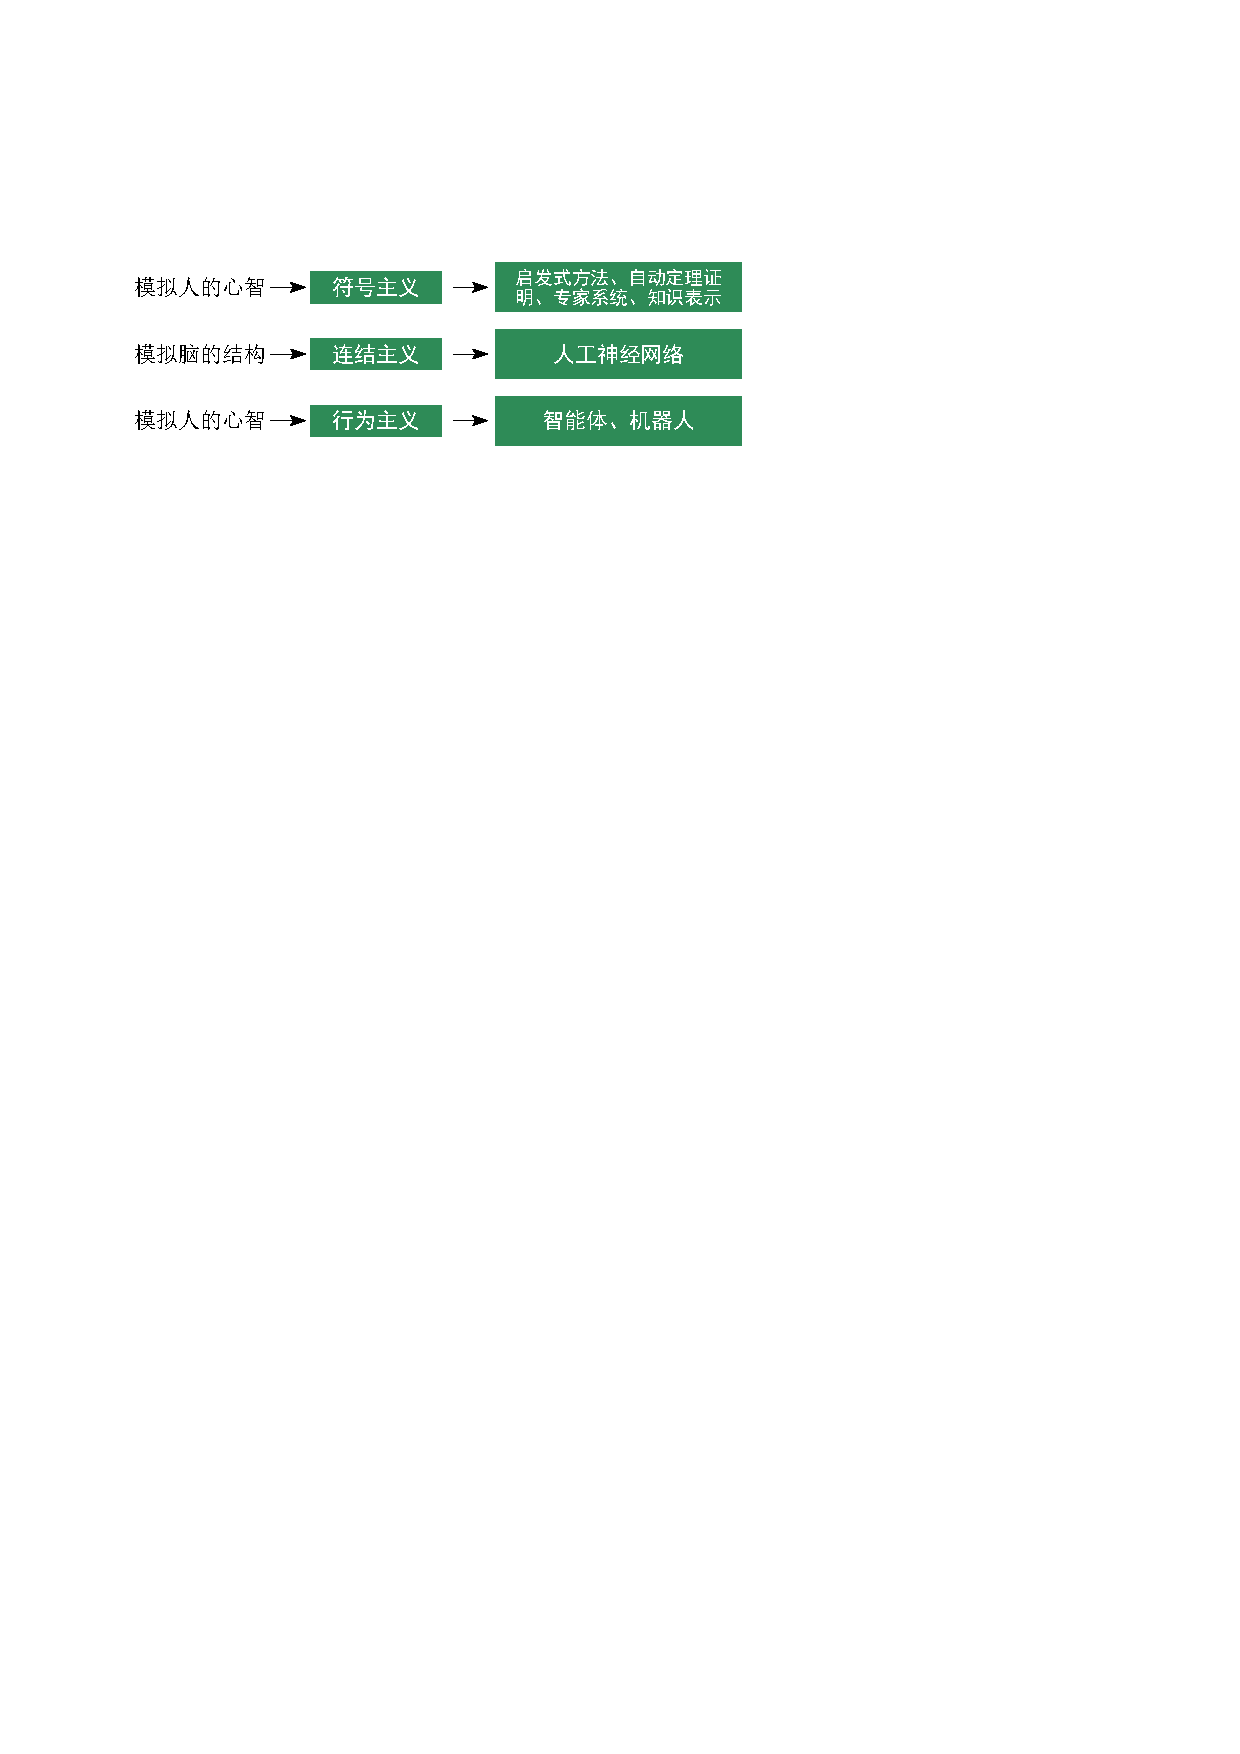
\includegraphics{image/3大学派.pdf}
\end{figure}
\begin{itemize}
    \item 符号主义学派的核心是符号演算与机器推理
    \item 连接主义学派的核心是神经网络与深度学习
    \item 行为主义学派推崇控制、自适应与进化计算
\end{itemize}

\subsection{Agent}
Agent是能够通过传感器感知环境,并且通过执行器对环境产生影响的任何东西。
\begin{figure}[htbp]
    \centering
    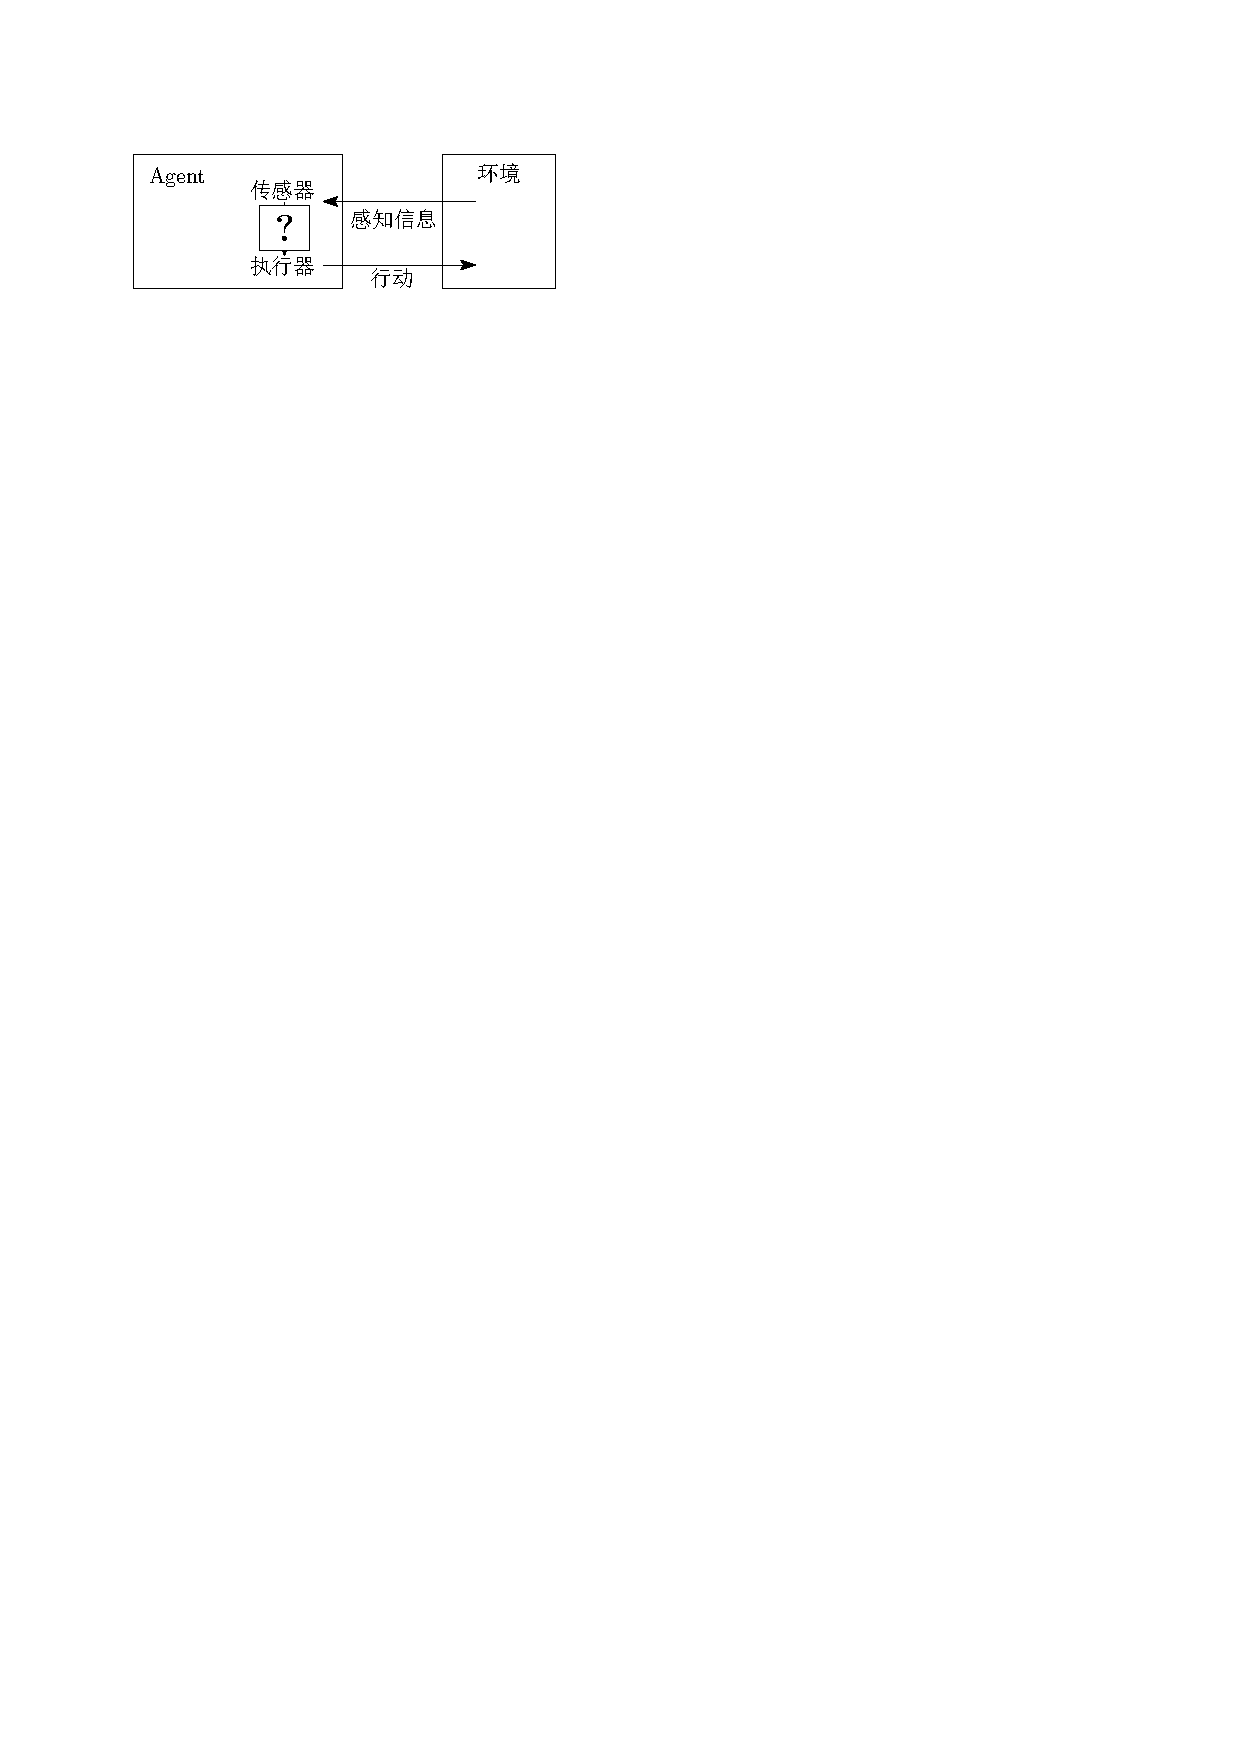
\includegraphics{image/Agent.pdf}
\end{figure}

\begin{itemize}
    \item Agent函数:将感知序列映射为行动:
    \[
        f:P^*\to A
    \]
    \item Agent程序:实现Agent函数,并在物理平台上运行
    \begin{center}
        \colorbox{main1}{Agent = 物理平台+\ Agent程序}
    \end{center}
\end{itemize}

Agent三个要素:
\begin{itemize}
    \item 感知环境能力
    \item 作用环境能力
    \item 感知信息与动作决策之间的映射机制
\end{itemize}

感知序列:
\begin{itemize}
    \item 有记忆
    \item 自身状态
    \item 之前的行为对当前决策与动作有影响
\end{itemize}

\begin{definition}[理性Agent]
    对每一个可能的感知信息,根据已知的感知序列提供的证据和Agent具有的先验知识,理性Agent应该选择能使其性能测度最大化的行动。
\end{definition}
\begin{definition}[性能测度]
    性能测度是对行动序列导致期望的环境变化的度量。
\end{definition}
性能测度对Agent的行为模型具有重要影响。

\begin{figure}[htbp]
    \centering
    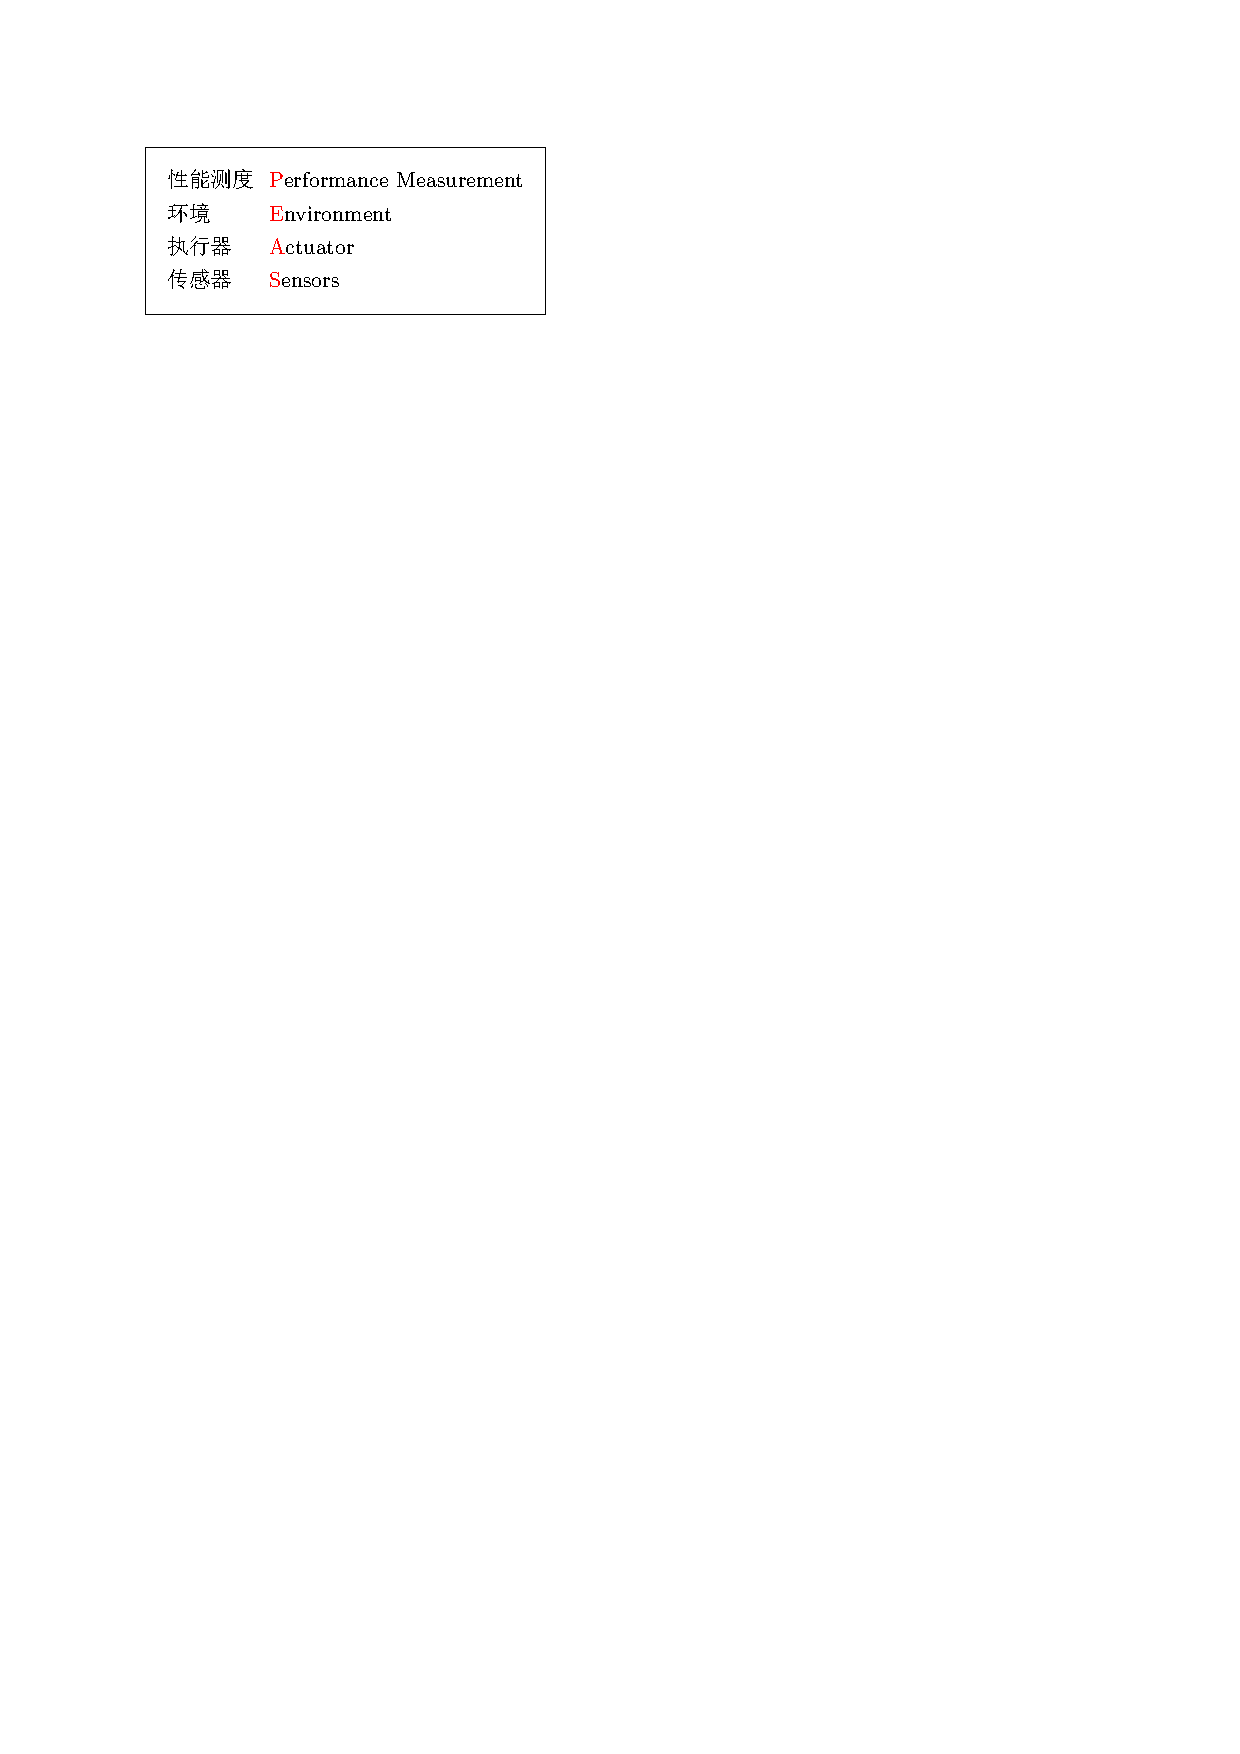
\includegraphics{image/PEAS.pdf}
\end{figure}

环境属性
\begin{itemize}
    \item 完全可观 vs 部分可观 (Fully observable vs. partially observable)
    \item 确定的 vs 随机的 (Deterministic vs. stochastic )
    \item 片段式vs 延续式(Episodic vs. sequential)
    \item 静态 vs 动态 (Dynamic vs. static )
    \item 离散 vs 连续 ( Discrete vs. continuous )
    \item 单Agent vs 多Agent ( Single agent vs. multi-agent )
    \item 已知 vs 未知 (Known vs. unknown)
\end{itemize}
% Table generated by Excel2LaTeX from sheet '环境属性'
\begin{table}[htbp]
    \centering
    \begin{tabular}{|c|ccc|}
      \hline
      任务环境 & 魔方Agnet & 吸尘器Agent & 无人侦察机 \bigstrut\\
      \hline
      完全可观 & 完全可观 & 部分可观 & 部分可观 \bigstrut[t]\\
      确定的 & 确定的 & 随机的 & 随机的 \\
      片段式 & 延续式 & 延续式 & 延续式 \\
      静态  & 静态  & 动态  & 动态 \\
      离散  & 离散  & 连续  & 连续 \\
      单Agent & 单   & 单   & 多 \\
      已知  & 已知  & 未知  & 未知 \bigstrut[b]\\
      \hline
    \end{tabular}%
\end{table}%

\begin{center}
    \colorbox{main1}{真实的环境是: 部分可观察、随机、延续、动态、连续、多Agent和未知。}
\end{center}
  
Agent类型:
\begin{figure}[htbp]
    \centering
    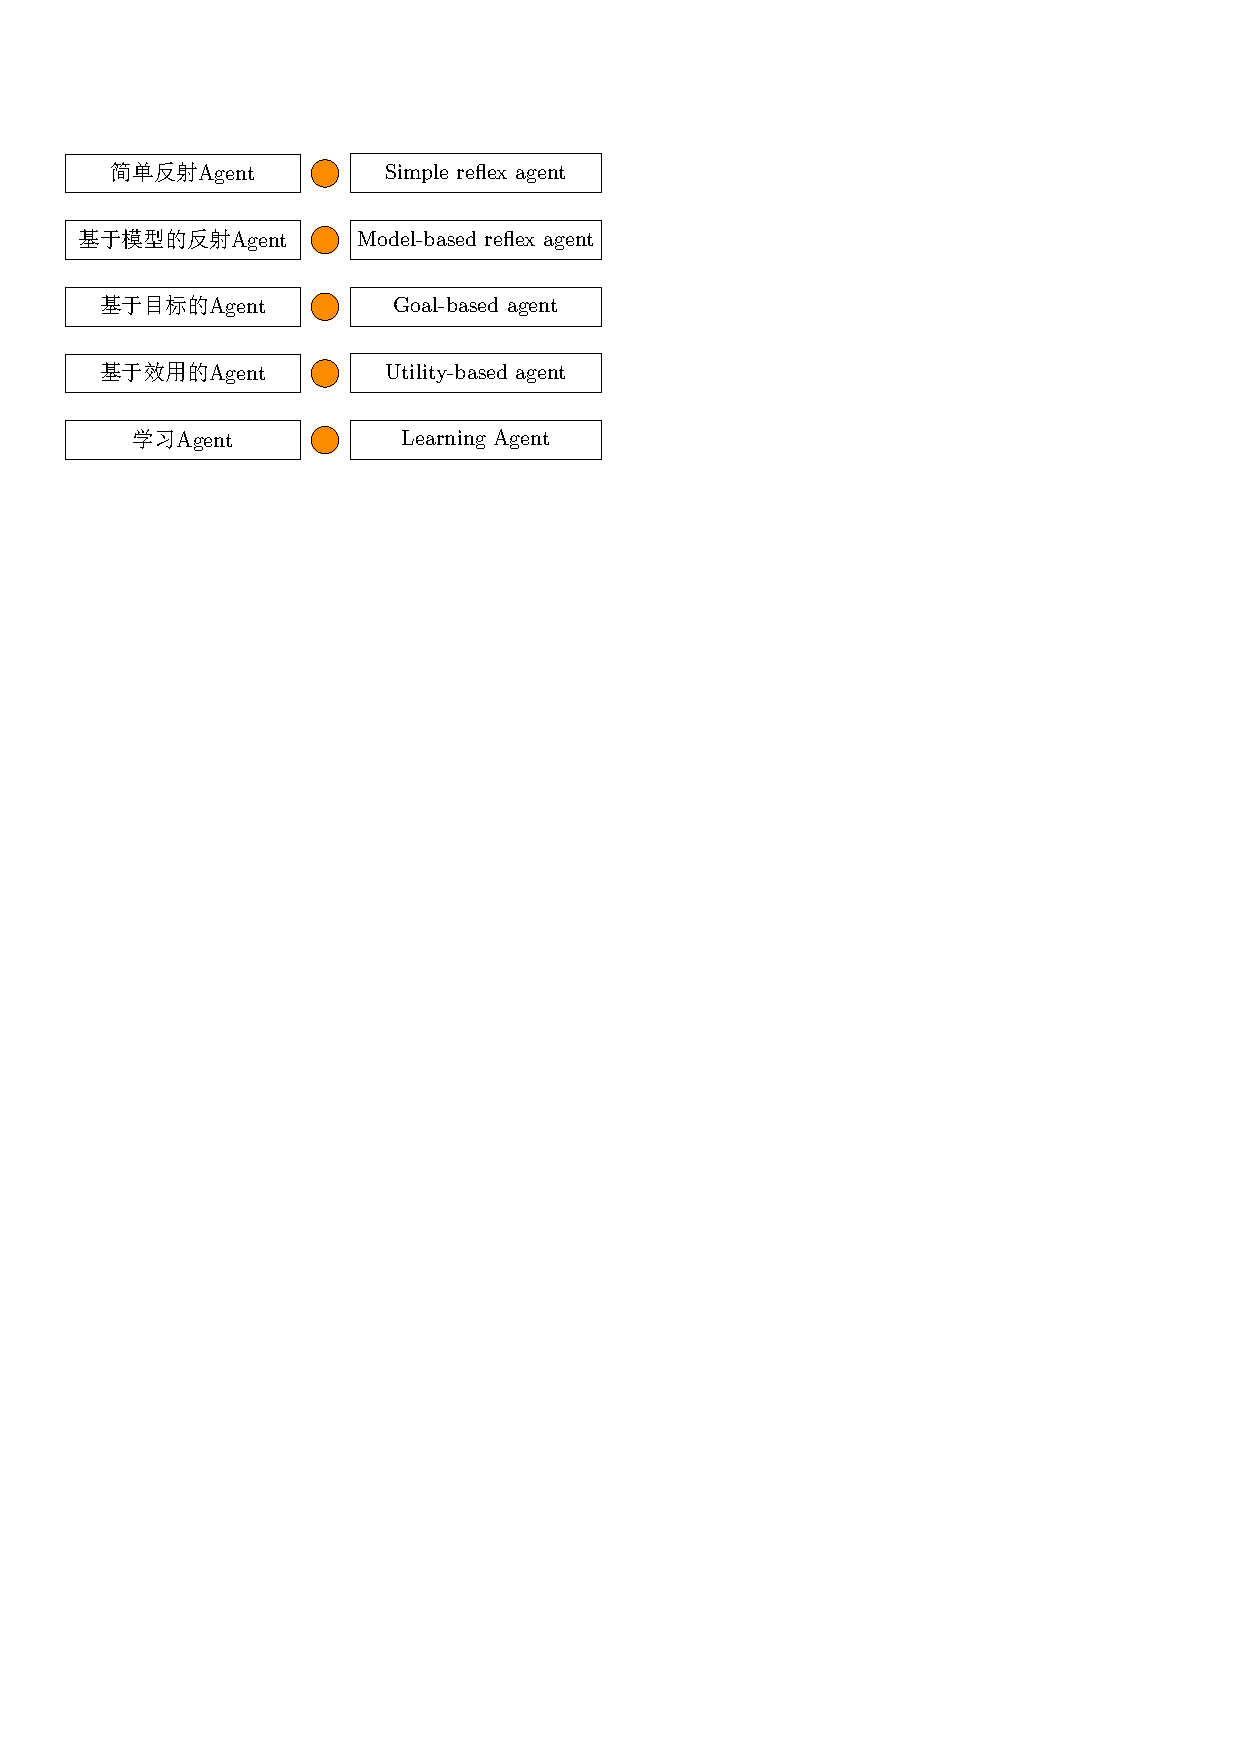
\includegraphics{image/Agent类型.pdf}
\end{figure}

\begin{definition}[简单反射Agent]
    简单反射Agent仅仅在当前感知的基础上动作忽略其余的感知历史。
\end{definition}
\begin{figure}[htbp]
    \centering
    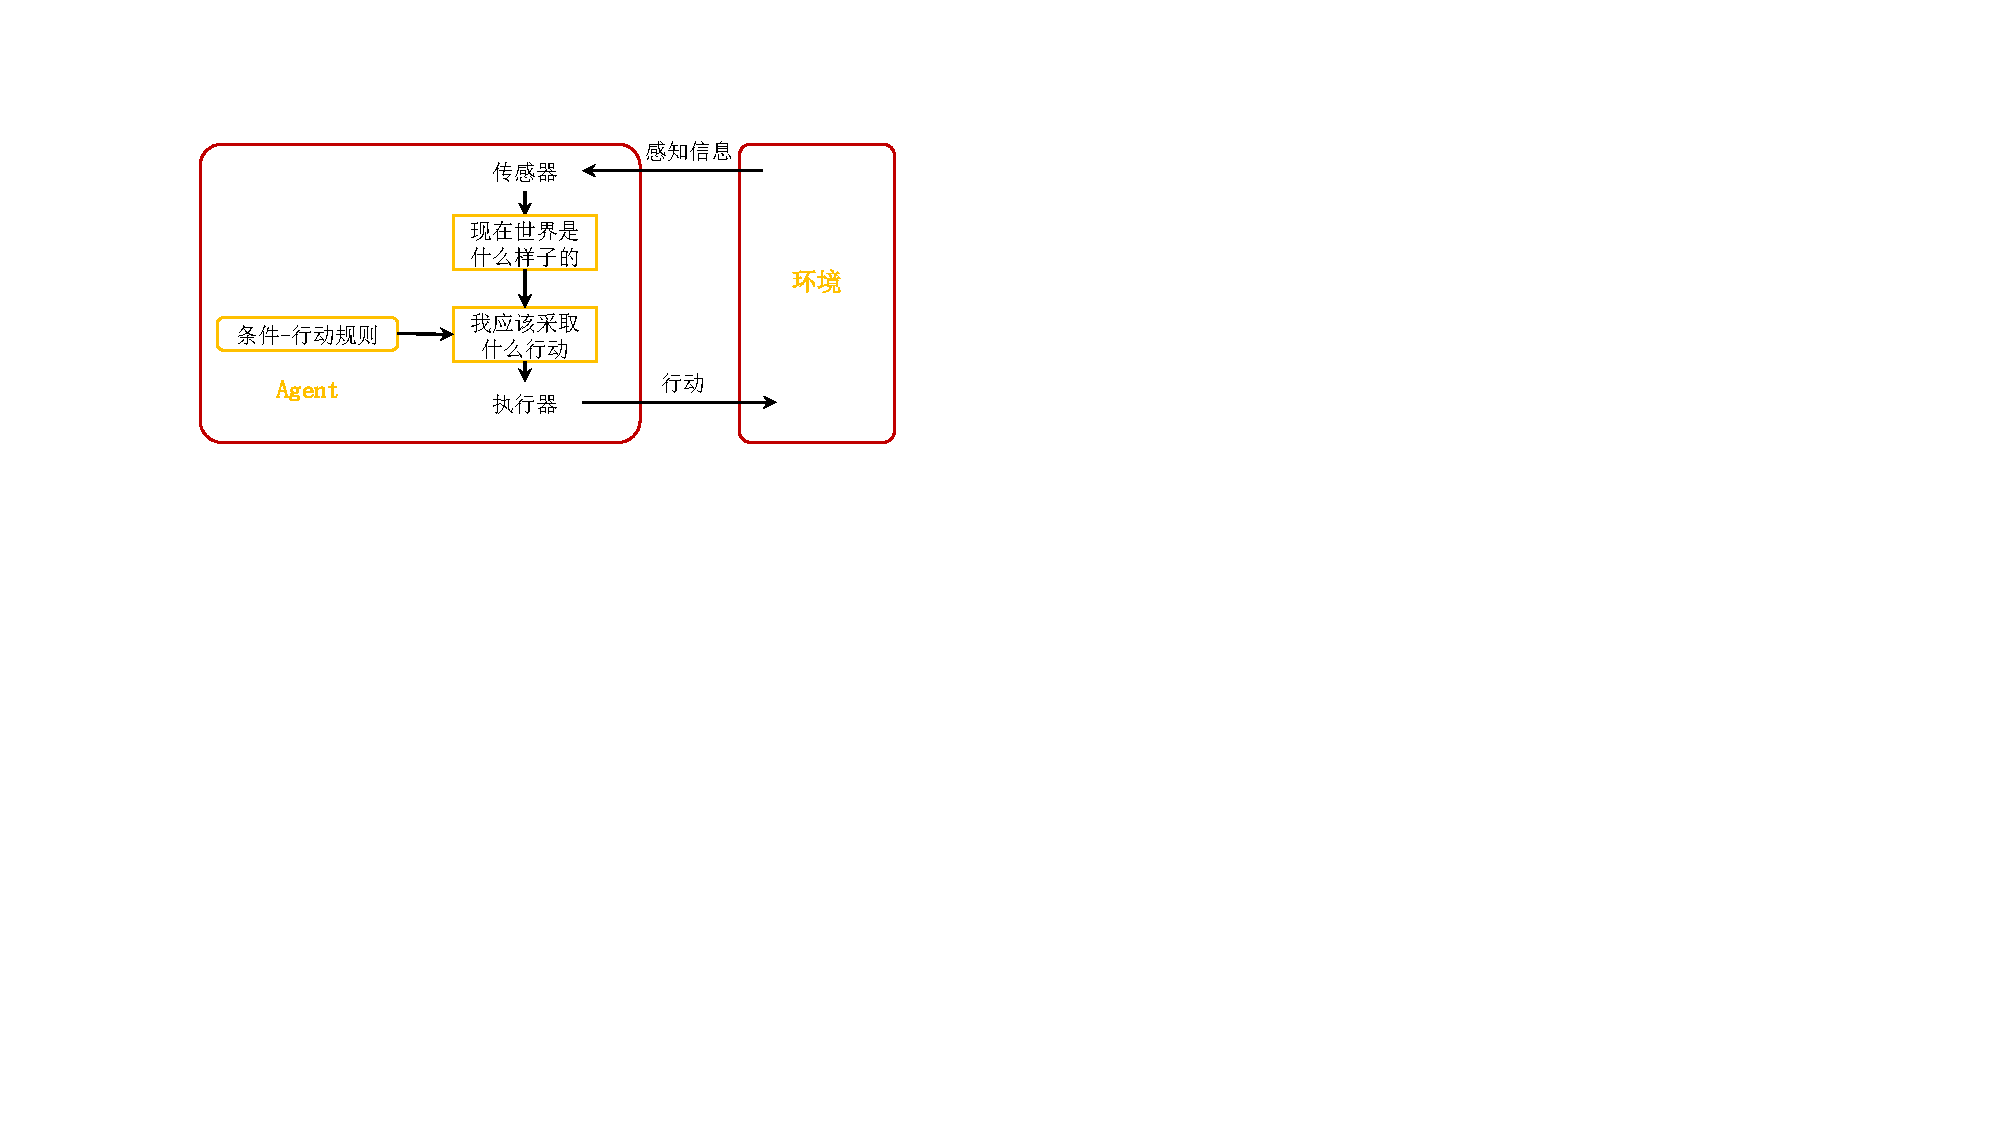
\includegraphics{image/简单反射Agent.pdf}
\end{figure}

\begin{definition}[基于模型的反射Agent]
    基于模型的反射Agent可以处理部分可观的环境。其当前状态存储在Agent内部,它描述不可见的环境的一部分。
\end{definition}
\begin{figure}[htbp]
    \centering
    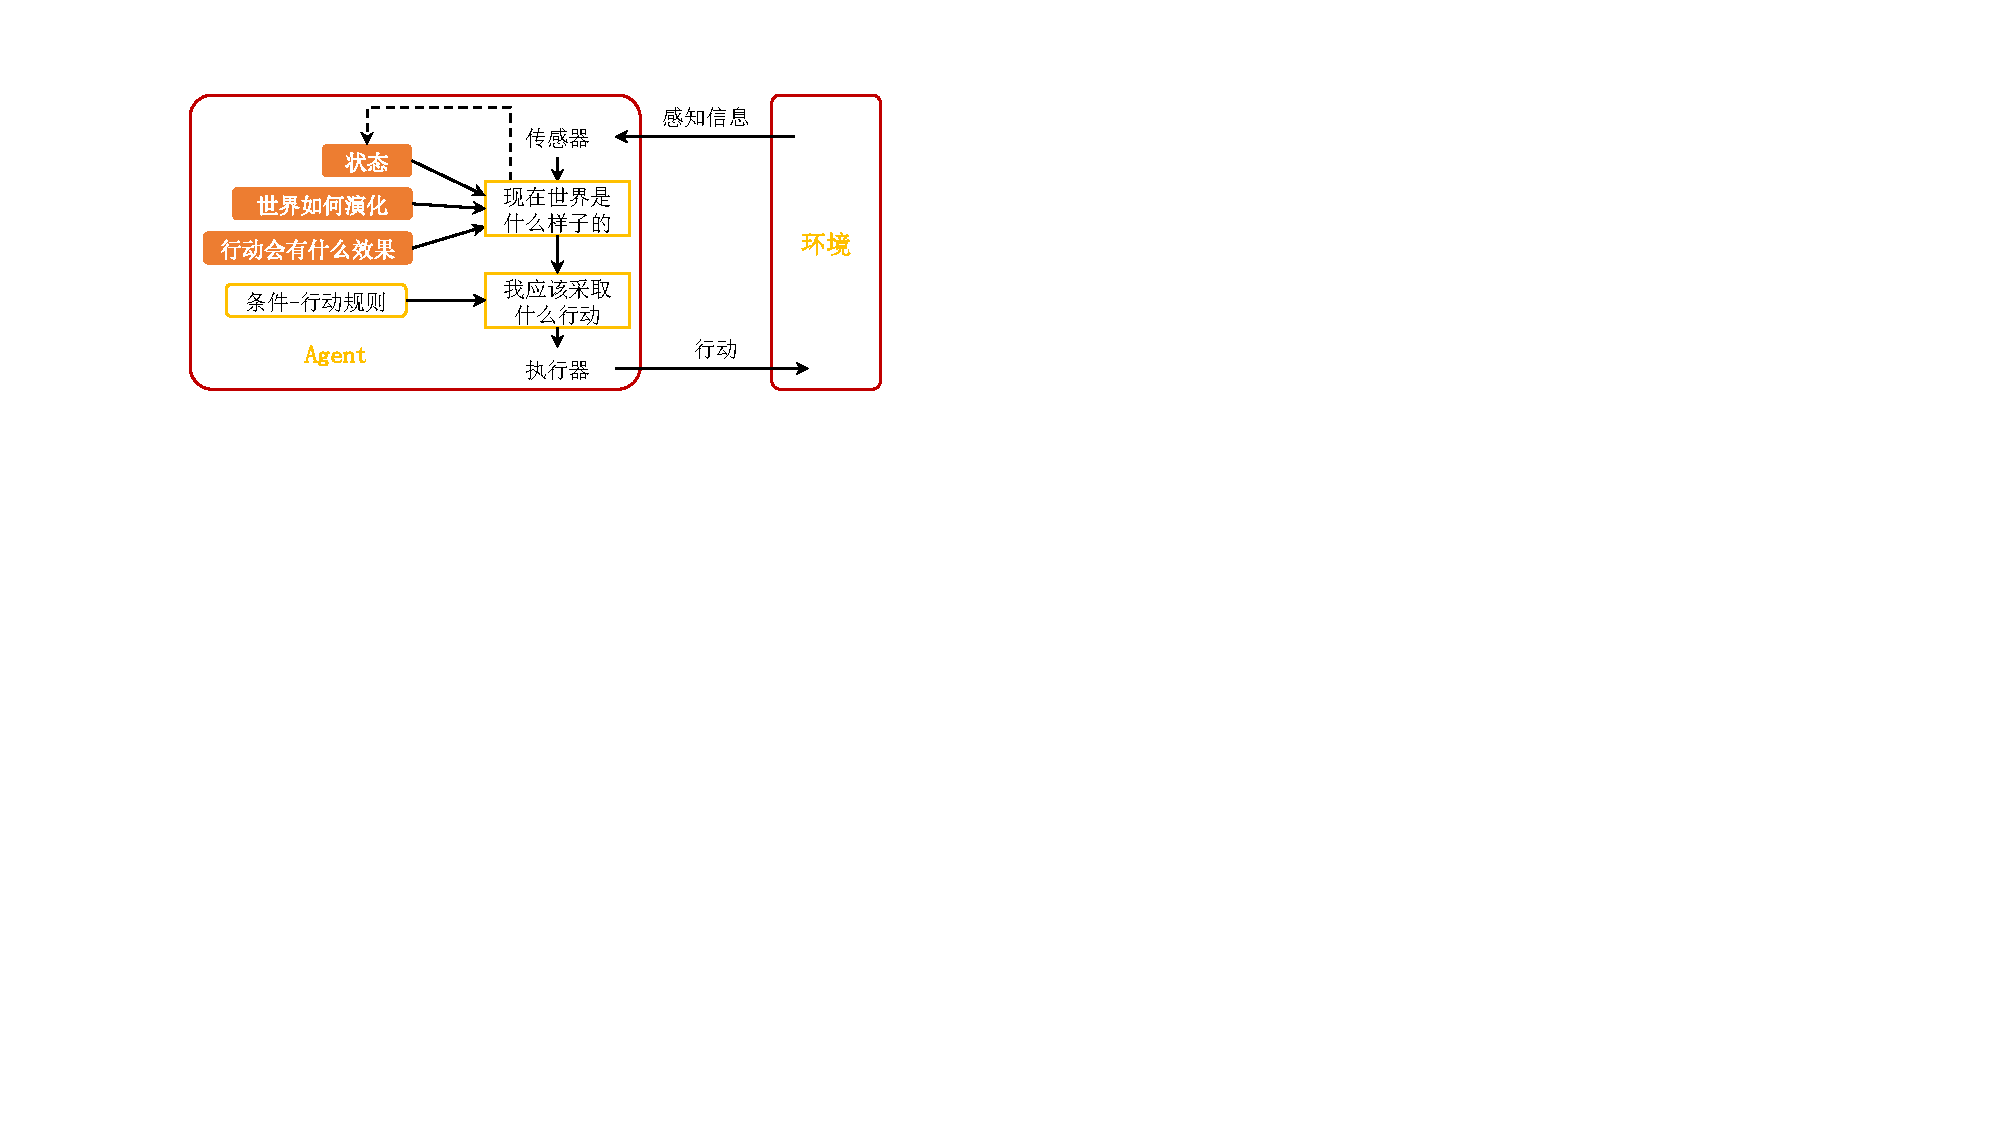
\includegraphics{image/基于模型的反射Agent.pdf}
\end{figure}

\begin{definition}[基于目标的Agent]
    利用“目标”信息,基于目标的Agent进一步扩展了基于模型的反射Agent的功能。  
\end{definition}
\begin{figure}[H]
    \centering
    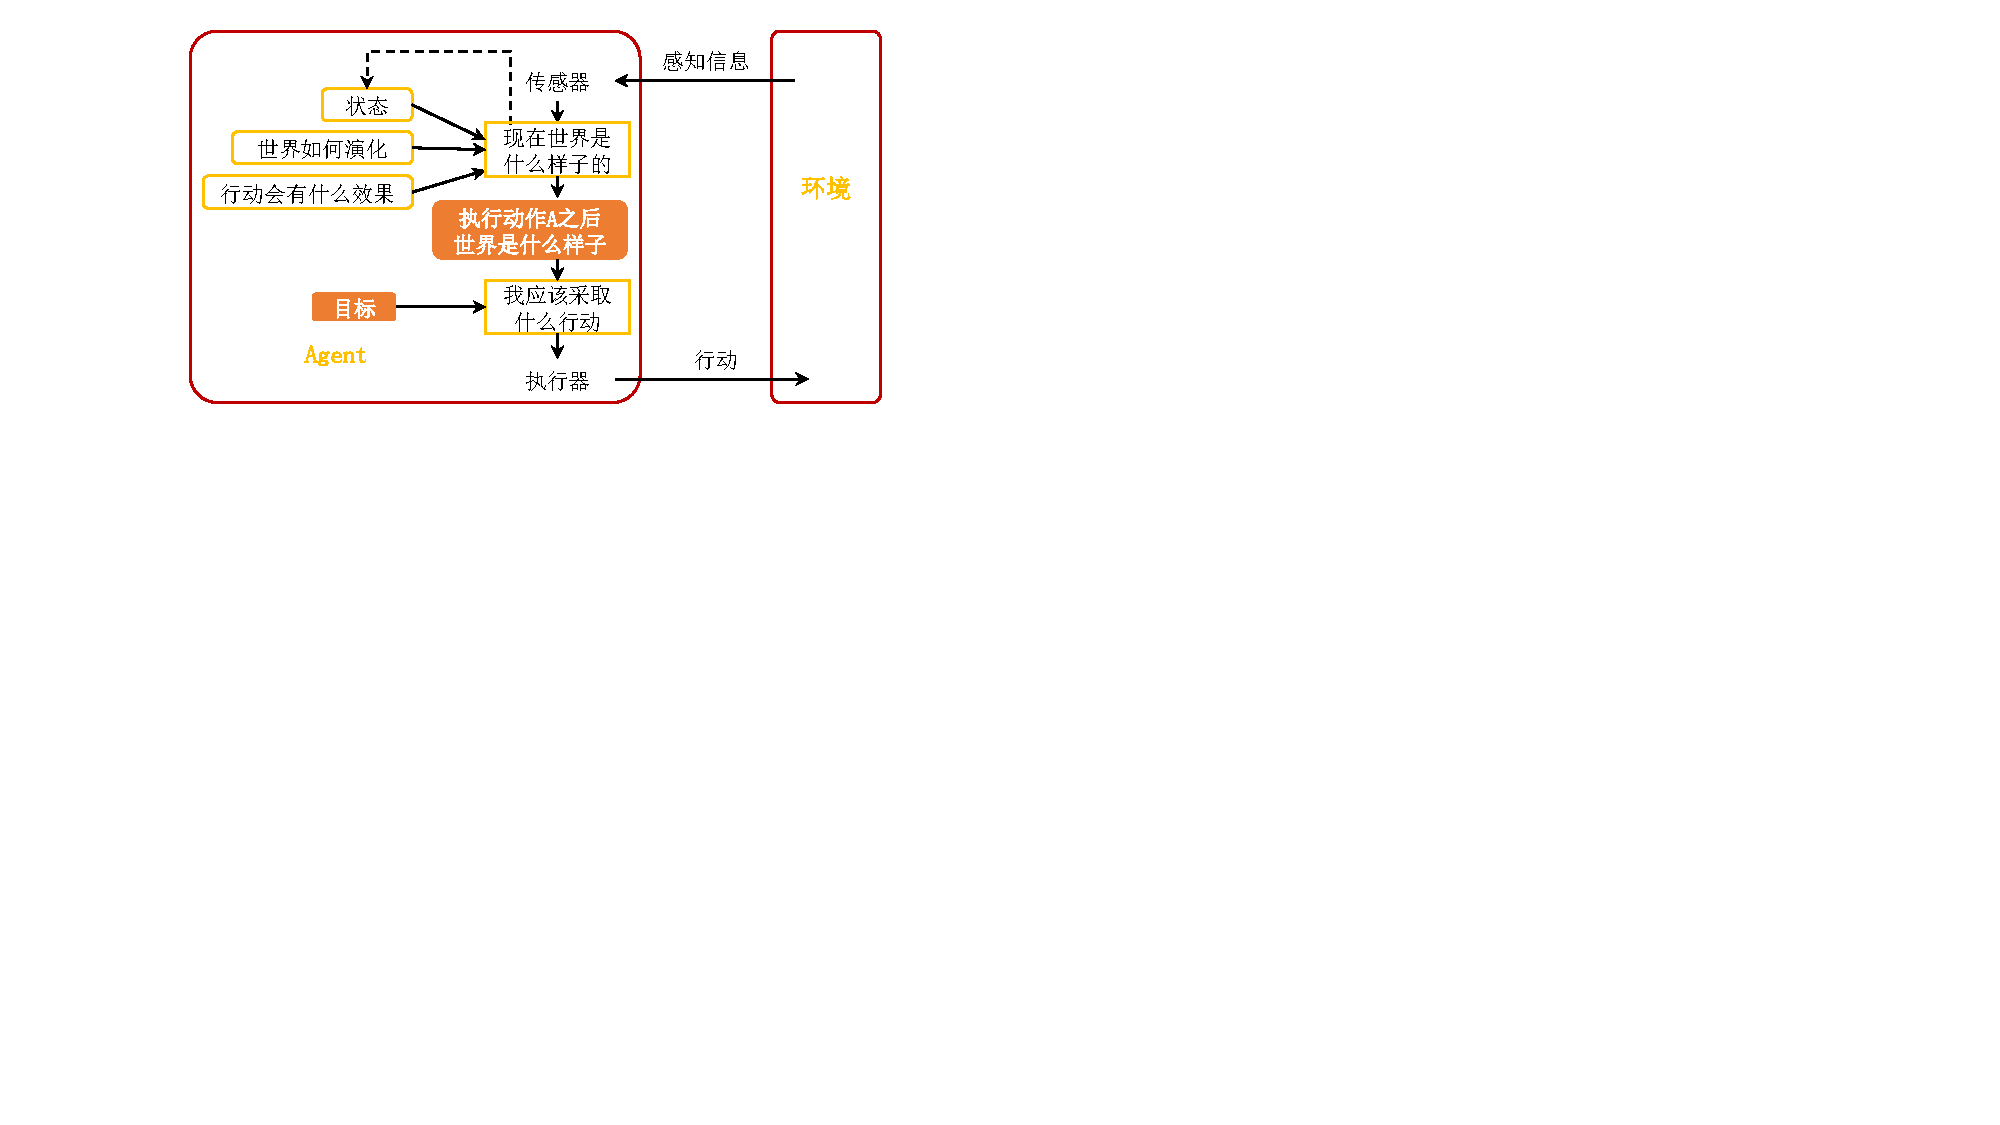
\includegraphics{image/基于目标的反射Agent.pdf}
\end{figure}

\begin{definition}[基于效用的Agent]
    使用效用函数得到对Agent的行动进行性能度量Agent选择最大效用的行动。
\end{definition}
\begin{figure}[H]
    \centering
    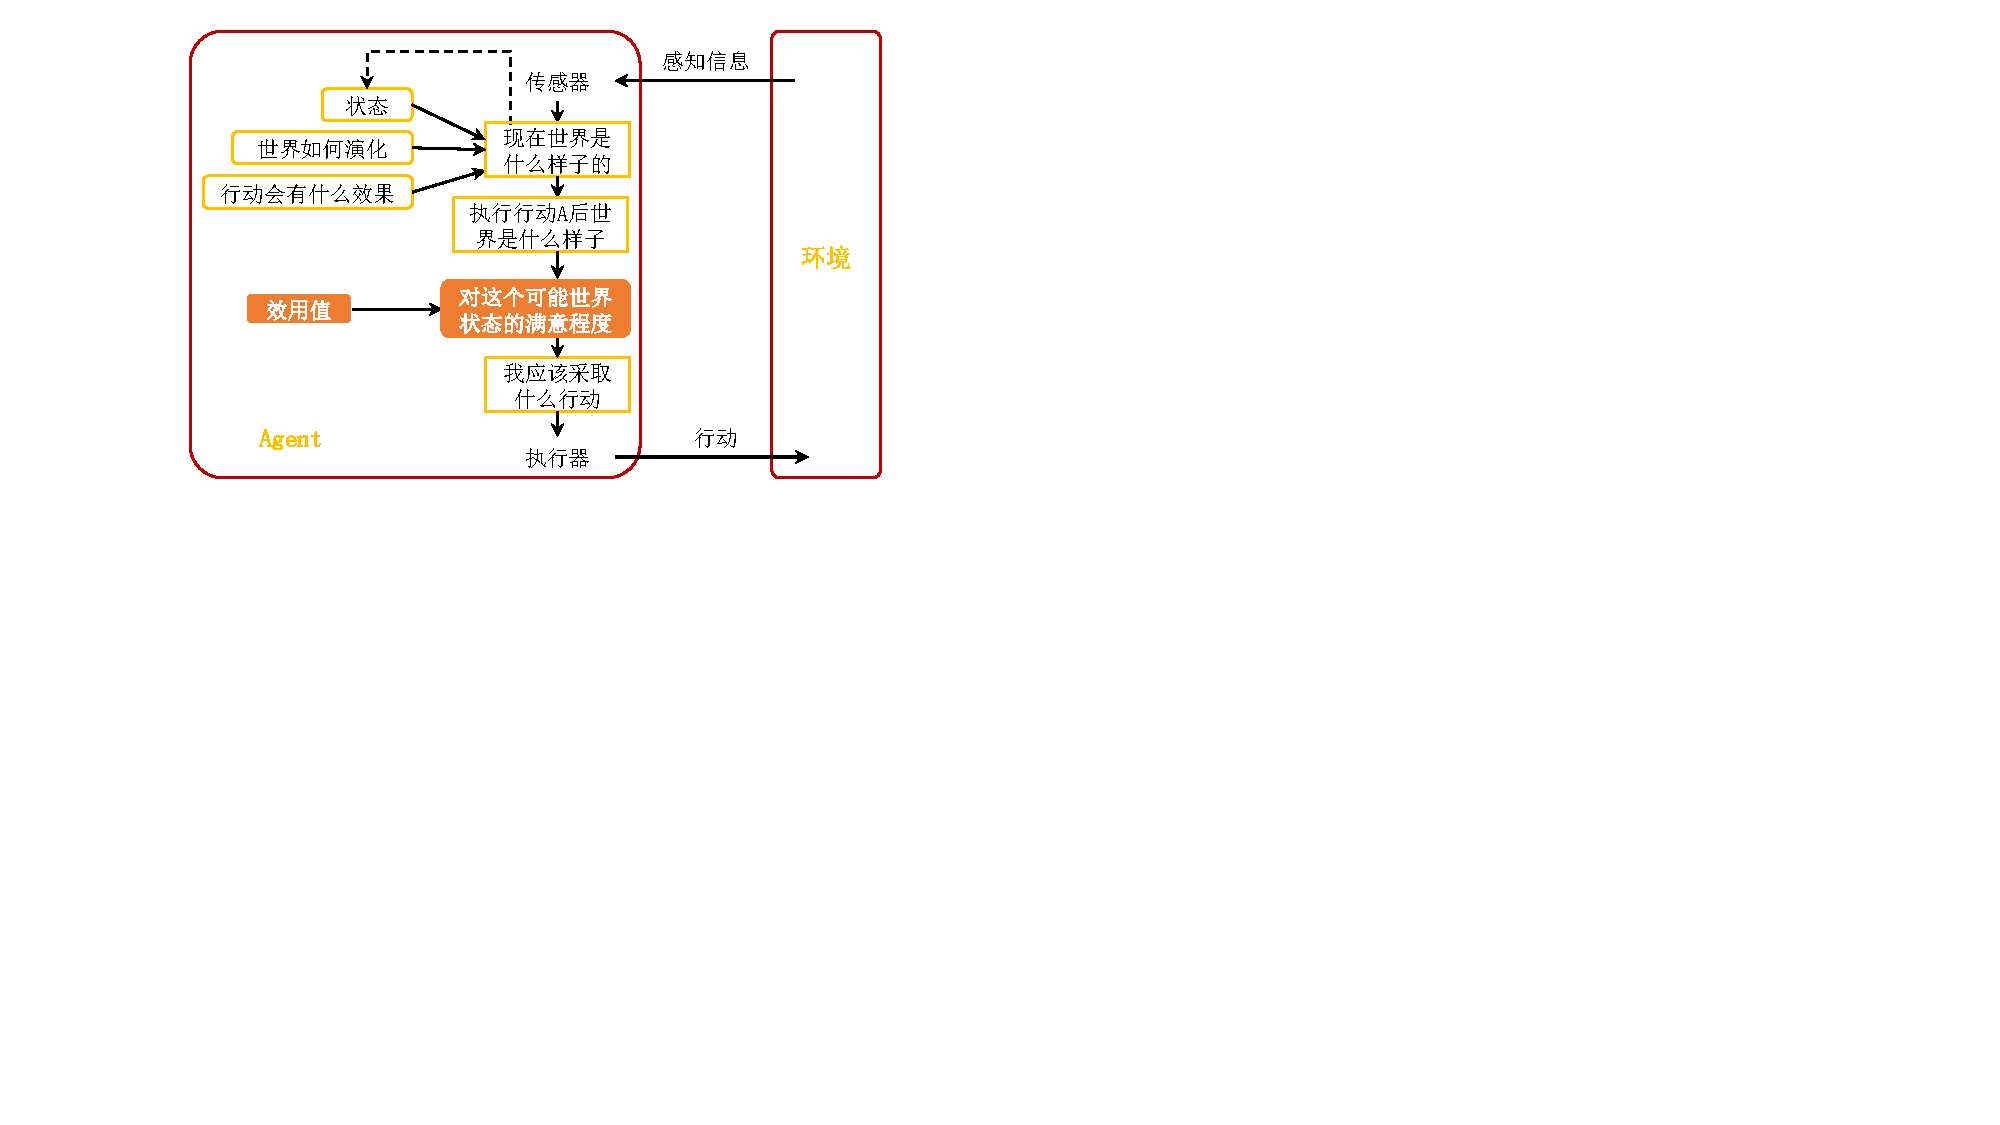
\includegraphics{image/基于效用的Agent.pdf}
\end{figure}

\begin{definition}[学习Agent]
    学习允许Agent在最初未知的环境中运行。与只具有最初知识相比,越来越胜任要执行的任务。 
\end{definition}
\begin{figure}[htbp]
    \centering
    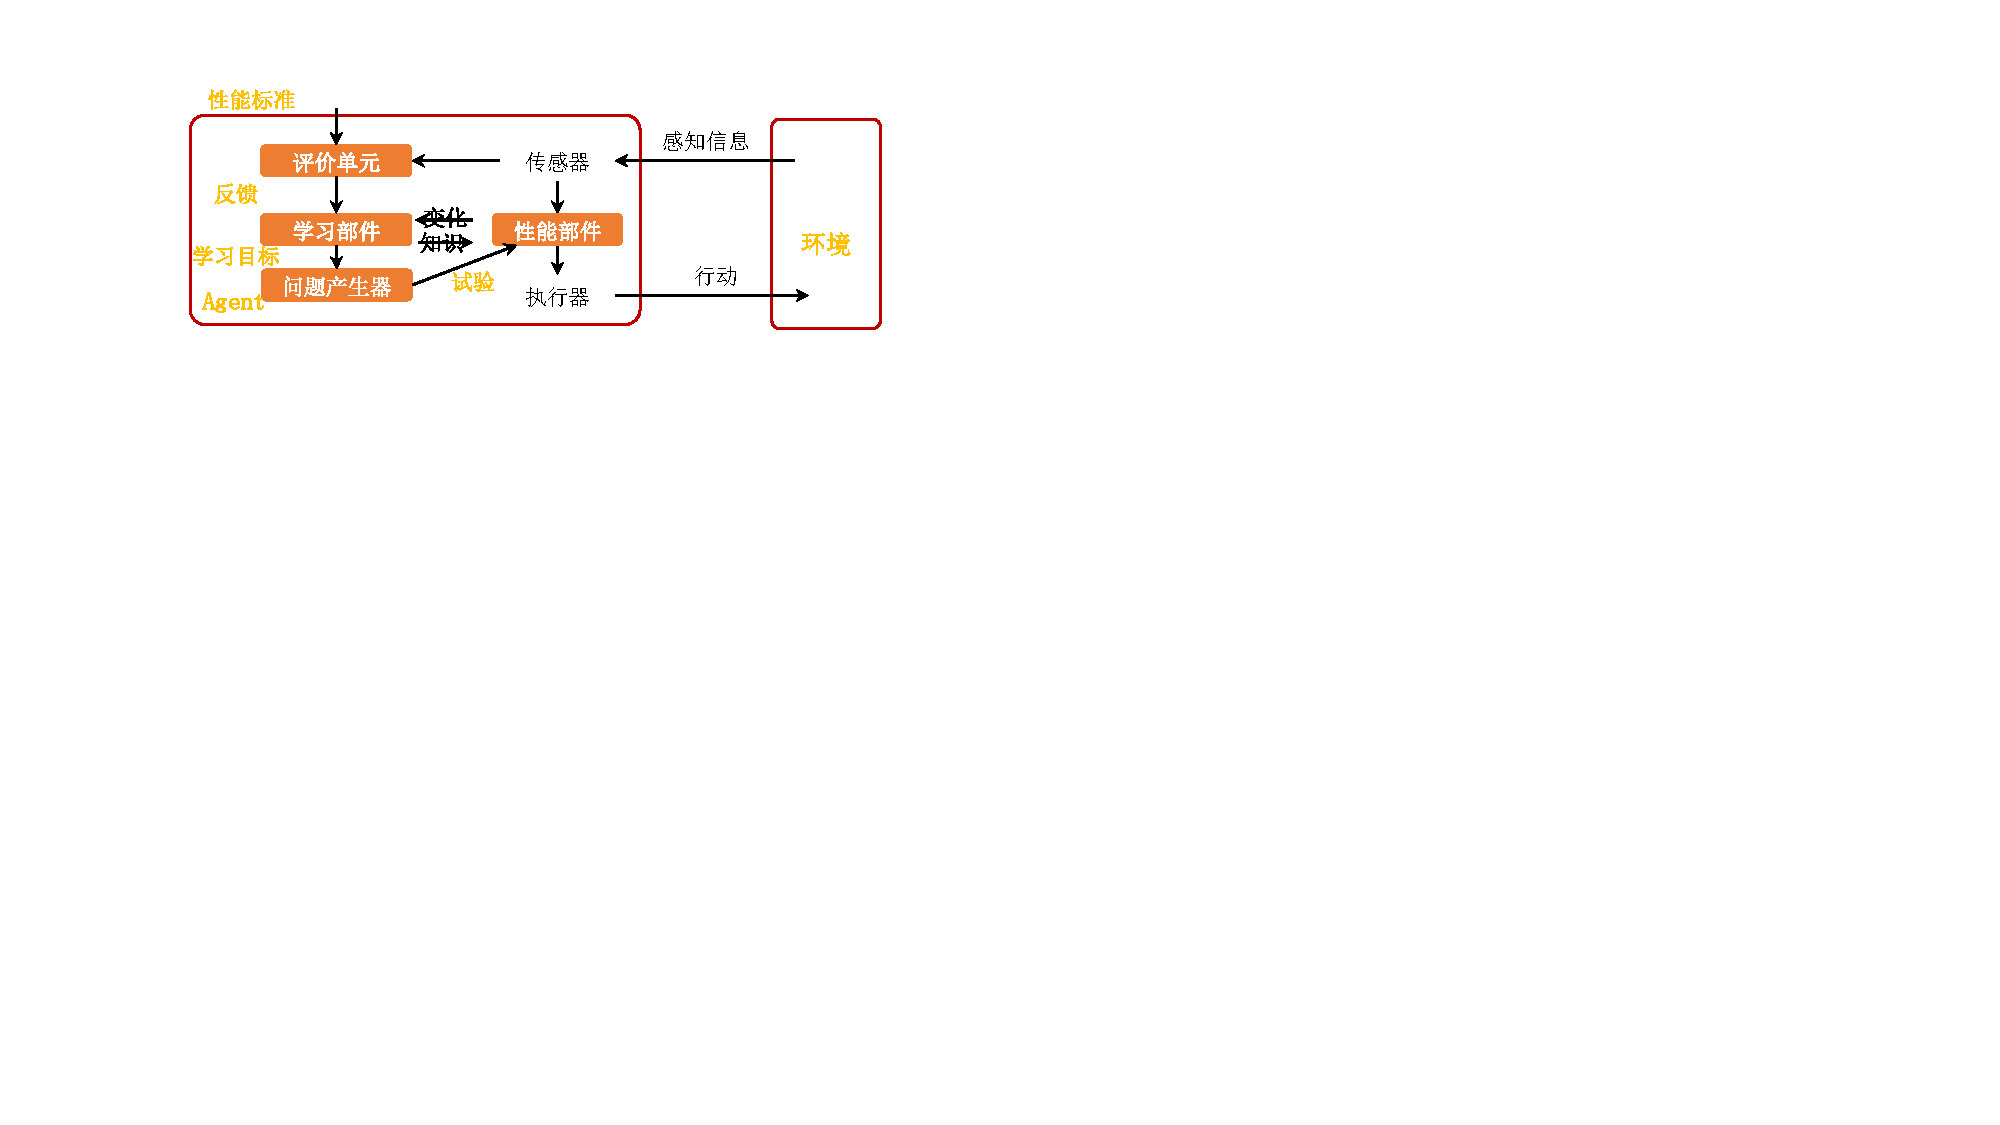
\includegraphics{image/学习Agent.pdf}
\end{figure}

表征环境状态的方式
\begin{itemize}
    \item 原子化
    
    每种状态都是内部结构未知的黑盒
    \item 要素化
    
    每种状态由固定的属性和值组成
    \item 结构化
    
    每个状态都包括对象,每个状态都具有与其他对象的属性和关系
\end{itemize}

  
  
\section{搜索}
\subsection{基本搜索算法}
\subsubsection{树搜索算法和图搜索算法}
\begin{figure}[htbp]
    \centering
    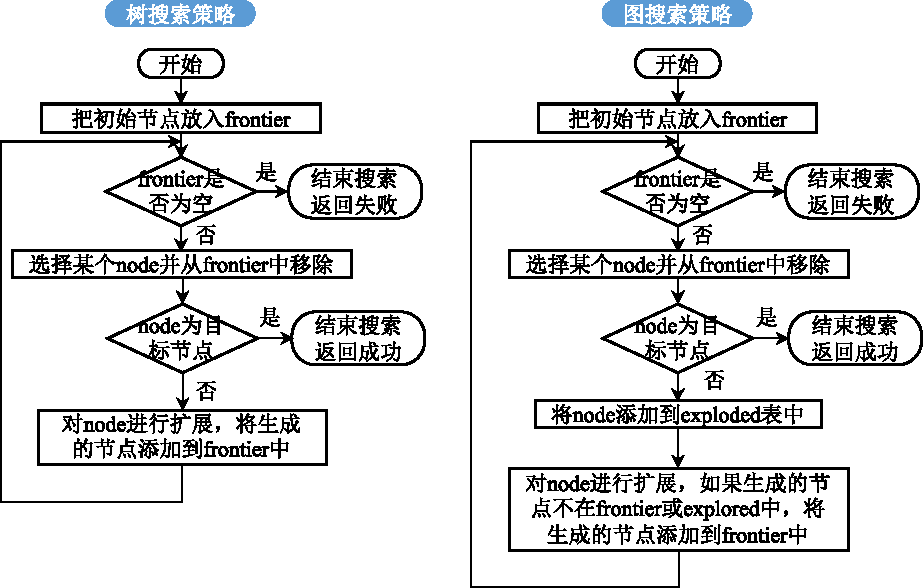
\includegraphics{image/图搜索和树搜索.pdf}
\end{figure}
\subsection{盲目搜素策略}
\begin{example}
    如图,$S$为初始状态,$G_1$和$G_2$为目标状态。忽略各状态之间的代价,注意连线是有方向的。在其他条件都相同的情况下,按照字母先后顺序对节点进行扩展。
    \begin{figure}[htbp]
        \centering
        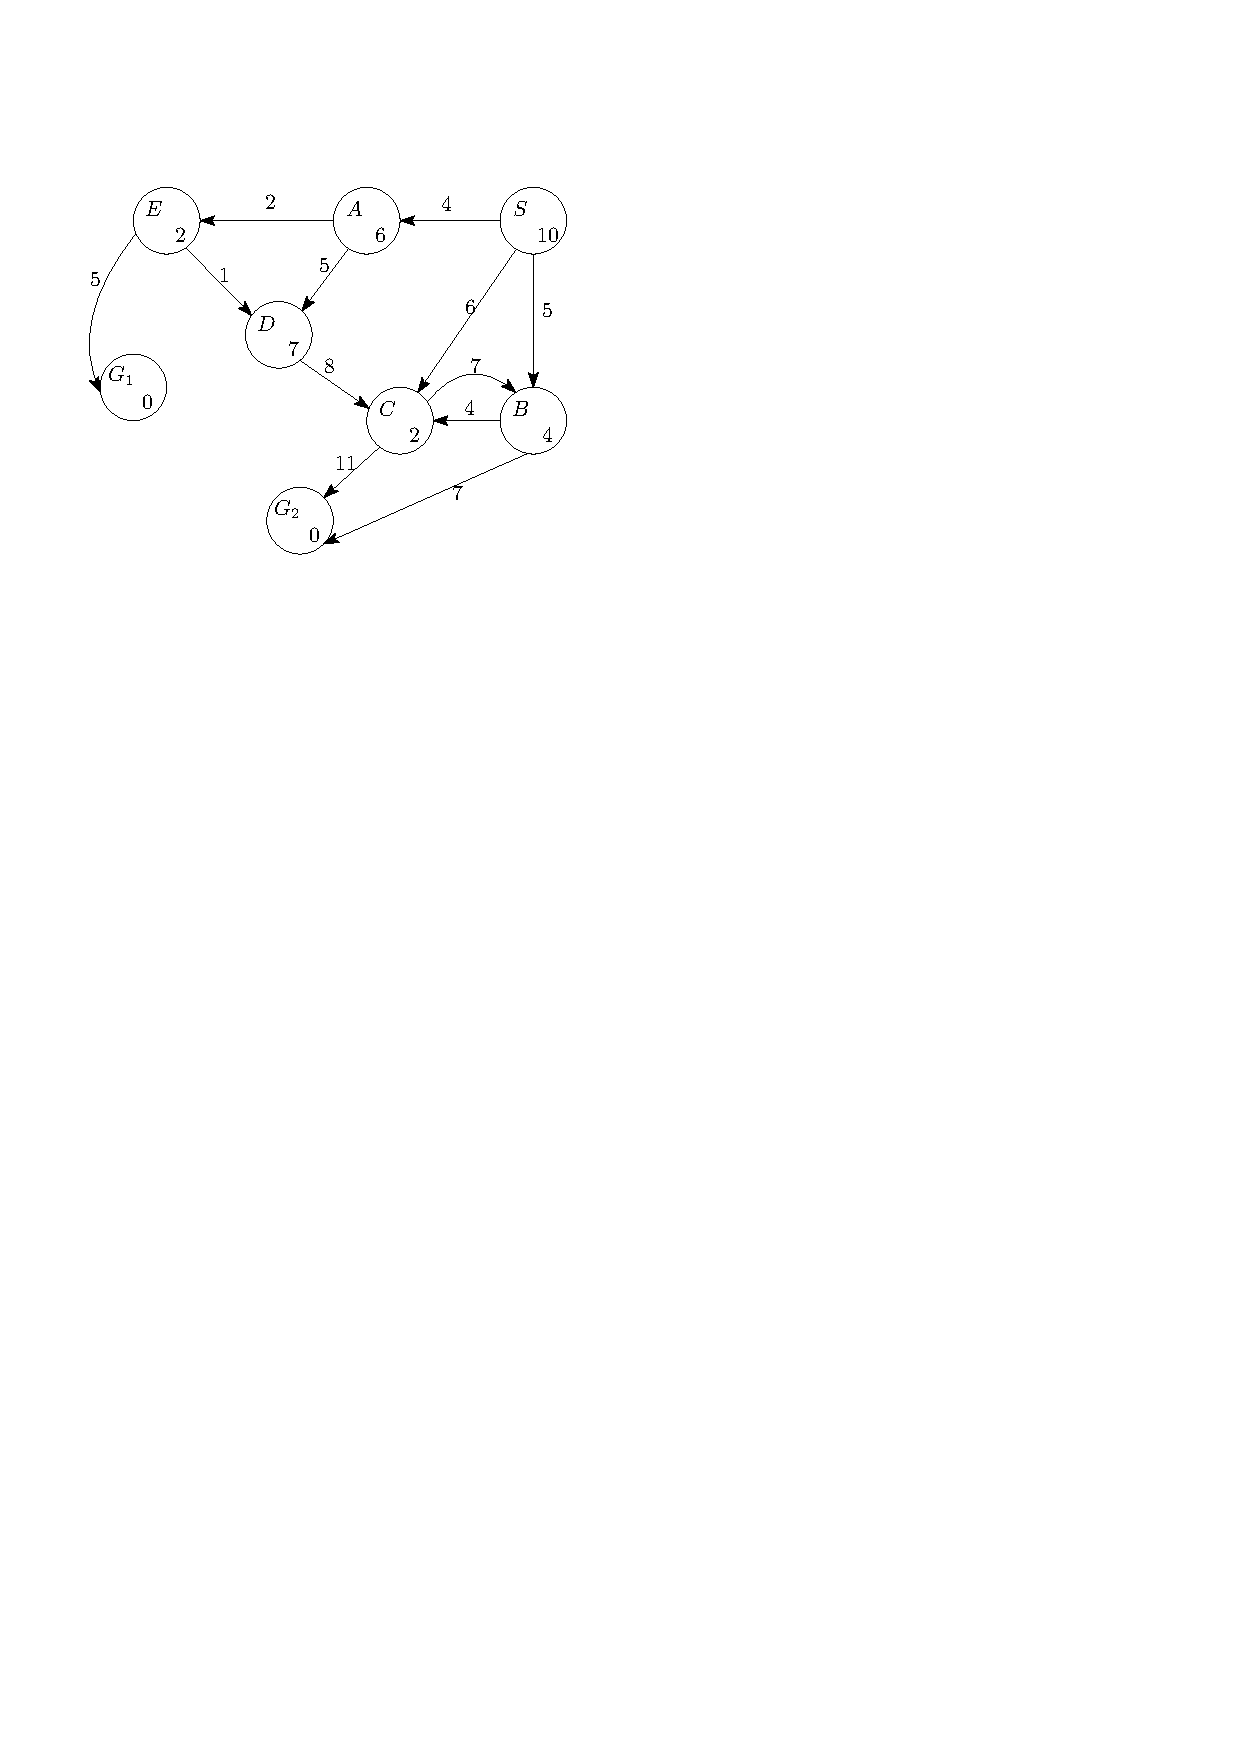
\includegraphics{image/搜索策略例题.pdf}
    \end{figure}
    \begin{enumerate}
        \item 应用\textcolor{main1}{宽度优先搜索}策略,指出\textcolor{main1}{树搜索}算法将会到达的目标状态,并按顺序写出搜索过程中所扩展出的节点。
        \item 应用\textcolor{main1}{宽度优先搜索}策略,指出\textcolor{main1}{图搜索}算法将会到达的目标状态,并按顺序写出搜索过程中所扩展出的节点。
    \end{enumerate}
    
    \textcolor{main1}{树搜索}:达到目标状态为$G_2$,解序列:$S\to B\to G_2$
    % Table generated by Excel2LaTeX from sheet '树搜索'
    \begin{table}[htbp]
        \centering
        \begin{tabular}{cc}
            \toprule[1.5pt]
            Step & frontier \\
            \midrule[1pt]
            Step 1 & $A,\, B,\, C$ \\
            Step 2 & $B,\, C,\, D,\, E$ \\
            Step 3 & $C,\, D,\, E,\, C,\, G_2$ \\
            Step 4 & $D,\, E,\, C,\, G_2,\, B,\, G_2$ \\
            Step 5 & $E,\, C,\, G_2,\, B,\, G_2,\, C$ \\
            Step 6 & $C,\, G_2,\, B,\, G_2,\, C,\, D,\, G_1$ \\
            Step 7 & $G_2,\, B,\, G_2,\, C,\, D,\, G_1,\, B,\, G_2$ \\
            \bottomrule[1.5pt]
        \end{tabular}%
    \end{table}%
  
    \textcolor{main1}{图搜索}:达到目标状态为$G_2$,解序列:$S\to B\to G_2$
    % Table generated by Excel2LaTeX from sheet '图搜索'
    \begin{table}[htbp]
        \centering
        \begin{tabular}{ccc}
        \toprule[1.5pt]
            Step & frontier & explored \\
            \midrule[1pt]
            Step 1 & $A,\, B,\, C$ & $S$ \\
            Step 2 & $B,\, C,\, D,\, E$ & $S,\, A$ \\
            Step 3 & $C,\, D,\, E,\, G_2$ & $S,\, A,\, B$ \\
            Step 4 & $D,\, E,\, G_2$ & $S,\, A,\, B,\, C$ \\
            Step 5 & $E,\, G_2$ & $S,\, A,\, B,\, C,\, D$ \\
            Step 6 & $G_2,\, G_1$ & $S,\, A,\, B,\, C,\, D,\, E$ \\
        \bottomrule[1.5pt]
        \end{tabular}%
    \end{table}%
\end{example}
\subsection{最佳优先搜索}
\subsubsection{评价函数}
\begin{definition}[评价函数]
    用来\textcolor{main1}{估算}经过节点$n$的路径代价的函数叫做\textcolor{main1}{评价函数},也称\textcolor{main1}{评估函数},用$f(n)$表示。
\end{definition}
\begin{note}
    路径的代价包括两部分:
    \begin{itemize}
        \item 一部分是确定性的代价。从起点到$n$的路径已经探索出来了,所耗费的代价可以精确计算,记为$g(n)$
        \item 一部分是不确定的代价。从$n$到终点的可能路径还没有探索出来,其代价只能进行预估,记为$h(n)$
    \end{itemize}
    \[
        f(n) = g(n) + h(n)
    \]
\end{note}
\subsubsection{一致代价搜索}
\begin{definition}[一致代价搜索]
    从初始状态到节点$n$已经产生的代价,\textcolor{main1}{无信息搜索策略}
    \[
        f(n) = g(n)
    \]
\end{definition}


\subsubsection{贪婪搜索}
\begin{definition}[贪婪搜索]
    贪婪搜索
    \[
        f(n) = h(n)
    \]
\end{definition}


\subsubsection{A\texorpdfstring{\textsuperscript{*}}{*}搜索}
\begin{definition}[A\textsuperscript{*}搜索]
    A\textsuperscript{*}搜索
    \[
        f(n) = g(n) + h(n)
    \]
\end{definition}

\begin{table}[htbp]
    \centering
    \resizebox{.95\textwidth}{!}{%
    \begin{tabular}{@{}cccc@{}}
    \toprule[1.5pt]
    搜索策略 & 一致代价 & 贪婪最佳优先 & A* \\ \midrule[1pt]
    评估函数 & $g(n)$ & $h(n)$ & $g(n)+h(n)$ \\
    完备性 & \begin{tabular}[c]{@{}c@{}}\textcolor{main1}{Yes*}:每步代价都>$\varepsilon>0$\\ 即无零代价步(图、树)\end{tabular} & \begin{tabular}[c]{@{}c@{}}\textcolor{main1}{树搜索}:否\\ 有限状态图搜索:是\end{tabular} & \multirow{2}{*}{\begin{tabular}[c]{@{}c@{}}$h(n)$若满足特定条件:\\ A*即完备且最优\end{tabular}} \\
    最优性 & \begin{tabular}[c]{@{}c@{}}\textcolor{main1}{Yes*}:比最优解代价小\\ 的节点数目优先(图、树)\end{tabular} & 否 &  \\
    时间复杂度 & $b^{1+[C^*/\varepsilon]}$ & \begin{tabular}[c]{@{}c@{}}$b^m$,\\ $m$搜索空间最大深度\end{tabular} & \multirow{2}{*}{\begin{tabular}[c]{@{}c@{}}扩展节点以解路径的长度呈指数增长。对于每\\ 步骤代价为常量的问题时间复杂度是最优解\\ 所在深度$d$的函数。\end{tabular}} \\
    空间复杂度 & $b^{1+[C^*/\varepsilon]}$ & \begin{tabular}[c]{@{}c@{}}$b^m$,\\ 保存所有节点在内存中\end{tabular} &  \\ \bottomrule[1.5pt]
    \end{tabular}%
    }
\end{table}
\begin{example}
    试用以下算法进行求解进行求解。
    \begin{figure}[H]
        \centering
        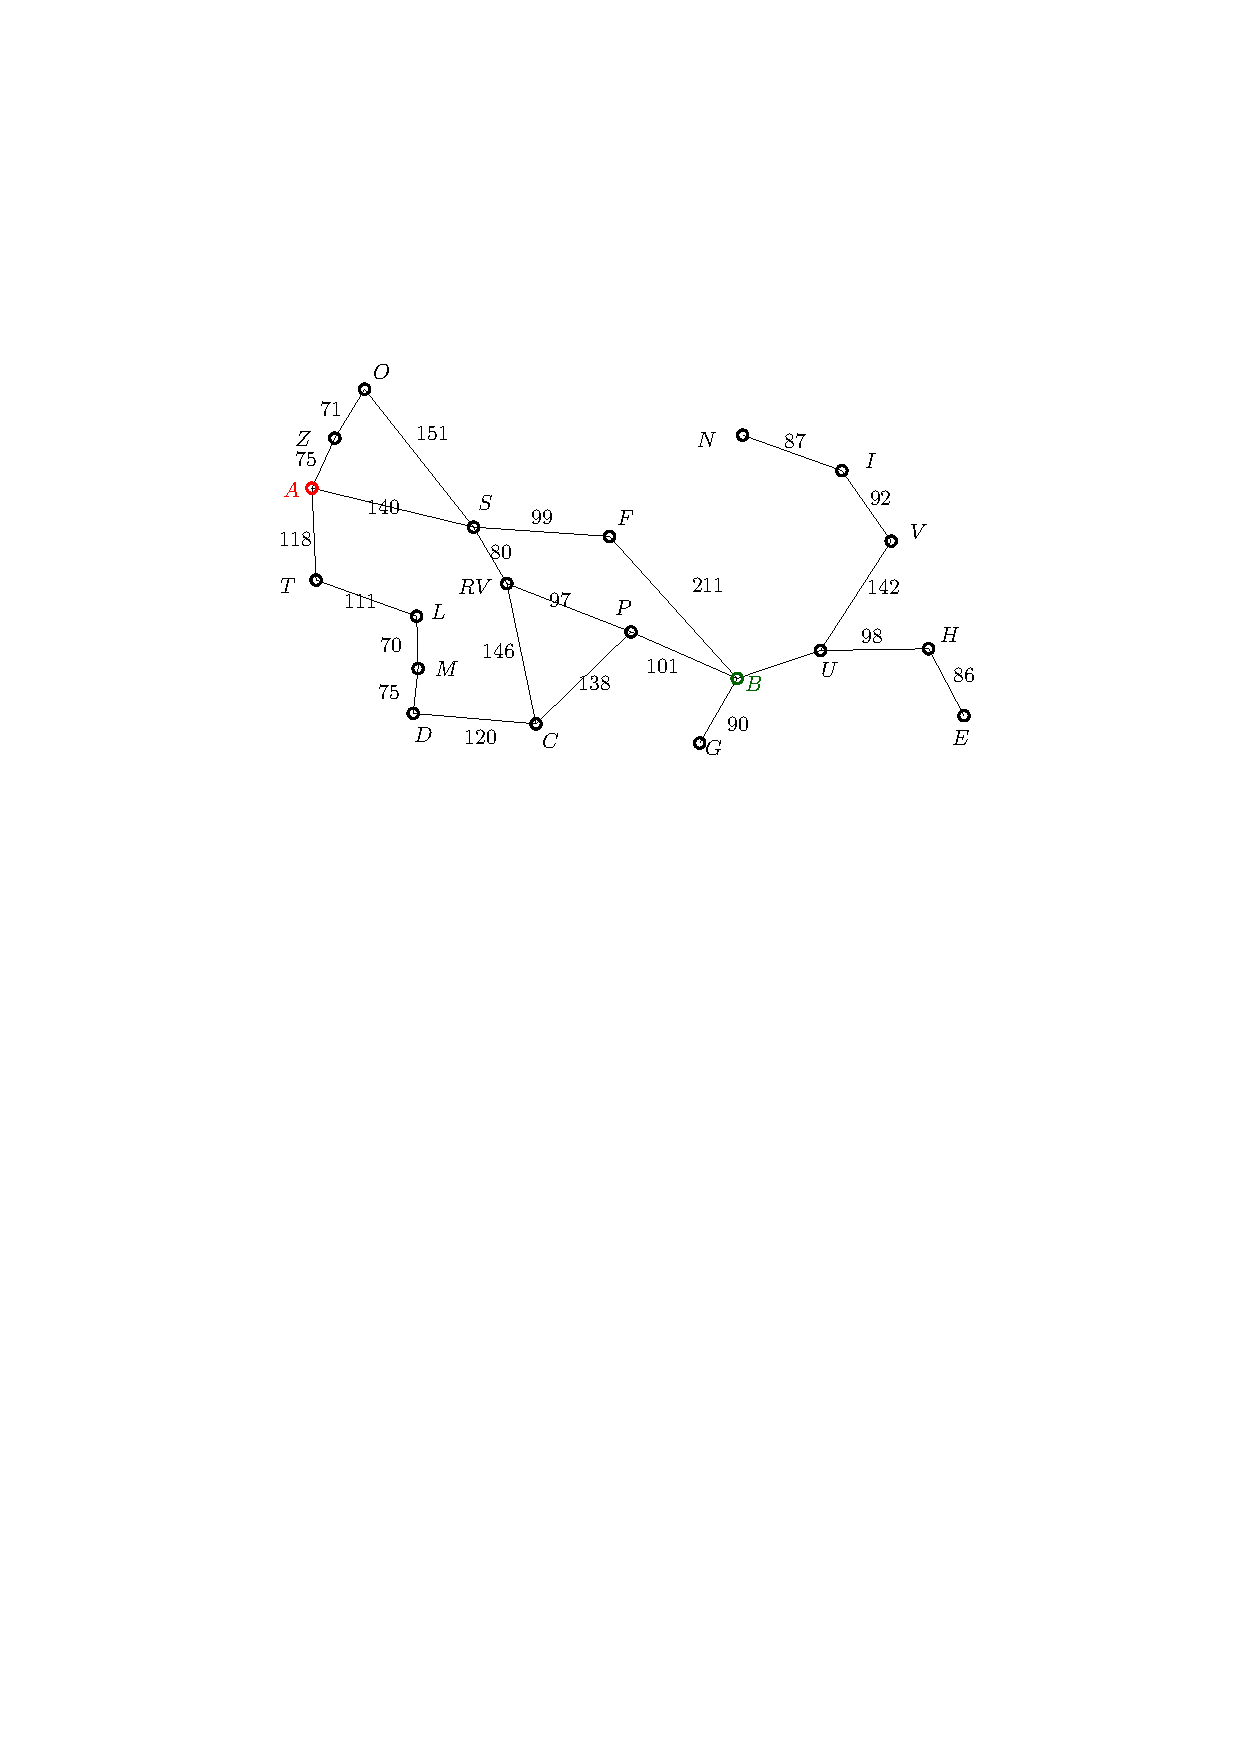
\includegraphics{image/评价函数例题.pdf}
    \end{figure}
    \begin{enumerate}
        \item 一致代价图搜索
        
        \textcolor{main1}{解序列:}$A\to S\to RV\to P\to B$

        \textcolor{main1}{解代价:}408
        % Table generated by Excel2LaTeX from sheet '一致代价搜索'
        \begin{table}[htbp]
            \centering
            \begin{tabular}{cc}
            \toprule[1.5pt]
            Step & frontier \\
            \midrule[1pt]
            Step 1 & $A(0)$ \\
            Step 2 & $Z(75),\,T(118),\,S(140)$ \\
            Step 3 & $T(118),\,S(140),\,O(146)$ \\
            Step 4 & $S(140),\,O(146),\,L(229)$ \\
            Step 5 & $O(146),\,RV(220),\,L(229),\,F(239)$ \\
            Step 6 & $RV(220),\,L(229),\,F(239)$ \\
            Step 7 & $L(229),\,F(239),\,P(317),\,C(366)$ \\
            Step 8 & $F(239),\,M(299),\,P(317),\,C(366)$ \\
            Step 9 & $M(299),\,P(317),\,C(366),\,B(450)$ \\
            Step 10 & $P(317),\,C(366),\,D(374),\,B(450)$ \\
            Step 11 & $C(366),\,D(374),\,B(408)$ \\
            Step 12 & $D(374),\,B(408)$ \\
            Step 13 & $B(408)$ \\
            \bottomrule[1.5pt]
            \end{tabular}%
        \end{table}%
        \item 贪婪搜索
                
        \textcolor{main1}{解序列:}$A\to S\to F\to B$

        \textcolor{main1}{解代价:}450
        \begin{figure}[H]
            \centering
            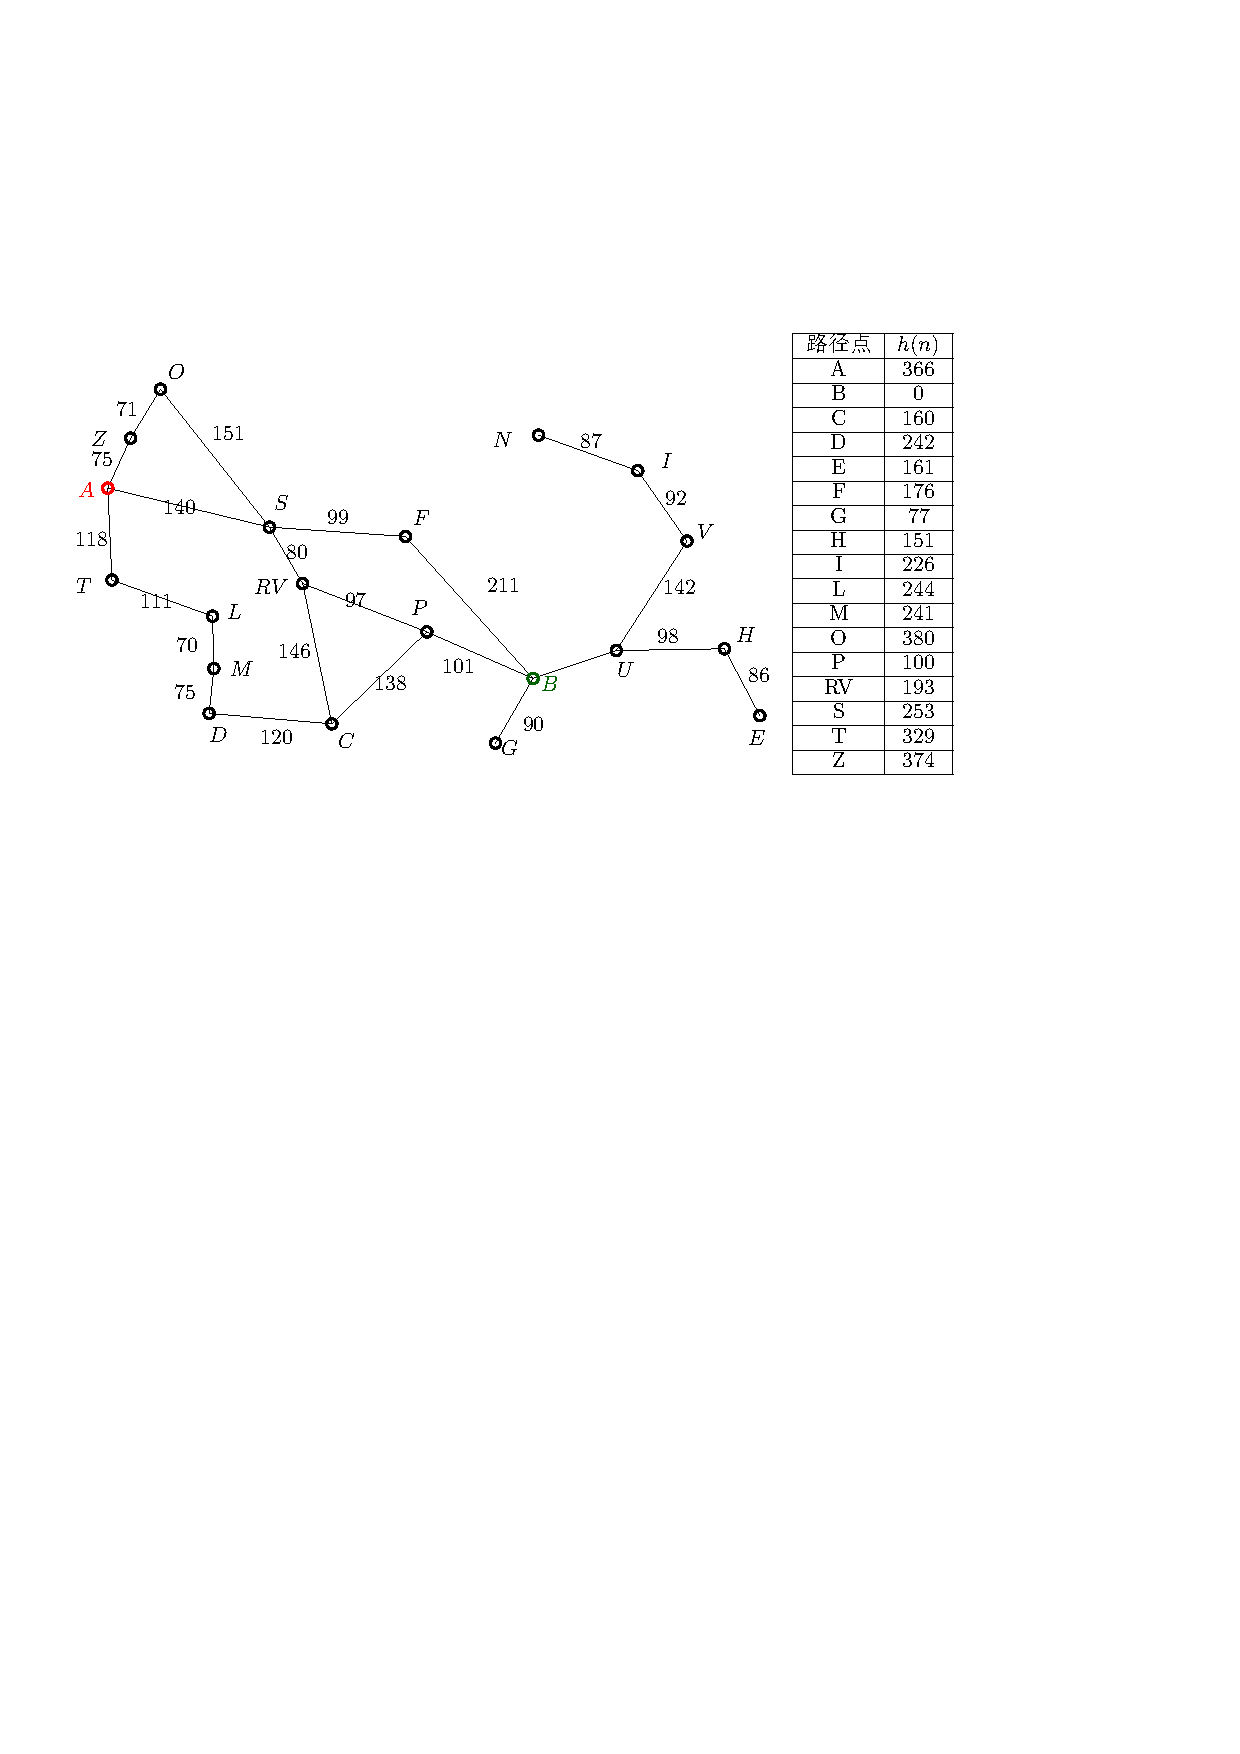
\includegraphics[width = \textwidth]{image/评价函数例题-1.pdf}
        \end{figure}
        % Table generated by Excel2LaTeX from sheet '贪婪搜索 (2)'
        \begin{table}[htbp]
            \centering
            \begin{tabular}{ccc}
            \toprule[1.5pt]
            Step & frontier & explored \bigstrut\\
            \midrule[1pt]
            Step 1 & $A(366)$ &  \bigstrut[t]\\
            Step 2 & $S(253),\,T(329),\,Z(374)$ & $A$ \\
            Step 3 & $F(176),\,RV(193),\,T(329),\,Z(374),\,O(380)$ & $A,\,S$ \\
            Step 4 & $B(0),\,RV(193),\,T(329),\,Z(374),\,O(380)$ & $A,\,S,\,F$ \bigstrut[b]\\
            \bottomrule[1.5pt]
            \end{tabular}%
        \end{table}%
        \item A\textsuperscript{*}搜索
        
        \textcolor{main1}{解序列:}$A\to S\to RV\to P\to B$

        \textcolor{main1}{解代价:}408
        % Table generated by Excel2LaTeX from sheet 'A-Star'
        \begin{table}[htbp]
            \centering
            \begin{tabular}{ccc}
            \toprule[1.5pt]
            Step & frontier & explored \\
            \midrule[1pt]
            Step 1 & $A(366)$ &  \\
            Step 2 & $S(393),\,T(447),\,Z(449)$ & $A$ \\
            Step 3 & $RV(413),\,F(415),\,T(447),\,Z(449),\,O(671)$ & $A,\,S$ \\
            Step 4 & $F(415),\,P(417),\,T(447),\,Z(449),\,C(526),\,O(671)$ & $A,\,S,\,RV$ \\
            Step 5 & $P(417),\,T(447),\,Z(449),\,B(450),\,C(526),\,O(671)$ & $A,\,S,\,RV,\,F$ \\
            Step 6 & $B(408),\,T(447),\,Z(449),\,C(526),\,O(671)$ & $A,\,S,\,RV,\,F,\,P$ \\
            \bottomrule[1.5pt]
            \end{tabular}%
        \end{table}%
    \end{enumerate}
\end{example}
\begin{example}
    $S$为初始状态,$G_1$和$G_2$为目标状态。各状态之间的代价已标注在连接两个状态的连线上 (注意连线是有方向的),每个状态到达目标的估计代价标注在其内部。分别应用\textcolor{main1}{一致代价、贪婪、A\textsuperscript{*}搜索策略},指出图搜索算法将会到达的目标状态($G_1$或$G_2$),并按顺序写出搜索过程中所考察的节点。在其他条件都相同的情况下,按照字母先后顺序对节点进行扩展。
    \begin{figure}[htbp]
        \centering
        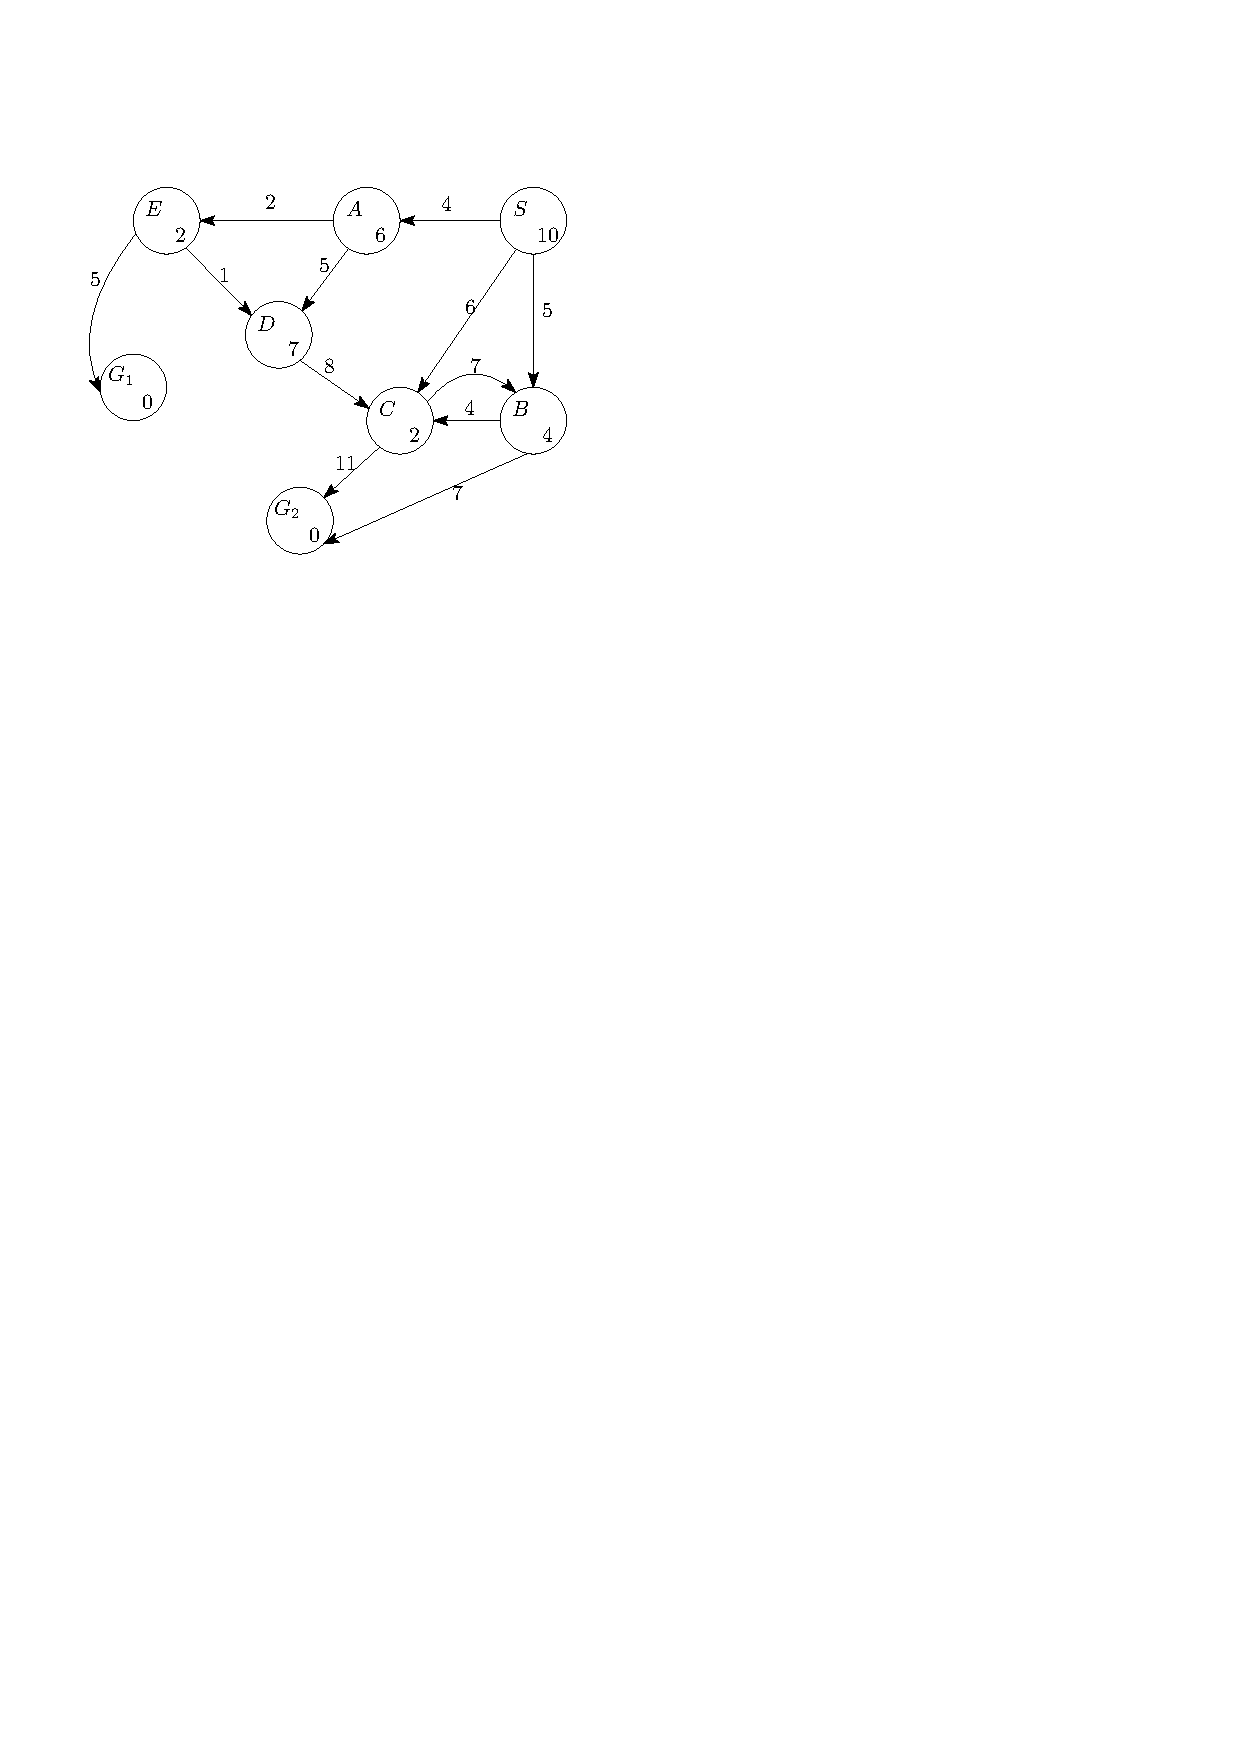
\includegraphics{image/搜索策略例题.pdf}
    \end{figure}
    \begin{enumerate}
        \item 一致代价
        
        \textcolor{main1}{解序列:}$S\to A\to E\to G_1$

        \textcolor{main1}{解代价:}11
        % Table generated by Excel2LaTeX from sheet '一致代价搜索'
        \begin{table}[htbp]
            \centering
            \begin{tabular}{ccc}
            \toprule[1.5pt]
            Step & frontier & explored \\
            \midrule[1pt]
            Step 1 & $S(0)$ &  \\
            Step 2 & $A(4),\,B(5),\,C(6)$ & $S$ \\
            Step 3 & $B(5),\,C(6),\,E(6),\,D(9)$ & $S,\,A$ \\
            Step 4 & $C(6),\,E(6),\,D(9),\,G_2(12)$ & $S,\,A,\,B$ \\
            Step 5 & $E(6),\,D(9),\,G_2(12)$ & $S,\,A,\,B,\,C$ \\
            Step 6 & $D(7),\,G_1(11),\,G_2(12)$ & $S,\,A,\,B,\,C,\,E$ \\
            Step 7 & $G_1(11),\,G_2(12)$ & $S,\,A,\,B,\,C,\,E,\,D$ \\
            \bottomrule[1.5pt]
            \end{tabular}%
        \end{table}%  
        \item 贪婪
                
        \textcolor{main1}{解序列:}$S\to C\to G_2$

        \textcolor{main1}{解代价:}17
        % Table generated by Excel2LaTeX from sheet '贪婪搜索 (2)'
        \begin{table}[htbp]
            \centering
            \begin{tabular}{ccc}
            \toprule[1.5pt]
            Step & frontier & explored \\
            \midrule[1pt]
            Step 1 & $S(0)$ &  \\
            Step 2 & $C(2),\,B(4),\,A(6)$ & $S$ \\
            Step 4 & $G_2(0),\,B(4),\,A(6)$ & $S,\,C$ \\
            \bottomrule[1.5pt]
            \end{tabular}%
        \end{table}%
        \item A\textsuperscript{*}
                        
        \textcolor{main1}{解序列:}$S\to A\to E\to G_1$

        \textcolor{main1}{解代价:}11
        % Table generated by Excel2LaTeX from sheet 'A-Star'
        \begin{table}[htbp]
            \centering
            \begin{tabular}{ccc}
            \toprule
            Step & frontier & explored \\
            \midrule
            Step 1 & $S(10)$ &  \\
            Step 2 & $C(8),\,B(9),\,A(10)$ & $S$ \\
            Step 3 & $B(9),\,A(10),\,G_2(12)$ & $S,\,C$ \\
            Step 4 & $A(10),\,G_2(12)$ & $S,\,C,\,B$ \\
            Step 5 & $E(8),\,G_2(12),\,D(16)$ & $S,\,C,\,B,\,A$ \\
            Step 6 & $G_1(11),\,G_2(12),\,D(14)$ & $S,\,C,\,B,\,A,\,E$ \\
            \bottomrule
            \end{tabular}%
        \end{table}%
    
    \end{enumerate}
\end{example}
\subsection{博弈树搜索}
\subsubsection{博弈问题}
\begin{definition}[博弈]
    在一定条件下,遵守一定的\textcolor{main1}{规则},\textcolor{main1}{一个或几个}拥有绝对理性思维的人或团队,从各自允许选择的行为或策略中选择并加以实施,并从中各自取得相应\textcolor{main1}{结果或收益}的过程。
\end{definition}
\begin{definition}[双方信息完备的零和博弈]
    包括以下内容:\newline
    \begin{itemize}
        \item 对抗的双方
        
        双方参与者轮流采取行动,选取对自己最有利而对对方最不利的对策
        \item 双方信息完备的零和博弈
        
        任何一方都了解当前的格局及过去的历史
        \item 零和
        
        参与者的利益严格对立,双方得失之和为零
    \end{itemize} 
\end{definition}

\begin{note}
    \textcolor{main1}{信息完备:}
    已知对方走过的棋步以及当前的局面。

    \textcolor{main1}{信息不完备:}
    参与人并不完全清楚对手的情况,只能进行估计。
\end{note}

\begin{example}
    下面哪些属于双方信息完备的零和博弈:
    \begin{enumerate}[A.]
        \item \textcolor{main1}{五子棋}
        \item 桥牌
        \item \textcolor{main1}{中国象棋}
        \item \textcolor{main1}{足球}
        \item \textcolor{main1}{围棋}
        \item 中美经济博弈
    \end{enumerate}
\end{example}

博弈问题分析的关键要素:
\begin{enumerate}
    \item 状态:棋盘上棋子位置布局
    \item 动作:各类棋子合法走步
    \item 开局/终局:游戏开始/结束的状态
    \item 终局效用值:终局下某个棋手的效用值
    \item 状态空间:合法动作作用于当前状态生成的博弈树
    \item 某个玩家的\textcolor{main1}{解}为一个\textcolor{main1}{策略}: 状态$\to $动作
\end{enumerate}
\subsubsection{minimax搜索算法}
极小极大搜索算法(三个阶段)
\begin{enumerate}
    \item 生成规定深度的全部博弈树,计算所有最底层节点的静态估计函数值
    \item 自底向上逐层计算非终结节点的倒推估计值
    \begin{itemize}
        \item 对于MAX层节点,取其所有子节点的最大值
        \item 对于MIN层节点,取其所有子节点的最小值
    \end{itemize}
    \item 标记最佳走步:
    \begin{itemize}
        \item 对于MAX选手,选择使其$f$值最大的走步
        \item 对于MIN选手,选择使其$f$值最小的走步
    \end{itemize}
\end{enumerate}

算法性质分析:
\begin{figure}[htbp]
    \centering
    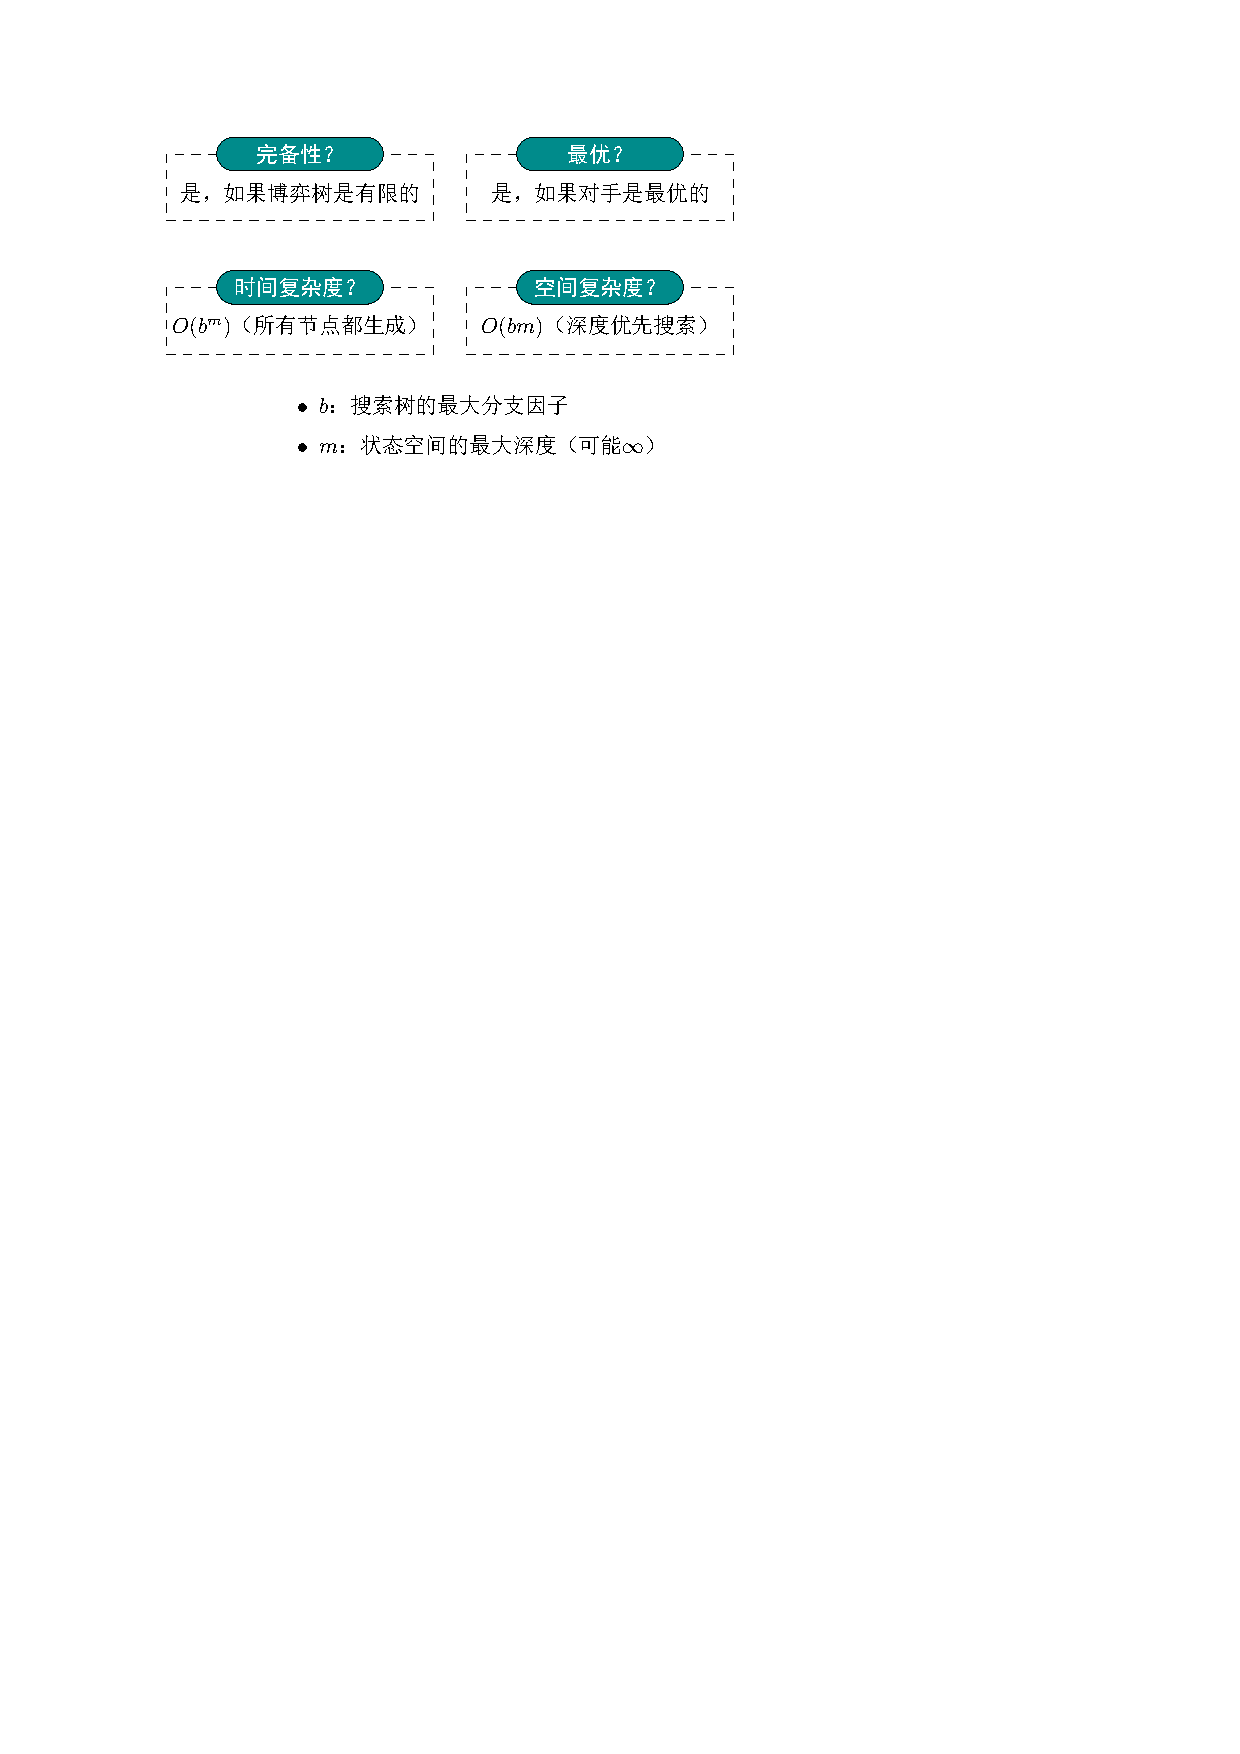
\includegraphics{image/minmax性质.pdf}
\end{figure}
\begin{note}
    博弈树的规模一般都很大
    \begin{itemize}
        \item 国际象棋:走10个会合后,总节点数量级$10^{31}$
        \item 中国象棋:走10个会合后,总节点数量级$10^{32}$
        \item 围棋:走10个回合后,总节点数量级$10^{51}$
    \end{itemize}
\end{note}
极大极小搜索过程存在的问题
由于要\textcolor{main1}{生成置顶深度以内的所有节点},其节点数将随着搜索深度的增加成指数增长。
\subsubsection{\texorpdfstring{$\alpha-\beta$}{α-β}剪枝}

\begin{note}
    进行$\alpha-\beta$剪枝时,应注意的问题
    \begin{itemize}
        \item 应\textcolor{main1}{相邻层比较}(MAX节点和MIN节点间),不能进行同层比较
        \item 至少一个子节点的推导值\textcolor{main1}{固定以后},才能向父节点传递
        \item 在实际搜索时,不能按宽度优先建立搜索树,再进行剪枝,而是按照\textcolor{main1}{有界深度优先搜索}的方式生成节点,\textcolor{main1}{边生成边剪枝}。
    \end{itemize}
\end{note}
\begin{note}
    特性分析
    \begin{itemize}
        \item $\alpha-\beta$剪枝对计算根节点的MiniMax值没有影响
        \item 剪枝效率最坏情况$O(b^m)$(其中$b$是分支数,$m$是解的深度)
        \item 剪枝效率最好情况$O(b^{m/2})$
        \begin{itemize}
            \item 不管是MAX选手还是MIN选手,最好选择都是博弈树的最左分枝,存在较多的剪枝。
        \end{itemize}
    \end{itemize}
\end{note}
\begin{example}
    对下面的博弈树按从左到右的顺序进行$\alpha-\beta$剪枝搜索,试标明各生成节点的倒推值,何处发生剪枝及应选择的走步。
    \begin{figure}[htbp]
        \centering
        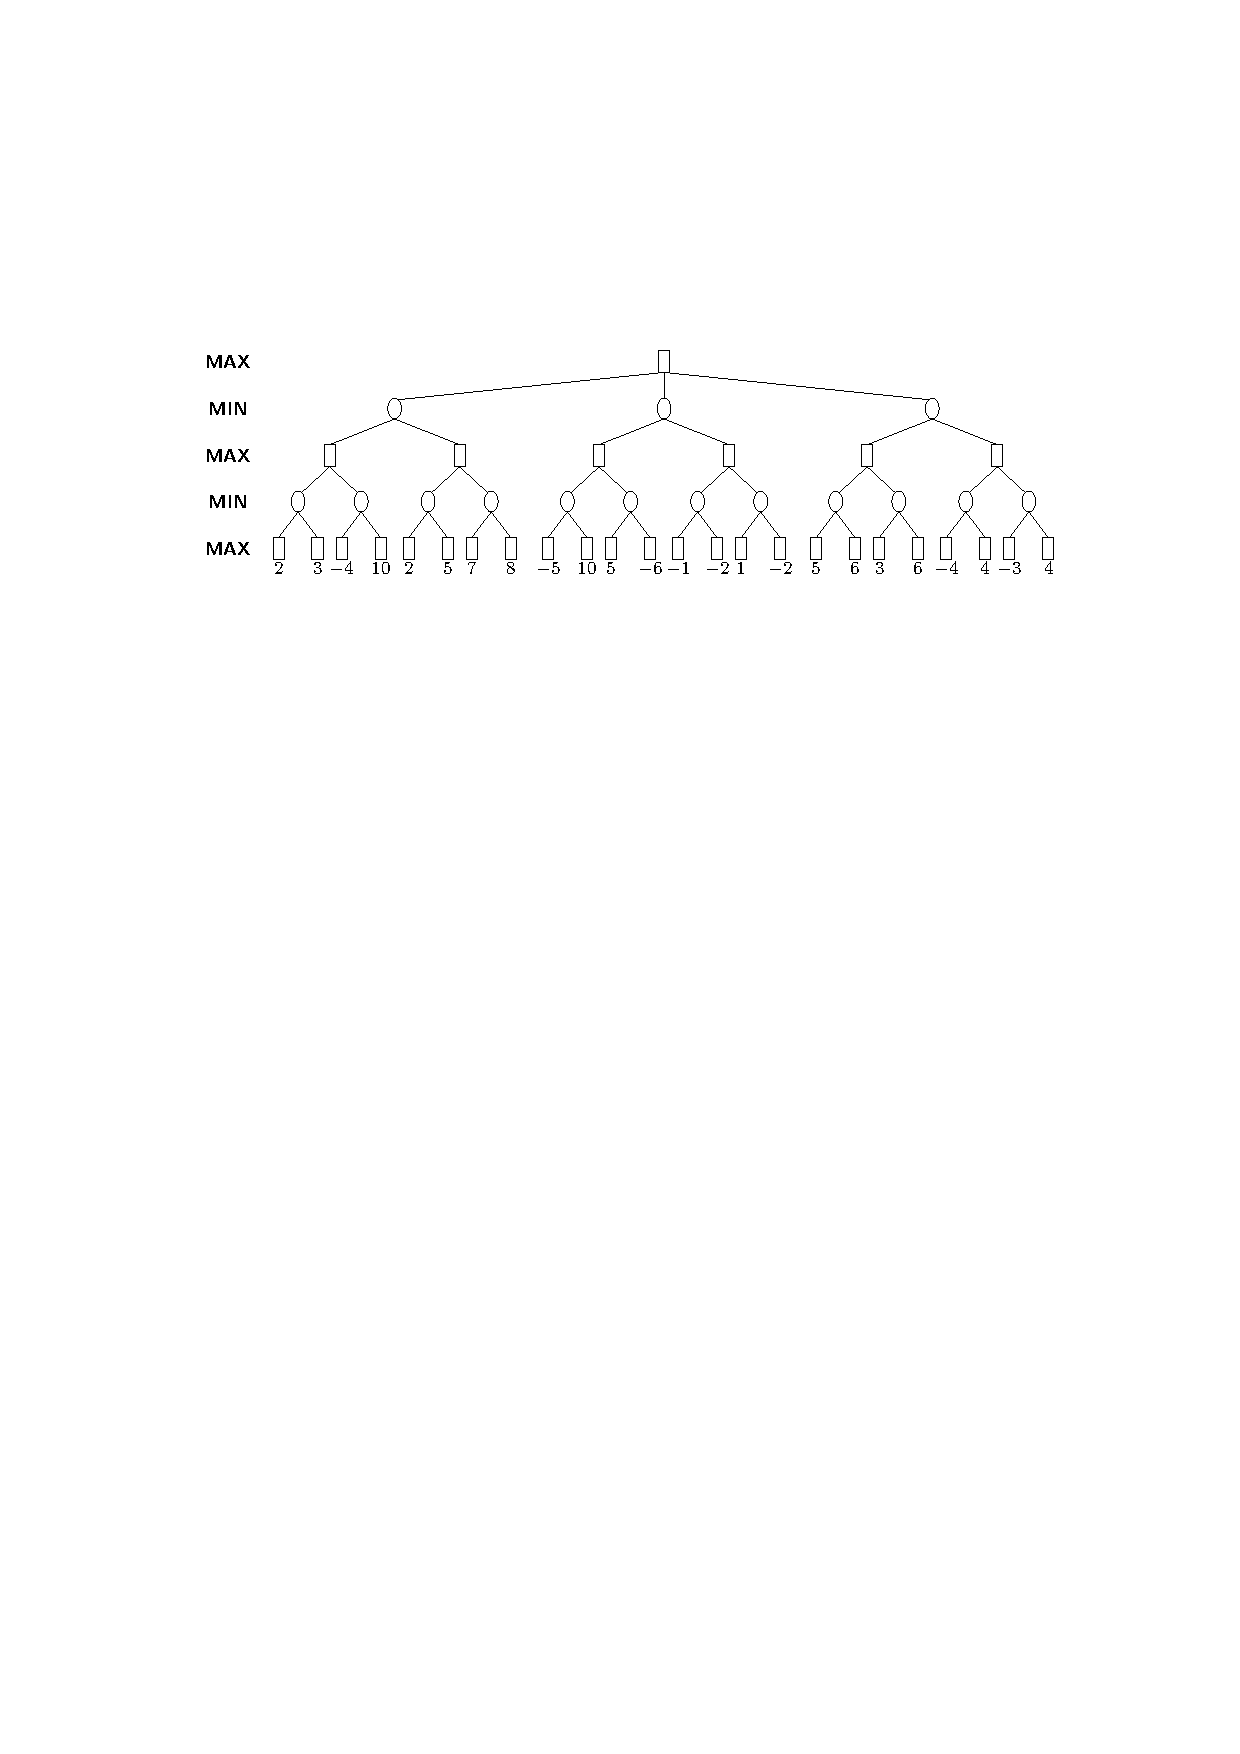
\includegraphics[width = .86\textwidth]{image/alpha-beta.pdf}
    \end{figure}

    \begin{figure}[htbp]
        \centering
        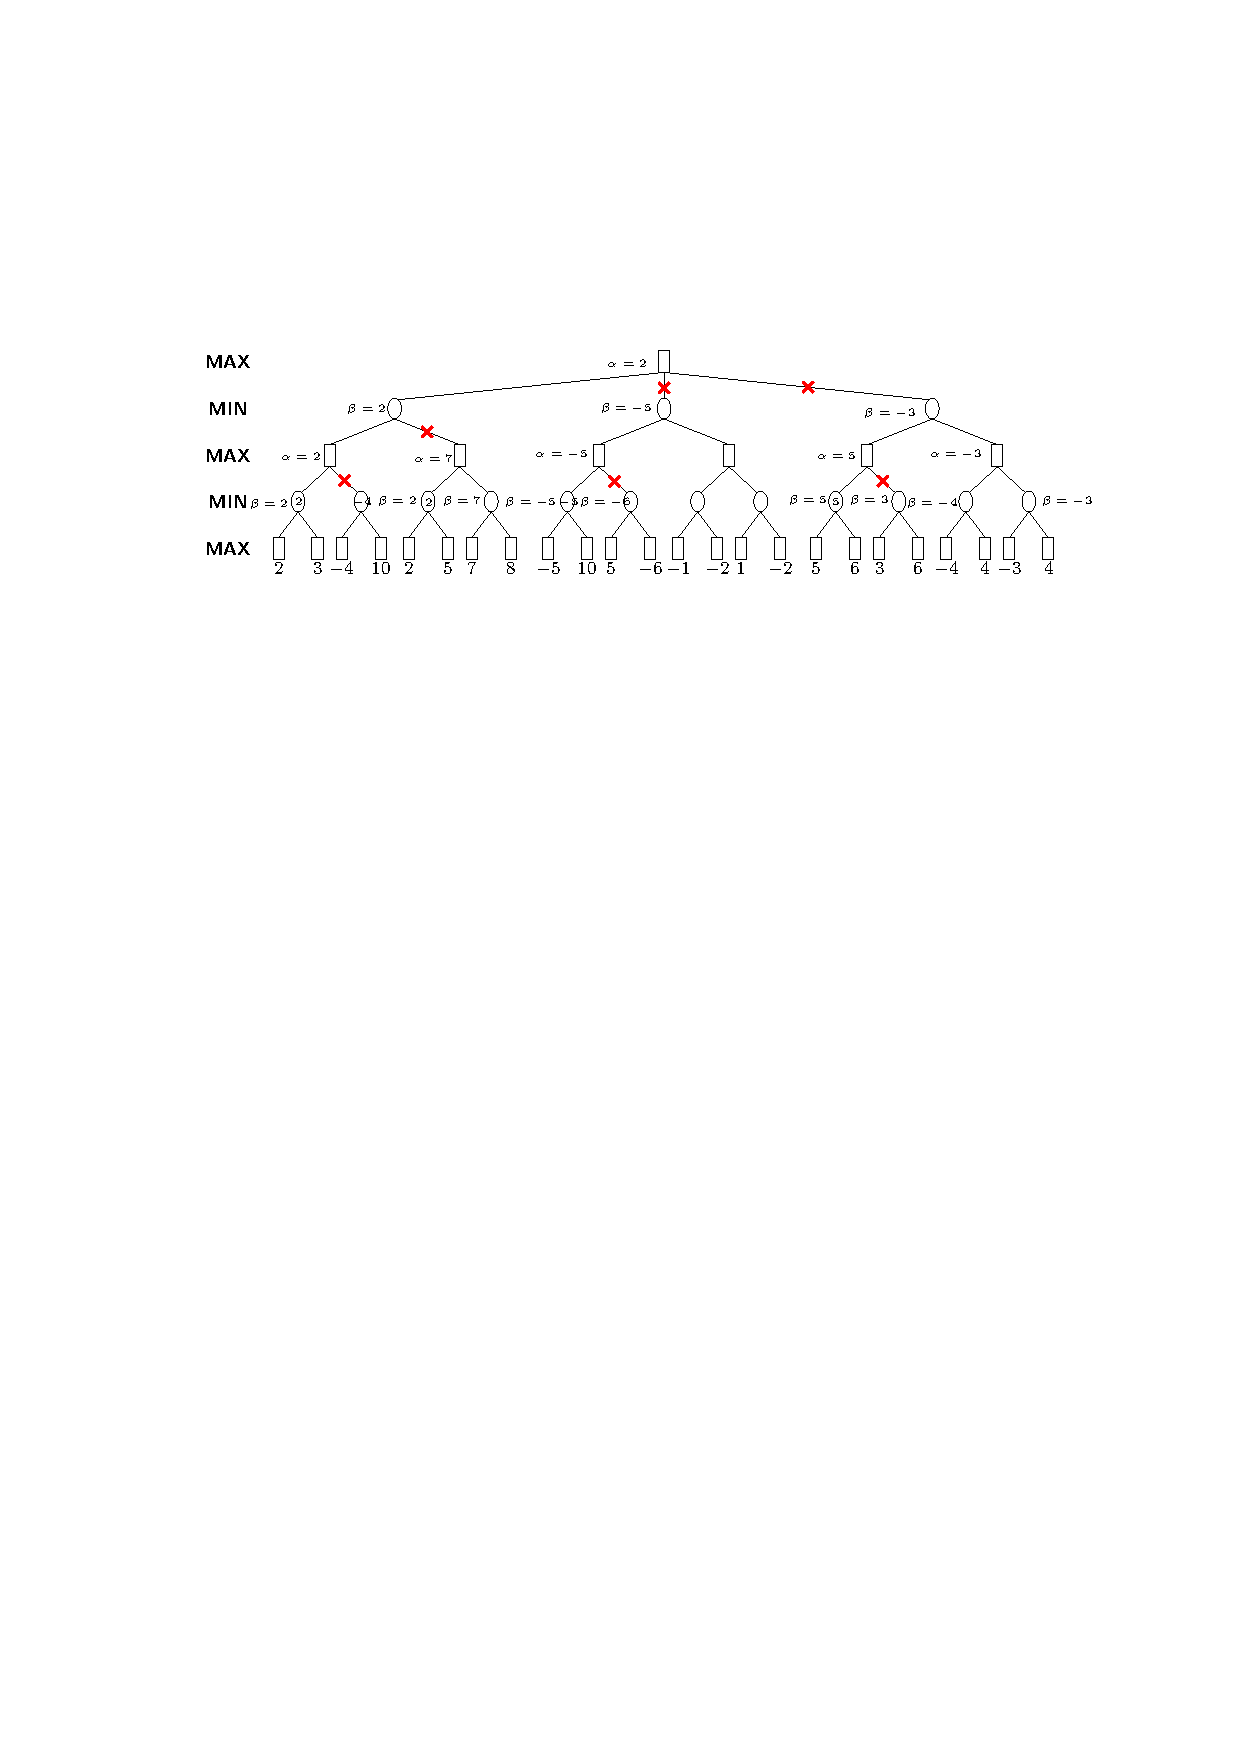
\includegraphics[width = .86\textwidth]{image/alpha-beta-sol.pdf}
    \end{figure}
\end{example}
\section{知识表示与推理}
\subsection{逻辑Agent}
\subsubsection{基于知识的Agent}

\begin{figure}[htbp]
    \centering
    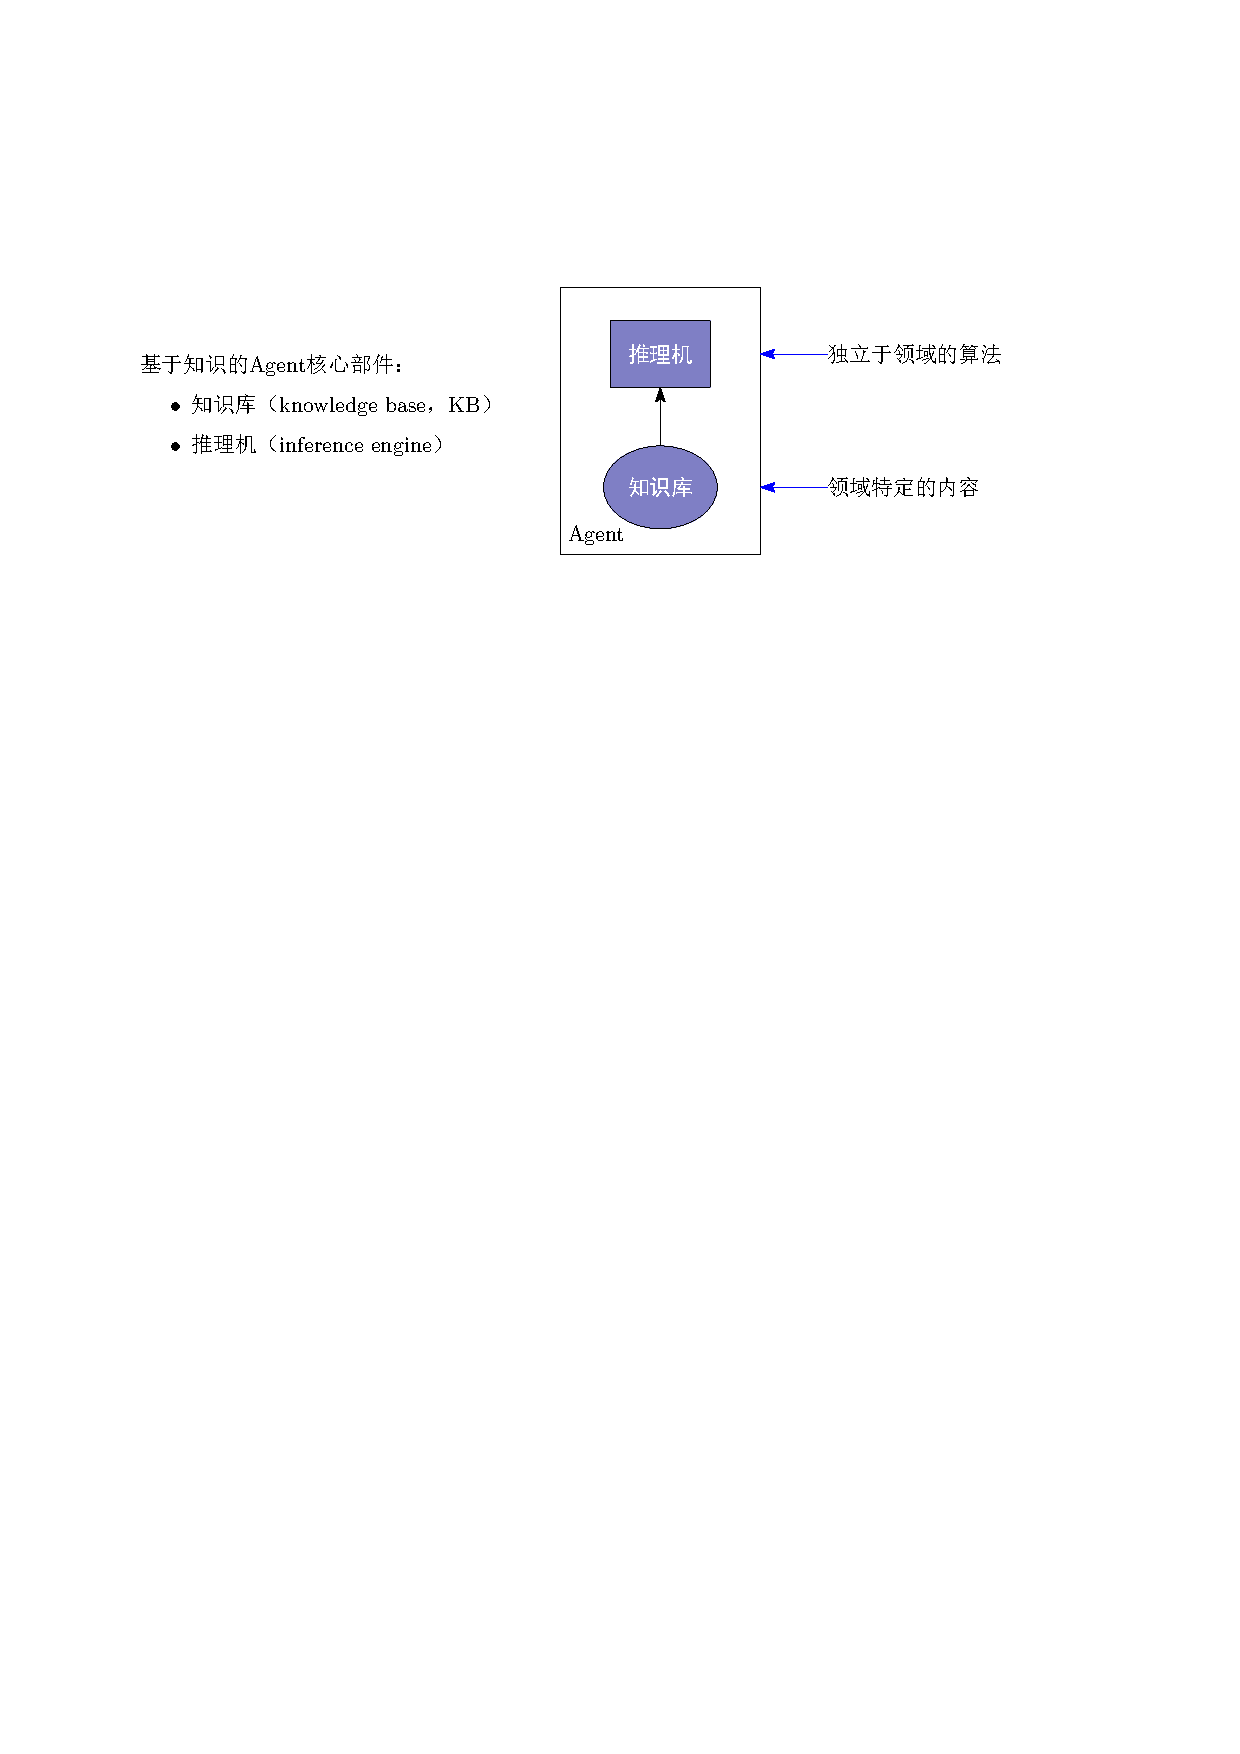
\includegraphics{image/基于知识的Agent.pdf}
\end{figure}

\begin{definition}[蕴含(Entailment)]
    知识库KB(一组对已知世界和规则描述的逻辑语句)蕴含语句$\alpha$(某个待确定的逻辑结论),当且仅当在KB为真的所有世界中$\alpha$也为真。蕴含表示为
    \[
        \textcolor{main1}{KB}\models\alpha 
    \]
    即,若$\textcolor{main1}{KB}\models\alpha $,当且仅当$M(KB)\subseteq M(\alpha)$
\end{definition}
\subsubsection{命题逻辑的推理}
\begin{figure}[htbp]
    \centering
    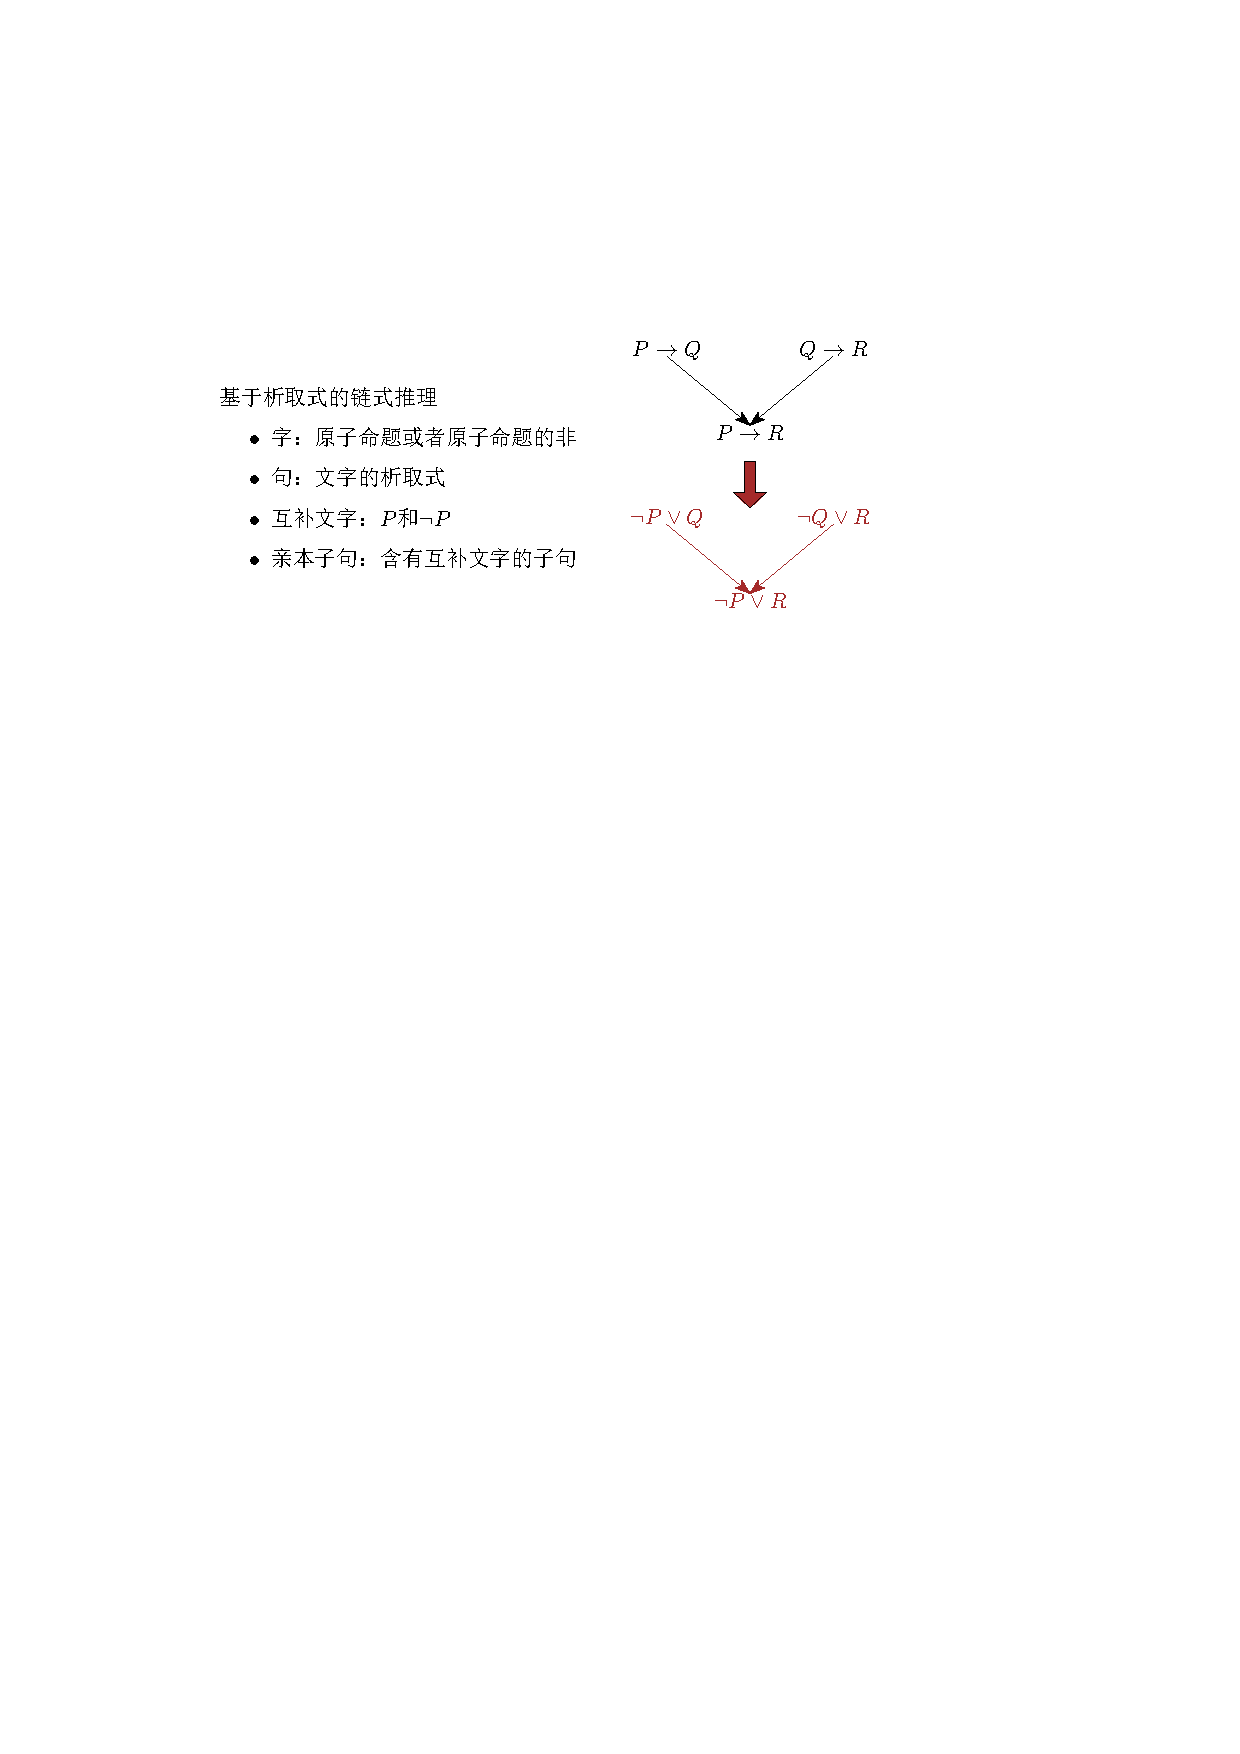
\includegraphics{image/基于析取式的链式推理.pdf}
\end{figure}
\begin{note}
    归结(Resolution):

    链式推理和假言推理都可以转化成相同的推理规则:\textcolor{main1}{两个含有互补文字的亲本子句可以进行推理,推理得到的结论是去除互补文字后两个子句的析取式。}
\end{note}
\begin{definition}[析取范式]
    设$A$为如下形式的命题公式$B_1\lor B_2\lor \dots\lor B_n$,其中$B_i,\ (i = 1,2,\dots, n)$为原子命题或其否定,则$A$称为析取范式或析取式。
\end{definition}
\begin{note}
    归结中需要注意的问题1:
    \begin{itemize}
        \item 进行归结之前,需要把已知的事实、定理等化成\textcolor{main1}{析取范式或者是单个文字的形式,}单个文字是原子命题,也可以看成一个析取范式。
        \item \textcolor{main1}{析取范式之间的逻辑关系是合取},也就是“与”因为子句表示的是已知事实或者定理,这些子句必须同时成立才能推导出结论。
    \end{itemize}
    子句间是合取关系,子句内是析取形式。
\end{note}
\begin{example}
    选取两个含有互补文字的子句进行归结,产生新的子句,如果新子句和原始子句含有互补文字,那么继续归结,直到再没有亲本子句。
    \begin{figure}[htbp]
        \centering
        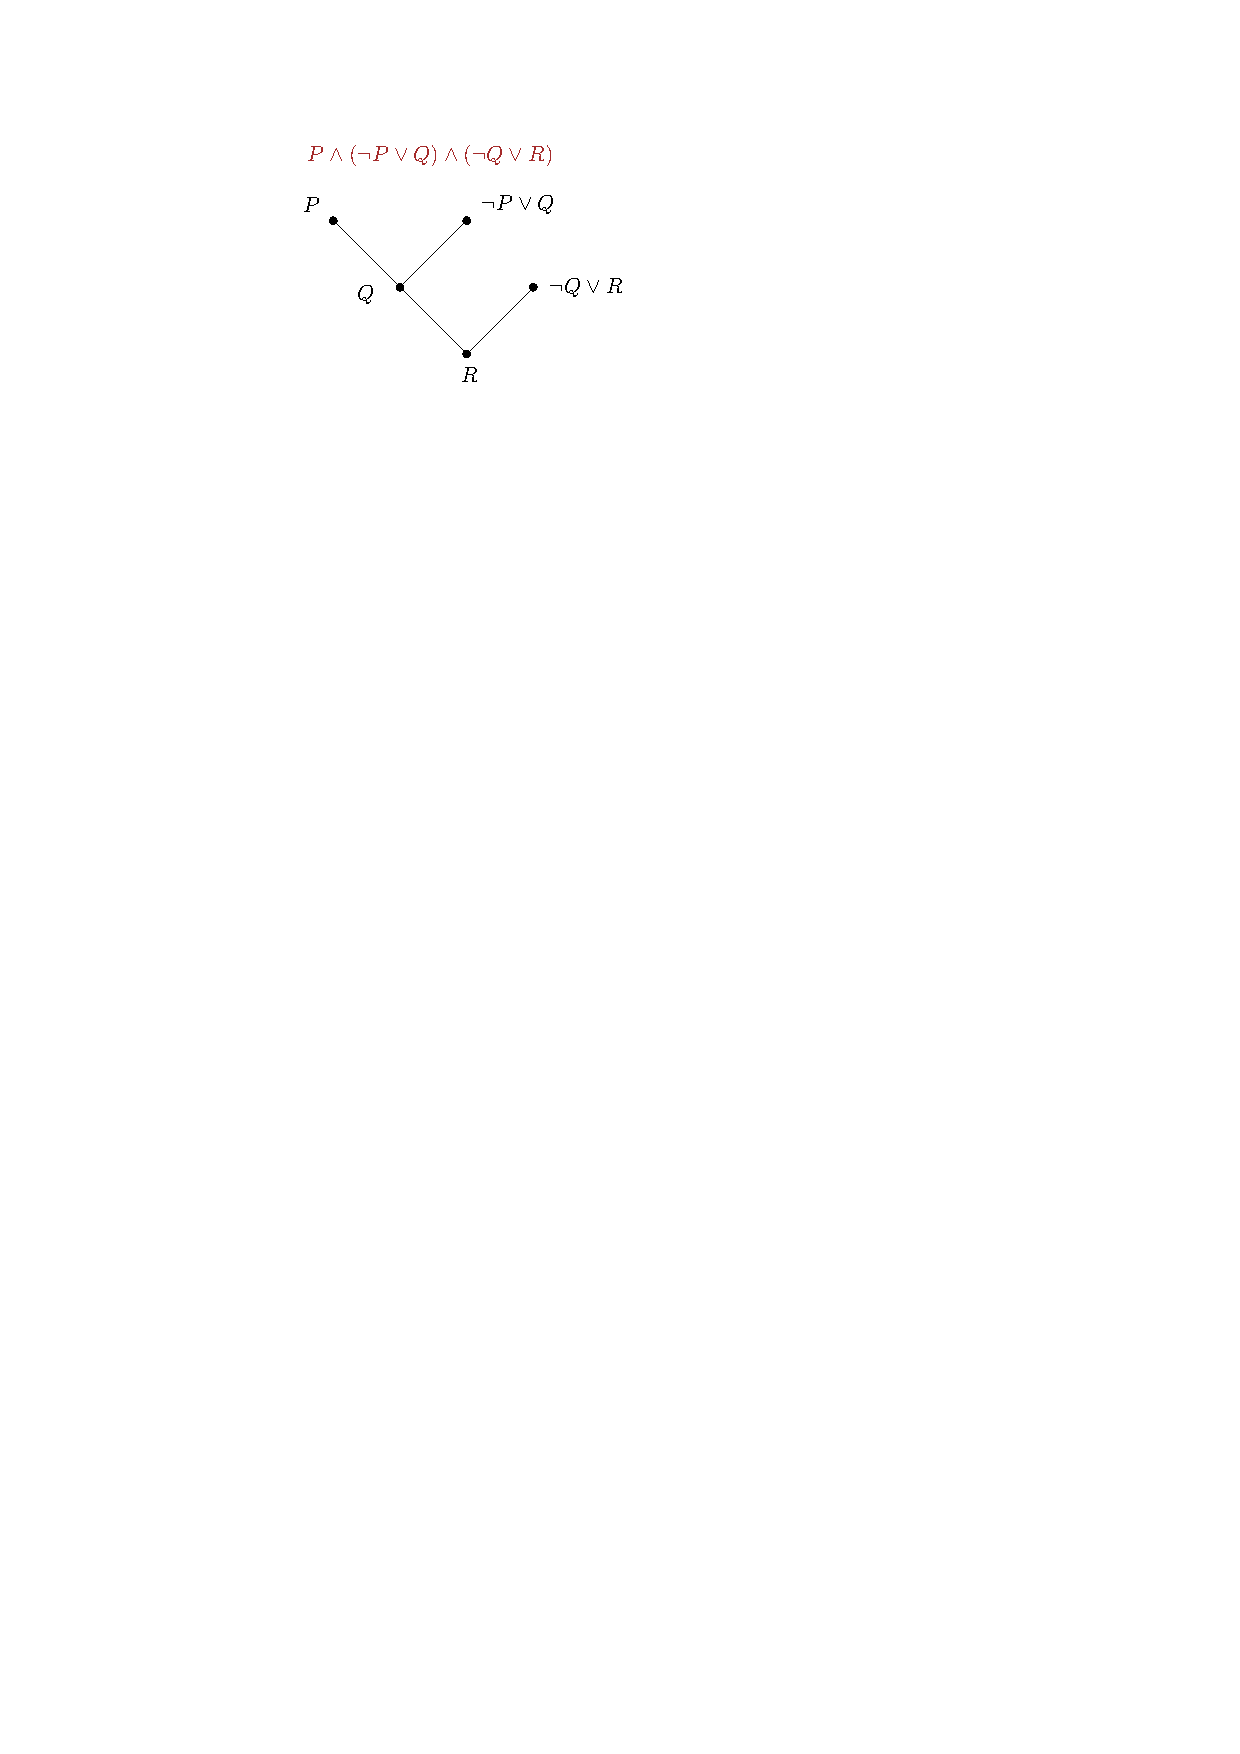
\includegraphics{image/归结.pdf}
    \end{figure}
\end{example}
\begin{example}
    将以下问题进行归结:
    \begin{enumerate}
        \item 将$\lnot P\lor Q\lor W$与$P\lor Q\lor R\lor S$归结。
        \begin{figure}[htbp]
            \centering
            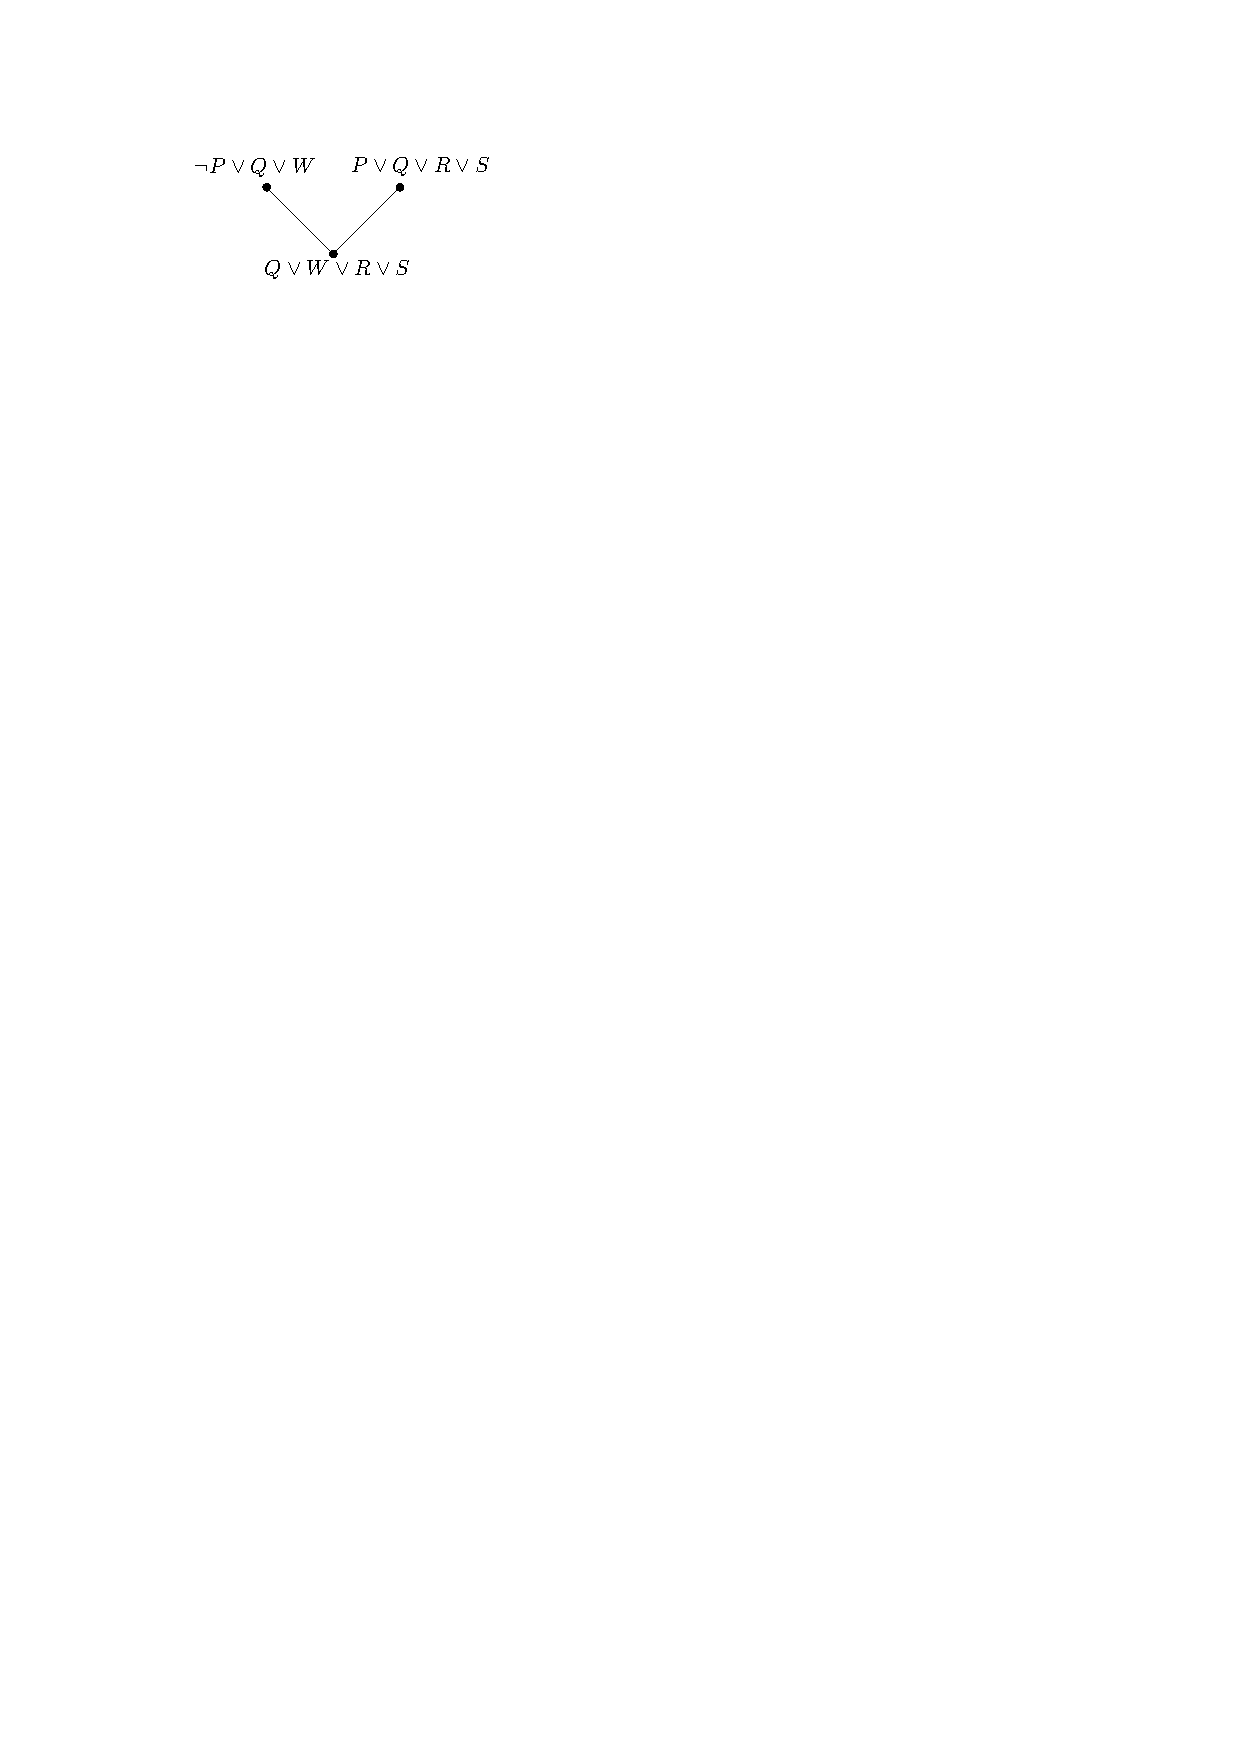
\includegraphics{image/归结-1.pdf}
        \end{figure}
        \item $P\lor W\lor \lnot Q\lor R$与$P\lor Q\lor \lnot R$归结的结果是什么?
        \begin{figure}[htbp]
            \centering
            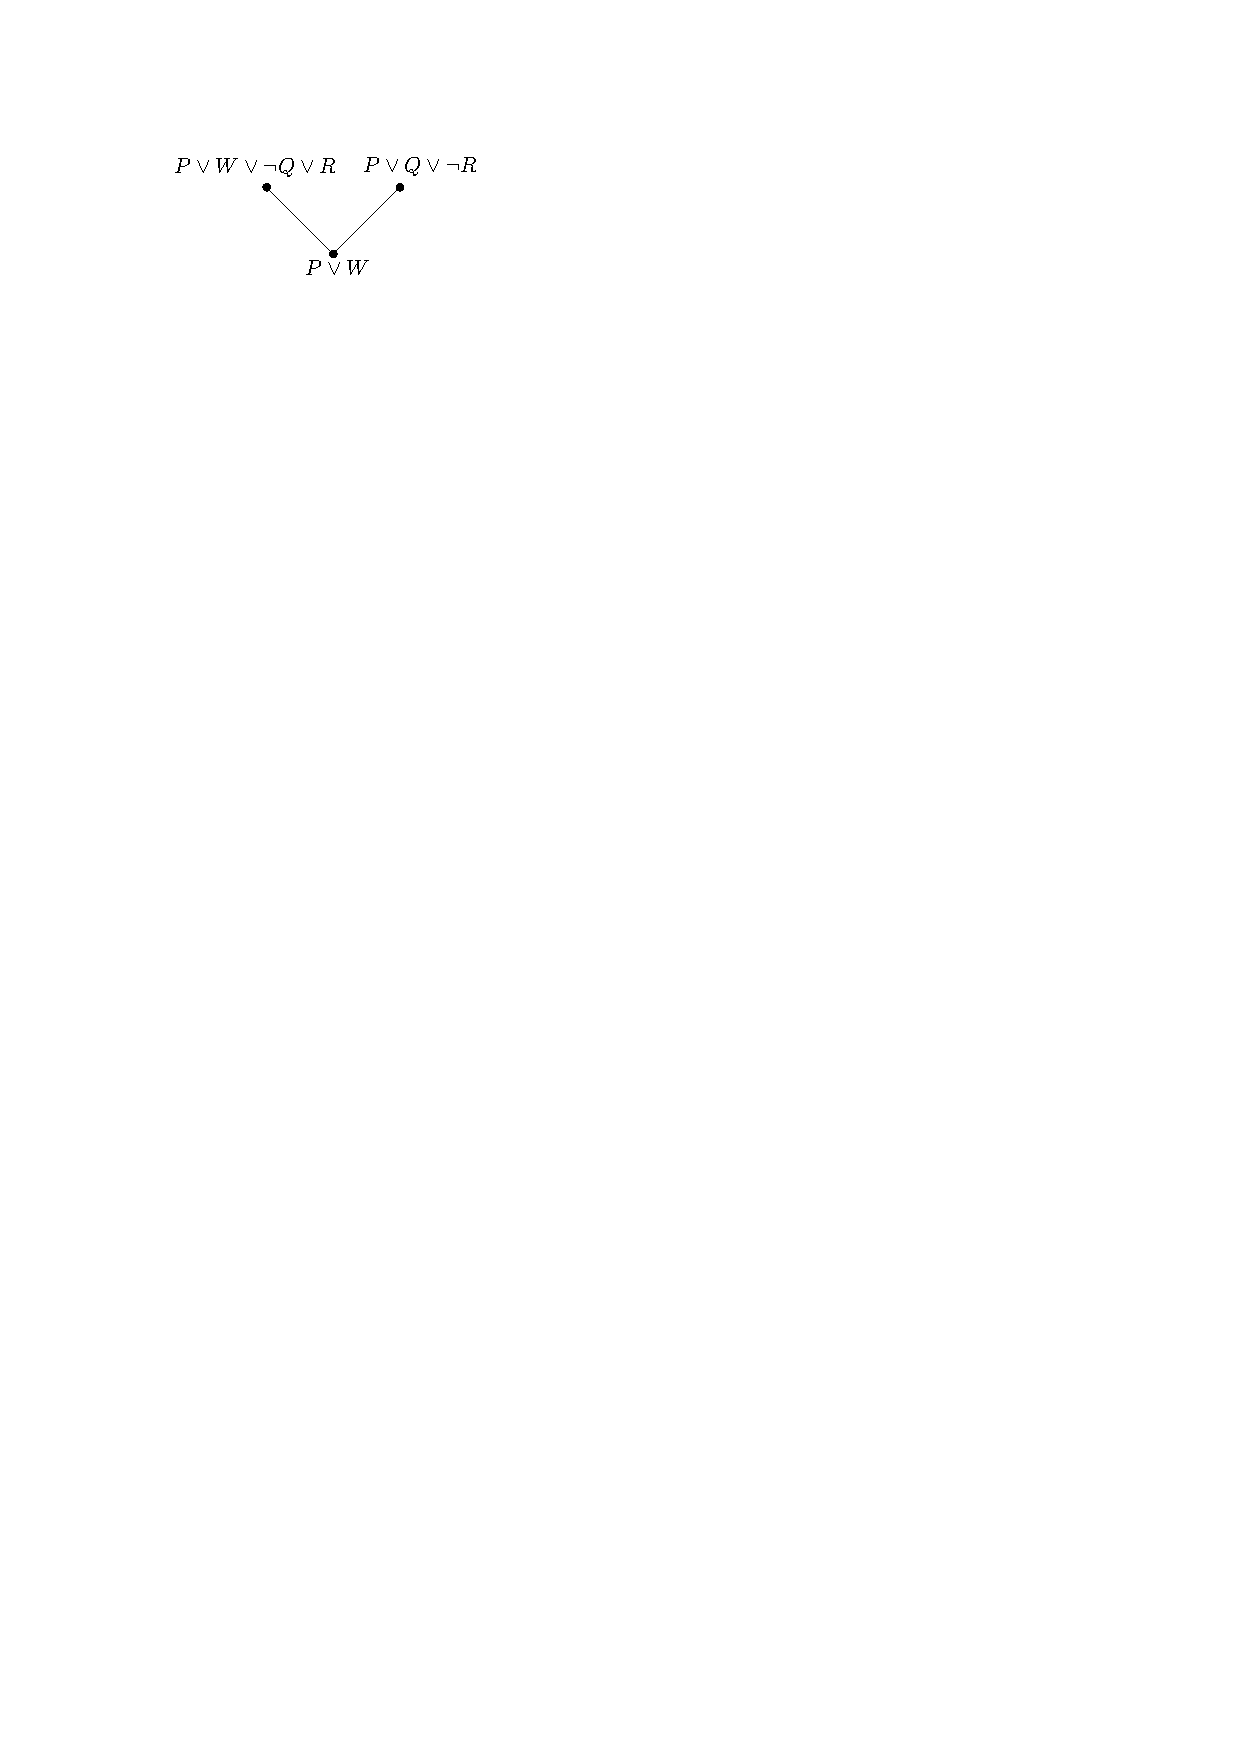
\includegraphics{image/归结-2.pdf}
        \end{figure}
        \item 将$P\lor \lnot Q$与$P\lor Q$以及$\lnot P$归结
        \begin{figure}[!h]
            \centering
            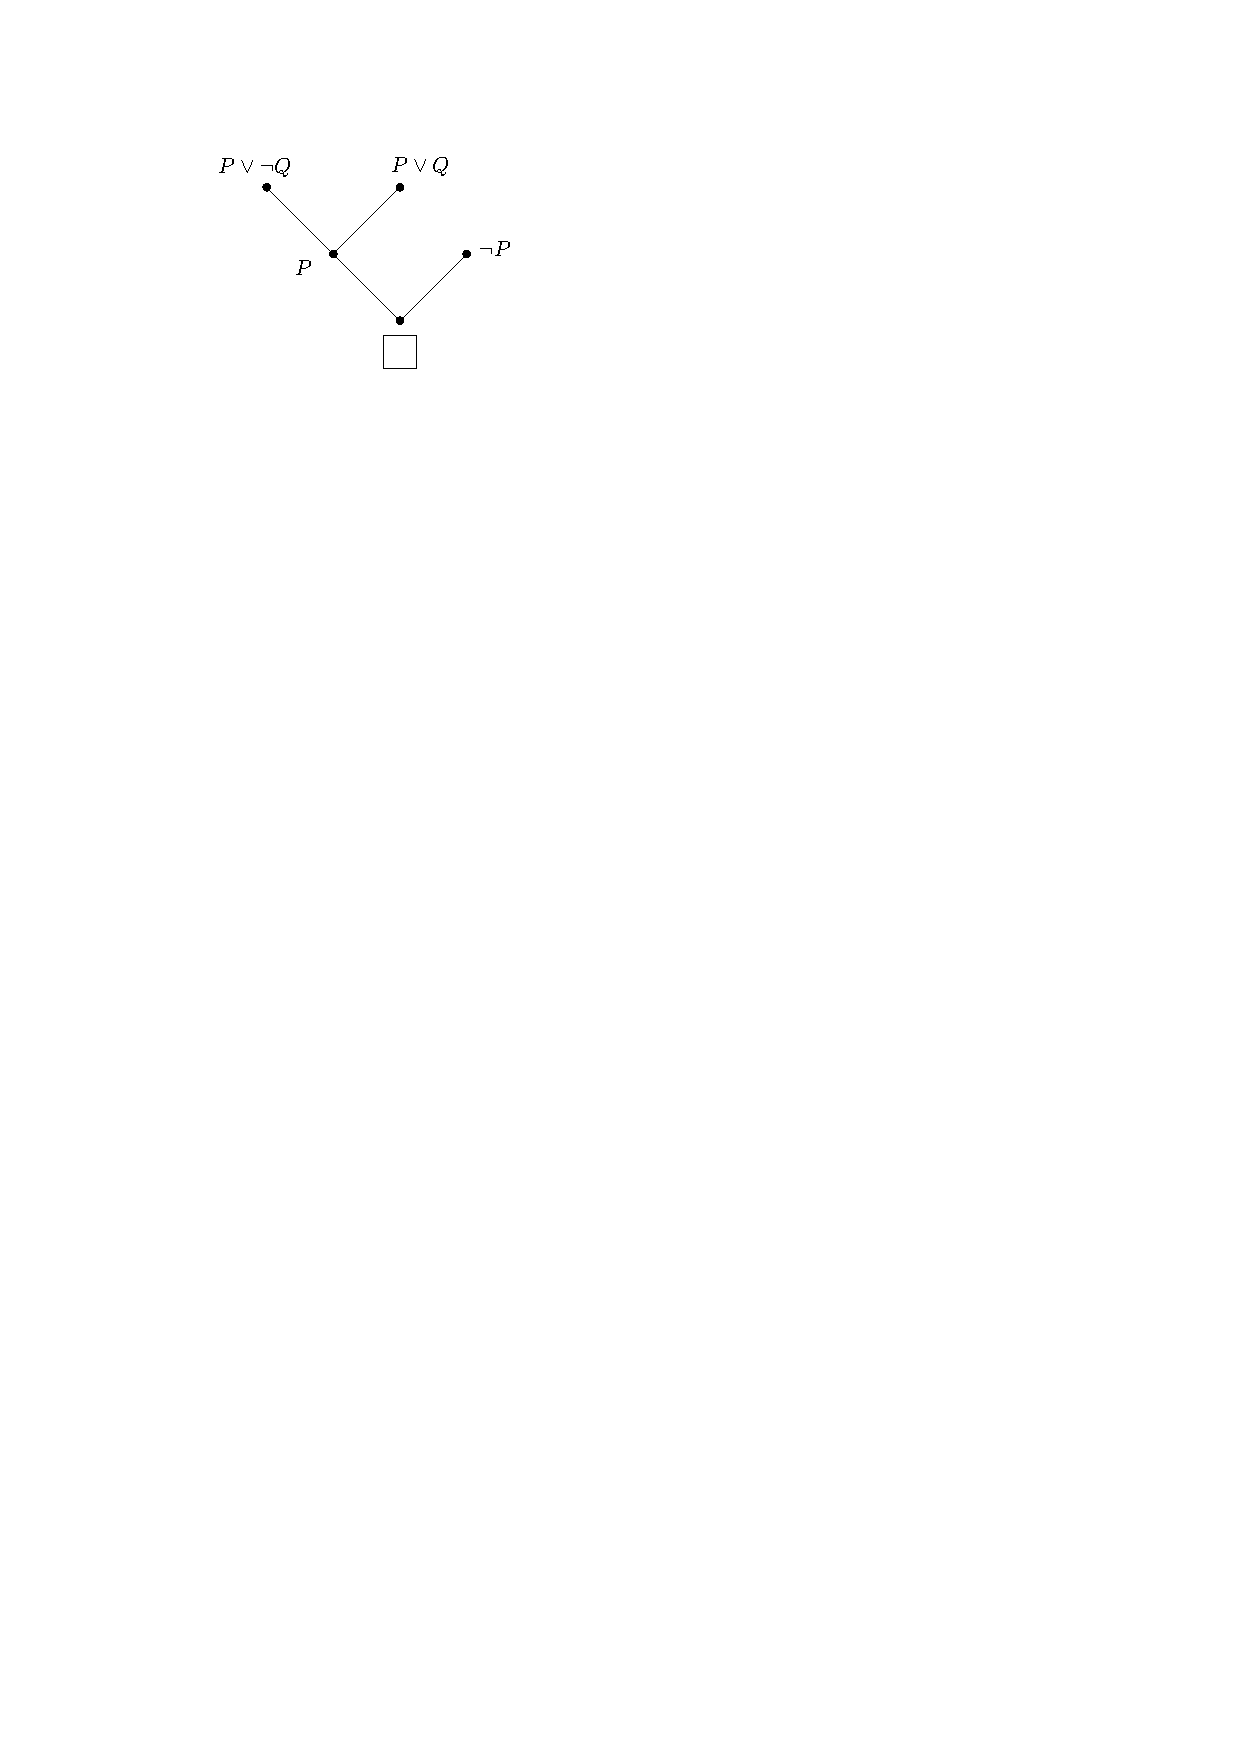
\includegraphics{image/归结-3.pdf}
        \end{figure}
    \end{enumerate}
\end{example}
\begin{definition}[空子句]
    不含任何文字的子句称为空子句。
    
    由于空子句不含有任何文字,也就不能被任何解释所满足因此空子句是永假的,不可满足的。
\end{definition}
\begin{note}
    归结中需要注意的问题2
    \begin{itemize}
        \item \textcolor{main1}{归结结果为空子句}意味着推导出的结果为\textcolor{main1}{永假式},说明前面给出的推导条件存在着矛盾,这在用归结原理进行定理证明时会用到。
        \item 合式公式可直接归结的条件:子句内为析取,子句间为合取
        \item 合式公式归结步骤:先化为子句的合取式形式,然后对子句进行归结
    \end{itemize}
\end{note}
\begin{example}
    将$\left[ \left( R\land \lnot P \right)\lor \left( R\land Q \right) \right]\land (R\to P)$化为标准子句。
    \[
        \begin{array}{l}
            R\land \left( R\lor Q \right)\land \left( \lnot P\lor R \right)\land \left( \lnot P\lor Q \right)\land \left( \lnot R\lor P \right)\\
            =R\land \left( \lnot P\lor Q \right)\land \left( \lnot R\lor P \right)
        \end{array}
    \]
    化为标准子句后,可以进行归结
    \begin{figure}[htbp]
        \centering
        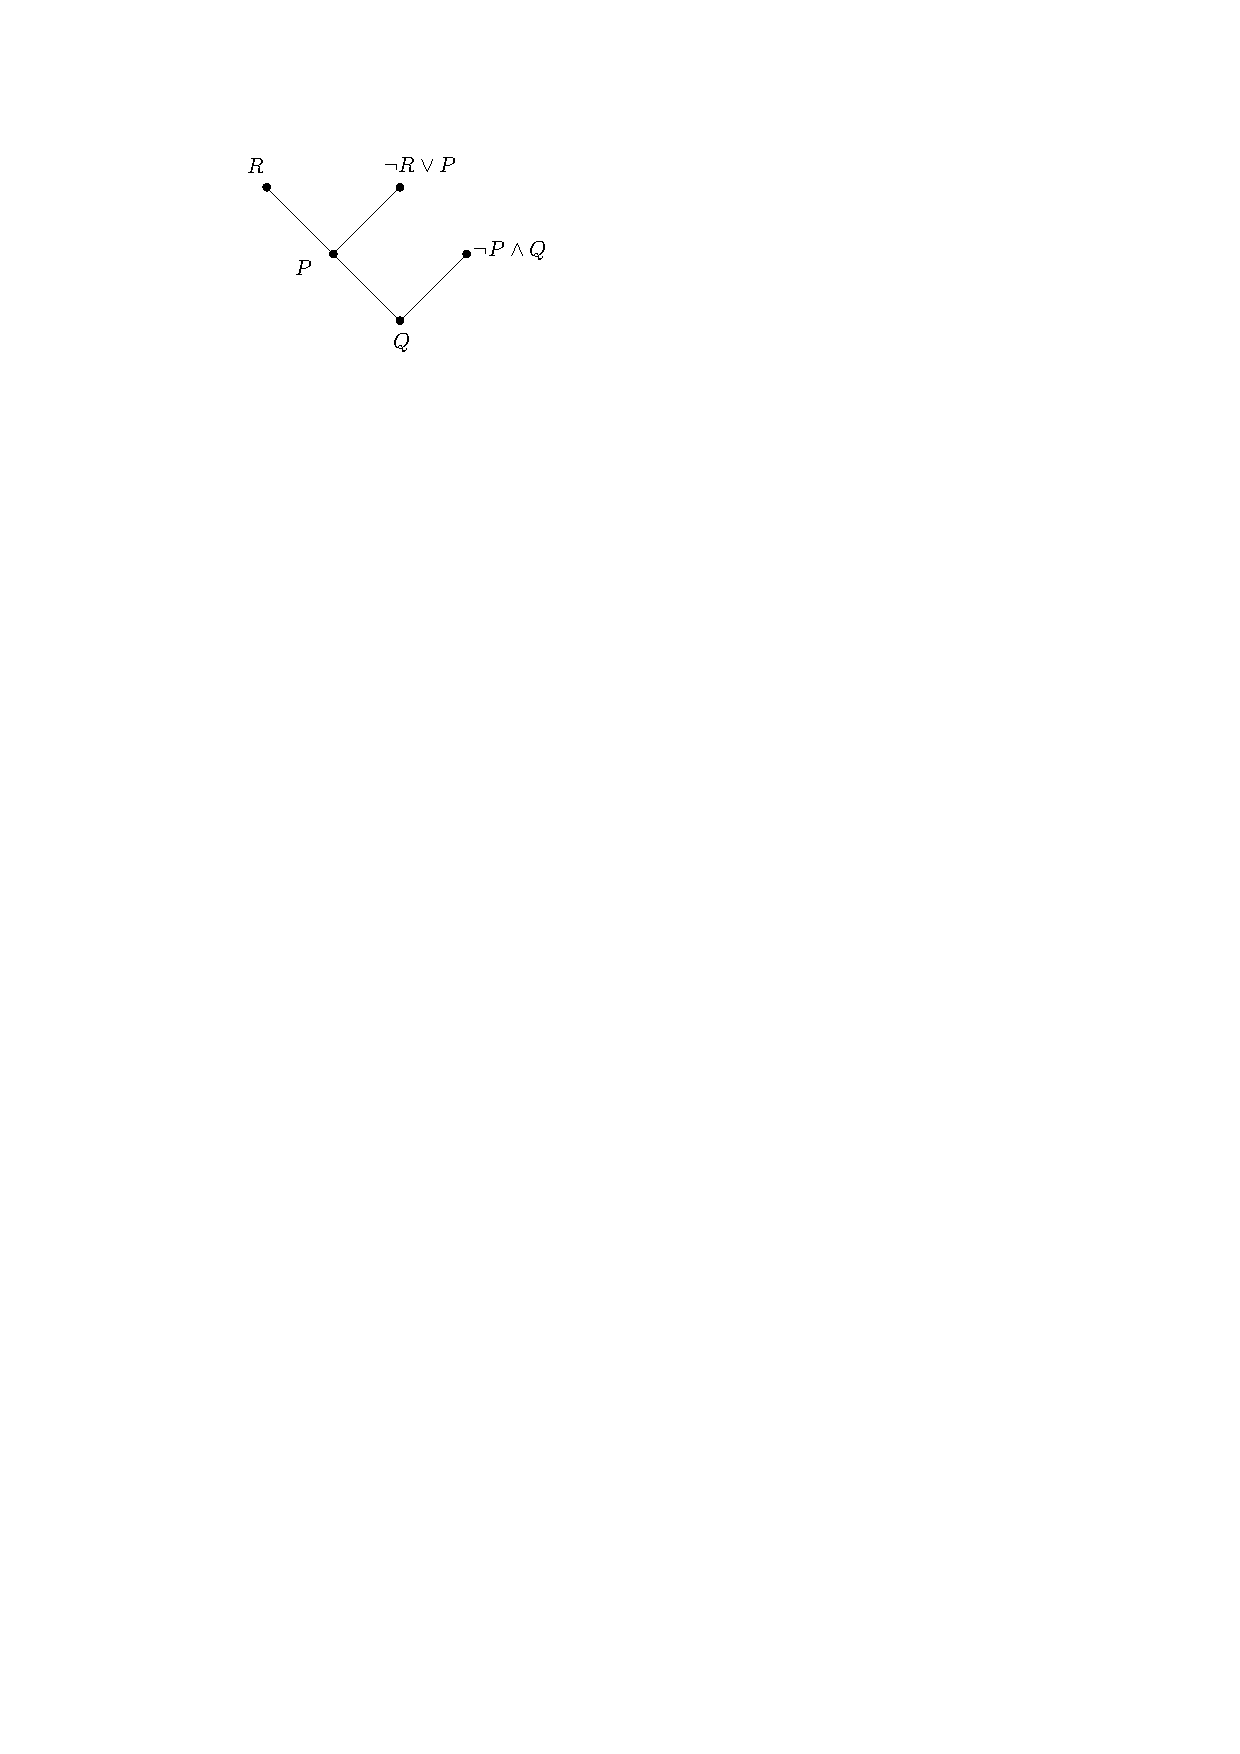
\includegraphics{image/标准-归结.pdf}
    \end{figure}
\end{example}

\begin{note}
    定理可拆分为包含条件和结论的蕴含式。
    \begin{itemize}
        \item \textcolor{main1}{如果满足“条件1”,“条件2”,$\dots$,“”,那么有“结论”}
        \item \textcolor{main1}{“条件1式”$\land$“条件2式”$\land\dots\land\dots\to$“结论式”}
    \end{itemize}
    定理证明就是要证明这个蕴含式是“永真式”
\end{note}
\begin{theorem}[基于归结的定理证明]
    证明以下:
    \begin{itemize}
        \item \textcolor{main1}{证明该式永真}:条件1式$\land$条件2式$\to$结论式
        \item \textcolor{main1}{证明该式永假}:$\lnot$(条件1式$\land$条件2式$\to$结论式)
        \item \textcolor{main1}{证明该式永假}:条件1式$\land$条件2式$\land\lnot$结论式
    \end{itemize}
\end{theorem}
\begin{note}
    归结为空意味着归结的子句间存在矛盾,推导出了永假的结果。即要证明这个式子永假,只要把这个式子归结出空就可以了。
\end{note}
\begin{example}
    机器人搬箱子,求证箱子超重。
    \begin{itemize}
        \item 机器人不能直接感知箱子是否超重
        \item 如果机器人电池有电并且箱子不超重,则机器人能够移动该箱子
        \item 已知电池有电且箱子搬不动
    \end{itemize}
    \begin{proof}
        有如下:
        设$A$:电池好、$B$:箱子超重、$C$:移动
        \begin{itemize}
            \item \textcolor{main1}{事实:}$A,\, \lnot C$
            \item \textcolor{main1}{定理:}$A\land \lnot B\to C$
            \item \textcolor{main1}{待证结论:}$B$
        \end{itemize}
        把\textcolor{main1}{所有条件和结论的非}写成合式公式,转化成标准子句:
        \[
            \begin{array}{l}
                A\land \lnot C\left( A\land \lnot B\to C \right)\land \lnot B\\
                =A\land \lnot C\left( \lnot A\lor B\lor C \right)\land \lnot B
            \end{array}
        \]        
        \begin{figure}[H]
            \centering
            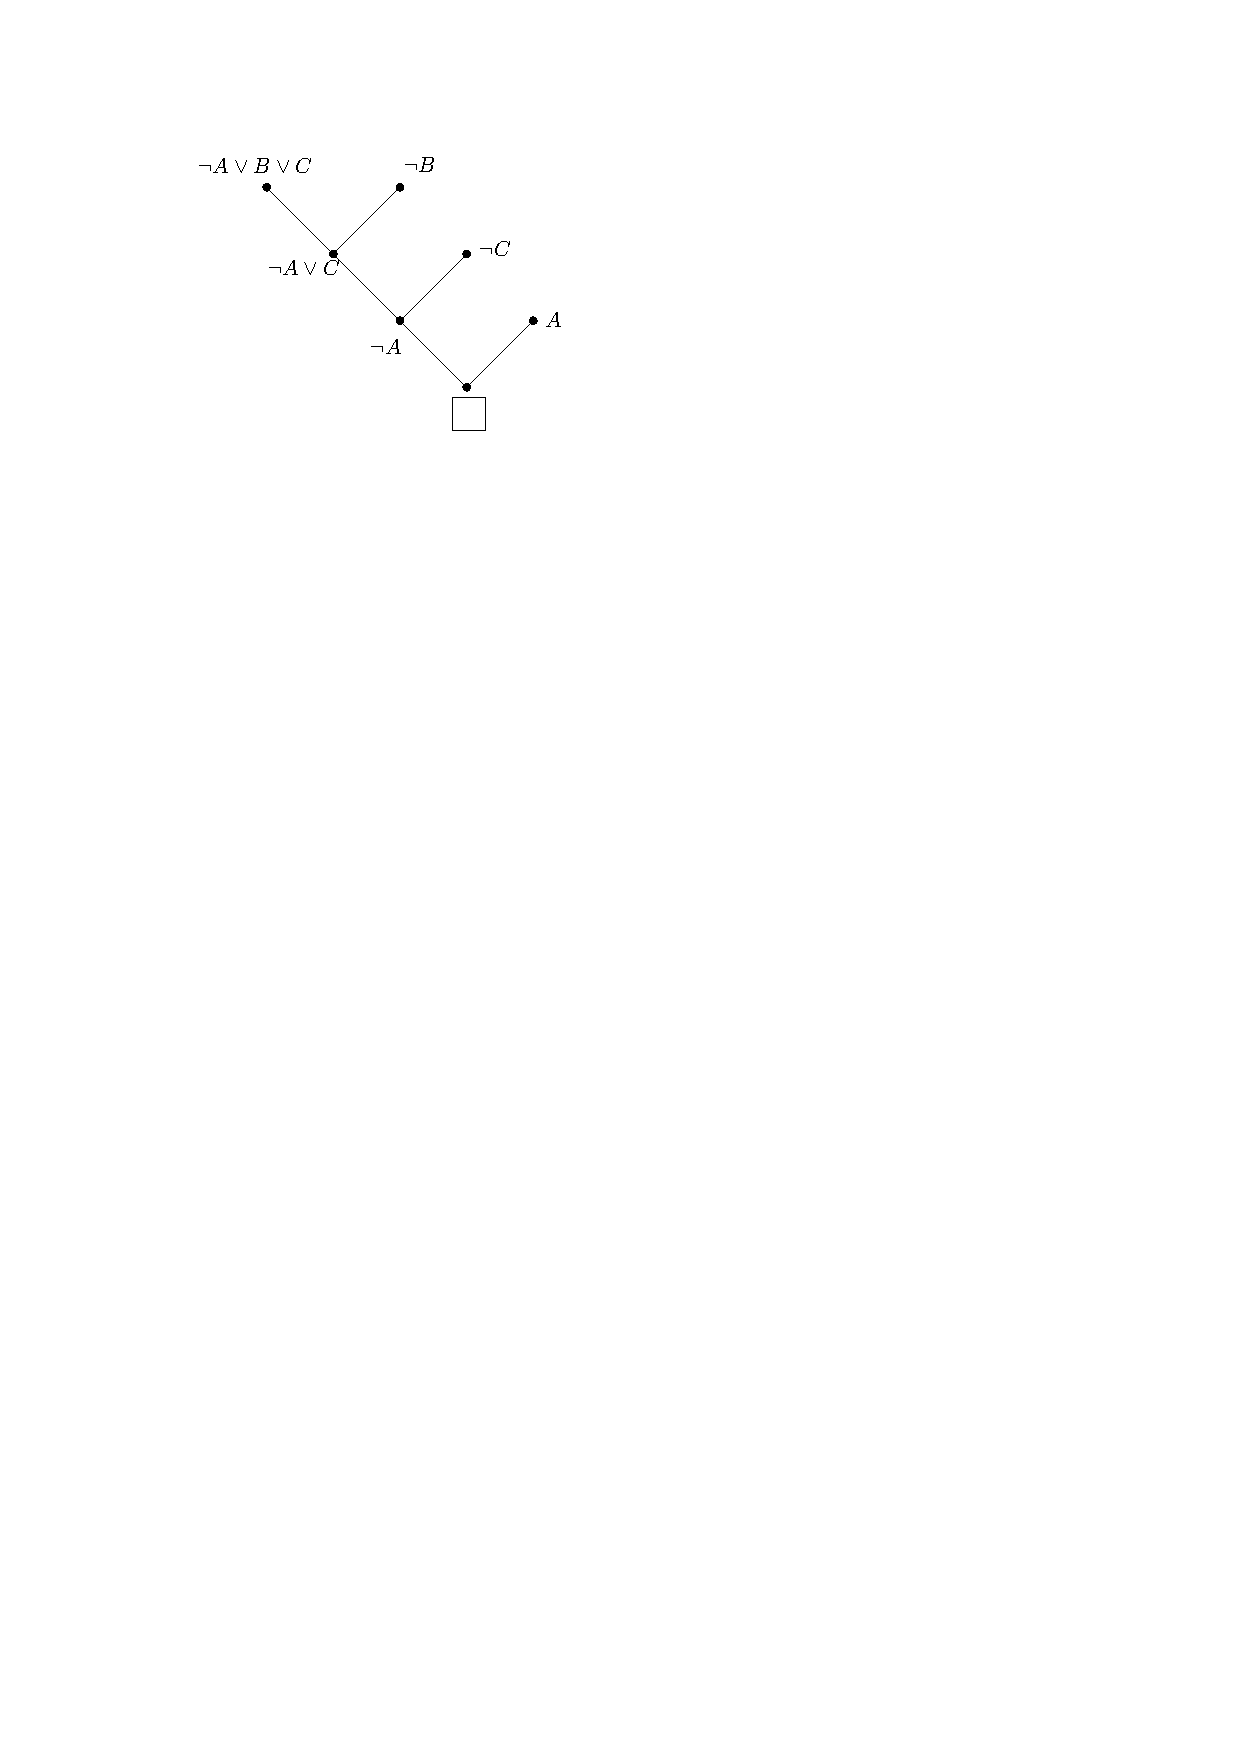
\includegraphics[width = .35\textwidth]{image/机器人搬箱子.pdf}
        \end{figure}
        证毕!
    \end{proof}
\end{example}
\begin{example}
    超级大间谍,谁是间谍?

    某个机密文件被泄露,保密局派出5个侦查员去调查
    \begin{itemize}
        \item 侦察员1说:“A与B中至少有一人作案”
        \item 侦察员2说:“B与C中至少有一人作案”;
        \item 侦察员3说:“C与D中至少有一人作案”;
        \item 侦察员4说:“A与C中至少有一人与此案无关”;
        \item 侦察员5说:“B与D中至少有一人与此案无关”。
    \end{itemize}
    证明:如果5个侦察员的话都可信,那么B和C都是间谍。
    \begin{proof}
        化为字句集合:C1:$A\lor B$、C2:$B\lor C$、C3:$C\lor D$、C4:$\lnot A \lor \lnot C$、C5:$\lnot B \lor \lnot D$、T1:$\lnot B\lor \lnot C$。把\textcolor{main1}{所有条件C1-C5和结论的非T1}写成合式公式
        \begin{figure}[H]
            \centering
            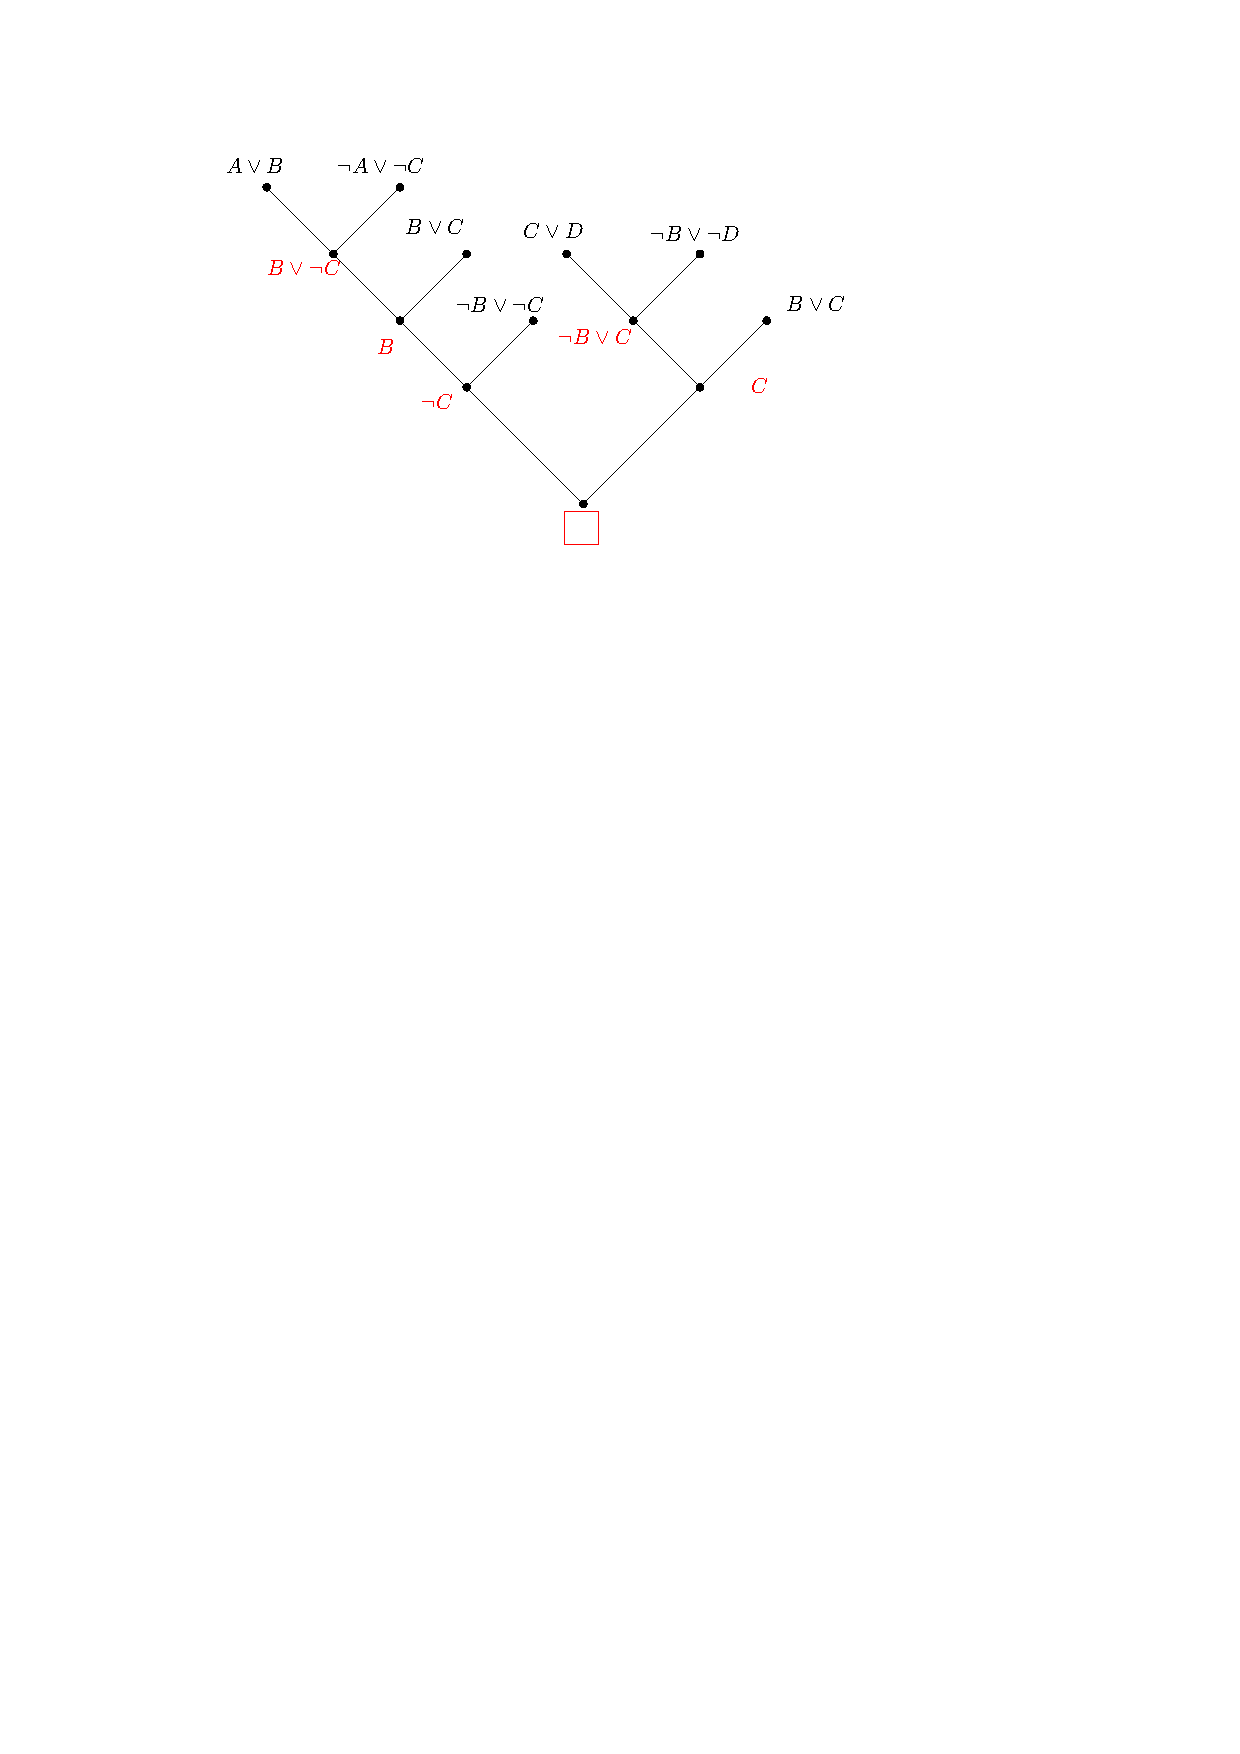
\includegraphics[width = .5\textwidth]{image/谁是间谍.pdf}
        \end{figure} 
        证毕!
    \end{proof}
\end{example}
采用归结原理进行命题逻辑定理证明的基本思想是
\begin{enumerate}[A]
    \item 归纳法
    \item 演绎法
    \item \textcolor{main1}{反证法}
    \item 枚举法
\end{enumerate}

\subsection{逻辑谓词}
\begin{note}
    命题逻辑的局限性:
    \begin{itemize}
        \item 不能表示事务的共同属性
        
        “亚里士多德是人,牛顿是人”需要用两个独立的命题来表示。这两个命题都是不可拆分的原子命题,两个命题共同的部分没法表示。
        \item 不能表达原子命题内部结构
        
        在这个原子命题中无法“张三和李四是同学”体现张三和李四的关系。
    \end{itemize}
\end{note}
\subsubsection{谓词逻辑的基本概念}
谓词逻辑由个体词、谓词、联结词及量词组成。
\begin{definition}[个体词(项)]
    指谓词描述的对象,能够独立存在的客体。

    \begin{itemize}
        \item \textcolor{main1}{常量:}张三、A、$\dots$,通常是对象的名字
        \item \textcolor{main1}{变量:}习惯上用小写字母表示,如x、 z等。Human(x)
        \item \textcolor{main1}{函数:}习惯上用小写字母或字母串表示,如$f,\,g$等。比如: father(小李)、LeftLeg (小李)、 sum(x,y)
    \end{itemize}
\end{definition}
\begin{definition}[谓词]
    用来刻画个体词的\textcolor{main1}{属性}或个体词之间的\textcolor{main1}{关系}
    
    \begin{itemize}
        \item 表示属性
        \item 表示关系
    \end{itemize}

    谓词不能单独使用,它必须与个体词结合才能构成谓词公式。
\end{definition}

\begin{definition}[联结词]
    表示谓词之间的关系
    \begin{itemize}
        \item 合取$\land$
        \item 析取$\land$
        \item 蕴含$\to$
        \item 非$\lnot$
    \end{itemize}
\end{definition}
\begin{definition}[量词]
    说明个体变量的取值范围。
    
    \begin{itemize}
        \item 全称量词,     
        表示“所有”,$\forall$
        \item 存在量词,        
        表示“存在”,$\exists$
    \end{itemize}
\end{definition}
\begin{note}
    使用量词应注意
    \begin{itemize}
        \item 一般情况下,$\to$是与$\forall$是一起的主要连接词
        \item 一般情况下,$\land$是与$\exists$是一起的主要连接词
    \end{itemize}
\end{note}
\begin{definition}[量词的辖域]
    \textcolor{main1}{量词的辖域}是邻接量词之后的最小子公式,\textcolor{main1}{因此除非辖域是个原子公式,否则应该在该子公式两端有括号}

    \begin{itemize}
        \item 例:$\forall x\, P(x)\to Q(x)$
        
        $\forall x$的辖域是$P(x)$
        \item 例:$\exists x\, (P(x)\to Q(x))\lor P(y,z)$
        
        $\exists x$的辖域是$P(x)\to Q(x)$
    \end{itemize}
\end{definition}
\begin{definition}[约束变元和自由变元]
    在一个量词的辖域中与该量词的\textcolor{main1}{指导变元}相同的变元称为\textcolor{main1}{约束变元},其他变元称为自由变元。

    例如:$\forall \textcolor{red}{x}\left( P(\textcolor{blue}{x})\lor Q(y) \right)\land (\exists \textcolor{red}{z})\left( R(\textcolor{blue}{z}) \right)$
\end{definition}
\begin{note}
    多个量词并用时

    $\forall x\exists yP(x,y)$与$\exists y\forall xP(x,y)$不等价

    $x,\,y$分别表示一个自然数;$P(x,y):,\,y>x$

    多个全称量词和存在量词混用时,顺序不可以颠倒。
\end{note}
\subsubsection{逻辑谓词的归结}
\begin{note}
    置换注意事项:

    \begin{itemize}
        \item 只有变量才能被置换,常量和函数不能被置换。
        \item 置换要整体进行,即不同位置的同一变量要一起置换。
        \item \textcolor{main1}{置换的变量不能出现在置换项中。} 即:对于置换$s = \left\{ t_1/x_1,t_2/x_2,\cdots,t_n/x_n \right\}$,任一变量$x_i$,不能出现在某个置换项$t_i$,中。
        \item 同一个变量不能被多个置换项同时置换。
        \item 置换不符合交换律:$s_1s_2\neq s_2s_1$
    \end{itemize}
\end{note}
\begin{note}
    置换与合一
    \begin{itemize}
        \item \textcolor{main1}{原始知识:}
        
        所有人都会死

        亚里士多德是人
        \item \textcolor{main1}{谓词公式:}
        
        \[
            \begin{array}{l}
                \forall x\,\left( Human(x)\to WillDie(x) \right)\\
                Human(Aristotle)
            \end{array}
        \]

        \item  \textcolor{main1}{化成子句:}
        
        \[
            \begin{array}{l}
                \lnot Human(x)\lor WillDie(x)\\
                Human(Aristotle)
            \end{array}
        \]
        这两个子句不能归结,因为形式上并不完全相同
        \item 用亚里士多德替换$x$,可以进行归结
        \item \textcolor{main1}{合一:}寻找项对变量的置换,以使两个合式公式表达一致。若存在一个置换$s$使得表达式集合$\{E_i\}$中每个元素经置换后有:$E_1s =E_2s = E_3s = \dots,$则称表达式集$\{E_i\}$是可合一的,这个置换$s$称为合一元。
        \item \textcolor{main1}{最一般合一元}$\sigma$(The most general unifier,mgu),$\left\{ w_i \right\}$的$\sigma$有如下特性

        如果$\theta$是$\left\{ w_i \right\}$任意合一元,那么存在一个置换$\lambda$使得$\left\{ w_i \right\}\theta = \left\{ w_i \right\}\sigma\lambda$,即$\sigma$是能够使合一的最小置换。
        \item 为何最需要最一般合一元
        
        求证:$\left\{ \lnot P(x,y)\lor \lnot Q(y,z), P(A,w) \right\}\Rightarrow \lnot Q(B,C)$
        \begin{figure}[htbp]
            \centering
            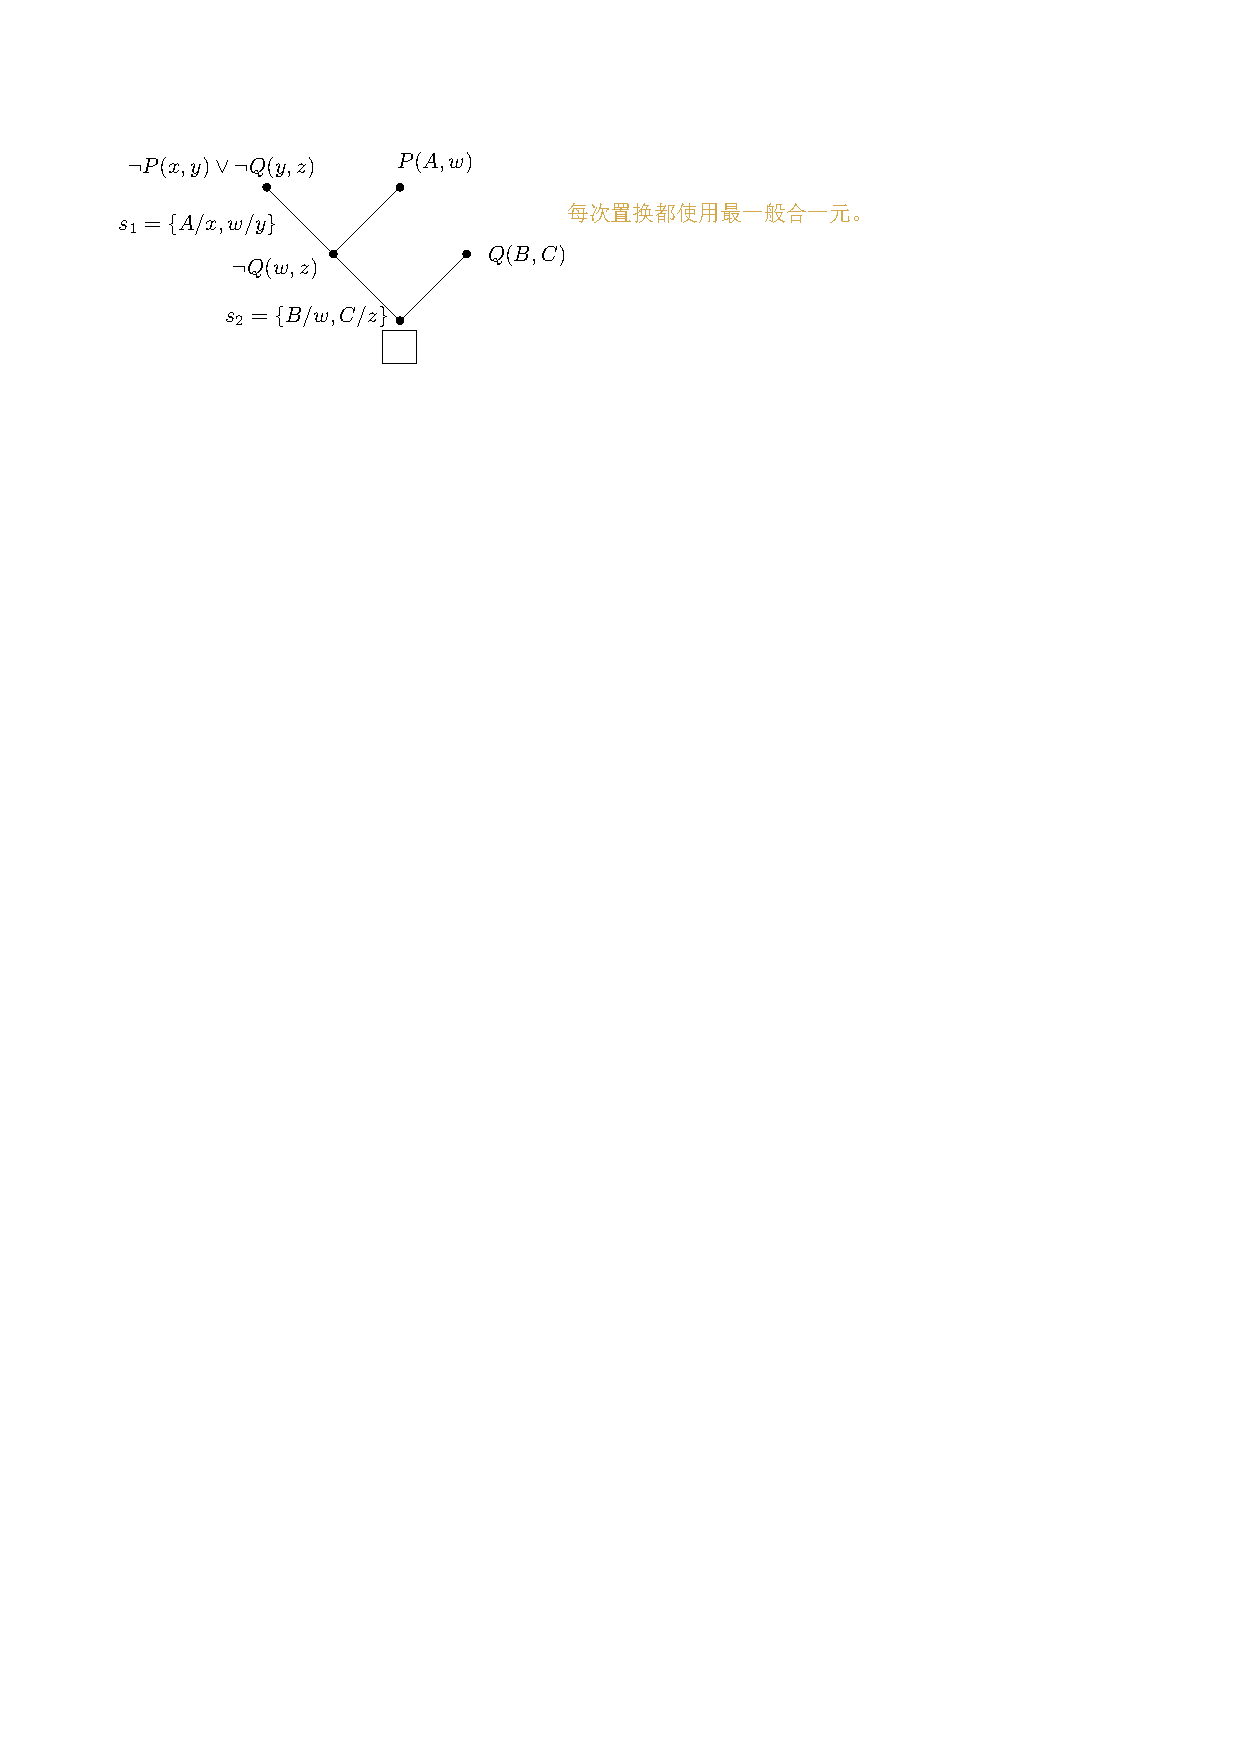
\includegraphics{image/最一般合一元.pdf}
        \end{figure}        
    \end{itemize}    
\end{note}
\begin{theorem}[归结原理]
    定理的证明过程:
    \begin{enumerate}
        \item 将\textcolor{main1}{结论的非}与\textcolor{main1}{所有条件式}进行合取,得到待证明的合式公式;
        \item 将上述合式公式化成可以归结的子句集形式;(\textcolor{main1}{子句间为合取关系,子句内为析取形式})
        \item 对上述式子进行归结,如果\textcolor{main1}{归结为空,则定理得证。}
    \end{enumerate}
\end{theorem}
\begin{note}
    命题演算中公式标准化过程:
    \begin{itemize}
        \item 消除蕴含符号
        
        使用蕴含表达式$P\to Q\equiv \lnot P\land Q$
        \item 否定深入
        
        减少否定符号的范围,否定符号$\lnot$最多只用到一个命题符号上
        \item 转换成子句的合区范式
        
        字句内析取、子句间合区
        \item 形成子句合集
    \end{itemize}
\end{note}
\begin{note}
    谓词公式化为标准子句:

    目的:将谓词公式化为\textcolor{main1}{机器可以接收、处理}的标准形式,这种标准形式是\textcolor{main1}{不含量词的子句集}
    相比命题公式标准化的难点:
    \begin{itemize}
        \item 全称量词和存在量词处理
        \item 各种变量名称如何处理
    \end{itemize}

    \textcolor{main1}{标准化步骤}:
    \begin{enumerate}
        \item 消去蕴含符号
        \item 否定深入(减少否定符号的范围)
        \item \textcolor{main1}{变量标准化(每个量词有唯一的变量符号)}
        
        \textcolor{main1}{例如:}
        \begin{itemize}
            \item 量词辖域不重叠
            
            $\left( \forall x \right)P(x)\lor \left( \forall x \right)Q(x)$转化为$\left( \forall x \right)P(x)\lor \left( \forall \textcolor{main1}{y} \right)Q(\textcolor{main1}{y})$
            \item 量词辖域重叠
            
            $\left( \forall x \right)\left( P(x)\to \left( \exists x \right)Q(x) \right)$转化为$\left( \forall x \right)\left( P(x)\to \left( \exists \textcolor{main1}{y} \right)Q(\textcolor{main1}{y}) \right)$
        \end{itemize}
        通过改变变量名称,使每个量词修饰的变量有自己唯一的变量名。(\textcolor{main1}{不同量词修饰的变量符号不同})
        \item \textcolor{main1}{消去存在量词}
        
        \begin{itemize}
            \item 如果存在量词不受全称量词修饰:直接例化即可
            
            $\exists xP(x)$实例化为$P(A)$,要求$A$必须是新的常量符号
            \item 如果存在量词受全称量词修饰:使用Skolem函数
            
            $\left( \forall x \right)\left( \left( \exists y \right)\operatorname{Cap}(x,y) \right)$,用$g(x)$替换$y$,消去存在量词得到$\left( \forall x \right)\operatorname{Cap}(x,g(x))$,Skolem函数必须是新的
        \end{itemize}

        消去存在量词,\textcolor{main1}{存在量词}的\textcolor{main1}{约束变元}使用关于\textcolor{main1}{全称量词}的\textcolor{main1}{指导变元的函数}来代替

        如果存在量词处在多个全称量词的辖域内,则同时受多个全称量词共同影响,Skolem函数为关于多个全称量词修饰变量的函数。
        \item \textcolor{main1}{消去全称量词}
        \begin{itemize}
            \item 直接将全称量词的符号去除。
            \item 经过前面几步,已经不存在量词修饰的变量,剩下的变量可以任意取值,所以没必要保留全称量词符号。
        \end{itemize}

        \item 把公式化为合取范式(子句间为合取关系,子句内为析取形式)写成子句形式(消除合取符号)
        \item \textcolor{main1}{更换变量名称(一个变量符号不用于多个子句)}
        
        更换变量符号的名称,使一个变量符号不出现在一个以上的子句中。

        对于子句集
        \[
            \begin{array}{l}
                \{ \lnot P(x_1)\lor \lnot P(y)\lor P(f(x_1,y)),\\
                    \lnot P(x_2)\lor Q(x_2,g(x_2))\\
                    \lnot P(x_3)\lor \lnot P(g(x_3))\}
            \end{array}
        \]
    \end{enumerate}
\end{note}
\begin{example}
    将下列谓词公式化为标准子式
    \begin{itemize}
        \item $\forall x\left( \left( \forall y P(x,y) \right) \to \lnot \left( \forall y\left( Q(x,y)\to R(x,y) \right) \right) \right)$
        \begin{enumerate}
            \item 消去蕴含符号
            \[
                \forall x\left(\lnot \left( \forall y P(x,y) \right) \lor \lnot \left( \forall y\left( \lnot Q(x,y)\lor R(x,y) \right) \right) \right)
            \]
            \item 否定深入
            \[
                \forall x\left(\exists y \lnot P(x,y)  \lor \left( \exists y\left( Q(x,y)\land \lnot R(x,y) \right) \right) \right)            
            \]
            \item 变量标准化
            \[
                \forall x\left(\exists y \lnot P(x,y)  \lor \left( \exists z\left( Q(x,z)\land \lnot R(x,z) \right) \right) \right)
            \]
            \item 消去存在量词
            \[
                \forall x\left(\lnot P(x,f(x))  \lor \left( Q(x,g(x))\land \lnot R(x,g(x)) \right) \right)
            \]
            \item 消去全称量词
            \[
                \lnot P(x,f(x))  \lor \left( Q(x,g(x))\land \lnot R(x,g(x)) \right)
            \]
            \item 化为合取范式 
            \[
                \left( \lnot P(x,f(x)) \lor Q(x,g(x)) \right) \land  \left(\lnot P(x,f(x)) \lnot R(x,g(x)) \right)
            \]
            \item 化为子句集形式
            \[
                \begin{array}{l}
                    \{  \lnot P(x,f(x)) \lor Q(x,g(x)),\\ 
                    \lnot P(x,f(x)) \lnot R(x,g(x)) \}
                \end{array}
            \]
            \item 更换变量名称
            \[
                \begin{array}{l}
                    \{  \lnot P(x,f(x)) \lor Q(x,g(x)),\\ 
                    \lnot P(y,f(y)) \lnot R(y,g(y)) \}
                \end{array}
            \]
        \end{enumerate}
        \item $\left( (\exists x)P(x)\lor (\exists x)Q(x) \right)\to \left( (\exists x)(P(x)\lor Q(x)) \right)$
        \begin{enumerate}
            \item 消去蕴含符号
            \[
                \lnot \left( (\exists x)P(x)\lor (\exists x)Q(x) \right)\lor \left( (\exists x)(P(x)\lor Q(x)) \right)
            \]
            \item 否定深入
            \[
                \left((\forall x)\lnot P(x)\land (\forall  x)\lnot Q(x) \right)\lor \left( (\exists x)(P(x)\lor Q(x)) \right) 
            \]
            \item 变量标准化
            \[
                \left((\forall x)\lnot P(x)\land (\forall  y)\lnot Q(y) \right)\lor \left( (\exists z)(P(z)\lor Q(z)) \right) 
            \]
            \item 消去存在量词
            \[
                \left((\forall x)\lnot P(x)\land (\forall  y)\lnot Q(y) \right)\lor \left( P(A)\lor Q(A)\right) 
            \]
            \item 消去全称量词
            \[
                \left(\lnot P(x)\land \lnot Q(y) \right)\lor \left( P(A)\lor Q(A)\right) 
            \]
            \item 化为合取范式
            \[
                \left(\lnot P(x)\lor P(A)\lor Q(A) \right)\land \left(\lnot Q(y)\lor P(A)\lor Q(A) \right)
            \]
            \item 化为子句集形式
            \[
                \begin{array}{l}
                    \{  \lnot P(x)\lor P(A)\lor Q(A),\\ 
                    \lnot Q(y)\lor P(A)\lor Q(A) \}
                \end{array}
            \]
            \item 更换变量名称
            \[
                \begin{array}{l}
                    \{  \lnot P(x)\lor P(A)\lor Q(A),\\ 
                    \lnot Q(y)\lor P(A)\lor Q(A) \}
                \end{array}
            \]
        \end{enumerate}
    \end{itemize}
\end{example}
\subsubsection{定理证明和求解}
\begin{note}
    谓词定理自动归结证明过程
    \begin{itemize}
        \item 将合式公式化为子句集的过程不同
        
        因为谓词逻辑引入了个体词和量词,所以化为子句时和命题化为子句的步骤是不一样的
        \item 归结过程不同
        
        因为个体词有变量和常量,所以谓词归结的过程和命题归结相比需要置换和合一。
    \end{itemize}
\end{note}
\begin{example}
    机器人搬箱子的归结证明

    已知:27号房间的所有箱子都比29号房间的箱子小。现在机器人知道箱子A在27号或29号房间中,箱子B在27号房间中,且B不比A小。\textcolor{main1}{试证明箱子A在27号房间中}
    \begin{proof}
        有以下谓词公式
        \begin{itemize}
            \item F1:\,$ \forall x\forall y\left( P(x)\land P(y)\land Inroom(x,27)\land Inroom(y,29)\to Smaller(x,y)  \right) $
            \item F2:\,$ Inroom(A,27)\lor Inroom(A,29) $
            \item F3:\,$ Inroom(B,27)\land \lnot Smaller(B,A) $
            \item F4:\,$P(A)$
            \item F5:\,$P(B)$
            \item T:\,$ \lnot Inroom(A,27) $
        \end{itemize}    
        化为子句集形式
        \begin{itemize}
            \item C1:\,$ \lnot P(x)\lor \lnot P(y)\lor \lnot Inroom(x,27)\lor\lnot Inroom(y,29)\lor Smaller(x,y)  $
            \item C2\,:$ Inroom(A,27)\lor Inroom(A,29) $
            \item C3\,:$ Inroom(B,27) $
            \item C4\,:$ \lnot Smaller(B,A) $
            \item C5\,:$P(A)$
            \item C6\,:$P(B)$
            \item C7\,:$ \lnot Inroom(A,27) $
        \end{itemize}
        \textcolor{main1}{归结定理证明}
        \begin{figure}[htbp]
            \centering
            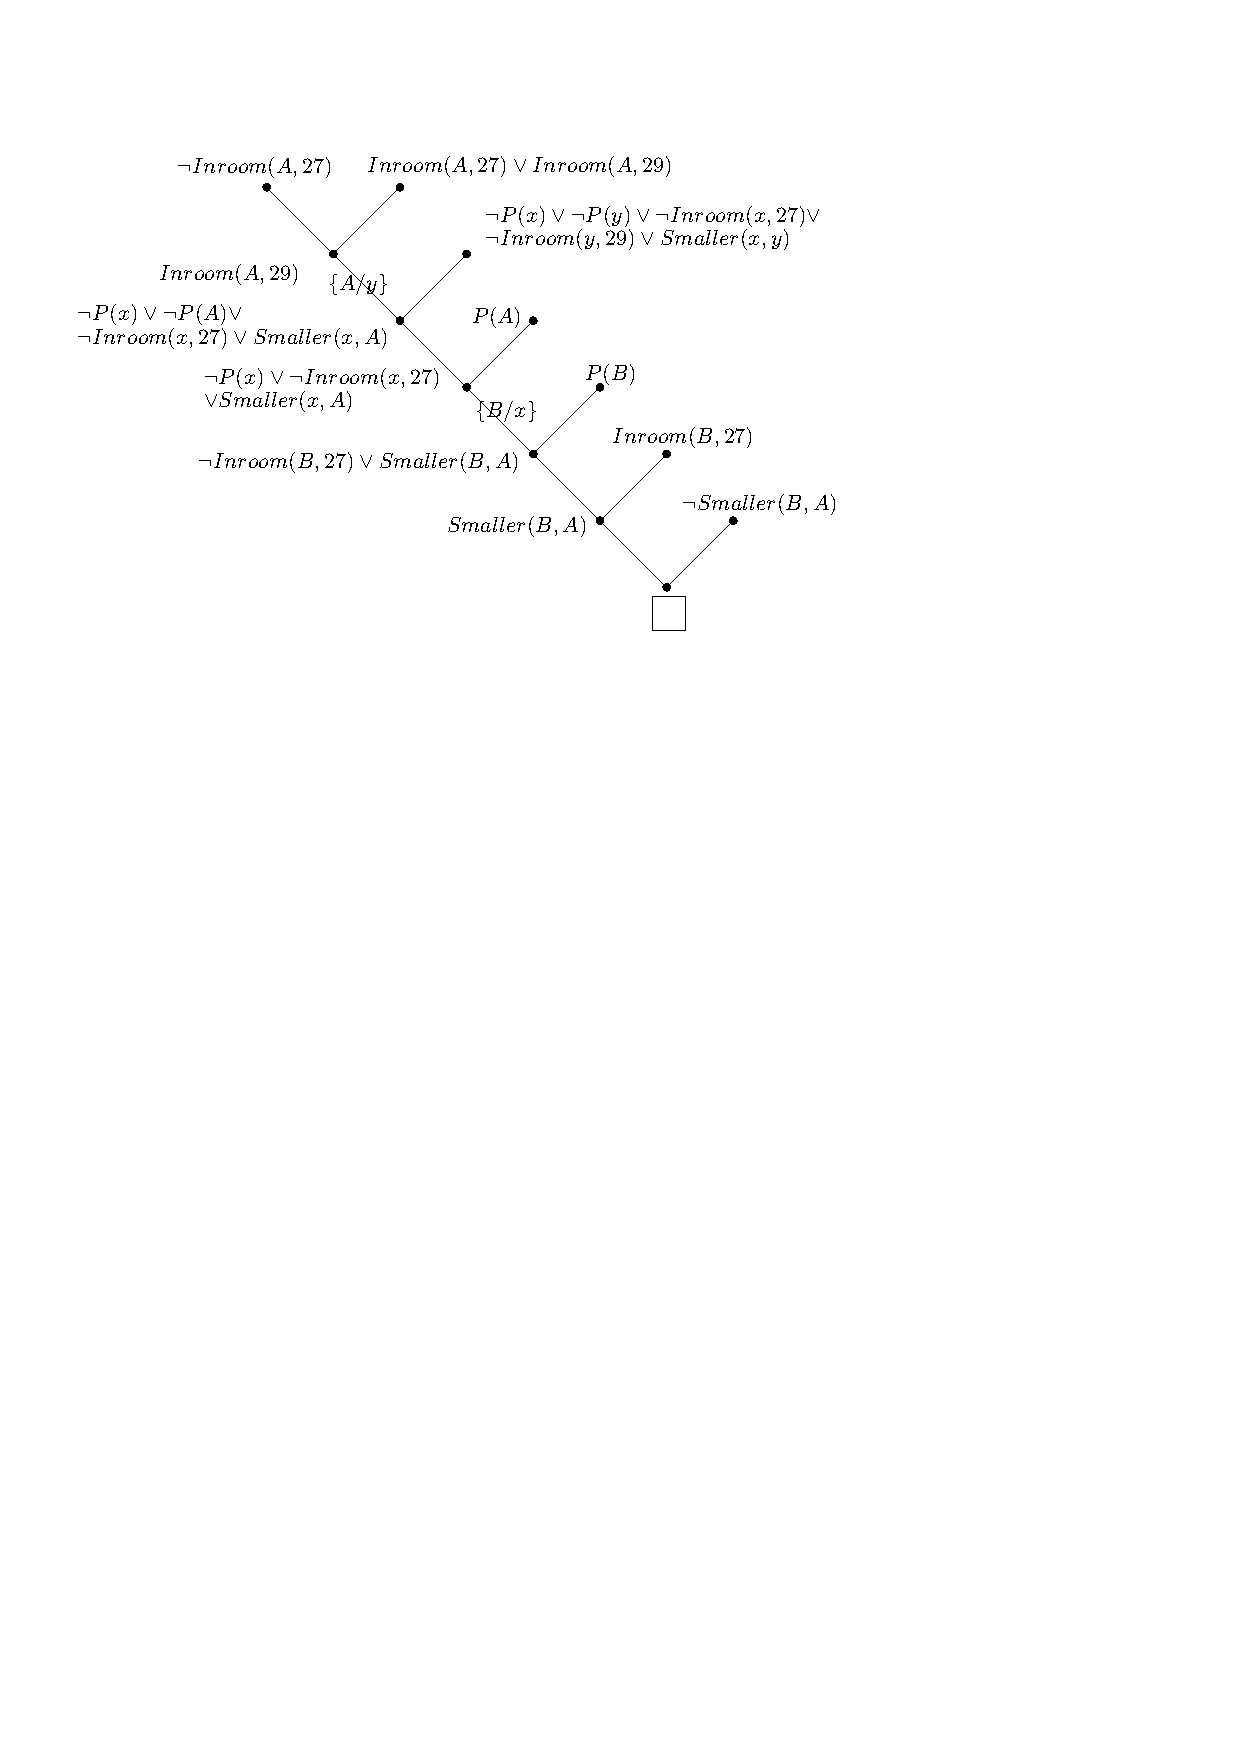
\includegraphics{image/定理证明例子.pdf}
        \end{figure}
    \end{proof}
\end{example}

\begin{example}
    机器人搬箱子的问题求解

    已知:27号房间的所有箱子都比29号房间的箱子小。现在机器人知道箱子A在27号或29号房间中,箱子B在27号房间中,且B不比A小。\textcolor{main1}{问箱子A在哪个房间?}

    \textcolor{main1}{解:}有以下谓词公式
    \begin{itemize}
        \item F1:\,$ \forall x\forall y\left( P(x)\land P(y)\land Inroom(x,27)\land Inroom(y,27)\to Smaller(x,y)  \right) $
        \item F2:\,$ Inroom(A,27)\lor Inroom(A,29) $
        \item F3:\,$ Inroom(B,27)\land \lnot Smaller(B,A) $
        \item F4:\,$P(A)$
        \item F5:\,$P(B)$
        \item T:\,$ \left( \exists u \right)\,Inroom(A,u) $
    \end{itemize}    
    化为子句集形式
    \begin{itemize}
        \item C1:\,$ \lnot P(x)\lor \lnot P(y)\lor \lnot Inroom(x,27)\lor\lnot Inroom(y,27)\lor Smaller(x,y)  $
        \item C2\,:$ Inroom(A,27)\lor Inroom(A,29) $
        \item C3\,:$ Inroom(B,27) $
        \item C4\,:$ \lnot Smaller(B,A) $
        \item C5\,:$P(A)$
        \item C6\,:$P(B)$
        \item C7\,:$ \lnot Inroom(A,u) $
    \end{itemize}
    \begin{figure}[htbp]
        \centering
        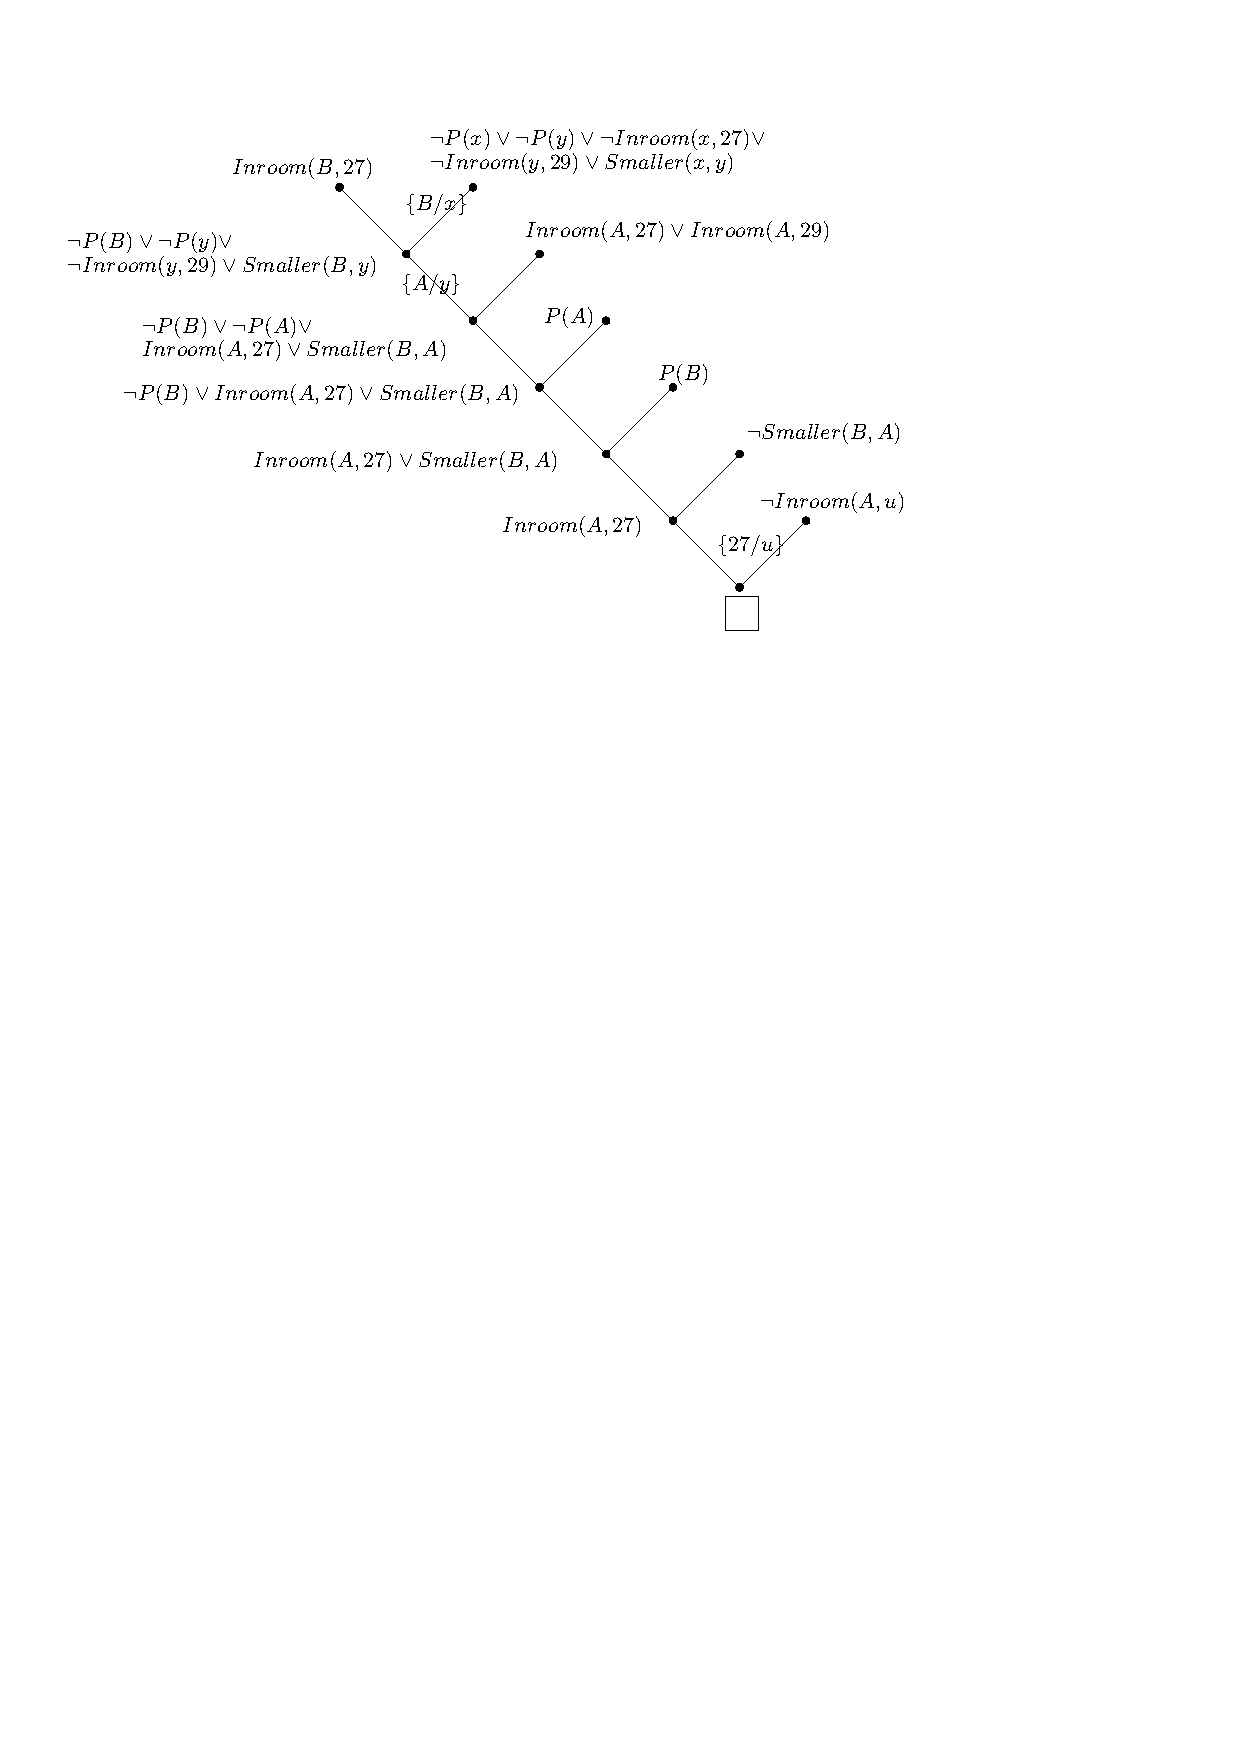
\includegraphics[width = .7\textwidth]{image/问题求解例子.pdf}
    \end{figure}

    用归结来回答由合式公式表示的关于领域知识的问题,而不只是证明一个定理。例如,不仅要证明形如$(\exists u)W(u)$的定理,而且想得到已经证明存在的$u$。
    为此,将文字$Ans(u)$加到要证明定理的否定子句中,执行归结直到只剩下一个回答文字。\textcolor{main1}{加入子句$\lnot W(u)\lor Ans(u)$}
    \begin{figure}[htbp]
        \centering
        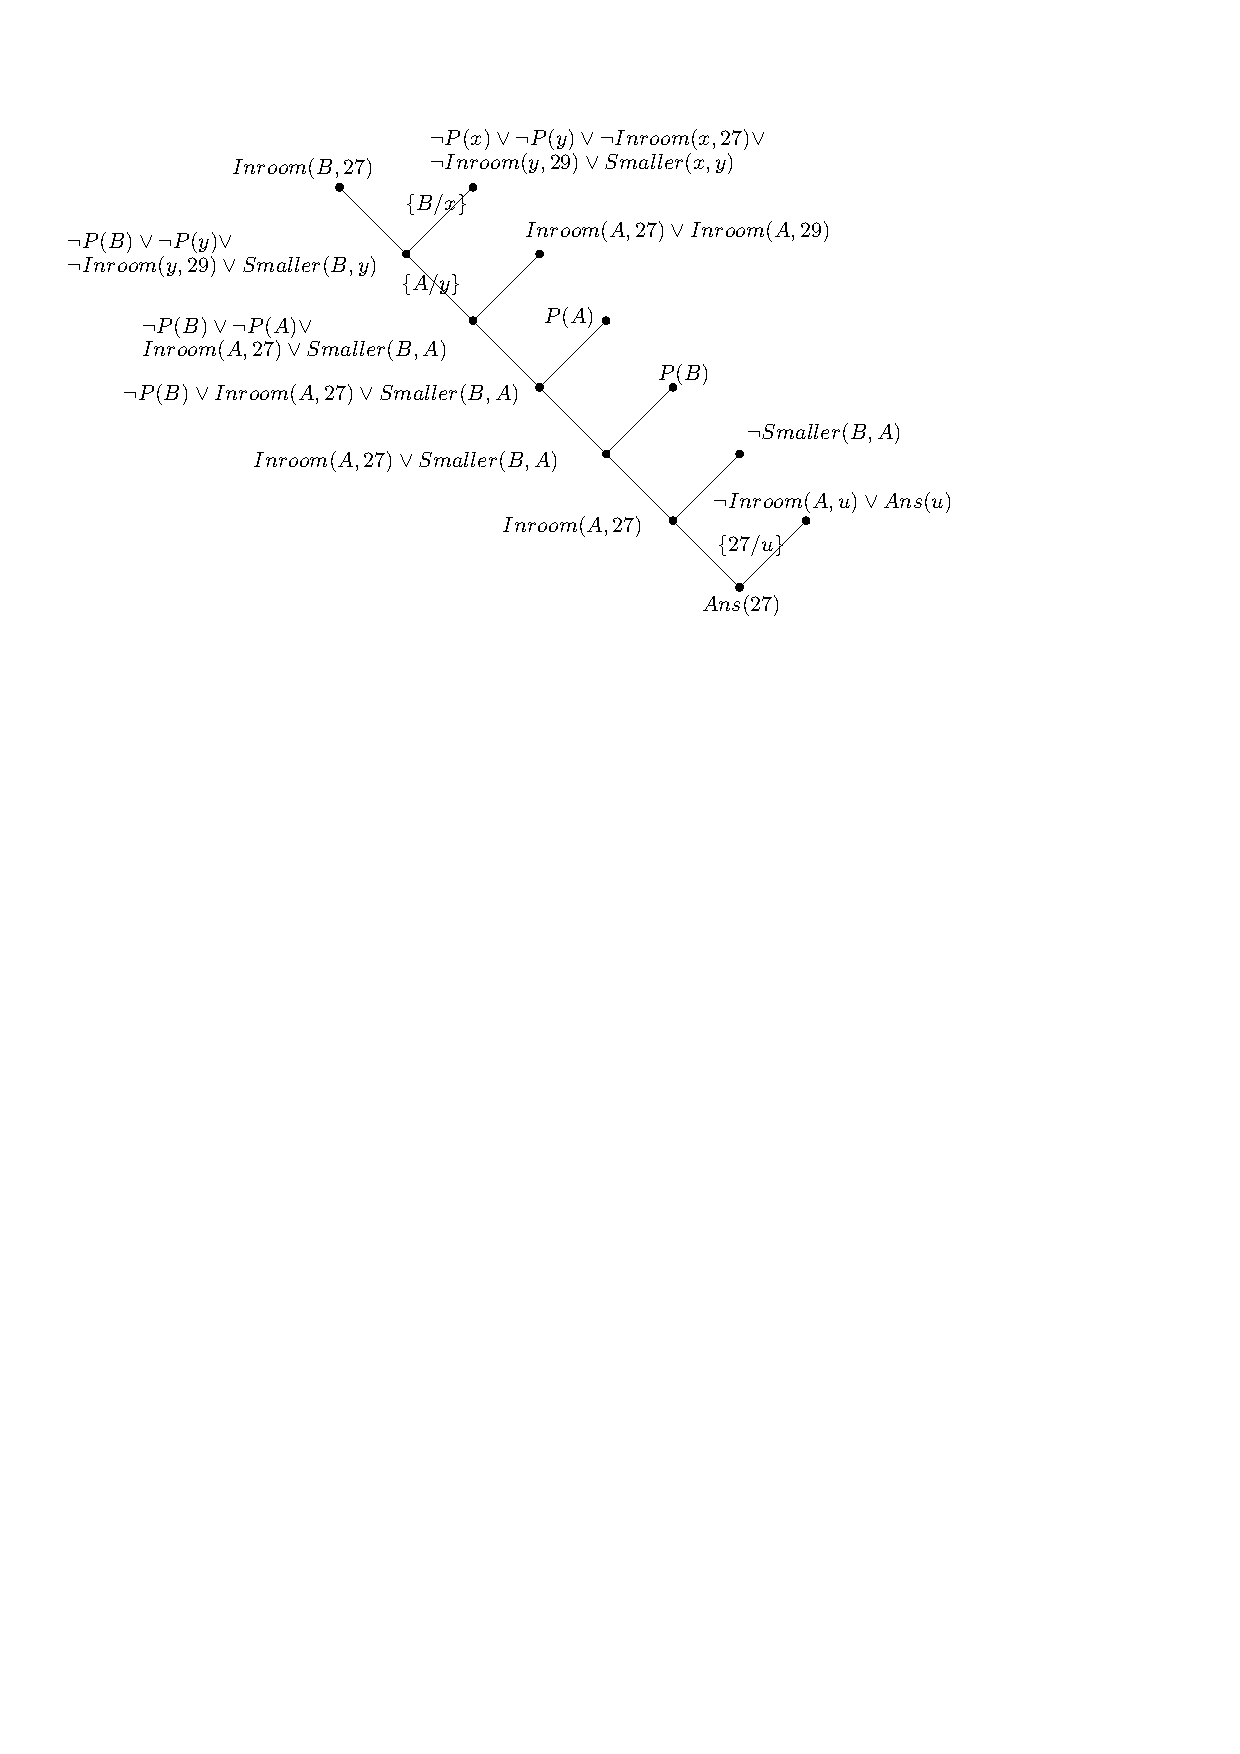
\includegraphics[width = .7\textwidth]{image/问题求解例子+Ans.pdf}
    \end{figure}
\end{example}

\subsection{不确定知识与推理}
\subsubsection{不确定性描述}
\begin{figure}[htbp]
    \centering
    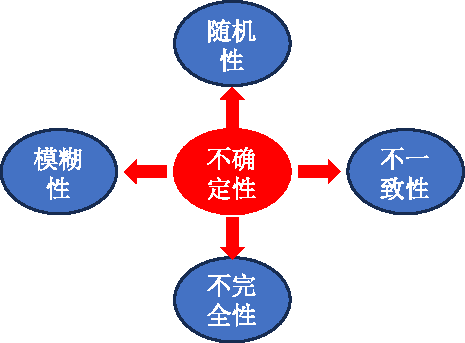
\includegraphics[scale = 0.7]{image/不确定性.pdf}
\end{figure}
\begin{itemize}
    \item 随机性
    
    如果乌云密布并且电闪雷鸣,则很可能要下暴雨。
    
    如果头痛发烧,则大概是患了感冒。
    \item 模糊性
    
    姚明是个高个子。
    
    张三和李四是好朋友。
    \item 不完全性
    
    战场上,交战双方对对手的信息掌握往往是不完全的。
    
    警方破案过程中,所掌握的关于罪犯的有关信息,往往就是不完全的。
    \item 不一致性
    
    牛顿运动定律对于宏观世界是正确的,但对于微观世界和宇观世界却是不适合的。
\end{itemize}
\subsubsection{不确定领域的知识表示}
\begin{example}
    例医疗诊断中,医生知道脑膜炎会引起病人脖子僵硬(如70\%的概率)﹔此外,医生还了解一些无条件事实:病人患脑膜炎先验概率1/50000,而任何一个病人脖子僵硬的先验概率为1\%。目前有一病人脖子僵硬,判断是否为脑膜炎。

    令$s$表示“病人脖子僵硬”,$m$表示“病人患有脑膜炎”,则有
    \[
        \begin{array}{l}
            p(s|m) = 0.7\\
            p(m) = 1/50000\\
            p(s) = 0.01\\
            p(m|s) = \dfrac{p(s|m)p(m)}{p(s)} = \dfrac{0.7\times 1/50000}{0.01} = 0.0014
        \end{array}
    \]
\end{example}
\subsubsection{贝叶斯网络}
\begin{definition}[条件概率表(CPT)]
    对于一个变量$Z$,CPT定义了一个条件分布$P(Z|parent(Z))$;其中,$parent(Z)$表示$Z$的父节点。

    \begin{itemize}
        \item 如果结点$X$没有父结点,则表中只包含先验概率$P(X)$;
        \item 如果结点$X$只有一个父结点$Y$,则表中包含条件概率$P(X| Y)$;
        \item 如果结点$X$有多个父结点$\{Y_1,Y_2,\cdots,Y_k\}$,则表中包含条件概率$P(X|Y_1,Y_2,\cdots,Y_k)$。
    \end{itemize}
    \begin{figure}[htbp]
        \centering
        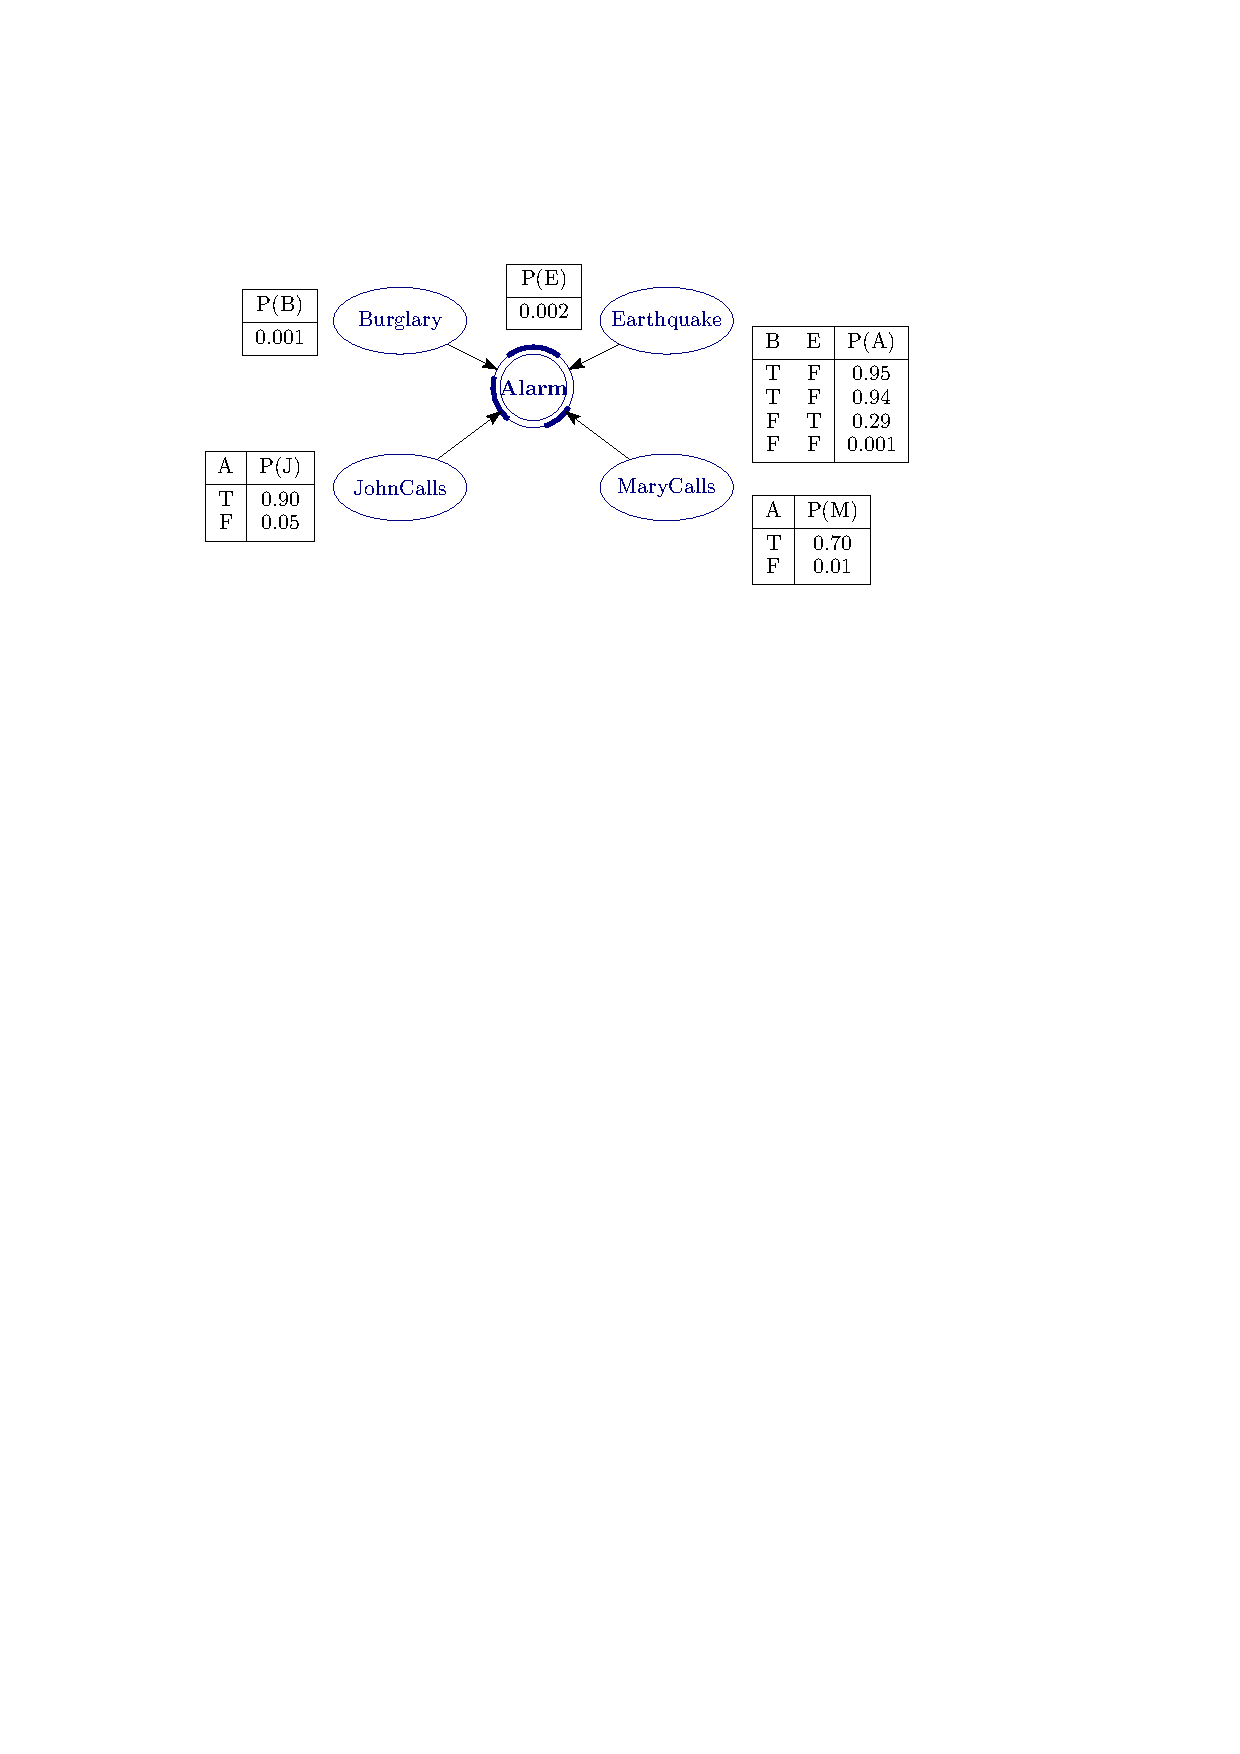
\includegraphics{image/CPT.pdf}
    \end{figure}
    在\textcolor{blue}{非因果方向}上,确定条件独立是困难的,且网络的压缩效果也不理想。
\end{definition}
\begin{note}
    贝叶斯网络(Bayesian Networks, BN)语法语义
    \begin{itemize}
        \item 全局语义:全联合概率分布与局部条件概率分布之间的关系
        \begin{figure}[htbp]
            \centering
            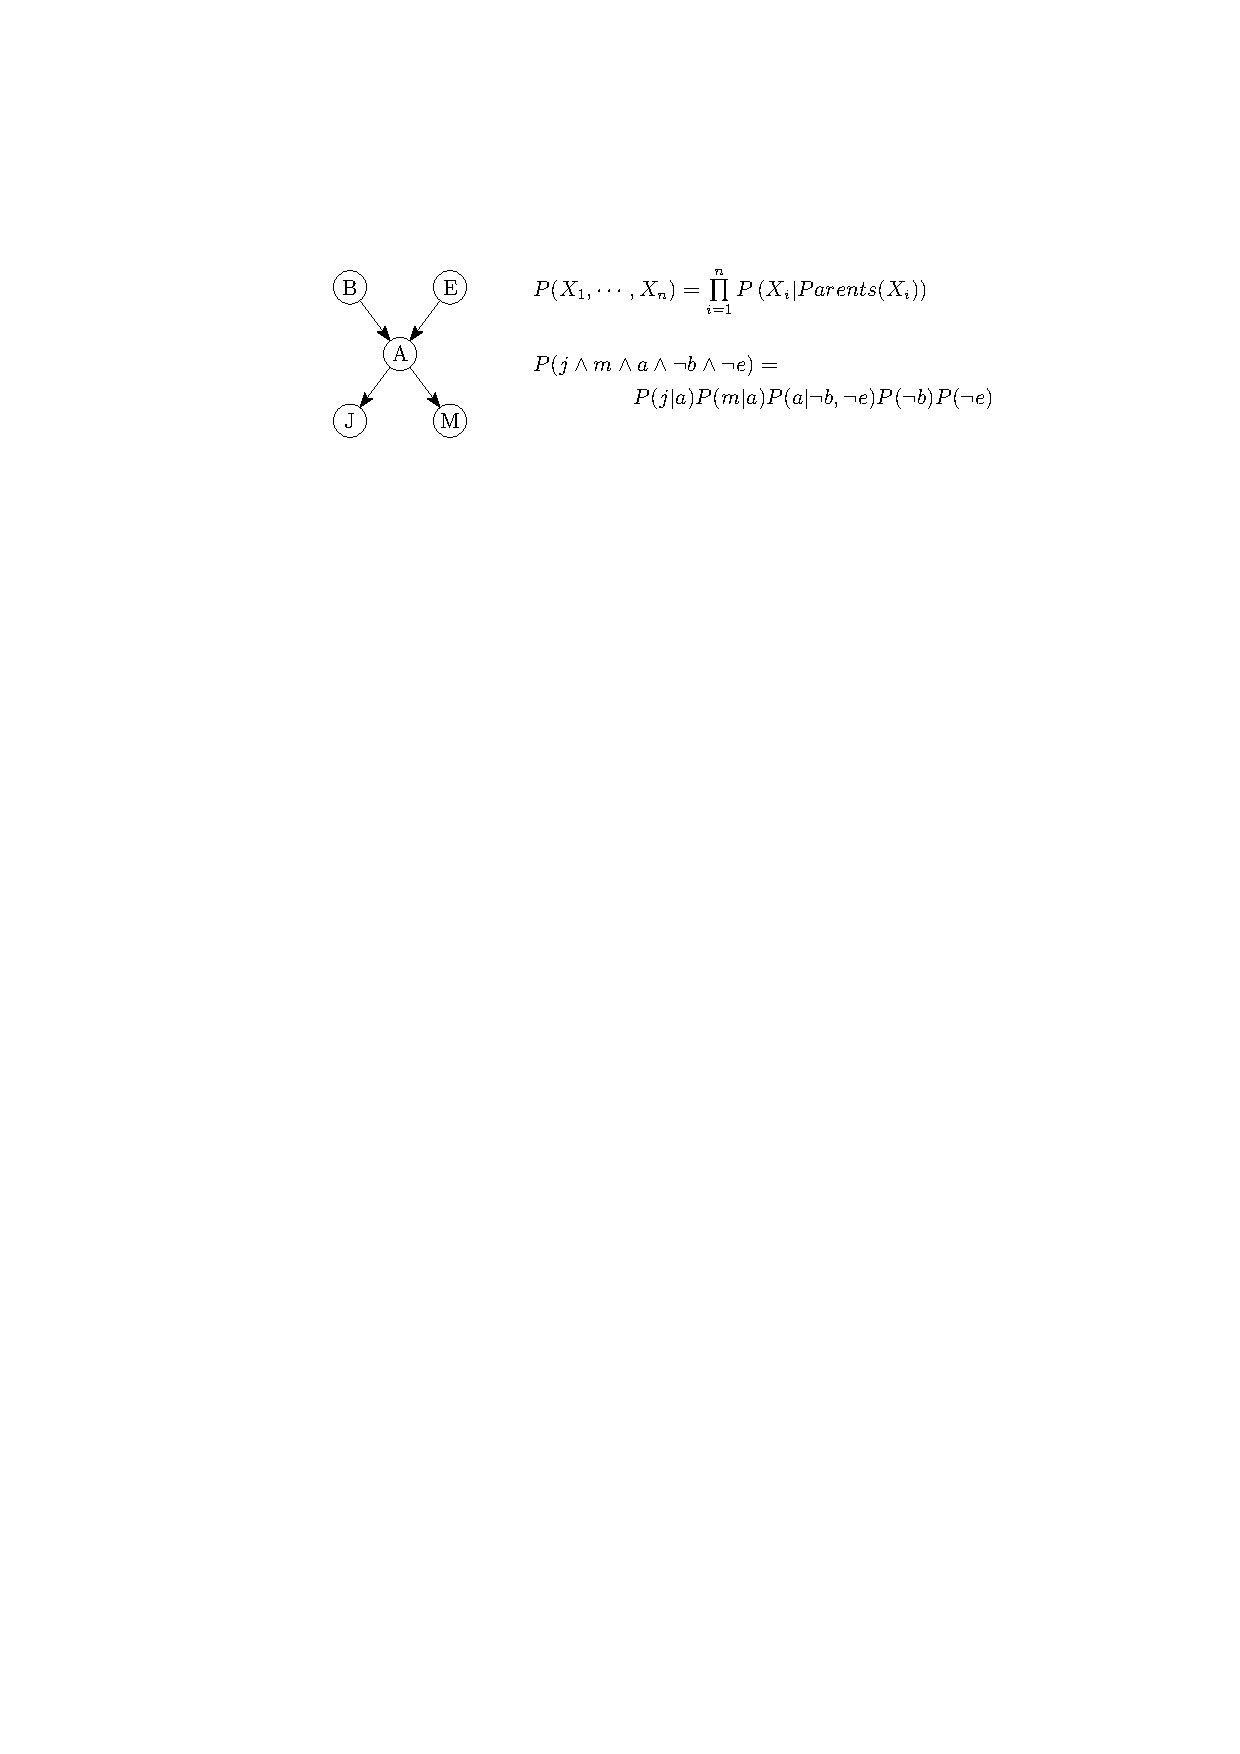
\includegraphics{image/贝叶斯网络全局语法语义.pdf}
        \end{figure}
        \item 局部语义:充分利用条件独立性,分析哪些变量之间是独立的
        
        贝叶斯网络的一个结点,如果它的父结点已知,则该结点条件独立于它的所有非后代结点
        \begin{figure}[htbp]
            \centering
            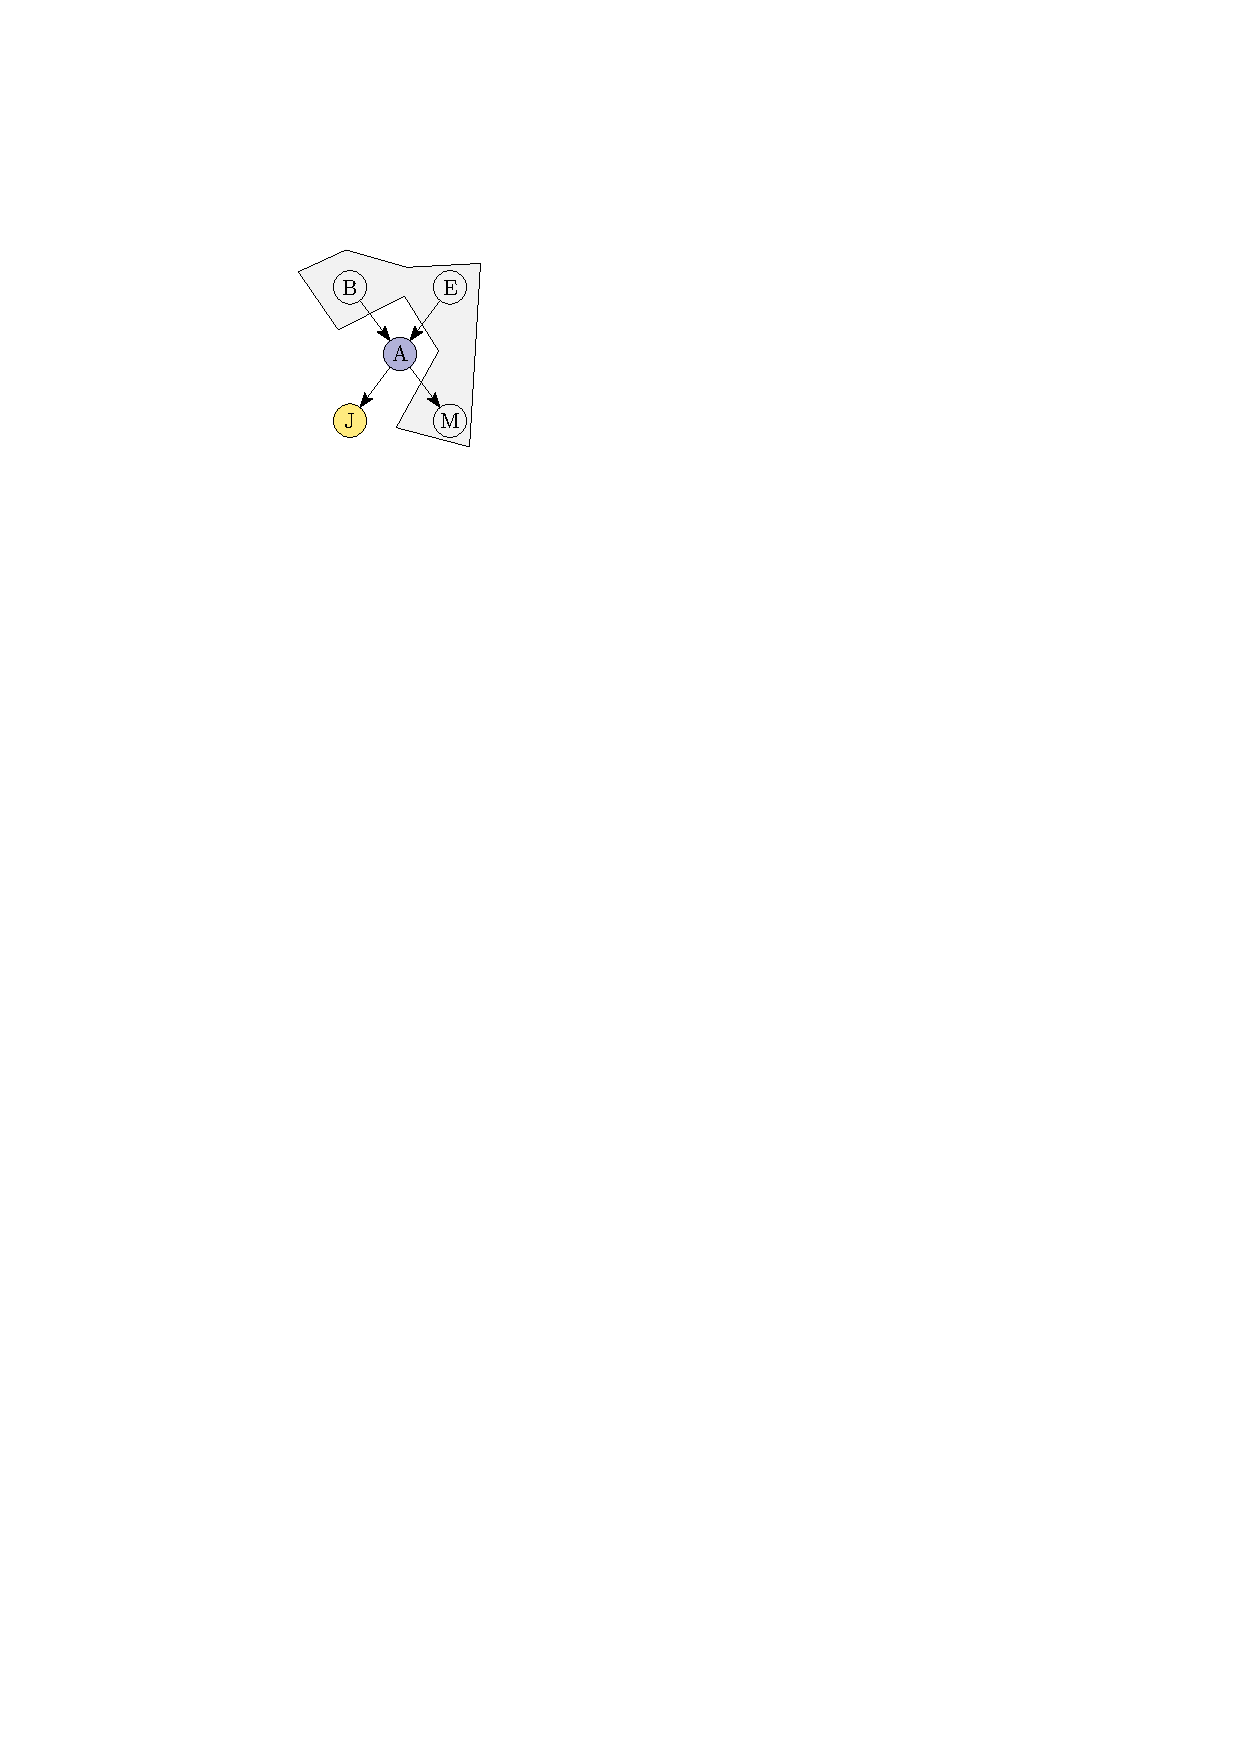
\includegraphics{image/贝叶斯网络局部语法语义.pdf}
        \end{figure}
    \end{itemize}
\end{note}
\begin{example}
    构造贝叶斯网络的步骤,主要包括:
    \begin{enumerate}[A]
        \item \textcolor{main1}{确定变量集和变量域}
        \item \textcolor{main1}{确定网络结构}
        \item \textcolor{main1}{确定节点条件概率表}
        \item 确定网络的规模
    \end{enumerate}
\end{example}
\subsubsection{基于贝叶斯网络的推理}
\begin{example}
    考虑下图所示的贝叶斯网络,解答下列问题:
    \begin{figure}[htbp]
        \centering
        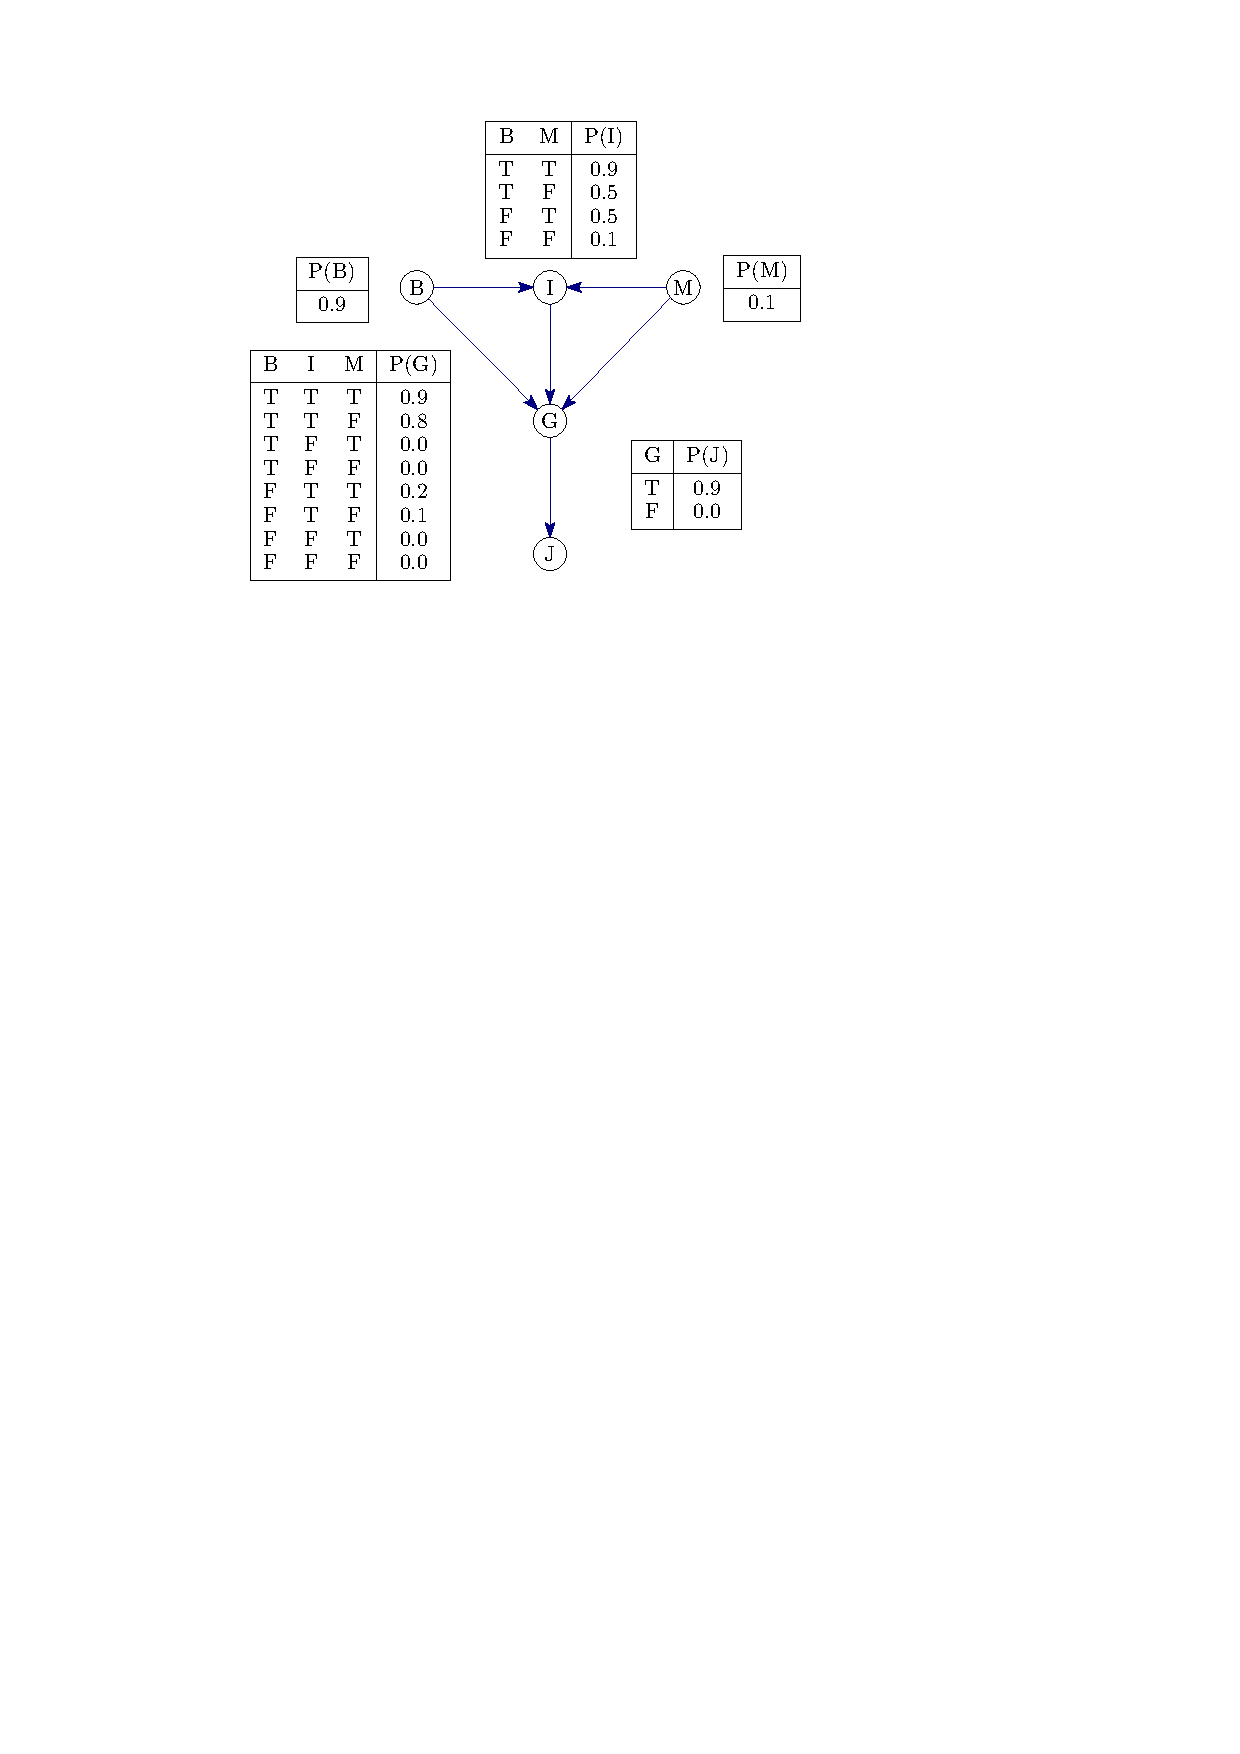
\includegraphics[scale = 0.8]{image/贝叶斯网络.pdf}
    \end{figure}
    \begin{enumerate}
        \item 网路结构能否断言下列语句?若不能,请写出正确表达式
        \begin{enumerate}
            \item $P(B,I,M) = P(B)P(I)P(M)$
            
            不能,正确表达式为$P(B,I,M) = P(I|B,M)P(B)P(M)$
            \item $P(J|G) = P(J|G,I)$
            
            能
            \item $P(M|G,B,I) = P(M|G,B,I,J)$
            
            能
        \end{enumerate}
        \item 计算$P(b,i,\lnot m,G,\lnot j)$
        \[
            \begin{array}{ll}
                &P(b,i,\lnot m,g,\lnot j) = P(\lnot j|g)P(g|b,i,\lnot m)P(i|b,\lnot m)P(b)P(\lnot m)\\
                &=(1-0.9)\times 0.8\times 0.5\times 0.9\times (1-0.1)\\
                &=0.0324
            \end{array}
        \]

        \[
            \begin{array}{ll}
                &P(b,i,\lnot m,\lnot g,\lnot j) = P(\lnot j|\lnot g)P(\lnot g|b,i,\lnot m)P(i|b,\lnot m)P(b)P(\lnot m)\\
                &=(1-0)\times (1-0.8)\times 0.5\times 0.9\times (1-0.1)\\
                &=0.081
            \end{array}
        \]
        另一种写法
        \[
            P(b,i,\lnot m,G,\lnot j) = \langle 0.0324,0.081 \rangle
        \]
    \end{enumerate}
\end{example}

\section{机器学习}
\textcolor{main1}{符号主义的困境}
\begin{figure}[htbp]
    \centering
    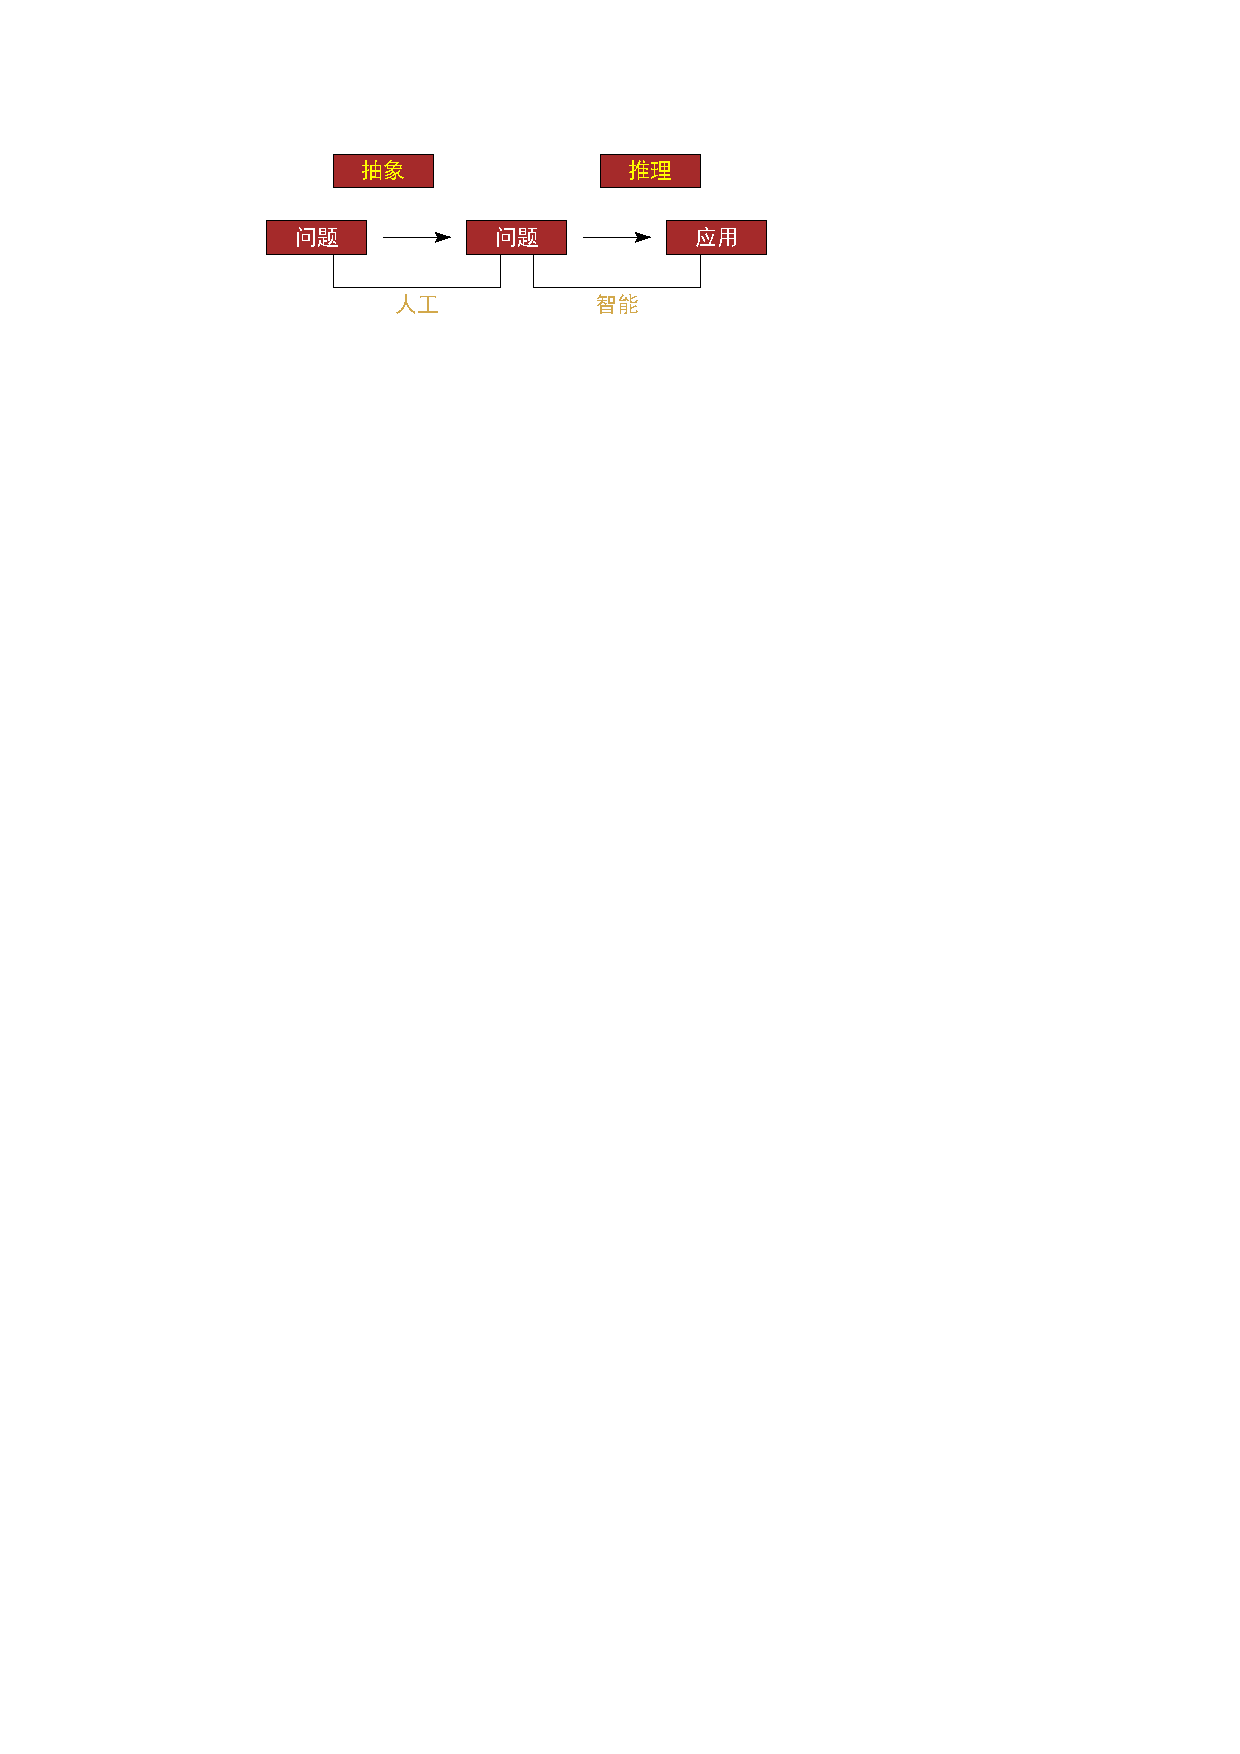
\includegraphics{image/符号主义的困境.pdf}
\end{figure}
\begin{itemize}
    \item 将问题抽象为模型的过程(知识表示)需要人工完成。把知识总结出来再交给计算机相当困难,存在知识获取瓶颈。
    \item \textcolor{main1}{很多涉及大量数据和多变量的复杂问题,没有现成的推理规则和处理方式。}
\end{itemize}

\subsection{机器学习概述}
\subsubsection{基本概念}
\textcolor{main1}{两种通用的学习类型}
\begin{figure}[htbp]
    \centering
    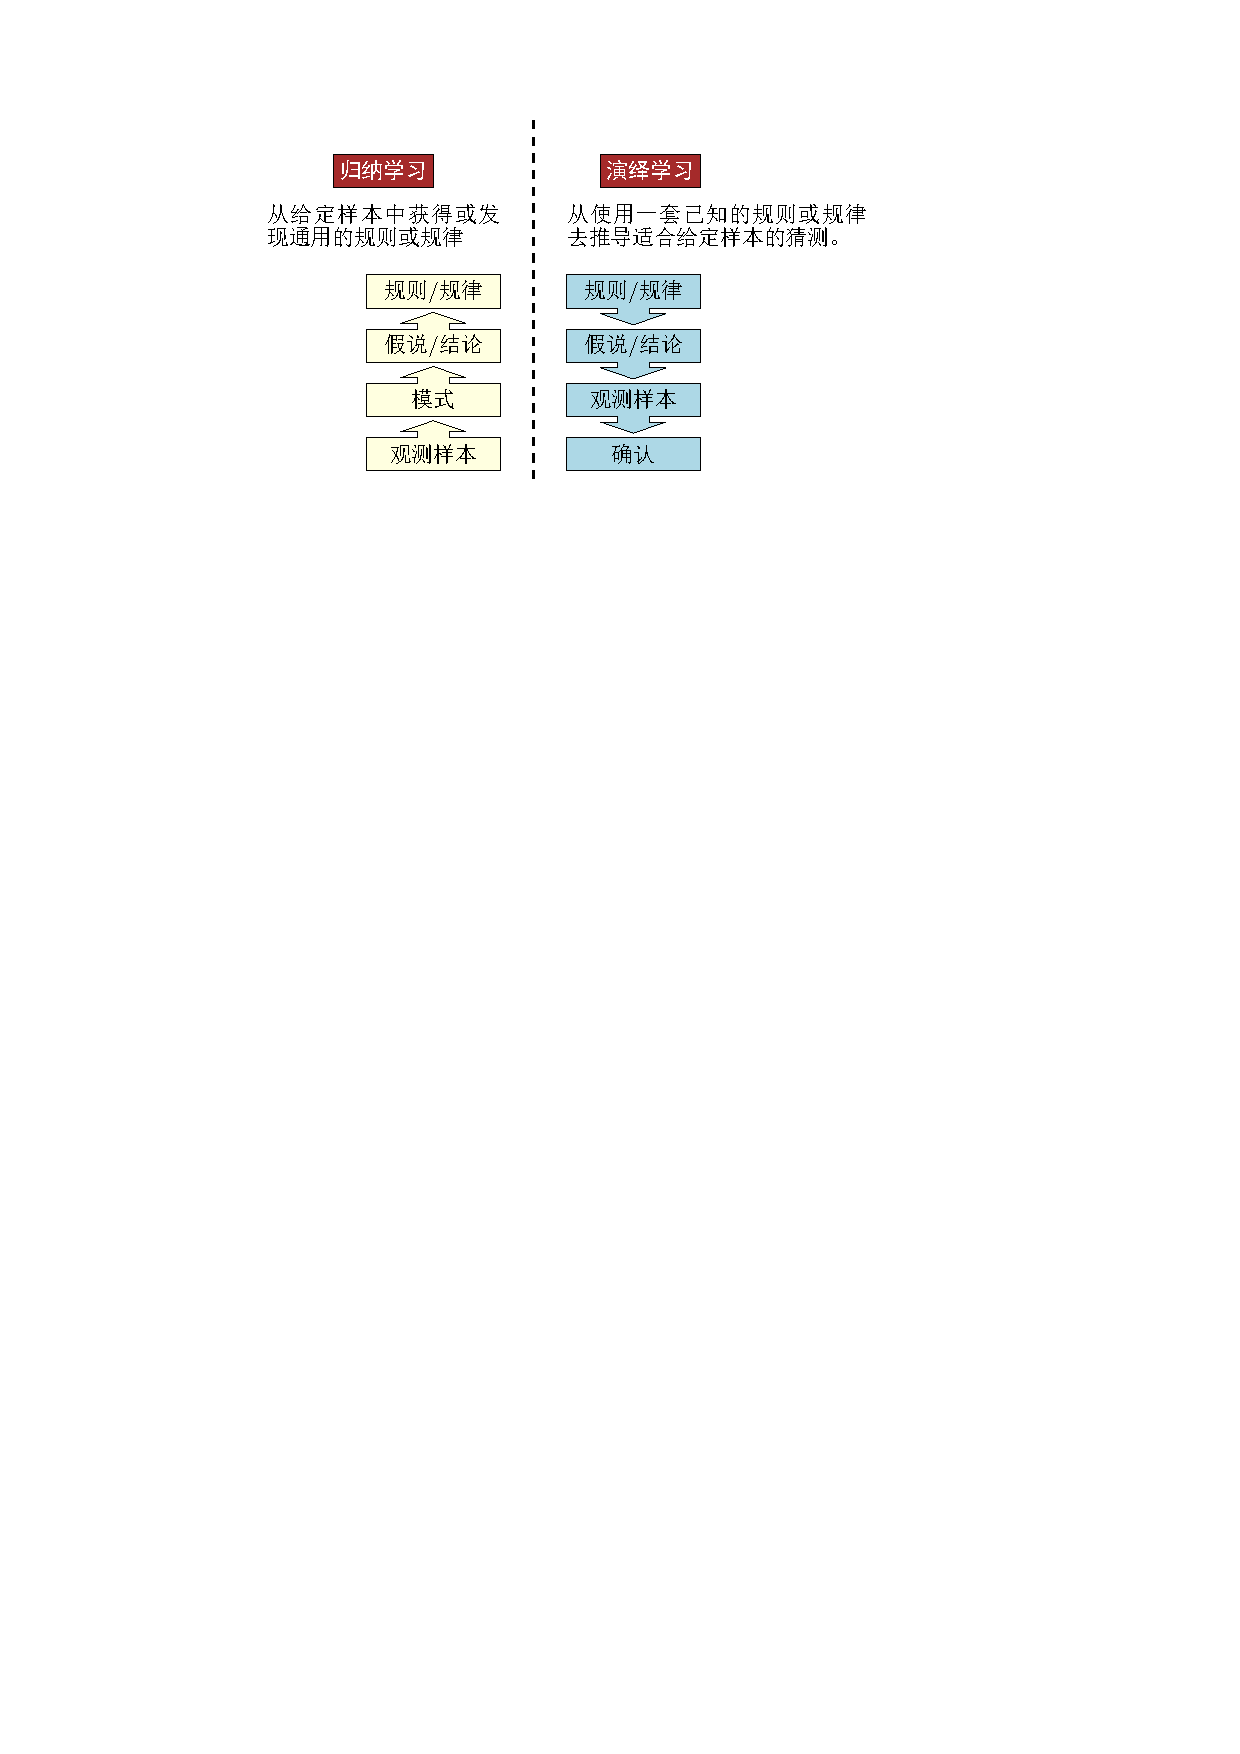
\includegraphics{image/两种通用的学习类型.pdf}
\end{figure}

\textcolor{main1}{机器学习思路}

\begin{itemize}
    \item 给定数据(样本、实例)和一定的学习规则,赋予机器自动从数据中获取知识的能力。
    \item 能够直接从样本(数据)中学习知识,不依赖于给定的判断规则。
    \item 机器学习的对象:计算机及互联网上的各种数字、文字、图像、视频、音频数据以及它们的组合。
    
    数据的基本假设是同类数据具有一定的统计规律性。
    \item 用于对数据(特别是未知数据)进行预测和分析。
\end{itemize}
\begin{figure}[htbp]
    \centering
    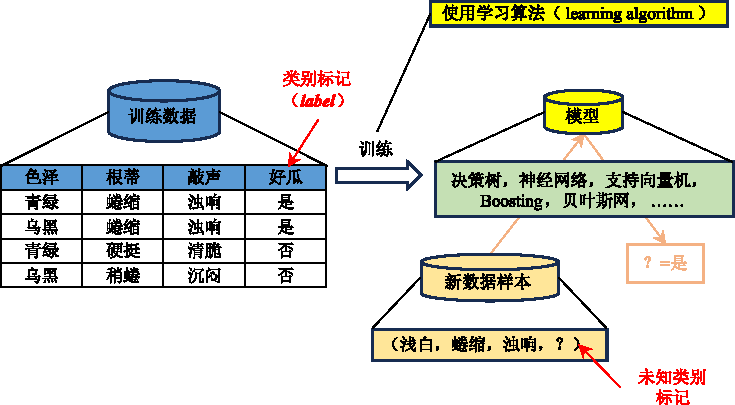
\includegraphics{image/机器学习思路.pdf}
\end{figure}
\begin{example}
    下列说法正确的是?
    \begin{enumerate}[A.]
        \item \textcolor{main1}{机器学习从数据中自动分析并获得规律}
        \item 机器学习中所采用的判断规则是事先给定的
        \item 利用已有公式可以计算的问题需要使用机器学习
        \item \textcolor{main1}{机器学习适于解决数据丰富且规则不明确的问题}
    \end{enumerate}
\end{example}
\textcolor{main1}{机器学习的数据}
\begin{itemize}
    \item \textcolor{main1}{样本:}关于一个对象或事件描述的一条记录
    \item \textcolor{main1}{特征(属性):}反映对象或事件在某方面的表现或性质
    \item \textcolor{main1}{标签:}样本标注的类别信息(离散)或者程度信息(连续),也可能没有。
\end{itemize}
\textcolor{main1}{归纳偏好}

机器学习算法在学习过程中对某种类型假设的偏好。
\begin{figure}[htbp]
    \centering
    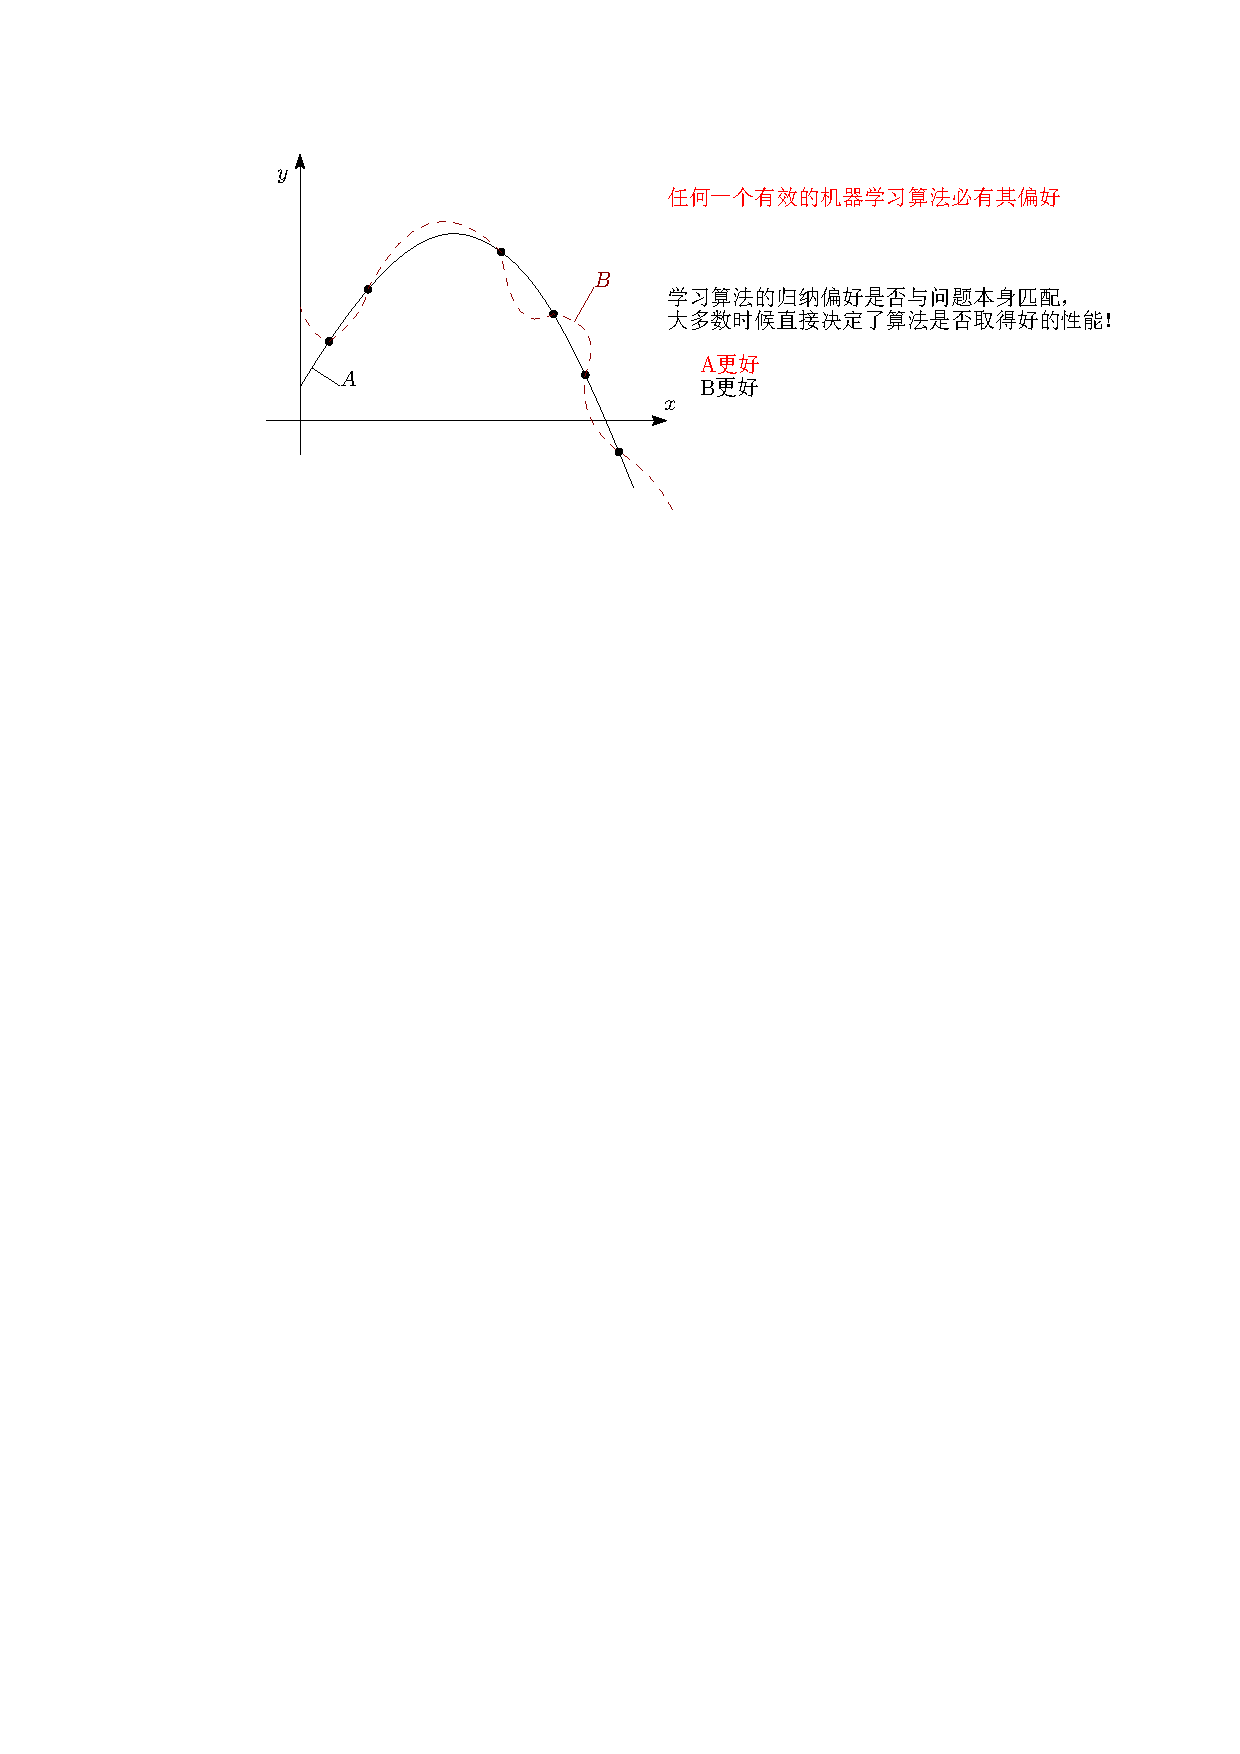
\includegraphics{image/归纳偏好.pdf}
\end{figure}

\textcolor{main1}{NFL(No Free Lunch)定理}

\begin{theorem}[NFL定理]
    一个算法A若在某些问题上比另一个算法B好,必存在另一些问题B比A好。
\end{theorem}
\begin{figure}[htbp]
    \centering
    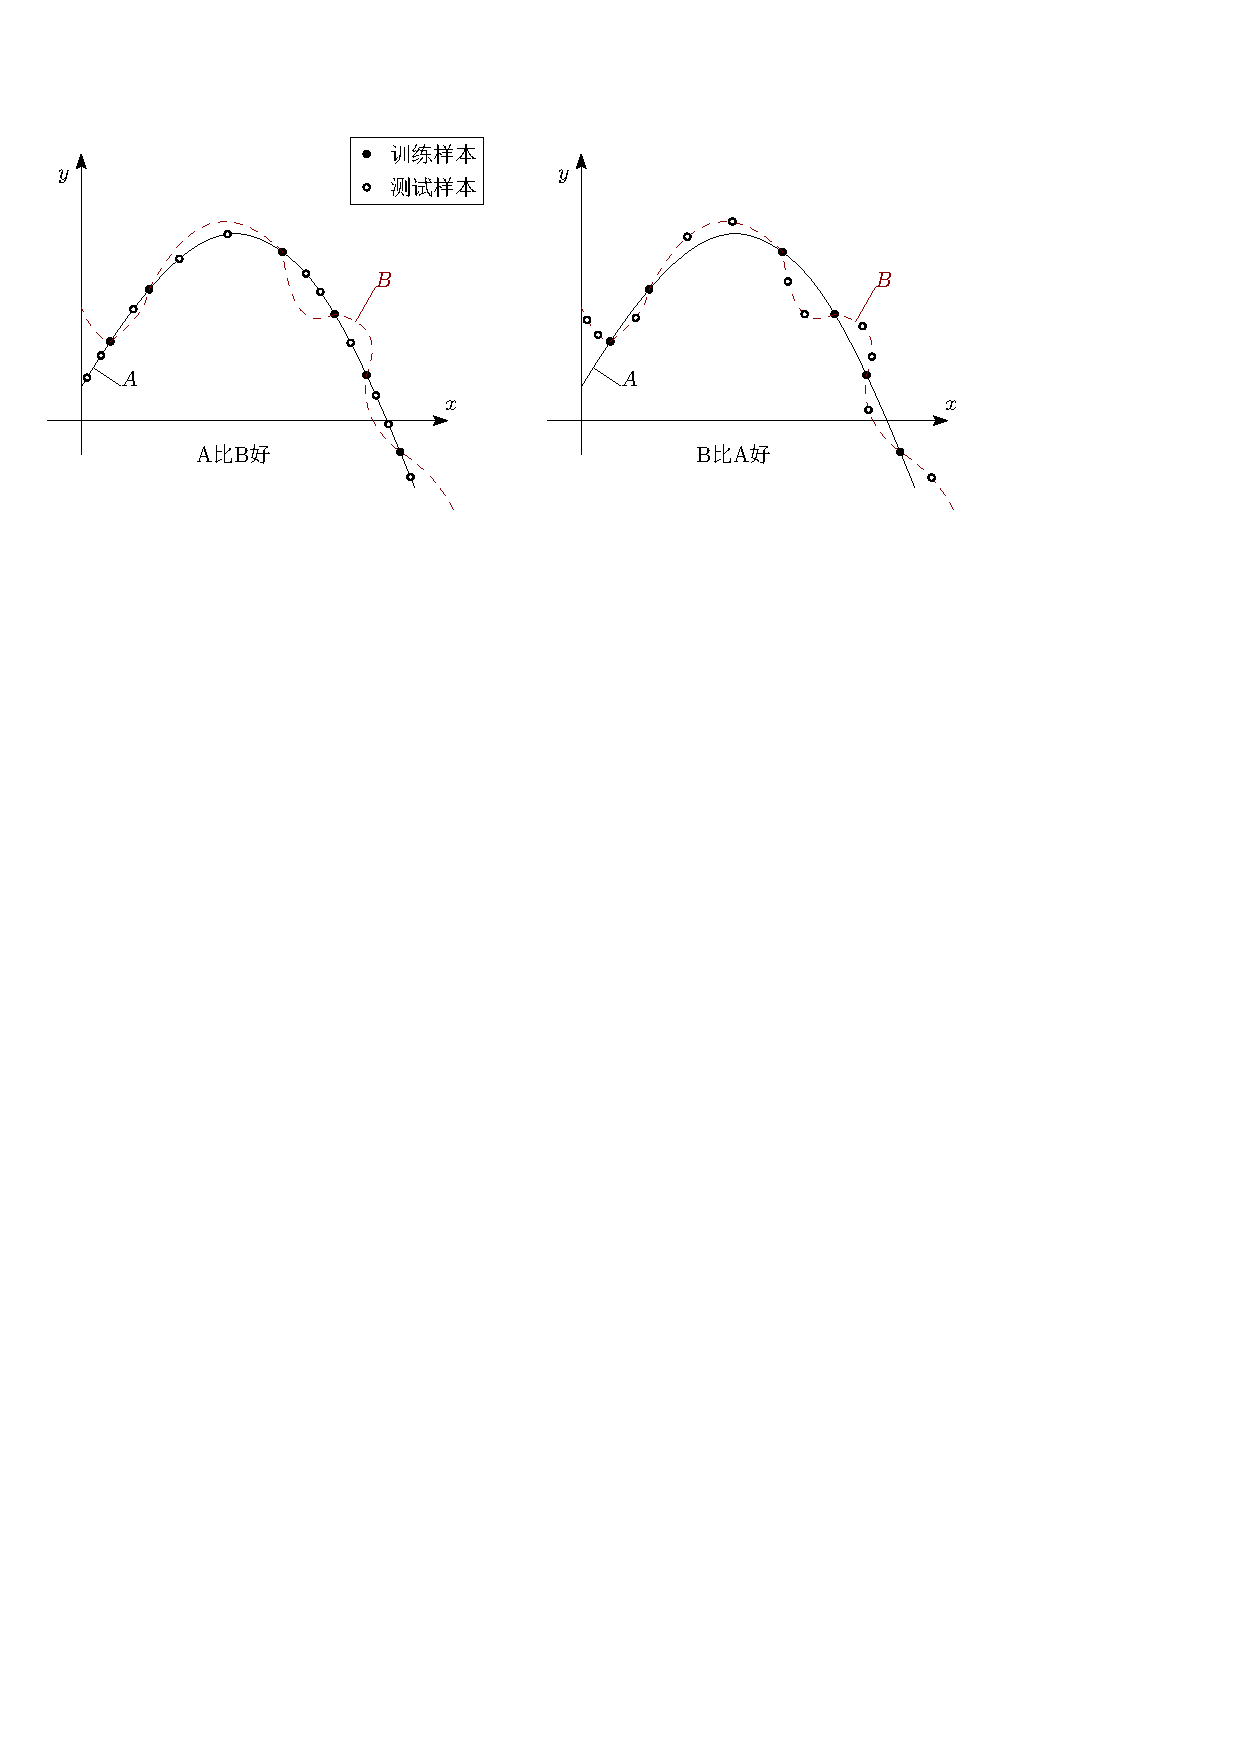
\includegraphics{image/NFL.pdf}
\end{figure}

\begin{definition}[泛化能力]
    机器学习的目标是使得学到的模型能很好的适用于“新样本”而不仅仅是训练集合,模型适用于新样本的能力被称为\textcolor{main1}{泛化(Generalization)能力}。
\end{definition}

\begin{figure}[htbp]
    \centering
    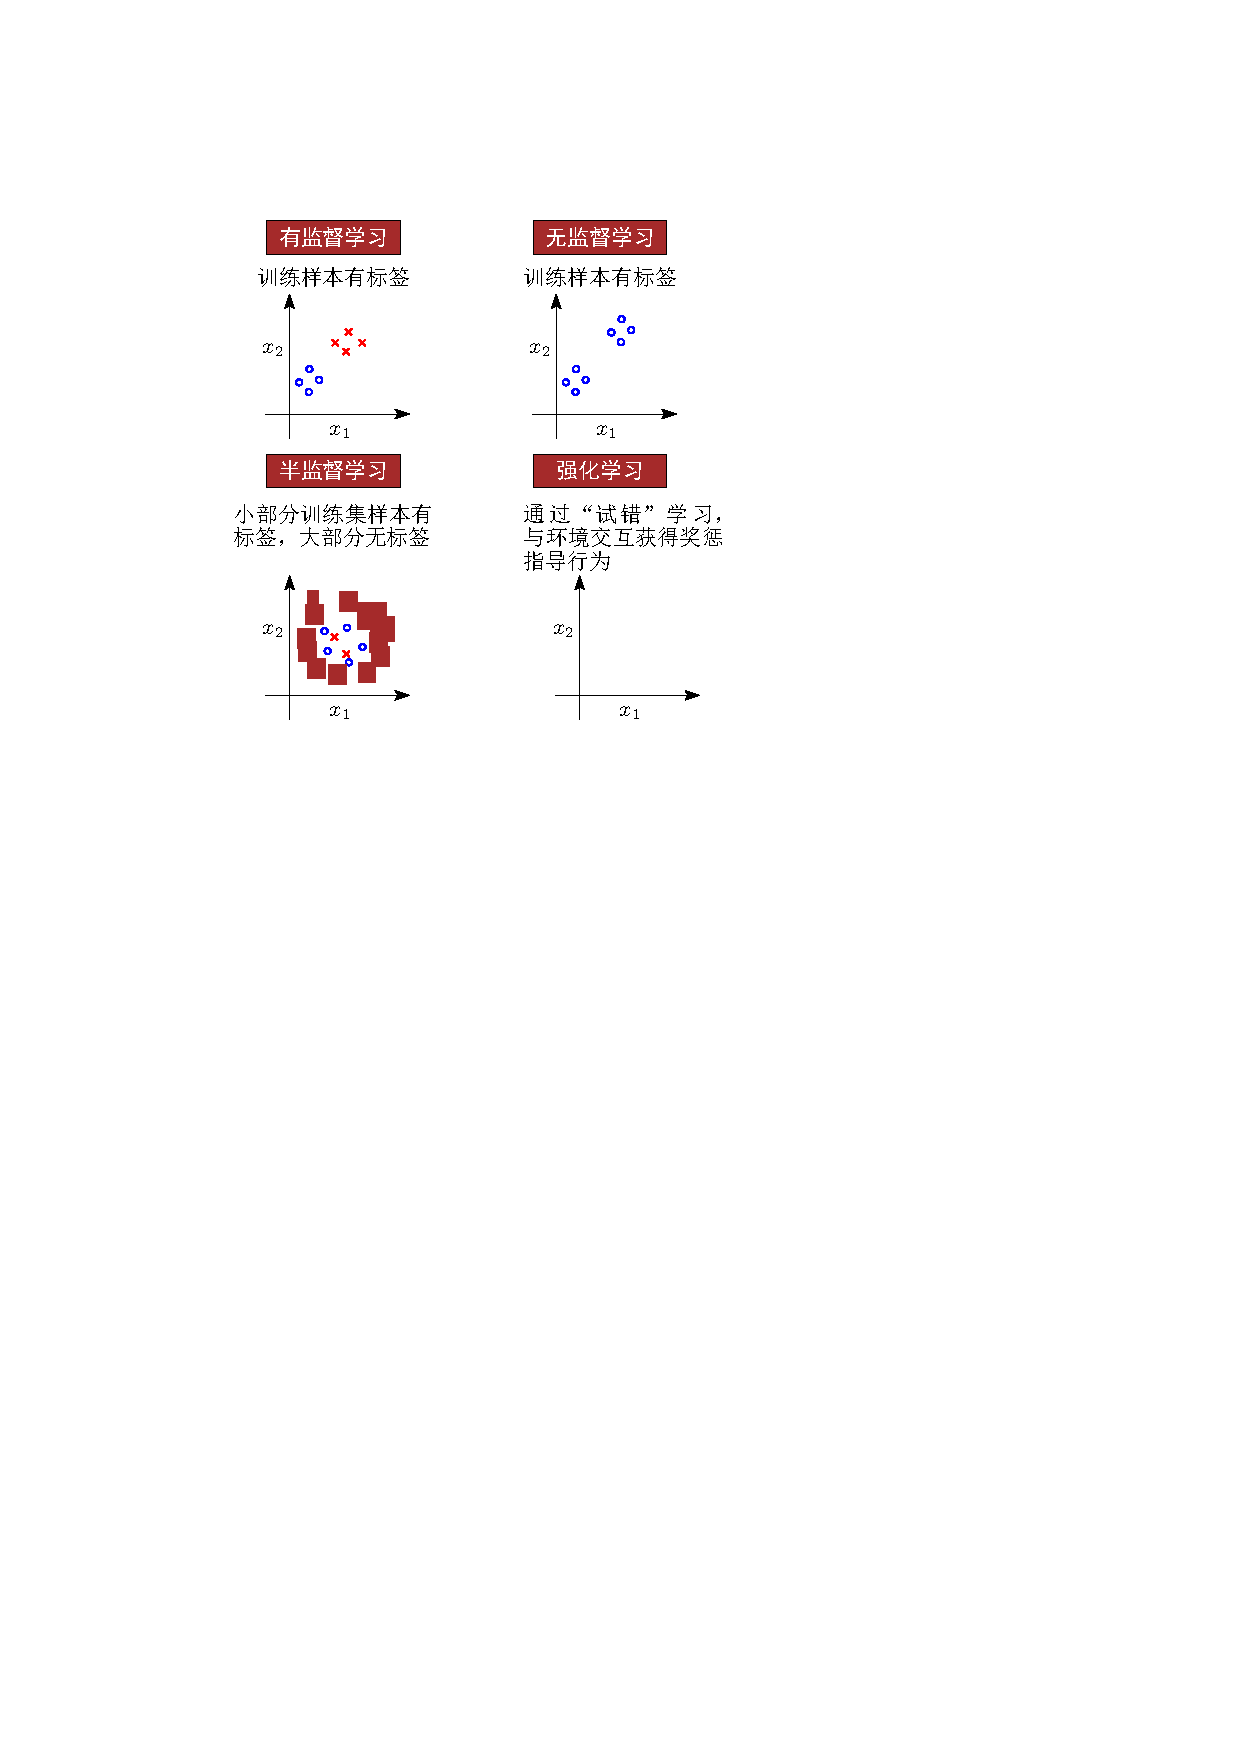
\includegraphics{image/机器学习的分类.pdf}
\end{figure}

\textcolor{main1}{强化学习vs. 有监督学习}
\begin{itemize}
    \item 相似点:
    \begin{enumerate}
        \item 强化学习中“状态”对应监督学习中的“示例”、“动作”对应“标签”,“策略”相当于“分类器”或“回归器”
        \item 强化学习中没有(监督学习中的那种)有标签样本(即“示例-标签”),换言之,没有人告诉机器在什么状态下应该做什么,而是通过最终结果“反思”之前的动作是否正确来进行学习
        \item 因此,强化学习在某种意义上可以看成具有“延迟标签信息”的监督学习问题
    \end{enumerate} 
    \item 不同点
    \begin{enumerate}
        \item 有监督学习的训练样本是有标签的,强化学习的训练是没有标签的,只有环境给出的奖惩
        \item 有监督学习的学习过程是静态的,不与环境进行交互,给什么样本就学什么。强化学习的学习过程是动态的,与环境进行交互,通过环境给出奖惩来学习。
        \item 有监督学习主要感觉感知问题,强化学习主要解决决策问题。
    \end{enumerate}
\end{itemize}
\begin{example}
    下面关于有监督学习说法正确的是?
    \begin{enumerate}[A]
        \item \textcolor{main1}{通过已知的训练样本来训练}
        \item \textcolor{main1}{训练样本是带有标签的}
        \item 对于训练集之外的样本,学习到的模型不能够预测结果
        \item \textcolor{main1}{可以应用于目标识别中}
    \end{enumerate}
\end{example}
\subsection{有监督学习基本方法}
回归和分类取决于训练用的标签是连续还是离散的,它们预测获得标签也对应的是连续和离散的。

\textcolor{main1}{有监督学习的一般过程}
\begin{itemize}
    \item 数据准备
    \begin{itemize}
        \item 如果问题是全新的 ,采集或爬取带标签的数据;如果数据仓库有相应的数据,将数据提取出来。
        \item 数据准备好之后,需要对数据进行预处理,主要包括重复数据检测、数据标准化、数据编码、缺失值处理、异常值处理等。
    \end{itemize}
    \item 特征选择或抽取
    \begin{itemize}
        \item 特征选择:选取原始特征集合的有效子集,保留有用特征,移除冗余或无关的特征。
        \item 特征抽取:构造一个新的特征空间,将原始特征投影到新的空间中表示。
    \end{itemize}
    \item 训练——从数据中学习获得模型的过程,包括选择模型和确定参数。
    \begin{itemize}
        \item 超参数,如深度学习模型中各层的神经元数量;
        \item 模型内部参数,如深度学习模型中神经元间的连接权值。
    \end{itemize}
    \item 验证/测试——选取一部分已知类别的样本评估模型分类效果
    \begin{itemize}
        \item 误差:模型输出与真值的偏离程度
        \item 训练 (经验) 误差:模型在训练集上的误差
        \item 测试误差:模型在测试集上的误差
        \item 泛化误差:在除训练集外所有样本上的误差
    \end{itemize}
    \begin{note}
        验证/测试的注意:
        \begin{itemize}
            \item 假设测试集是从样本真实分布中独立采样获得,将测试集上的“测试误差”作为泛化误差的近似,所以测试集要和训练集中的样本互斥。
            \item 独立测试集:选择与训练样本相独立的数据集进行验证,评估模型的分类效果。
            \item 交叉验证:将原始数据分组,大部分作为训练集,进行训练模型;另一部分作为验证集,测试训练得到的模型的正确率,用来调整模型参数。k 折交叉验证是将原始数据分为k 组,每次留1 组作为验证集。特例:留1 法。
        \end{itemize}
    \end{note}
    \item K折交叉验证(K-fold cross-validation)
    \begin{figure}[htbp]
        \centering
        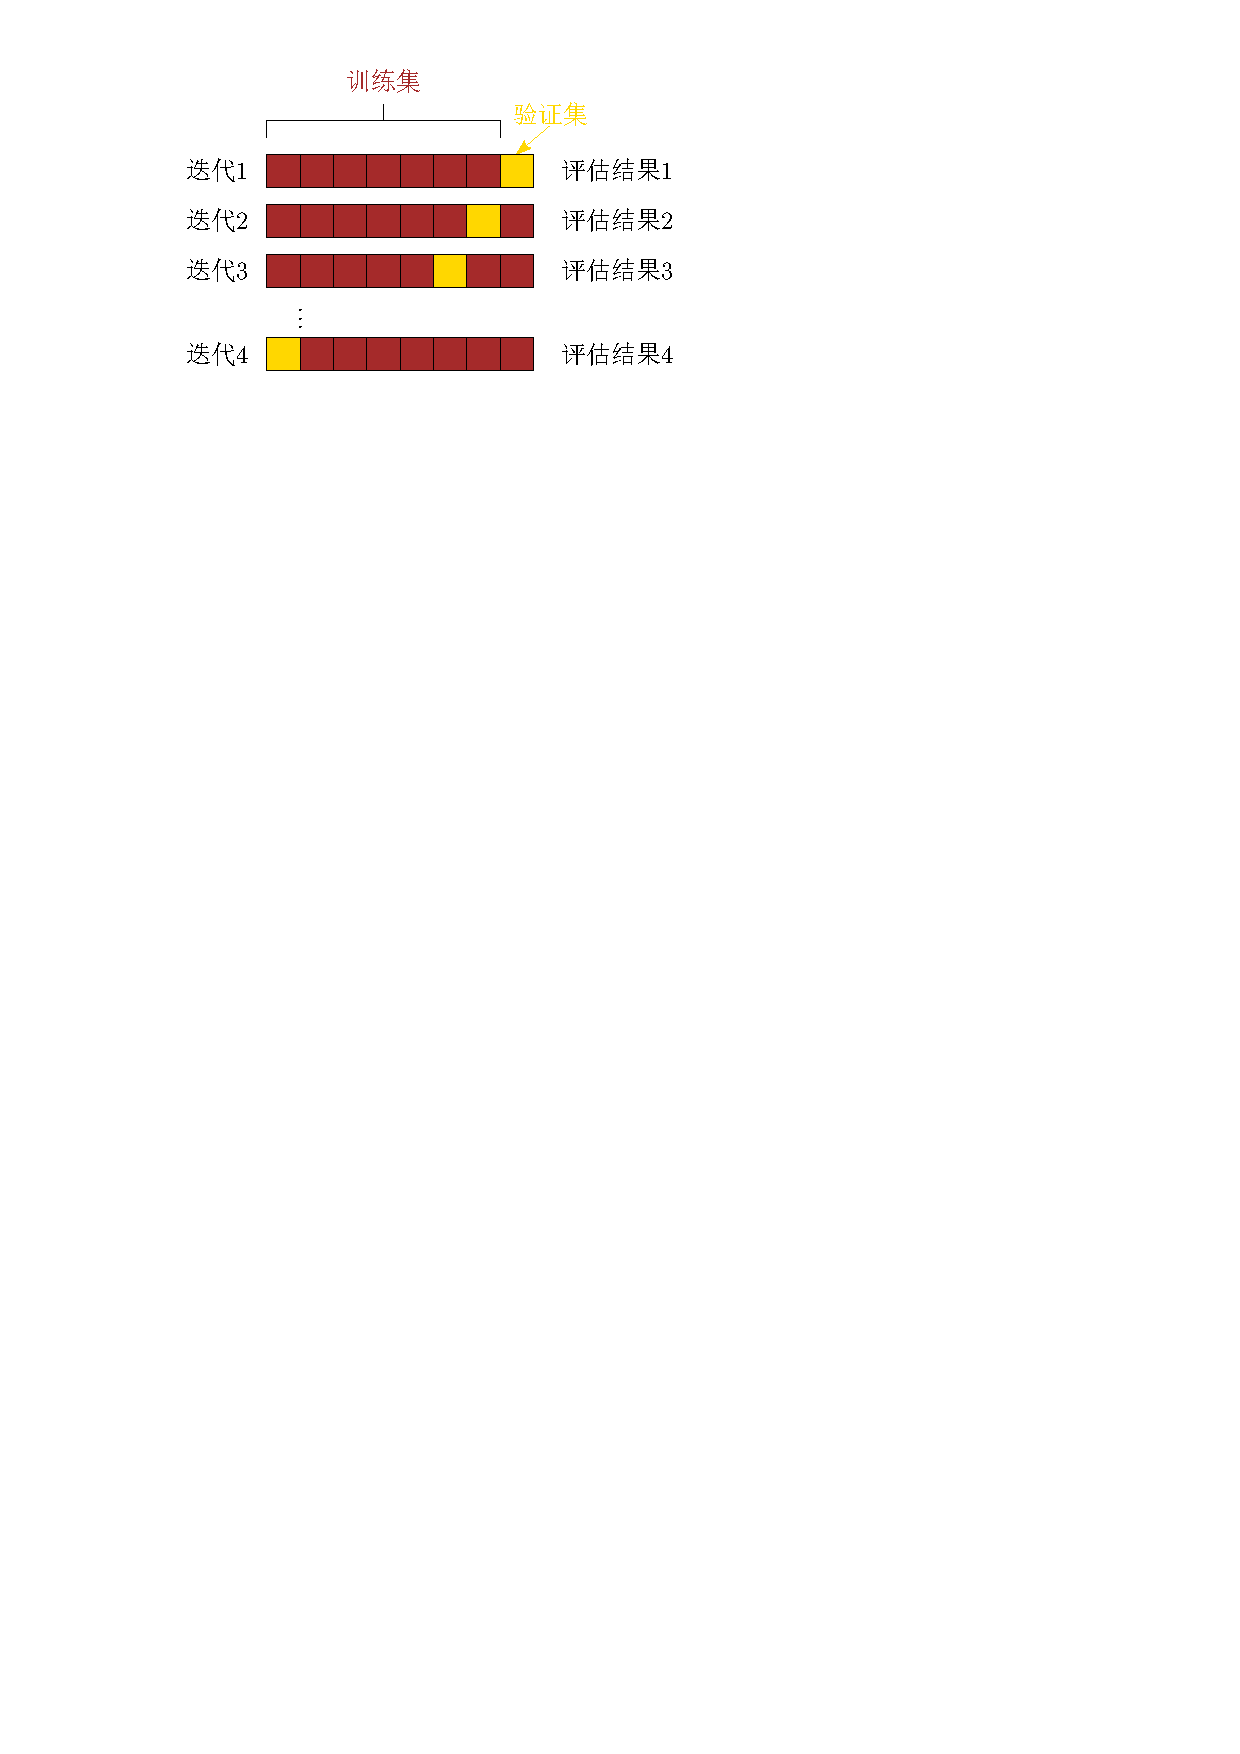
\includegraphics{image/K折交叉验证.pdf}
    \end{figure}
    \begin{itemize}
        \item 初始采样分割成K个子样本,一个单独的子样本被保留作为验证模型的数据,其他K-1个样本用来训练。
        \item 交叉验证重复K次,每个子样本验证一次,最终得到一个单一估测。
        \item 这个方法的优势在于,同时重复运用随机产生的子样本进行训练和验证,每次的结果验证一次,10折交叉验证是最常用的。
    \end{itemize}
\end{itemize}
\begin{example}
    思考题:
    \begin{enumerate}
        \item 训练数据、验证数据可以有交叠吗?
        
        不能有交叠。
        \item 为什么要进行交叉验证,随机选取其中一部分只做一次测试好不好?
        
        多次交叉验证的效果更好,可以充分利用已知数据计算出多个预测正确率,获得最终预测正确率的平均值和方差,更准确地评估模型的预测效果。
    \end{enumerate}
\end{example}
\begin{example}
    影响有监督学习性能的因素有哪些?
    \begin{enumerate}[A]
        \item \textcolor{main1}{可用数据的样本规模}
        \item \textcolor{main1}{数据预处理}
        \item \textcolor{main1}{特征抽取与选择}
        \item \textcolor{main1}{机器学习算法设计}
    \end{enumerate}
\end{example}
\subsubsection{回归问题}
\textcolor{main1}{最小二乘法}

回归方程:$\hat{y} = f(x) = \boldsymbol{x}^{\mathrm{T}}\boldsymbol{w} + b$

\[
    \begin{array}{ll}
        (\boldsymbol{w}^{*},b^{*}) &= \arg\min\limits_{(\boldsymbol{w},b)}\sum_{i = 1}^{m}\left( f(x_i)-y_i \right)^2\\
        &= \arg\min\limits_{(\boldsymbol{w},b)}\sum_{i = 1}^{m}\left( y_i - \boldsymbol{x}_i^{\mathrm{T}}\boldsymbol{w} - b \right)^2
    \end{array}
\]
\[
    Q = \sum_{i = 1}^{m}\left( y_i - \boldsymbol{w}^{\mathrm{T}}\boldsymbol{x}_i - b \right)^2 = (\boldsymbol{y}-\boldsymbol{X}\hat{\boldsymbol{w}})^{\mathrm{T}} (\boldsymbol{y}-\boldsymbol{X}\hat{\boldsymbol{w}})
\]
其中,$\boldsymbol{X}$和$\hat{\boldsymbol{w}}$为
\[
    \boldsymbol{X} = \begin{bmatrix}
        \boldsymbol{x}_1^{\mathrm{T}} & 1\\
        \vdots & \vdots \\
        \boldsymbol{x}_m^{\mathrm{T}} & 1\\
    \end{bmatrix},\,
    \hat{\boldsymbol{w}} = \begin{bmatrix}
        \boldsymbol{w}\\
        b
    \end{bmatrix} 
\]
求其偏导数并令其为$\boldsymbol{0}$,即:
\[
    \begin{array}{c}
        \dfrac{\partial Q}{\partial \hat{\boldsymbol{w}}} = 2\boldsymbol{X}^{\mathrm{T}}\boldsymbol{Xw}-2\boldsymbol{X}^{\mathrm{T}}\boldsymbol{y} = \boldsymbol{0}\\
        \hat{\boldsymbol{w}} = \left( \boldsymbol{X}^{\mathrm{T}}\boldsymbol{X} \right)^{-1}\boldsymbol{X}^{\mathrm{T}}\boldsymbol{y}
    \end{array}
\]

\begin{example}
    \textcolor{main1}{改进线性回归问题性能的方法包括}
    \begin{enumerate}[A]
        \item \textcolor{main1}{引入新的特征}
        \item \textcolor{main1}{提高多项式模
        型的阶次}
        \item \textcolor{main1}{选择合适的曲线回归模型}
        \item \textcolor{main1}{抽取更有效的特征}
    \end{enumerate}
\end{example}

\textcolor{main1}{非线性回归}
\begin{definition}[非线性回归]
    两种回归通过在目标函数中引入\textcolor{main1}{正则化项}来处理\textcolor{main1}{多重共线性问题},并达到防止过拟合的目的。岭回归采用的是L2正则化,
而Lasso回归采用的是L1正则化。    
\end{definition}
\begin{figure}[htbp]
    \centering
    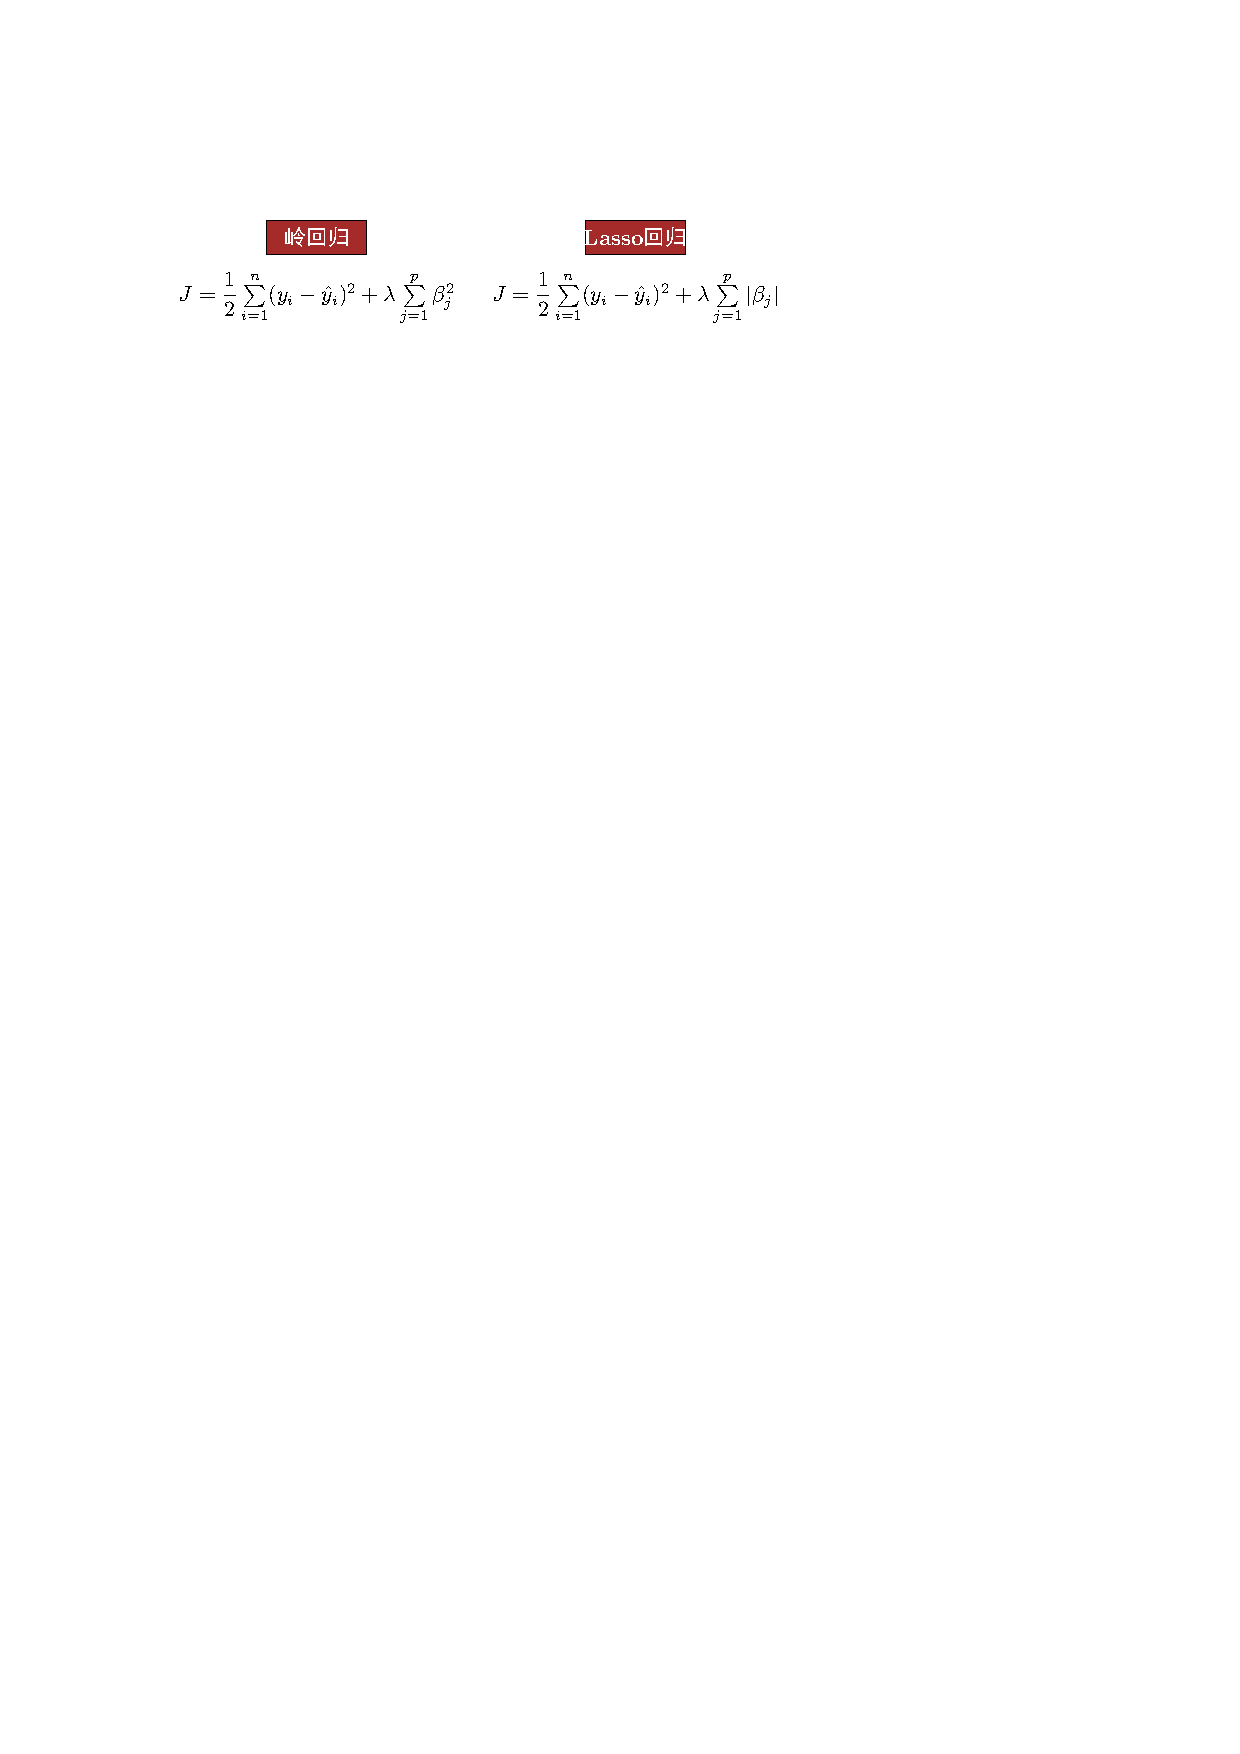
\includegraphics{image/非线性回归.pdf}
\end{figure}

\subsubsection{分类问题}
\begin{definition}[分类问题]
    分类也是有监督学习的一种。它解决的是样本的标签是离散值的情况,其试图给出的预测值也是离散的。
    \begin{itemize}
        \item \textcolor{main1}{二分类问题:}非此即彼的分类问题,输出值,0或1,0代表不合格,1代表合格
        \item \textcolor{main1}{多分类问题:}如分四等次,对应预测离散输出值为0、1、2、3。0代表不及格、1表示及格、2表示良好、3表示优秀。
    \end{itemize}
\end{definition}

\begin{example}
    能否将分类问题的标签作为输出值直接利用回归算法求解?
    \begin{enumerate}[A]
        \item 能
        \item \textcolor{main1}{不能}
    \end{enumerate}
\end{example}

\textcolor{main1}{分类问题性能度量}

衡量模型泛化能力的评价标准,反映了任务需求,使用不同的性能度量往往会导致不同的评判结果。
\begin{itemize}
    \item  在对于分类任务,错误率和准确率是最常用的两种性能度量:
    \begin{itemize}
        \item 分类错误率:分错样本占样本总数的比例
        \[
            E(f;D) = \dfrac{1}{m}\sum_{i = 1}^{m}I_{f(x_i)\neq y_i}
        \]
        \item 分类准确率:分对样本占样本总数的比例
        \[
            acc(f;D) = \dfrac{1}{m}\sum_{i = 1}^{m}I_{f(x_i)= y_i} = 1-E(f;D)
        \]
        \item 诊断、检测等应用场景中,查准率和查全率比分类错误率和分类精度更适合。
        \begin{figure}[htbp]
            \centering
            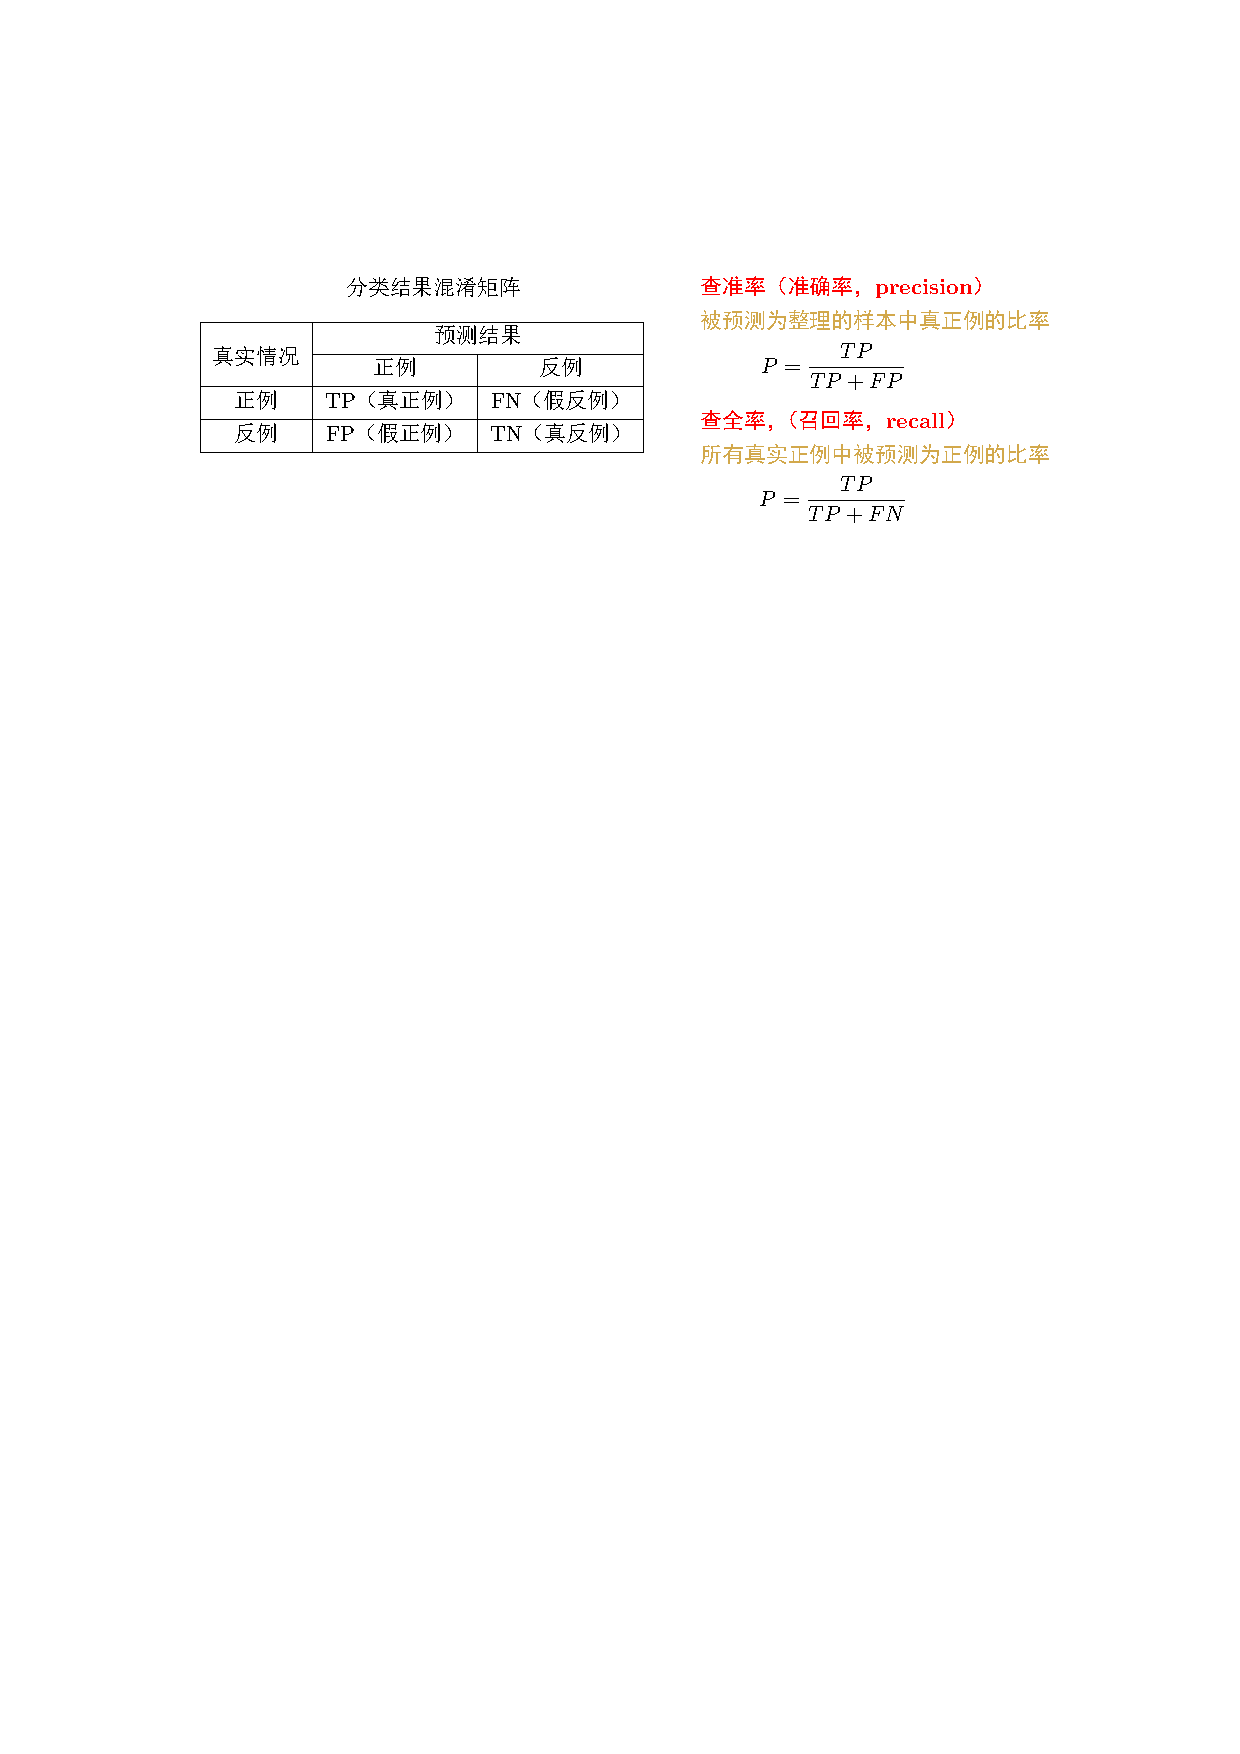
\includegraphics{image/混淆矩阵.pdf}
        \end{figure}

        查准率和查全率是一对矛盾的度量。
    \end{itemize}
\end{itemize}

\textcolor{main1}{线性判别分析}
\begin{figure}[htbp]
    \centering
    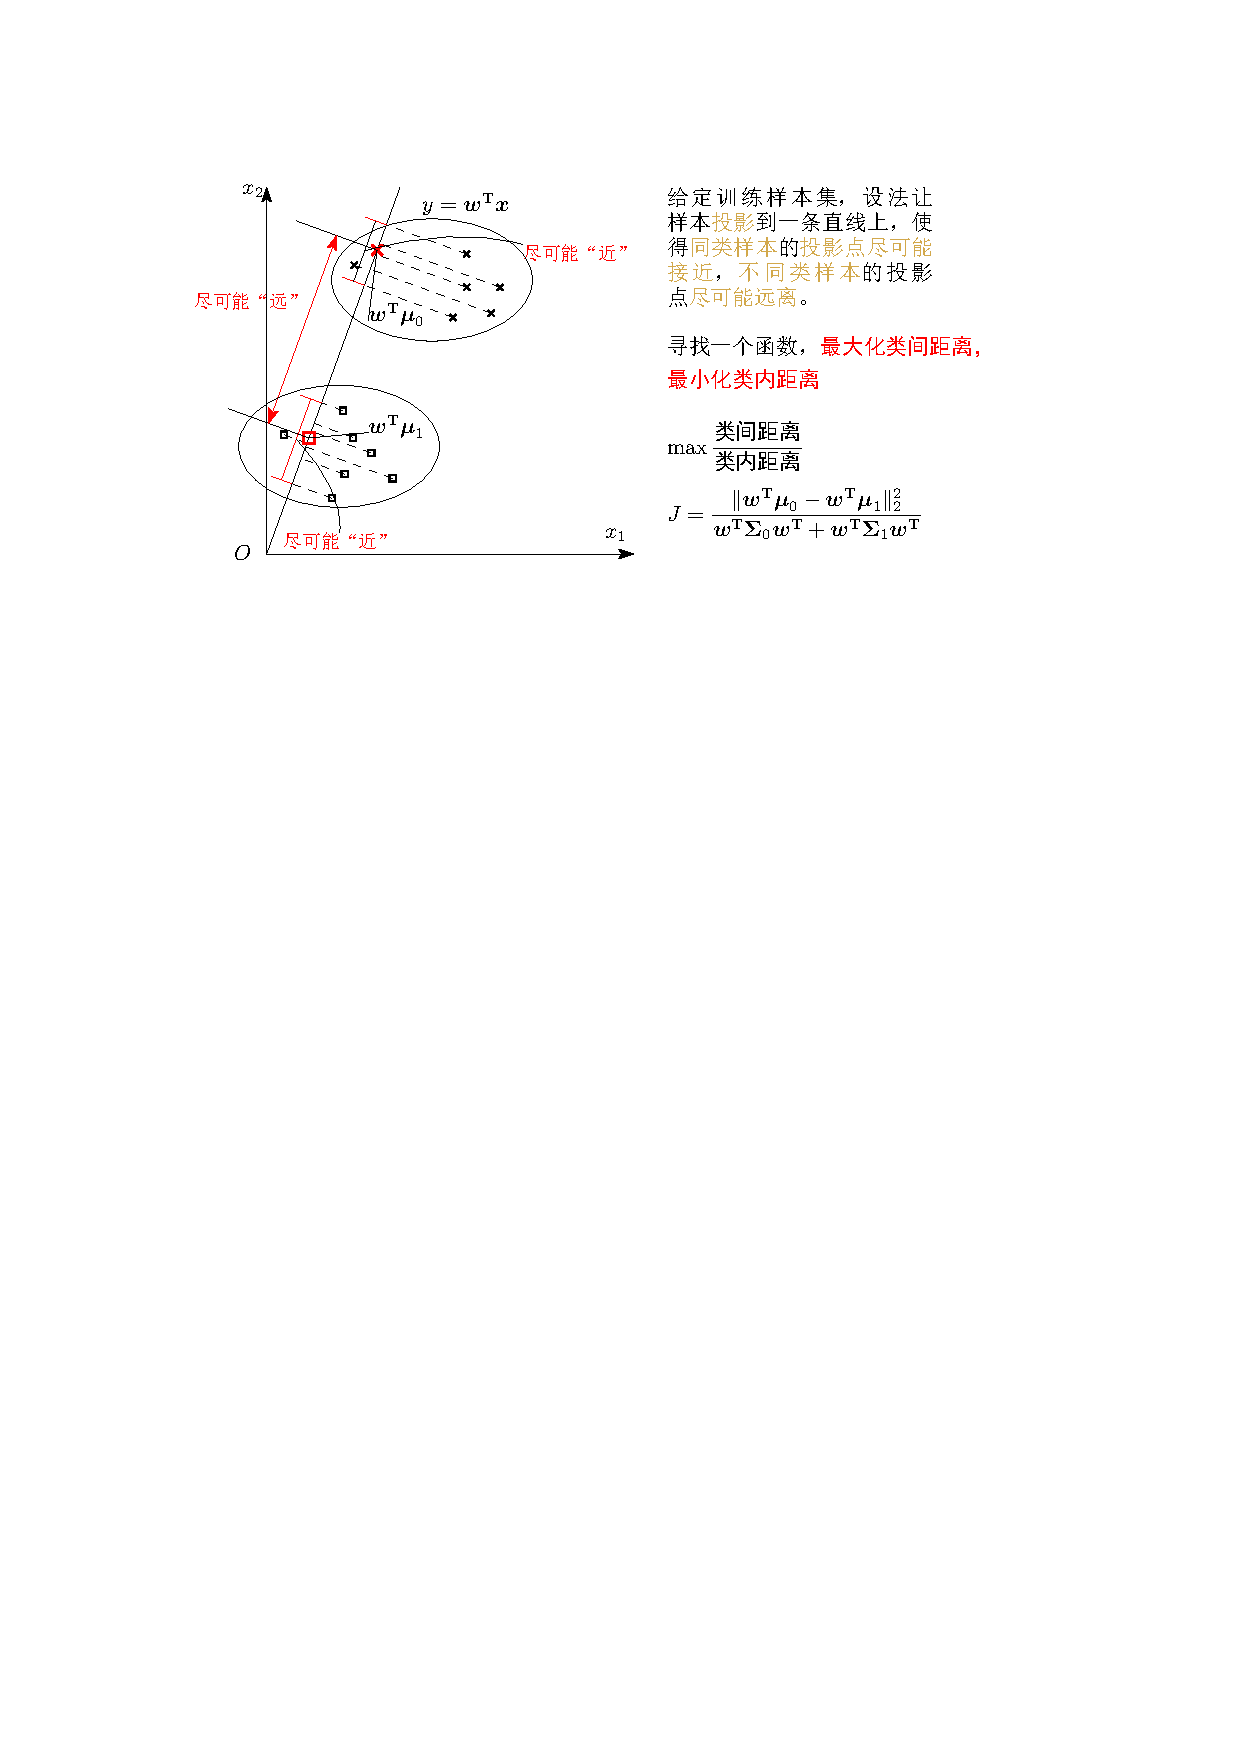
\includegraphics{image/线性判别分析.pdf}
\end{figure}
\[
    \begin{array}{ll}
        J &= \dfrac{\| \boldsymbol{w}^{\mathrm{T}}\boldsymbol{\mu}_0 - \boldsymbol{w}^{\mathrm{T}}\boldsymbol{\mu}_1 \|_2^2}{ \boldsymbol{w}^{\mathrm{T}}\boldsymbol{\Sigma}_0\boldsymbol{w}^{\mathrm{T}} + \boldsymbol{w}^{\mathrm{T}}\boldsymbol{\Sigma}_1\boldsymbol{w}^{\mathrm{T}} }\\
        &=\dfrac{\boldsymbol{w}^{\mathrm{T}}\left( \boldsymbol{\mu}_0-\boldsymbol{\mu}_1 \right)\left( \boldsymbol{\mu}_0-\boldsymbol{\mu}_1 \right)^{\mathrm{T}}\boldsymbol{w}}{ \boldsymbol{w}^{\mathrm{T}}\left( \boldsymbol{\Sigma}_0 + \boldsymbol{\Sigma}_1 \right)\boldsymbol{w}}
    \end{array}
\]
记$\boldsymbol{S}_{b} \overset{\triangle}{=}\left( \boldsymbol{\mu}_0-\boldsymbol{\mu}_1 \right)\left( \boldsymbol{\mu}_0-\boldsymbol{\mu}_1 \right)^{\mathrm{T}},\, \boldsymbol{S}_{w} \overset{\triangle}{=}\boldsymbol{\Sigma}_0 + \boldsymbol{\Sigma}_1$
那么
\[
    J = \dfrac{\boldsymbol{w}^{\mathrm{T}}\boldsymbol{S}_{b}\boldsymbol{w}}{ \boldsymbol{w}^{\mathrm{T}}\boldsymbol{S}_{w}\boldsymbol{w}}
\]
令$ \boldsymbol{w}^{\mathrm{T}}\boldsymbol{S}_{w}\boldsymbol{w} = 1$,最大化广义瑞利商等价形式为
\[
    \begin{array}{c}
        \min\limits_{\boldsymbol{w}} -\boldsymbol{w}^{\mathrm{T}}\boldsymbol{S}_{b}\boldsymbol{w}\\
        \operatorname{s.t.} \boldsymbol{w}^{\mathrm{T}}\boldsymbol{S}_{w}\boldsymbol{w} = 1
    \end{array}
\]
\textcolor{main1}{由拉格朗日乘子法可得}
\[
    \boldsymbol{S}_b\boldsymbol{w} = \lambda\boldsymbol{S}_{w}\boldsymbol{w}\rightarrow \boldsymbol{w} = \boldsymbol{S}_{w}^{-1}\left( \boldsymbol{\mu}_0-\mu_{1} \right)    
\]
两类数据同先验、满足高斯分布且协方差相等时,线性判别分析达到最优分类。
\begin{example}
    现有两类样本,请计算其线性判别分类器。
    \begin{itemize}
        \item 第1类:
        \[
            \boldsymbol{X}_1 = \left\{ (4,2),\,(2,4),\,(2,3),\,(3,6),\,(4,4) \right\}
        \]
        \item 第2类:
        \[
            \boldsymbol{X}_2 = \left\{ (9,10),\,(6,8),\,(9,5),\,(8,7),\,(10,8) \right\}
        \]
    \end{itemize}
    均值向量:
    \[
        \boldsymbol{\mu}_1 = \begin{bmatrix}
            3 & 3.8
        \end{bmatrix}^{\mathrm{T}},\,\boldsymbol{\mu}_2 = \begin{bmatrix}
            8.4 & 7.6
        \end{bmatrix}^{\mathrm{T}}
    \]
    散度矩阵:
    \[
        \boldsymbol{\Sigma}_1 = \begin{bmatrix}
            1   & -0.25 \\
            -0.25 & 2.2
        \end{bmatrix},\,\boldsymbol{\Sigma}_2 = \begin{bmatrix}
            2.3 & -0.05 \\
            -0.05 & 3.3
        \end{bmatrix}
    \]
    类内散度:
    \[
        \boldsymbol{S}_{w} = \boldsymbol{\Sigma}_1 + \boldsymbol{\Sigma}_2 = \begin{bmatrix}
            3.3 & -0.3 \\
            -0.3 & 5.5 \\
        \end{bmatrix}
    \]
    $\boldsymbol{S}_{w}$的逆
    \[
        \boldsymbol{S}_{w}^{-1} = \begin{bmatrix}
            0.30454 & 0.016611 \\
            0.016611 & 0.182724 \\
        \end{bmatrix}
    \]
    故而$\boldsymbol{w}$为
    \[
        \boldsymbol{w} = \boldsymbol{S}_{w}^{-1}\left( \boldsymbol{\mu}_0-\boldsymbol{\mu}_1 \right) = \begin{bmatrix}   
            -1.70764 & -0.78405
        \end{bmatrix}^{\mathrm{T}}
    \]
\end{example}

\textcolor{main1}{支持向量机}

\begin{figure}[htbp]
    \centering
    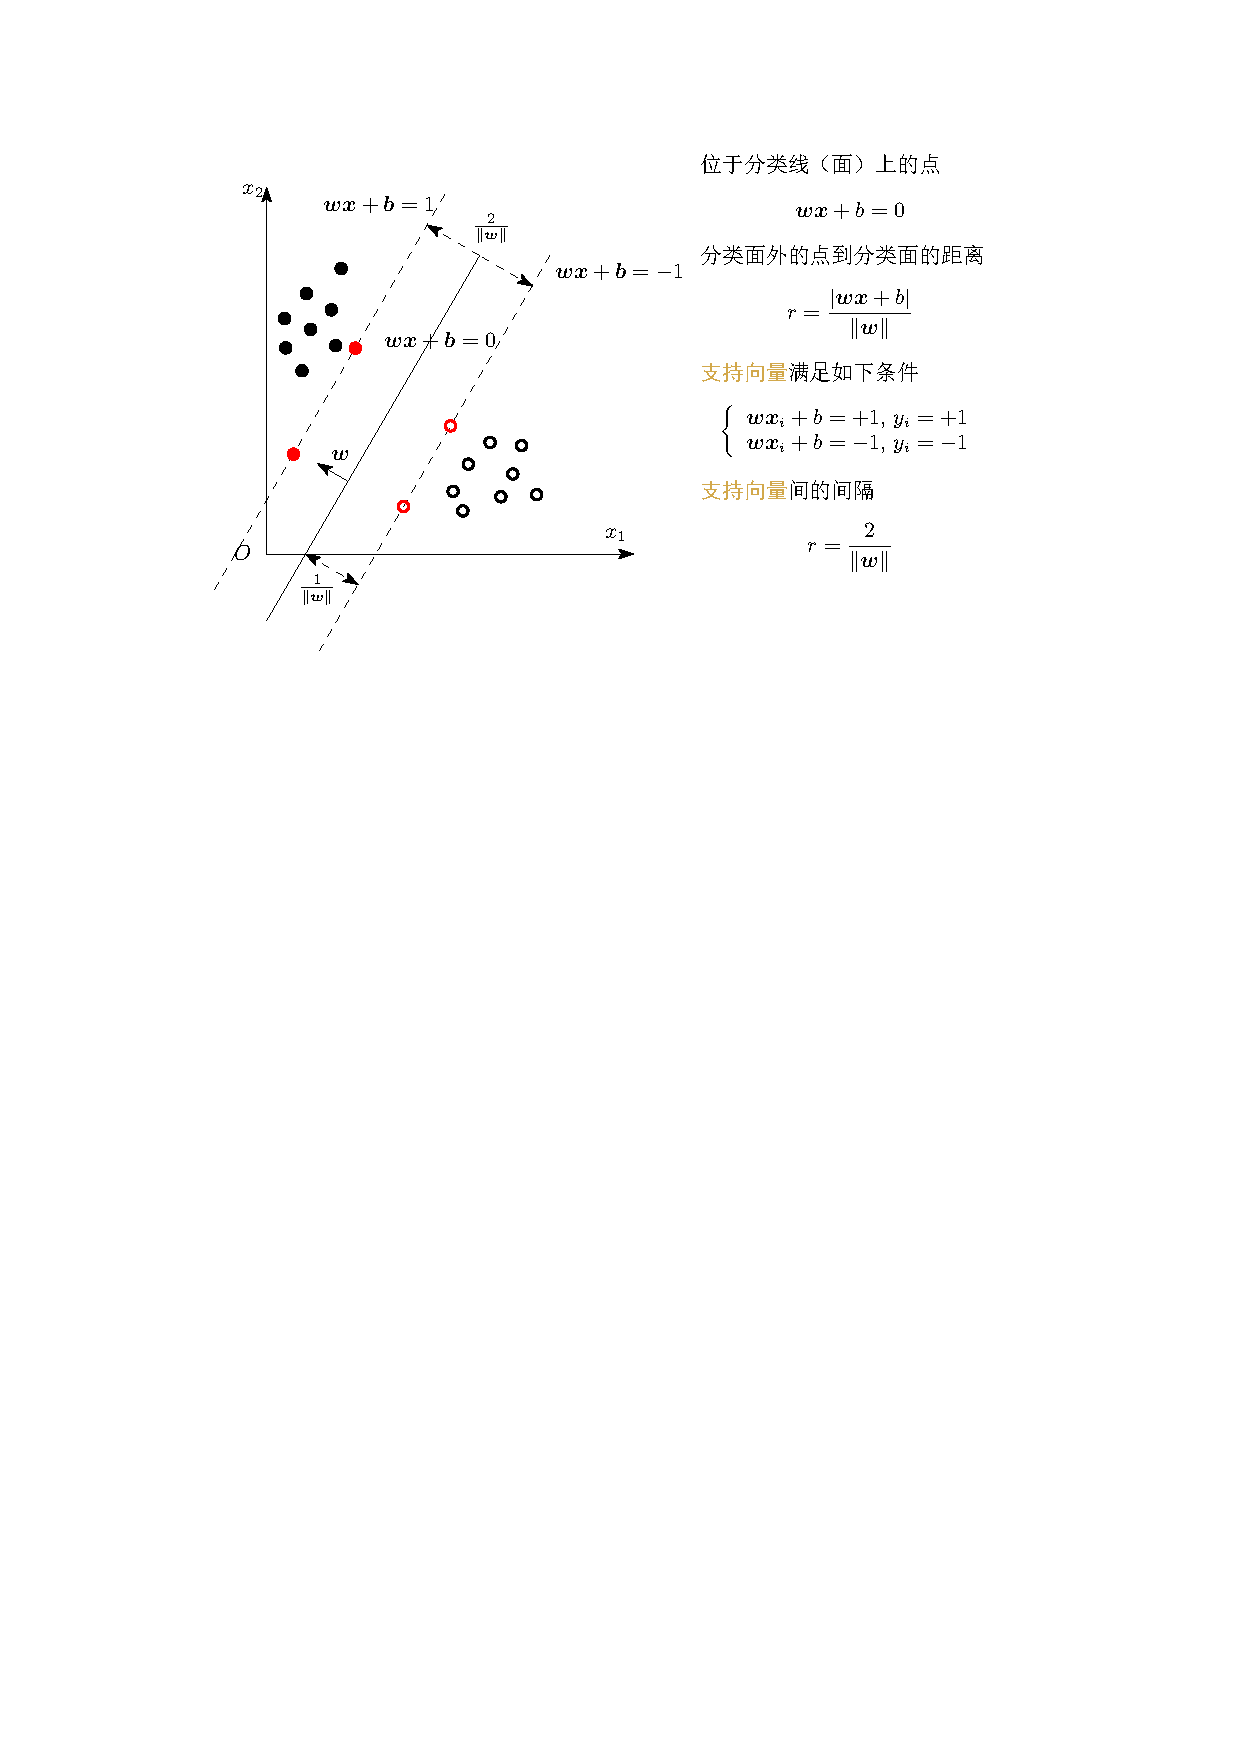
\includegraphics{image/支持向量机.pdf}
\end{figure}
\textcolor{main1}{最大间隔原则:}

选择参数对$(\boldsymbol{w},b)$使得训练集对于线性函数$\boldsymbol{wx}+b = 0$的几何间隔取最大值,构造决策函数
\[
    \begin{array}{l}
        \min\limits_{\boldsymbol{w},b} \dfrac{1}{2}\|\boldsymbol{w}\|^2\\
        \operatorname{s.t.}\, y_i\left( \boldsymbol{wx}_i+b \right)\geq 1
    \end{array}
\]
为求解上述问题,使用使用Lagrange乘子法将其转化为对偶问题。于是引入Lagrange函数:
\[
    L\left( \boldsymbol{w},b,\alpha \right) = \dfrac{1}{2}\|\boldsymbol{w}\|^2 - \sum\limits_{i = 1}^{n}\alpha_i\left( y_i\left( \boldsymbol{wx}_i+b \right)-1 \right)
\]
首先求Lagrange函数关于$\boldsymbol{w},\,b$的极小值。由极值条件有:
\[
    \nabla_{b}L\left( \boldsymbol{w},b,\alpha \right) = 0,\,\nabla_{w}L\left( \boldsymbol{w},b,\alpha \right) = 0
\]
得到
\[
    \sum\limits_{i = 1}^{n}y_{i}\alpha_i = 0,\,\boldsymbol{w} = \sum\limits_{i = 1}^{n}y_{i}\alpha_i\boldsymbol{x}_i
\]

\begin{example}
    现有三个样本能被支持向量机正确分类且远离决策超平面。如果把这三个样本加入到训练集,支持向量机的决策超平面是否会受其影响?为什么?
    \begin{enumerate}[A]
        \item 会
        \item \textcolor{main1}{不会}
    \end{enumerate}
\end{example}
\textcolor{main1}{K 近邻}
\begin{figure}[htbp]
    \centering
    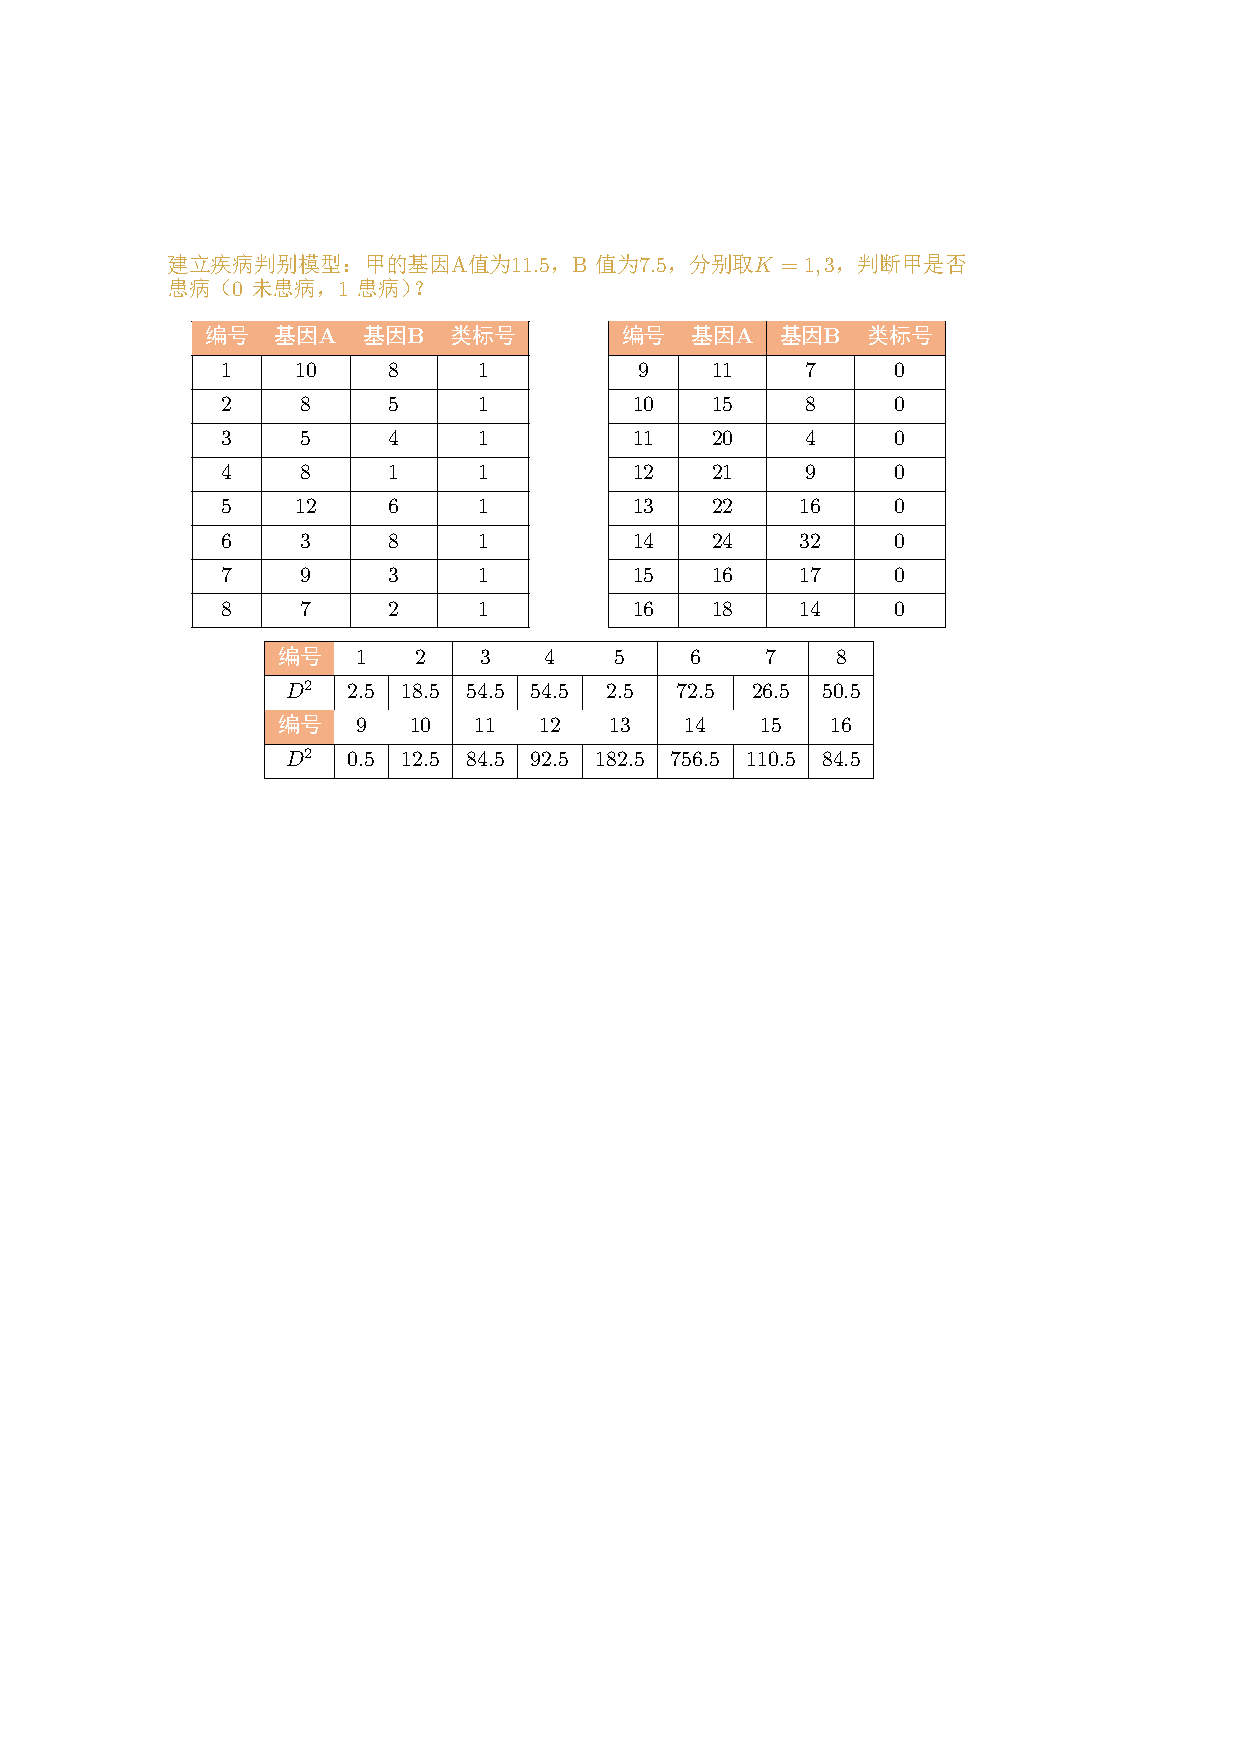
\includegraphics[scale = 0.95]{image/K近邻.pdf}
\end{figure}
\begin{itemize}
    \item $K = 1$,未患病。
    \item $K = 3$,患病。
\end{itemize}
\textcolor{main1}{K近邻法的优点}
\begin{itemize}
    \item 简单,易于理解,易于实现,无需参数估计,无需训练;
    \item 对异常值不敏感,个别噪音数据对结果的影响不是很大;
    \item 适合对稀有事件进行分类;
    \item 适合于多分类问题,K 近邻要比支持向量机表现要好。
\end{itemize}
\textcolor{main1}{K近邻法的缺点}
\begin{itemize}
    \item 对测试样本分类时的计算量大,内存开销大,需要计算新样本到全体已知样本的距离,才能求得它的K 个最近邻点;
    \item 当样本不平衡时,可能导致新样本的K 个邻居中大容量类的样本占多数,出现系统分类偏差;
    \item K近邻是一种消极学习方法、懒惰算法。
\end{itemize}

\textcolor{main1}{决策树}

\begin{note}
    决策树学习的关键是:选择最优划分属性
    \begin{itemize}
        \item 什么样的划分属性是最优的?
        
        希望决策树的分支结点所包含的样本尽可能属于同一类别,即结点的“纯度”越来越高,可以高效地从根结点到达叶结点,得到决策结果。
        \item 三种度量结点“纯度”的指标
        \begin{itemize}
            \item 信息增益:ID3
            \item 增益率:C4.5
            \item 基尼指数:CART
        \end{itemize}
    \end{itemize}
\end{note}
\begin{note}
    决策树的优缺点:
    \begin{itemize}
        \item 优点
        \begin{itemize}
            \item 计算复杂度不高;
            \item 可解释性强;
            \item 能处理具有许多属性的数据集;
            \item 在相对短的时间内能够对大数据集做出可行且效果良好的分类结果。
        \end{itemize} 
        \item 缺点
        \begin{itemize}
            \item 可能存在过拟合问题
        \end{itemize} 
    \end{itemize}
\end{note}

\begin{note}
    剪枝是解决决策树过拟合的一种方法:——通过主动去掉一些分支来降低过拟合的风险

    \begin{itemize}
        \item 预剪枝:
        
        在决策树生成过程中,对每个结点在划分前先进行估计,若当前结点的划分不能带来决策树泛化性能提升,则停止划分并将当前结点标记为叶结点。
        \item 后剪枝:
        
        先从训练集生成一棵完整的决策树,然后自底向上地对非叶结点进行考察,若将该结点对应的子树替换为叶结点能带来决策树泛化性能提升,则将该子树替换为叶结点。
    \end{itemize}
\end{note}

\begin{note}
    在医疗诊断等应用场景中,\textcolor{main1}{灵敏度、特异度、阳性预测值、阴性预测值}等比单纯的错误率 准确率更重要。
    \begin{figure}[htbp]
        \centering
        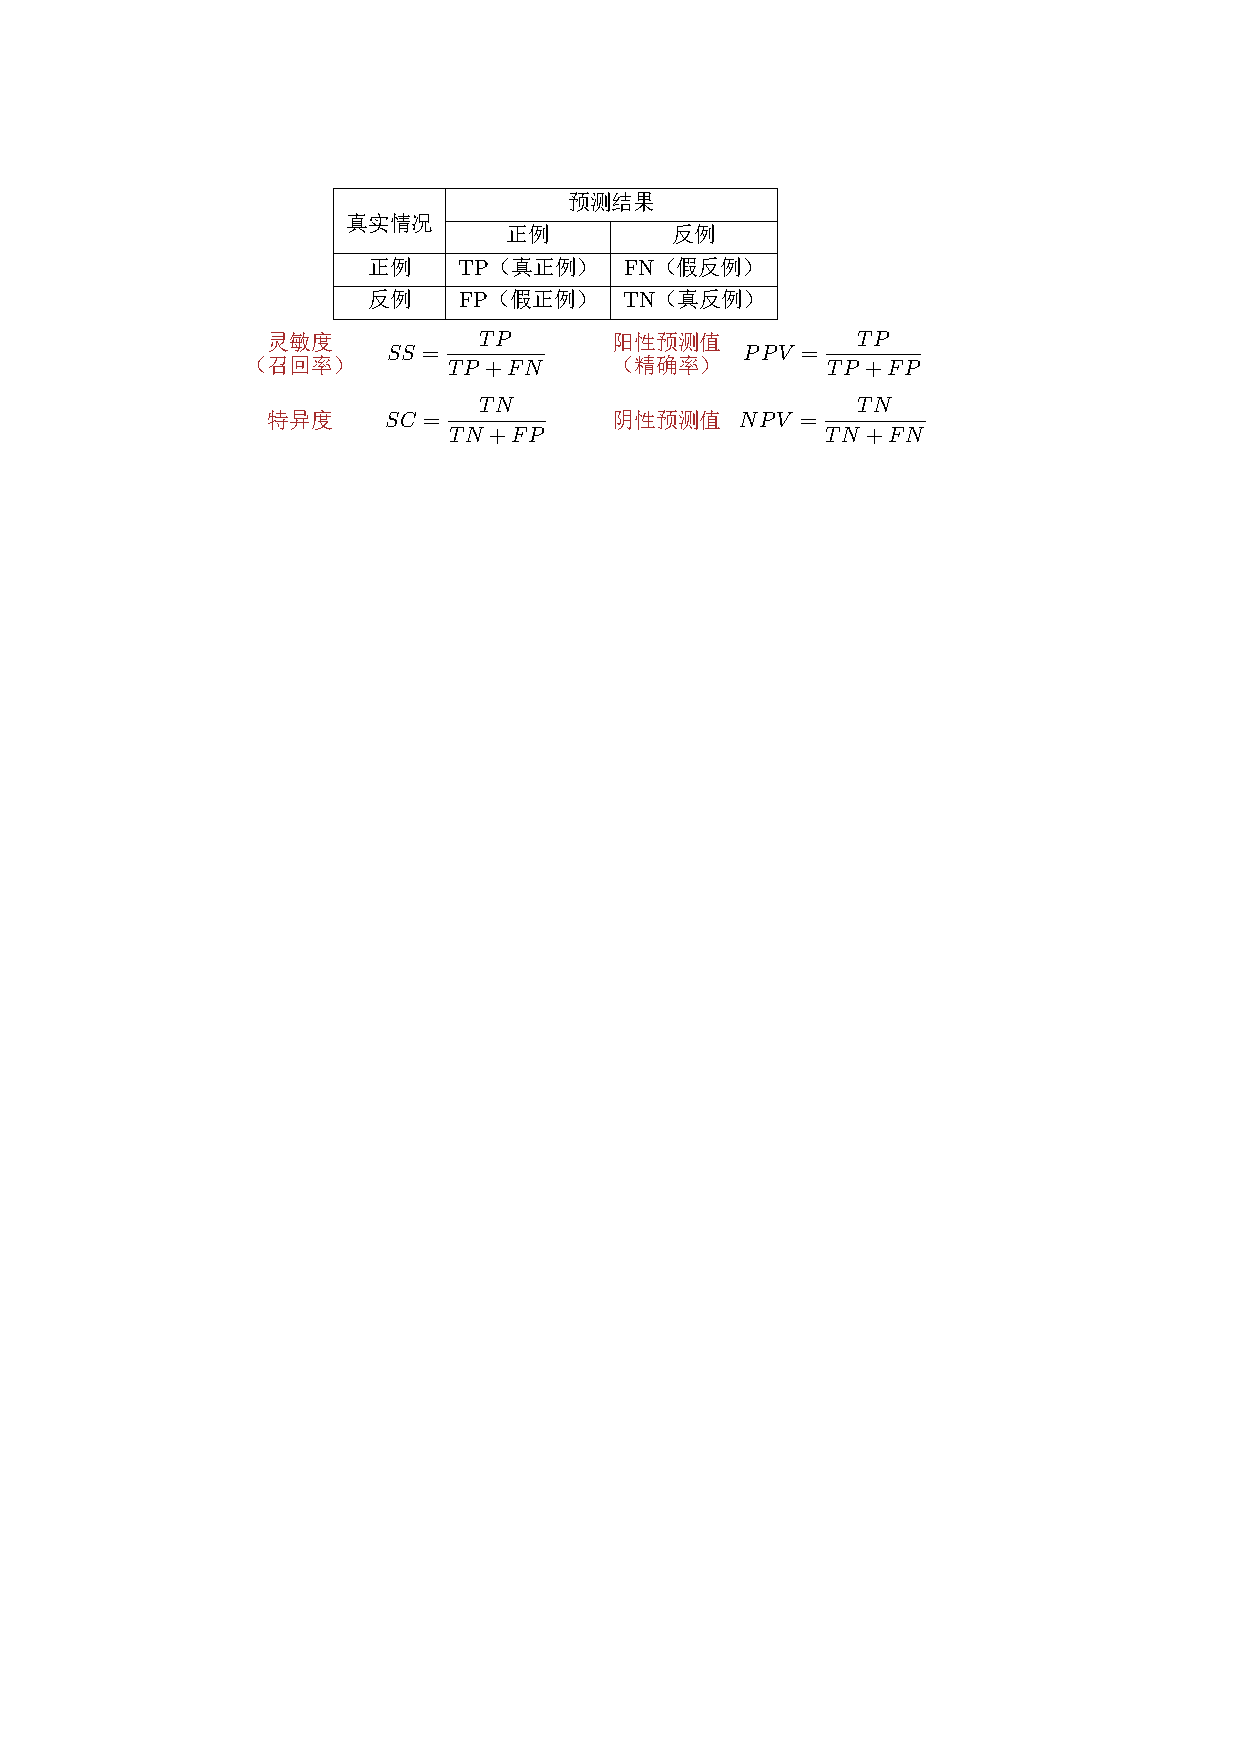
\includegraphics{image/决策树.pdf}
    \end{figure}
\end{note}
\begin{example}
    已知某核酸检测分类器对COVID 19 阳性和阴性样本预测的混淆矩阵如下表所示,该分类方法的灵敏度为\textcolor{main1}{[$\dfrac{3}{3+7} = 30\%$]} 、特异度为\textcolor{main1}{[$\dfrac{9}{1+9} = 90\%$]} 、准确率为\textcolor{main1}{[$\dfrac{3+9}{20} = 30\%$]}。
    \begin{figure}[htbp]
        \centering
        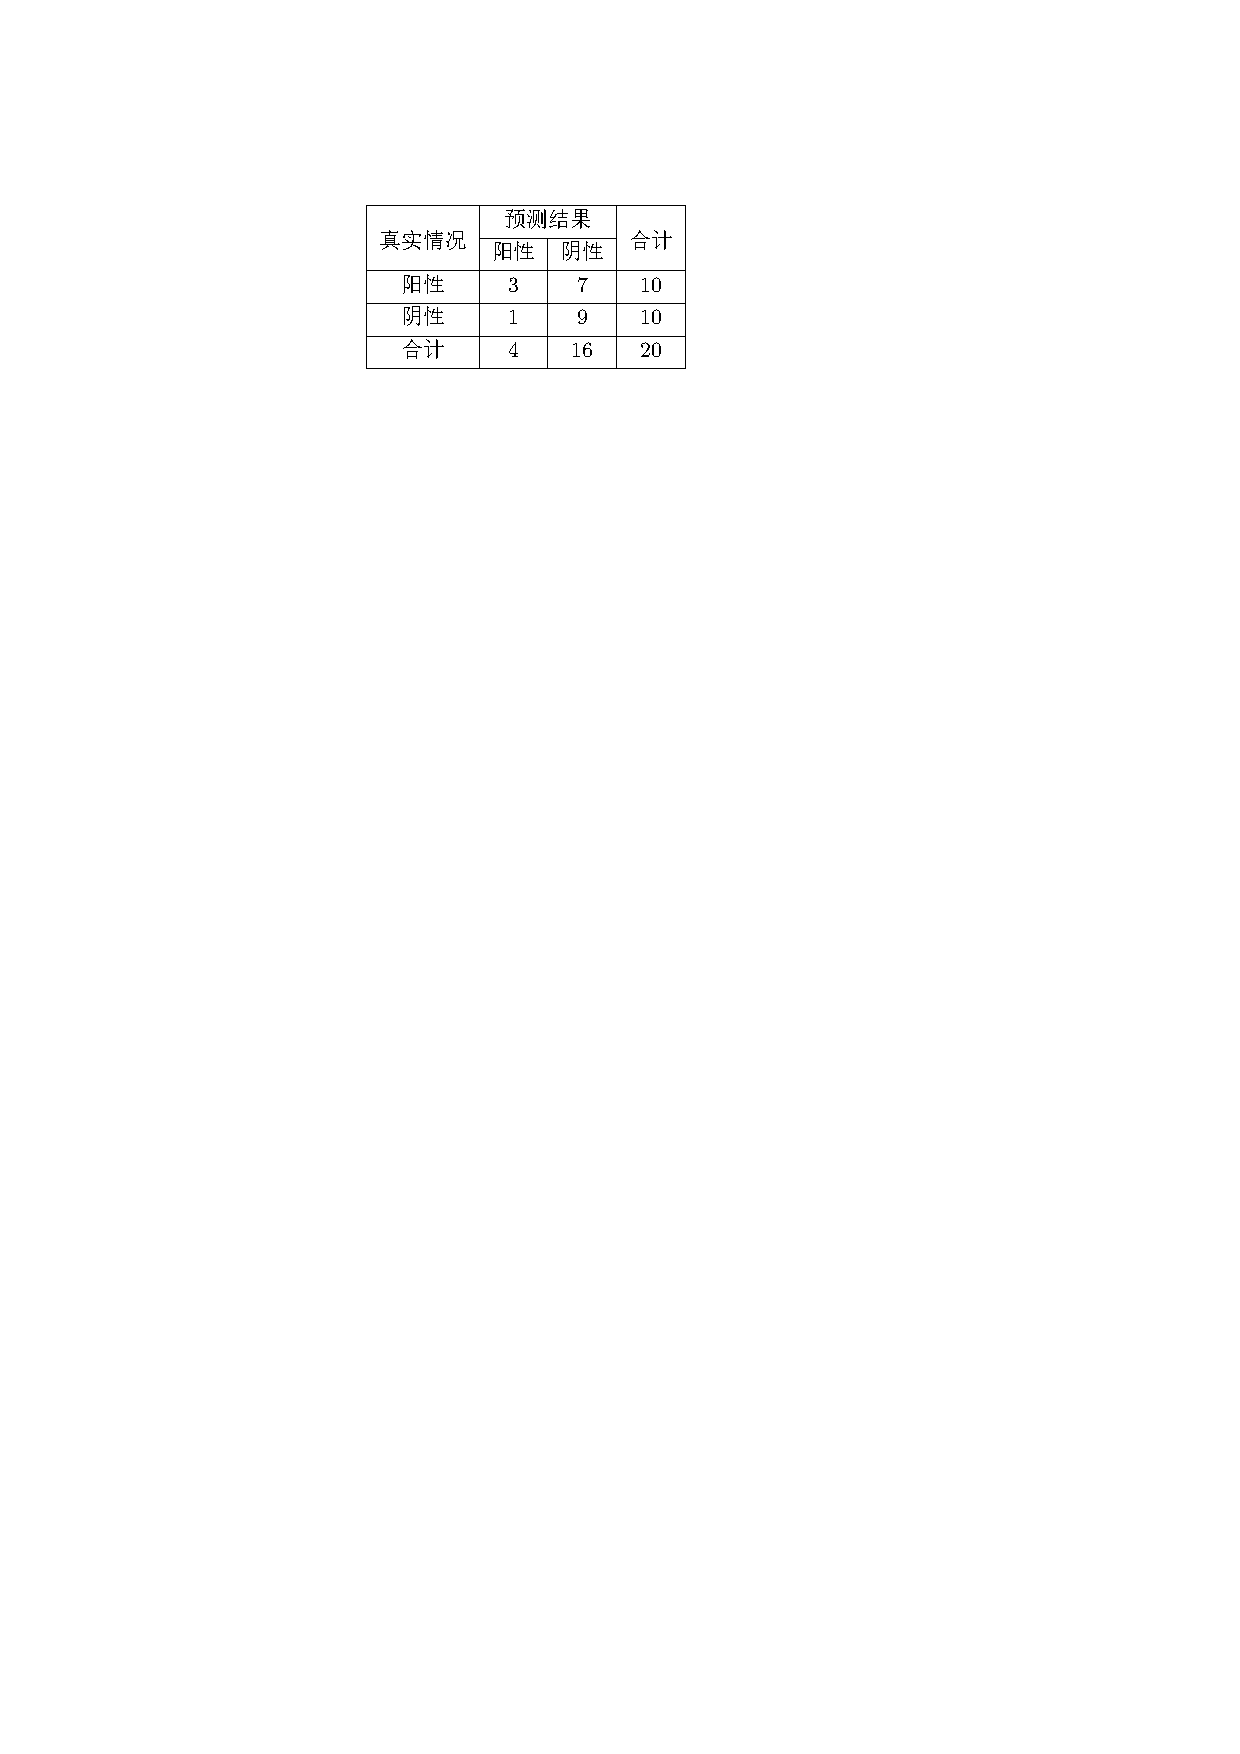
\includegraphics{image/混淆矩阵例题.pdf}
    \end{figure}
\end{example}
\subsection{无监督学习基本方法}
\textcolor{main1}{无监督学习(聚类)的一般过程}
\begin{definition}[无监督学习]
    根据数据的相似性将数据分为多类的过程。
\end{definition}
\textcolor{main1}{目标}:将数据集中的样本按照相似性划分为若干个通常不相交的子集“簇”。
\begin{figure}[htbp]
    \centering
    \includegraphics{image/聚类目标.pdf}
\end{figure}
\subsubsection{相似性的度量}
\textcolor{main1}{闵可夫斯基距离}

\begin{definition}[闵可夫斯基距离]
    设$\boldsymbol{x}_{i} = \left( x_{i1},\cdots,_{ip} \right)$和$\boldsymbol{x}_{j} = \left( x_{j1},\cdots,_{jp} \right)$是$i$和$j$哥样本的特征向量,则二者之间的距离为
    \[
        d_{ij} = \left( \sum\limits_{k = 1}^{p}|x_{ik}-x_{jk}|^{g} \right)^{1/g}
    \]
    \begin{itemize}
        \item 当$g = 1$时(绝对值距离),$d_{ij} = \sum\limits_{k = 1}^{p}|x_{ik}-x_{jk}|$
        \item 当$g = 2$时(欧式距离),$d_{ij} = \sqrt{\sum\limits_{k = 1}^{p}\left( x_{ik}-x_{jk} \right)^2}$
    \end{itemize}
\end{definition}
\begin{note}
    闵式距离的缺陷
    \begin{itemize}
        \item 容易受变量的量纲影响
        \item 没有考虑变量间的相关性
    \end{itemize}
\end{note}
\begin{note}
    两种改进措施
    \begin{itemize}
        \item $\text{变量标准化处理}\left\{ \begin{array}{ll}
            \text{极差标准化} & y_i = \dfrac{x_{i}-\min x}{\max x-\min x} \\
            \text{Z-score标准化} & z_i = \dfrac{x_i-\operatorname{mean}(x)}{\sigma}
        \end{array} \right.$
        \item 马氏距离 $ D_{M}(x) = \sqrt{\left( \boldsymbol{x}-\boldsymbol{\mu} \right)^{\mathrm{T}}\boldsymbol{S}^{-1}\left( \boldsymbol{x}-\boldsymbol{\mu} \right)}$
    \end{itemize}
\end{note}
\textcolor{main1}{方向余弦度量相似度}
\begin{definition}[方向余弦]
    $n$维向量$x$和$y$的夹角记作$\theta$,根据余弦定理,其余弦值为
    \[
        \cos (\theta) = \dfrac{\boldsymbol{x}^{\mathrm{T}}\boldsymbol{y}}{|\boldsymbol{x}||\boldsymbol{y}|} = \dfrac{\sum\limits_{k = 1}^{p}x_{ik}x_{jk}}{\sqrt{\sum\limits_{k = 1}^{p}x_{ik}^2 \sum\limits_{k = 1}^{p}x_{jk}^2}}
    \]
\end{definition}

\textcolor{main1}{相关系数}
\begin{definition}[相关系数]
    设$\boldsymbol{x}_{i} = \left( x_{i1},\cdots,_{ip} \right)$和$\boldsymbol{x}_{j} = \left( x_{j1},\cdots,_{jp} \right)$是$i$和$j$哥样本的特征向量,则二者之间的相关系数为
    \[
        r_{ij} = \dfrac{\sum\limits_{k = 1}^{p}\left( x_{ik}-\bar{x_{i}} \right)\left( x_{jk}-\bar{x_{j}} \right)}{\sqrt{\left[\sum\limits_{k = 1}^{p} \left( x_{ik}-\bar{x_{i}} \right)^2 \right]\left[\sum\limits_{k = 1}^{p} \left( x_{jk}-\bar{x_{j}} \right)^2 \right]}}
    \]
\end{definition}
\begin{note}
    相关系数和方向余弦关系
    \begin{figure}[htbp]
        \centering
        \includegraphics{image/余弦和相关系数关系.pdf}
    \end{figure}
\end{note}
\begin{note}
    常用聚类方法:
    \begin{itemize}
        \item 划分法:\textcolor{main1}{需要输入类别数},适用于\textcolor{main2}{样本数较多}的情况
        \item 层次法:\textcolor{main1}{不需要输入类别数},适用于\textcolor{main2}{样本数较少}的情况
    \end{itemize}
\end{note}
\subsubsection{划分法}
\begin{definition}[划分法]
    给定一个有$N $个样本的数据集,划分法将构造$K $个分组,每一个分组就代表一个聚类,$K<N$ 。而且这$K $个聚类满足两个条件:
    \begin{itemize}
        \item 每一个聚类至少包含一个样本;
        \item 每一个样本属于且仅属于一个聚类。
    \end{itemize}

    \textcolor{main1}{标准:}同一聚类中的样本相似性高,不同聚类中的样本相似性低

    \textcolor{main1}{典型算法:}K 均值聚类算法、K MEDOIDS 算法、CLARANS 算法
\end{definition}

\textcolor{main1}{K均值聚类}
\begin{note}
    基本思想
    
    将每一个样本分配到最近中心(样本均值)所属的簇

    \textcolor{main1}{目标函数:}$C^{*} = \arg\min\limits_{C}\sum\limits_{l = 1}^{K}\sum\limits_{C(i) = l}\|\boldsymbol{x}_i-\bar{\boldsymbol{x}_l}\|^2$

    \textcolor{main1}{优化方法:}采用贪心策略,通过迭代优化来近似求解,不能保证收敛到全局最优

    算法主要包括以下步骤:
    \begin{enumerate}
        \item 指定聚类数,确定初始簇的中心
        
        用户指定或系统指定。
        \item 根据距离最近原则进行分类
        
        计算每个样本到各簇中心点的距离, 并按距离最近原则对所有样本进行分类,计算新的聚类中心。
        \item 迭代,直至收敛
    \end{enumerate}
\end{note}
\begin{example}
    对A 、B 、C 、D 样本分别测量特征$X_1$ 和$X_2$,得到如下结果。
    \begin{figure}[htbp]
        \centering
        \includegraphics{image/K均值.pdf}
    \end{figure}
    试用K 均值方法将这四个样本聚成两簇。
    \begin{enumerate}
        \item 按要求取$K = 2$,将样本随意分成两簇(A,B)和(C,D),计算两个聚类的中心坐标。计算样本到各簇中心的欧氏距离,将样本分配给最近的一簇。对于样本有变动的簇,重新计算它们的中心坐标。
        % Table generated by Excel2LaTeX from sheet 'K均值'
        \begin{table}[htbp]
            \centering
            \begin{tabular}{|c|c|c|c|c|c|c|}
            \hline
            \multirow{2}[4]{*}{聚类} & \multicolumn{2}{c|}{中心坐标} & \multicolumn{4}{c|}{$D^2(i,C_l)$} \bigstrut\\
        \cline{2-7}        & $X_1$ & $X_2$ & A   & B   & C   & D \bigstrut\\
            \hline
            $(A,B)$ & 2   & 2   & 10  & 10  & 17  & 41 \bigstrut\\
            \hline
            $(C,D)$ & -1  & -2  & 61  & 9   & 4   & 4 \bigstrut\\
            \hline
            \end{tabular}%
        \end{table}%

        B被分配到$(C,D)$
        \item 再次检查每个样本,以决定是否需要重新分簇。计算样本到各中心的距离。
        % Table generated by Excel2LaTeX from sheet 'K均值'
        \begin{table}[htbp]
            \centering
            \begin{tabular}{|c|c|c|c|c|c|c|}
            \hline
            \multirow{2}[4]{*}{聚类} & \multicolumn{2}{c|}{中心坐标} & \multicolumn{4}{c|}{$D^2(i,C_l)$} \bigstrut\\
        \cline{2-7}        & $X_1$ & $X_2$ & A   & B   & C   & D \bigstrut\\
            \hline
            $(A)$ & 5   & 3   & 0   & 40  & 41  & 89 \bigstrut\\
            \hline
            $(B,C,D)$ & -1  & -1  & 52  & 4   & 5   & 5 \bigstrut\\
            \hline
            \end{tabular}%
        \end{table}%
        
        由于每个样本都已经分配到距离中心最近的簇,因此聚类过程到此结束。最终得到$K=2 $的聚类结果是$A $独自成一簇,$B,\,C,\,D $聚成一簇。
    \end{enumerate}
\end{example}
\begin{example}
    请判断以下说法是否正确:当距离度量和聚类数目选定后,$K $均值聚类的结果是唯一的。
    \begin{enumerate}[A]
        \item 正确
        \item \textcolor{main1}{错误}
    \end{enumerate}
\end{example}
\begin{note}
    $K $均值聚类:优缺点
    \begin{itemize}
        \item 优点
        \begin{itemize}
            \item 简单快速,可以用于多种数据类型
            \item 有效,可处理大数据集
        \end{itemize}
        \item 缺点
        \begin{itemize}
            \item 结果受初始聚类中心影响较大
            \item 不适合处理非球形簇、不同尺度和不同密度的簇
            \item 结果受聚类数影响较大
            \item 对噪声和孤立点数据敏感
        \end{itemize}
    \end{itemize}
\end{note}
\begin{note}
    均值聚类的改进
    \begin{itemize}
        \item 初始聚类中心的选择
        \begin{itemize}
            \item 选择彼此距离尽可能远的$K $个点
            \item 选择密度最大的$K $个点
        \end{itemize}
        \item 聚类数的选择
        \begin{itemize}
            \item 观察法
            \item 肘部法
            \begin{itemize}
                \item 随着聚类数$K $增大,样本划分更加精细,每个簇的聚合程度逐渐提高,误差平方和变小;
                \item 当$K $小于真实聚类数时, $K $增大会大幅增加每个簇的聚合程度,误差平方和的下降幅度很大;
                \item 当$K $到达真实聚类数时,误差平方和的下降幅度骤减,然后随着$K $值的继续增大而趋于平缓;
                \item 误差平方和与$K $的关系图是一个手肘的形状,而肘部对应的$K $ 值就是数据的真实聚类数。
            \end{itemize}
        \end{itemize}
        \item 离群点的处理
        \begin{itemize}
            \item 离群点检测和删除
        \end{itemize}
    \end{itemize}
\end{note}
\subsubsection{层次法}
\begin{definition}[层次聚类方法]
    通过计算数据集中样本间的相似性来创建一棵有层次的嵌套聚类树。
\end{definition}

\textcolor{main1}{创建聚类树的策略}
\begin{figure}[htbp]
    \centering
    \includegraphics{image/创建聚类树的策略.pdf}
\end{figure}

\textcolor{main1}{自底向上的层次聚类过程}
\begin{figure}[htbp]
    \centering
    \includegraphics{image/自底向上.pdf}
\end{figure}
\begin{note}
    三个要素:距离度量、合并规则和结束条件
\end{note}
\begin{note}
    思考:

    给定两两样本之间的距离度量函数,对于由两个或者多个样本合并之后得到的新簇,要如何确定它们与其他簇之间的距离呢?
\end{note}
\begin{note}
    \textcolor{main1}{簇间的距离}

    给定据类簇$C_i$和$C_j$
    \begin{itemize}
        \item \textcolor{main1}{最小距离:}$ d_{\min}\left( C_i,C_j \right) = \min\limits_{\boldsymbol{x}\in C_{i},\boldsymbol{z}\in C_{j}} \operatorname{dist}\left( \boldsymbol{x},\boldsymbol{z} \right) $
        \item \textcolor{main1}{最大距离:}$ d_{\max}\left( C_i,C_j \right) = \max\limits_{\boldsymbol{x}\in C_{i},\boldsymbol{z}\in C_{j}} \operatorname{dist}\left( \boldsymbol{x},\boldsymbol{z} \right) $
        \item \textcolor{main1}{平均距离:}$ d_{\operatorname{avg}}\left( C_i,C_j \right) = \dfrac{1}{|C_i||C_j|}\sum\limits_{\boldsymbol{x}\in C_{i}}\sum\limits_{\boldsymbol{z}\in C_{j}} \operatorname{dist}\left( \boldsymbol{x},\boldsymbol{z} \right) $
    \end{itemize}

    \textcolor{main1}{最小距离}由两个簇的\textcolor{main1}{最近样本}决定,\textcolor{main1}{最大距离}由两个簇的\textcolor{main1}{最远样本}决定,而\textcolor{main1}{平均距离}由两个簇的\textcolor{main1}{所有样本}共同决定。
\end{note}

\begin{example}
    层次聚类的结果是不是唯一的?
    \begin{enumerate}[A]
        \item 唯一
        \item \textcolor{main1}{不唯一}
    \end{enumerate}
\end{example}
\begin{example}
    设有6个样本,对每个样本测量一个特征,分别是1、2、5、7、9、10,用基于\textcolor{main1}{最小距离}的层次法将它们分类。
    \begin{figure}[htbp]
        \centering
        \includegraphics{image/层次聚类举例.pdf}
    \end{figure}
    \begin{enumerate}
        \item 选择绝对距离作为距离度量,形成距离矩阵$D_{(0)}$
        % Table generated by Excel2LaTeX from sheet '层次聚类'
        \begin{table}[htbp]
            \centering
            \begin{tabular}{c|cccccc}
            \hline
                & $G_1$ & $G_2$ & $G_3$ & $G_4$ & $G_5$ & $G_6$ \\
                \hline
            $G_1$ & 0   &     &     &     &     &  \\
            $G_2$ & 1   & 0   &     &     &     &  \\
            $G_3$ & 4   & 3   & 0   &     &     &  \\
            $G_4$ & 6   & 5   & 2   & 0   &     &  \\
            $G_5$ & 8   & 7   & 4   & 2   & 0   &  \\
            $G_6$ & 9   & 8   & 5   & 3   & 1   & 0 \\
            \hline
            \end{tabular}%
        \end{table}%
        \item 矩阵$D_{(0)}$中最小元素是$D_{12}=D_{56} = 1$,将$G_1$和$G_2$合并为$G_7$,$G_5$和$G_6$合并为$G_8$,并计算新簇与其他簇的距离$D_{(1)}$
        % Table generated by Excel2LaTeX from sheet '层次聚类'
        \begin{table}[htbp]
            \centering
            \begin{tabular}{c|cccc}
            \hline
                & $G_7$ & $G_3$ & $G_4$ & $G_8$ \bigstrut\\
            \hline
            $G_7$ & 0   &     &     &  \bigstrut[t]\\
            $G_3$ & 3   & 0   &     &  \\
            $G_4$ & 5   & 2   & 0   &  \\
            $G_8$ & 7   & 4   & 2   & 0 \bigstrut[b]\\
            \hline
            \end{tabular}%
        \end{table}%
        \item 距离矩阵$D_{(1)}$中最小值是$D_{34} = D_{48} = 2$,将$G_4$与$G_3$合并,再与$G_8$合并,因此$G_3,\,G_4,\,G_8$合并成为一个新簇$G_9$,计算它与其他簇的距离$D_{(2)}$
        % Table generated by Excel2LaTeX from sheet '层次聚类'
        \begin{table}[htbp]
            \centering
            \begin{tabular}{c|cc}
            \hline
                & $G_7$ & $G_9$ \bigstrut\\
            \hline
            $G_7$ & 0   &  \bigstrut[t]\\
            $G_9$ & 3   & 0 \bigstrut[b]\\
            \hline
            \end{tabular}%
        \end{table}%
        \item 最后将$G_7$和$G_9$合并成$G_{10}$,这时所有的样本聚为一类,聚类过程结束
        \begin{figure}
            \centering
            \includegraphics{image/层次聚类举例可视化.pdf}
        \end{figure}
    \end{enumerate}
\end{example}
\begin{note}
    层次聚类的优缺点:
    \begin{itemize}
        \item 优点
        \begin{itemize}
            \item 不需要预先设定聚类数
            \item 可以发现簇的层次关系
            \item 可以聚类成除球形簇之外的其它形状
        \end{itemize}
        \item 缺点
        \begin{itemize}
            \item 计算复杂度高
            \item 对离群点敏感
            \item 可能聚成链状
        \end{itemize}
    \end{itemize}
\end{note}
\subsection{人工神经网络}
\subsubsection{生物神经元与神经网络}
神经元是神经系统结构与功能的基本单元。
\begin{figure}[htbp]
    \centering
    \includegraphics[width = .5\textwidth]{image/NeuronFreeVectorIllustration.pdf}
\end{figure}
\begin{itemize}
    \item 树突:神经纤维接收器,将电信号传送到细胞体
    \item 细胞体:对输入信号进行整合和阈值处理
    \item 轴突:把细胞体的输出信号导向其他神经元
    \item 突触:一个神经细胞的轴突和另一个神经细胞树突的结合点
\end{itemize}
\begin{note}
    生物神经元的信息处理过程:
    \begin{itemize}
        \item 信息输入
        \item 空间整合:同一时刻产生的刺激所引起的膜电位变化,大致等于各单独刺激引起的膜电位变化的代数和。
        \item 时间整合:各输入脉冲抵达神经元的时间先后不一样。总的突触后膜电位为一段时间内的累积。
        \item 信息产生
        \item 信息传导
        \item 兴奋或抑制
    \end{itemize}
    小结:树突从细胞体伸向其它神经元,神经元之间通过突触连接。通过突触输入的信号起着兴奋 抑制作用。当细胞体接受的累加兴奋作用超过某阈值时,细胞进入兴奋状态,产生冲动,并由轴突输出。
\end{note}
\begin{note}
    生物神经元的基本特点:
    \begin{itemize}
        \item 神经元传递信息过程为多输入、单输出;
        \item 输入信号可以起兴奋作用,也可以起抑制作用;
        \item 神经元之间的连接强度可以随训练而改变,并决定信号传递的强弱;
        \item 每个神经元有一个“阈值”,一个神经元接受信号的累积效果决定该神经元的状态。
    \end{itemize}
\end{note}
\begin{example}
    生物神经元基本特点不包括:    
    \begin{enumerate}[A]
        \item 多输入单输出
        \item 时空整合功能
        \item \textcolor{main1}{兴奋性}
        \item 阈值特性
    \end{enumerate}
\end{example}
\begin{example}
    生物神经网络是如何实现信息的记忆和分布存储的? 
    \begin{enumerate}[A]
        \item 大脑里有类似于硬盘的存储脑区
        \item \textcolor{main1}{通过突触连接强度的改变进行存储}
    \end{enumerate}
\end{example}
\subsubsection{人工神经网络三大要素}
\textcolor{main1}{人工神经网络三大要素}
\begin{itemize}
    \item 神经元特性
    \item 网络结构
    \item 学习规则/学习算法
\end{itemize}

\textcolor{main1}{一、人工神经元数理模型}
\begin{figure}[htbp]
    \centering
    \includegraphics{image/MP神经元模型.pdf}
\end{figure}
\begin{itemize}
    \item 求和操作 $x_i = \sum\limits_{j = 1}^{n}w_{ji}u_{j}-\theta_{i}$
    \item 作用函数 $y_i = f(x_i) = f\left( \sum\limits_{j = 1}^{n}w_{ji}u_{j}-\theta_{i} \right)$
    \begin{itemize}
        \item 作用函数控制输入对输出的激活作用
        \item 作用函数对输入、输出进行函数转换
        \item 作用函数将无限域的输入变换成有限范围内的输出
    \end{itemize}
    \item MP神经元模型中的作用函数为单位阶跃函数:
    \[
        f(x) = \left\{
            \begin{array}{ll}
                1, & x\geq 0\\
                0, & x<0
            \end{array}
        \right.
    \]
    当神经元$i $的输入信号加权和超过阈值时,输出为“1”,即“兴奋”状态;反之输出为“0”,是“抑制”状态。
\end{itemize}
\begin{example}
    给定神经元的结构和权值,采用单位阶跃函数作为作用函数,对于不同的输入,分别计算神经元的输出。
    \begin{figure}[htbp]
        \centering
        \includegraphics{image/计算MP神经元的输出.pdf}
    \end{figure}
\end{example}
\textcolor{main1}{常见的神经元作用函数}

神经元的作用函数反映了神经元输出与其激活状态之间的关系。神经元的各种数学模型的主要区别在于采用了不同的作用函数,从而使神经元具有不同的信息处理特性。
\begin{itemize}
    \item 阈值型
    
    \textcolor{main1}{采用阶跃作用函数的神经元,称为阈值逻辑单元}
    \begin{figure}[htbp]
        \centering
        \includegraphics{image/阈值型f.pdf}
    \end{figure}
    \item 连续非线性作用函数
    \begin{figure}[htbp]
        \centering
        \includegraphics{image/连续非线性作用函数.pdf}
    \end{figure}
    
    \item 分段线性作用函数
    \begin{figure}[htbp]
        \centering
        \includegraphics{image/分段线性作用函数.pdf}
    \end{figure}
\end{itemize}
\textcolor{main1}{人工神经元特性与生物神经元特性的比较}
    % Table generated by Excel2LaTeX from sheet '人工神经元特性与生物神经元特性的比较'
    \begin{table}[H]
        \centering
        \small{
        \begin{tabular}{cc}
        \toprule[1.5pt]
        生物神经元 & 人工神经元 \\
        \midrule[1pt]
        多输入单输出 & $[u_1 ,u_2 ,\dots,u_n]$ 到$y_i$ 的映射 \\
        信号分兴奋和抑制 & 输出值的正负对应兴奋和抑制 \\
        连接强度决定信号传递强弱 & $w_{ji} $值为输入$u_j$ 提供权值 \\
        连接强度可变 & $w_{ji} $值可随训练改变 \\
        每个神经元有一个阈值 & 阈值$\theta_{i}$表现阈值特性 \\
        信号累加效应决定神经元状态 & 净输入$x_i$表现空间整合特性 \\
        \bottomrule[1.5pt]
        \end{tabular}%
        }
    \end{table}%
  
\begin{example}
    关于作用函数的基本作用不正确的是:
    \begin{enumerate}[A]
        \item 控制输入对输出的激活作用
        \item \textcolor{main1}{决定信号传递强弱}
        \item 对输入、输出进行函数转换
        \item 将可能无限域的输入变换成指定的有限范围内的输出
    \end{enumerate}
\end{example}

\textcolor{main1}{二、人工神经网络结构}

\begin{note}
    人工神经网络结构的分类:
    \begin{itemize}
        \item 神经网络强大的计算功能是通过神经元的互连而达到的。根据网络拓扑结构形式不同,人工神经网络分为\textcolor{main1}{层次型神经网络}和\textcolor{main1}{互连型神经网络}。
        \item 如果从神经网络内部信息传递方向来看,人工神经网络可分为\textcolor{main1}{前馈型神经网络}和\textcolor{main1}{反馈型神经网络}。
    \end{itemize}
\end{note}
\begin{note}
    层次型神经网络
    \begin{itemize}
        \item 单纯型(前向神经网络):神经元分层排列,顺序连接,神经元之间不存在反馈。如感知器、BP 神经网络等。
        \begin{figure}[htbp]
            \centering
            \includegraphics{image/单纯型.pdf}
        \end{figure}
        \item 层内有互连型:层内神经元相互连接,实现同层内神经元间的横向抑制或兴奋机制,以实现各层神经元的自组织。
        \begin{figure}[htbp]
            \centering
            \includegraphics{image/层内有互连型.pdf}
        \end{figure}
        \item 有反馈型:输出由当前输入和先前输出共同决定,类似于人类短期记忆。
        \begin{figure}[htbp]
            \centering
            \includegraphics{image/有反馈型.pdf}
        \end{figure}
    \end{itemize}
\end{note}
\begin{definition}[互连型神经网络]
    任意两个神经元之间都可能有相互连接。有的神经元之间的连接是双向的,有的是单向的。如Hopfield 网络、Boltzman 机网络。
    \begin{figure}[htbp]
        \centering
        \includegraphics{image/互连型神经网络.pdf}
    \end{figure}
\end{definition}
\begin{note}
    无反馈的前向网络和互连型网络:
    \begin{itemize}
        \item 在无反馈的前向网络中,信号一旦通过某个神经元,过程就结束了。
        \item 在互连型网络中,信号在神经元之间反复往返传递,网络处在不断改变状态的动态中。从初始状态开始,经过若干次变化,到达某平衡状态或进入周期振荡。
    \end{itemize}
\end{note}
\begin{note}
    人工神经网络结构的比较:
    \begin{itemize}
        \item 前馈型神经网络
        
        网络中各神经元接受前一层的输入,并输出到下一层,没有反馈。可实现信号从输入空间到输出空间的变换,信息处理能力来自于简单非线性函数的多次整合。网络结构简单,易于实现。适合于解决一般的函数逼近和预测问题。
        \item 反馈型神经网络
        
        网络中神经元间有反馈,信息处理体现为状态的变换,可以用动力学系统描述。系统的稳定性与联想记忆功能有密切关系。适合于解决动态序列分析或联想记忆等问题。
    \end{itemize}
\end{note}

\textcolor{main1}{三、学习算法}
\begin{note}
    神经网络的运行阶段
    \begin{itemize}
        \item 学习阶段:也称自适应期或设计期,通过学习训练样本或其他方法调整权值矩阵;
        \item 工作阶段:各连接权值不再改变,用于求解实际问题。
    \end{itemize}
\end{note}
\begin{itemize}
    \item 学习的目的是从训练数据中提取隐含的知识和规律,并存储于网络中供工作阶段使用。
    \item 学习是改变各神经元连接权值的有效方法,也是体现人工神经网络智能特性最主要的标志。离开了学习,神经网络就失去了诱人的自适应、自组织能力。
\end{itemize}
\begin{note}
    \textcolor{main1}{神经网路的学习方式}
    \begin{itemize}
        \item 有监督学习
        
        根据实际输出与期望输出的偏差,按照一定的准则调整各神经元连接权值。期望输出是评价学习的标准,又称为有导师学习。
        \item 无监督学习
        
        神经网络仅根据其输入调整权值,网络的学习评价标准隐含于内部。
    \end{itemize}
\end{note}
\begin{note}
    神经网络的学习规则:Delta($\delta$) 学习规则
    \begin{itemize}
        \item 对于输入$u$,期望输出$d$,实际输出与期望输出之间存在着误差$e$
        \[
            e = d - y
        \]
        \item 调整权值,使误差$e$减小到一定范围,设置目标函数
        \[
            E = \frac{1}{2}e^2
        \]
        该学习过程称为纠错学习,或Delta学习规则。
        \item 平方误差
        \[
            E = \frac{1}{2}\left( d-y(t) \right)^2 = \frac{1}{2}\left( d-f\left( \boldsymbol{W}^{\mathrm{T}}(t)\boldsymbol{U} \right) \right)^2
        \]
        \item 沿着\textcolor{main1}{负梯度方向}调整权值
        \[
            \begin{array}{ll}
                \Delta \boldsymbol{W}(t) &= -\eta \nabla E\\
                &=\eta \left( d-y(t) \right)f'\left( x(t) \right)\boldsymbol{U}
            \end{array}
        \]
    \end{itemize}
\end{note}
\begin{example}
    对于四输入单输出神经元 设作用函数为双极性Sigmod 函数,学习率$\eta = 0.1$,输出为$\boldsymbol{U}_1 = \begin{bmatrix}
        -1 & 1 & -2 &0
    \end{bmatrix}^{\mathrm{T}},\,\boldsymbol{U}_2 = \begin{bmatrix}
        -1 & 0 & 1.5 & -0.5
    \end{bmatrix}^{\mathrm{T}},\,\boldsymbol{U}_3 = \begin{bmatrix}
        -1 & -1 & 1 & 0.5
    \end{bmatrix}^{\mathrm{T}}$,权值初始值为$\boldsymbol{W}(0) = \begin{bmatrix}
        0.5 & 1 & -1 & 0
    \end{bmatrix}^{\mathrm{T}}$,期望输出为$d_1 = -1,\,d_2 = -1,\, d_3 = 1$,试按照$\delta$规则进行网络学习。

    \textcolor{main1}{解:}已知作用函数为$f(x) = \dfrac{1-e^{-x}}{1+e^{-x}}$,则
    \[
        f'(x) = \dfrac{2e^{-x}}{\left( 1+e^{-x} \right)^2},\,f'(x) = \dfrac{1}{2}\left[ 1-f(x)^2 \right]
    \]
    \begin{enumerate}
        \item 输入$\boldsymbol{U}_1$,计算净输入$x_{1}$及权向量$\boldsymbol{W}(1)$
        \[
            \begin{array}{l}
                x_1 = \boldsymbol{W}^{\mathrm{T}}(0)\boldsymbol{U}_1 = 2.5,\, y_{1} = f(x_1) = 0.848\\
                f'(x_1) = \dfrac{1}{2}(1-y_1^2) = 0.140\\
                \boldsymbol{W}(1) = \begin{bmatrix}
                    0.526 & 0.974 & -0.948 & 0 
                \end{bmatrix}^{\mathrm{T}}
            \end{array}
        \]
        \item 输入$\boldsymbol{U}_2$,计算净输入$x_{2}$及权向量$\boldsymbol{W}(2)$
        \[
            \begin{array}{l}
                x_2 = \boldsymbol{W}^{\mathrm{T}}(1)\boldsymbol{U}_2 = -1.948,\, y_{2} = f(x_2) = -0.75\\
                f'(x_2) = \dfrac{1}{2}(1-y_2^2) = 0.218\\
                \boldsymbol{W}(2) = \begin{bmatrix}
                    0.531 & 0.974 & -0.956 & 0.002
                \end{bmatrix}^{\mathrm{T}}
            \end{array}
        \]
        \item 输入$\boldsymbol{U}_3$,计算净输入$x_{3}$及权向量$\boldsymbol{W}(3)$
        \[
            \begin{array}{l}
                x_3 = \boldsymbol{W}^{\mathrm{T}}(2)\boldsymbol{U}_3 = -2.46,\, y_{3} = f(x_3) = -0.842\\
                f'(x_3) = \dfrac{1}{2}(1-y_3^2) = 0.145\\
                \boldsymbol{W}(3) = \begin{bmatrix}
                    0.505 & 0.947 & -0.929 & 0.016
                \end{bmatrix}^{\mathrm{T}}
            \end{array}
        \]
    \end{enumerate}
\end{example}
\begin{note}
    Delta($\delta$)学习规则的特点
    \begin{itemize}
        \item $\delta$规则要求\textcolor{main1}{作用函数可导},适用于有监督学习的连续作用函数,如Sigmoid 函数。可推广到多层前向网络,权值可初始化为任意值。
    \end{itemize}
\end{note}
\subsubsection{感知器}
\begin{figure}[htbp]
    \centering
    \includegraphics[width = .9\textwidth]{image/单层感知器的三要素.pdf}
\end{figure}
\begin{note}
    神经元单层特性:感知器是一种线性分类模型
    \begin{figure}[htbp]
        \centering
        \includegraphics[width = .9\textwidth]{image/神经元单元特性.pdf}
    \end{figure}
\end{note}
\begin{example}
    若感知器输入为$n$维,输出为$m$维,那么可以实现将样本分为\underline{$2^m$}类
\end{example}
\begin{note}
    网络结构:单层处理单元
    \begin{figure}[htbp]
        \centering
        \includegraphics[scale = 0.9]{image/单层处理单元.pdf}
    \end{figure}
\end{note}

\begin{example}
    感知器学习规则是有监督的还是无监督的?
    \begin{enumerate}[A]
        \item \textcolor{main1}{有监督}
        \item 无监督
    \end{enumerate}
\end{example}

\begin{example}
    感知器学习得到的分类面是否唯一?
    \begin{enumerate}[A]
        \item 是
        \item \textcolor{main1}{否}
    \end{enumerate}
\end{example}
\begin{note}
    感知器学习规则:

    初始化权值向量$w_j (j = 0,1,\cdots,n)$,每分错一个样本,就用它来更新权值。权值调整规则为
    \[
        w_j(t+1) = w_j(t)+\eta\left( d_p-y_p(t) \right)u_{jp},\,\eta>0
    \]
    \begin{table}[htbp]
        \centering
        \begin{tabular}{|c|c|}
        \hline
        $\eta$ & 学习率 \\ \hline
        $d_p-y_p(t)$ & 学习误差:输出信号 \\ \hline
        $u_{jp}$ & 输入量 \\ \hline
        \end{tabular}%
    \end{table}%
\end{note}
感知器学习规则是$\delta$学习规则的一种特殊情况,它\textcolor{red}{不需要对作用函数求导数}。不仅学习速度较快,而且具有较高的精度。权值可以初始化为任意值。
\begin{example}
    单层感知器-或、异或
    \begin{enumerate}
        \item 单层感知器能否学习实现逻辑函数“或” 运算?为什么?
        \item 单层感知器能否学习实现逻辑函数“异或” 运算?为什么?
    \end{enumerate}
    \begin{figure}[htbp]
        \centering
        \includegraphics{image/单层感知器-或-异或.pdf}
    \end{figure}
\end{example}
\begin{note}
    单层感知器的局限性:
    \begin{itemize}
        \item 若输入的两类模式是线性可分集合(指存在一个超平面能将其分开),则算法一定收敛。
        \item 若输入模式为线性不可分集合,网络的学习算法不收敛,无法进行正确分类。
    \end{itemize}
\end{note}

\subsubsection{BP神经网络}
BP神经网络是一种特殊的多层感知器模型。
\begin{figure}[htbp]
    \centering
    \includegraphics{image/BP神经网络的三要素.pdf}
\end{figure}
\begin{example}
    以下哪些神经元\textcolor{main1}{作用函数}是连续可微的?
    \begin{enumerate}[A]
        \item \textcolor{main1}{单极型Sigmoid 函数}
        \item \textcolor{main1}{双极型Sigmoid 函数}
        \item 阈值型函数
        \item 分段线性函数
    \end{enumerate}
    \begin{figure}[htbp]
        \centering
        \includegraphics{image/BP-神经元作用函数.pdf}
    \end{figure}
\end{example}
\begin{note}
    BP 网络结构

    设网络的层数为$L$,第$l$层($0\leq l\leq L$)
    \begin{figure}[htbp]
        \centering
        \includegraphics{image/BP网络结构.pdf}
    \end{figure}
\end{note}
\begin{note}
    BP 网络相关记号
    \begin{figure}[htbp]
        \centering
        \includegraphics{image/BP网络相关记号.pdf}
    \end{figure}
    \begin{itemize}
        \item $^{l}o_{i} = f(^{l}x_i)$是神经元$i$的输出,$^{l}x_{i}$为净输入,$f(\cdot)$为作用函数
        \item $^{0}\boldsymbol{O} = \boldsymbol{u}$为输入信号,$^{L}\boldsymbol{O} = \boldsymbol{y}$为输出信号
        \item $^{l}w_{ji}$是$l-1$层第$j$个神经元与第$l$层第$i$个神经元的连结权值
        \item 对于BP网络,设输入向量$\boldsymbol{u}$是$n$维的,输出向量是$m$维的。已获得$P$个输入/输出样本对,记第$p$个样本为$\left\{ \boldsymbol{u}_p,\boldsymbol{d}_P \right\}$
    \end{itemize}
\end{note}
\begin{note}
    BP 学习的基本思想

    在外界输入样本的刺激下,不断改变网络的连接权值,使得网络的实际输出不断地接近期望的输出。
    \begin{figure}[htbp]
        \centering
        \includegraphics{image/BP学习的基本思想.pdf}
    \end{figure}
\end{note}
\begin{example}
    BP神经网络的学习方式是:
    \begin{enumerate}[A]
        \item \textcolor{main1}{有监督学习}
        \item 无监督学习
    \end{enumerate}
\end{example}
\begin{note}
    BP 学习的数学原理
    \begin{enumerate}
        \item 利用误差梯度修正权系数
        \[
            ^{l}w_{ji}(t+1) =\, ^{l}w_{ji}(t)-\eta\dfrac{\partial E_p}{\partial ^{l}w_{ji}},\,\eta>0
        \]
        \begin{figure}[htbp]
            \centering
            \includegraphics{image/BP网络相关记号.pdf}
        \end{figure}
        \[
            \dfrac{\partial E_p}{\partial ^{l}w_{ji}} = \dfrac{\partial E_p}{\partial ^{l}x_{ip}}\cdot \dfrac{\partial ^{l}x_{ip}}{\partial ^{l}w_{ji}} =\ ^{l}\delta\cdot\ ^{l-1}o_{jp}
        \]
        \item 输出误差
        \[
            E_{p} = \dfrac{1}{2}\sum\limits_{i = 1}^{m}\left( d_{ip}-y_{ip} \right)^2 =   \dfrac{1}{2}\sum\limits_{i = 1}^{m}\left( d_{ip}-f(\ ^{L})x_{ip} \right)^2  
        \]
        \item 输出层灵敏度
        \[
            ^{L}\delta_{ip} = \dfrac{\partial E_{p}}{\partial\ ^{L}x_{ip}} = -\left( d_{ip}-y_{ip} \right)\cdot f(\ ^{L}x_{ip})
        \]
        \item 对于非输出层(利用向量的链式法则)
        \[
            ^{l}\delta_{ip} = \dfrac{\partial E_{p}}{\partial\ ^{l}x_{ip}} = \left[ \dfrac{\partial\ ^{l+1}\boldsymbol{x}_p}{\partial\ ^{l}x_{ip}} \right]^{\mathrm{T}}\cdot \dfrac{\partial E_{p}}{^{l+1}\boldsymbol{x}_p}
        \]
        \begin{figure}[htbp]
            \centering
            \includegraphics{image/BP的数学原理.pdf}
        \end{figure}
        \item $\delta$信号的BP过程
        \begin{figure}[htbp]
            \centering
            \includegraphics{image/delta信号的BP过程.pdf}
        \end{figure}
        \item $\delta$信号的反向传播
        \begin{itemize}
            \item 误差梯度
            \[
                \dfrac{\partial E_p}{\partial ^{l}w_{ji}} =\ ^{l}\delta\cdot\ ^{l-1}o_{jp}
            \]
            \item 输出层信号
            \[
                ^{L}\delta_{ip} = \dfrac{\partial E_{p}}{\partial\ ^{L}x_{ip}} = -\left( d_{ip}-y_{ip} \right)\cdot f(\ ^{L}x_{ip})
            \]
            \item 灵敏度
            \[
                ^{l}\delta_{ip} = \dfrac{\partial E_{p}}{\partial\ ^{l}x_{ip}}
            \]
            \item 其他层($\delta$信号反向传播)
            \[
                ^{l}\delta_{ip} = \dfrac{\partial E_p}{\partial\ ^{l}x_{ip}} = \left( \sum\limits_{k}\ ^{l+1}\delta_{kp}\cdot\ ^{l+1}w_{ik} \right)\cdot f'(\ ^{l}x_{ip})
            \]
            \item 权值调整公式
            \[
                \Delta \boldsymbol{W}(t) = \eta\left( d-y(t) \right)f'\left( x(t) \right)\boldsymbol{U}
            \]
        \end{itemize}
    \end{enumerate}
\end{note}
\begin{example}
    BP算法中的灵敏度$\delta $跟Delta($\delta$) 学习规则中的$\delta$ 的关联是:
    \begin{enumerate}[A]
        \item 两者没什么关系
        \item \textcolor{main1}{灵敏度$\delta$对应于$\delta$学习规则中的$\delta$}
    \end{enumerate}
\end{example}
\begin{example}
    基本BP算法步骤
    \begin{enumerate}
        \item 设置初始权值$\boldsymbol{W}(0)$为较小的随机非0值
        \item 给定输入/输出样本集合$\left\{ \boldsymbol{u}_{p},\,\boldsymbol{d}_{p} \right\}$,重复以下过程直至满足收敛条件$E_{\text{总}}\leq \varepsilon$
        \begin{itemize}
            \item 对于任意一个样本$p$,计算
            
            正向过程$\boldsymbol{u}_p,\,\cdots,\ ^{l-1}\boldsymbol{o}_{p},\,\ ^{l}\boldsymbol{x}_{p},\cdot,\boldsymbol{y}_{p} $

            反向过程
            \[
                \left\{
                    \begin{array}{l}
                        ^{L}\delta_{ip} = -\left( d_{ip}-y_{ip} \right)\cdot f'\left( \ ^{L}x_{ip} \right)\\
                        ^{l}\delta_{ip} = \left( \sum\limits_{k}\ ^{l+1}\delta_{kp}\cdot\ ^{l+1}w_{ik} \right)\cdot f'\left( \ ^{l}x_{ip} \right)\\
                        \dfrac{\partial E_{p}}{\partial\ ^{l}w_{ji}} = \ ^{l}\delta_{ip}\cdot\ ^{l-1}O_{jp}
                    \end{array}
                \right.
            \]
            \item 权值修正 $^{l}w_{ji}(t+1) = \ ^{l}w_{ji}(t)-\eta \dfrac{\partial E_{p}}{\partial\ ^{l}w_{ji}}$
        \end{itemize}
    \end{enumerate}
\end{example}
\begin{note}
    BP 网络的训练方式
    \begin{itemize}
        \item 串行方式
        
        每获得一个样本,就计算一次误差并更新权值
        \item 批量方式
        
        在所有样本输入后,根据总误差计算各层的误差信号并调整权值
    \end{itemize}
\end{note}
\begin{example}
    下列说法正确的是:
    \begin{enumerate}[A]
        \item \textcolor{main1}{串行方式需要的存储空间较少}
        \item 串行方式需要的计算量较少
        \item \textcolor{main1}{批量方式比串行方式更容易实现并行化}
        \item \textcolor{main1}{批量方式的学习速度往往优于串行方式}
    \end{enumerate}
\end{example}


\section{深度学习与强化学习}

\subsection{深度学习}
\subsubsection{深度学习的基本概念}
\begin{note}
    深度学习提出的背景
    \begin{enumerate}
        \item 非结构化大数据的涌现
        
        \item 特征工程的瓶颈
        
        \begin{itemize}
            \item 良好的\textcolor{main1}{特征表达},对最终算法的性能起了关键作用,而且系统主要的计算和测试工作都耗在这一部分。但是实际中一般是靠\textcolor{main1}{人工提取特征}。
            \item 机器学习中,获得好的特征是识别成功的关键。
            \item 人工选取特征费时费力,需要启发式专业知识,很大程度上靠经验和运气。
        \end{itemize}
        \item 自动特征提取:生物视觉机理的启发
        \begin{itemize}
            \item 机器可以自动地学习特征
            \item 人工神经网络是分层的;输入层输入原始图像,第一个隐层的神经元从中提取低层特征,后面隐层的神经元在此基础上获得高层特征;输出层用来分类。
        \end{itemize}
        \item 传统神经网络的局限
        
        BP算法无法胜任深层网络的训练
        \begin{itemize}
            \item 反馈调整时,梯度越来越稀疏,误差校正信号越来越小,容易出现梯度弥散或梯度消失现象;
            \item 容易收敛到局部最优,由于采用随机值初始化,当初值远离最优区域时易导致这一情况;
            \item 待训练的参数较多,需要大量有标签数据来训练,容易出现过拟合,无法用于无标签数据。
            \begin{figure}[htbp]
                \centering
                \includegraphics{image/梯度消失.pdf}
            \end{figure}
        \end{itemize}
    \end{enumerate}
\end{note}

\begin{definition}[深度学习的概念]
    深度学习是一种基于多层神经网络的机器学习方法,主要基于人工神经网络( Artificial Neural Network Network, ANN) 实现,是人工神经网络的“深度”版本,具有更强的数据表达能力。
\end{definition}
\begin{note}
    深度学习概念的分析
    \begin{itemize}
        \item 通过构建多隐层模型和海量训练数据(可为无标签数据),来学习更有用的特征,从而提升分类或预测的准确性。\textcolor{brown}{“深度模型”是手段,“特征学习”是目的。}
        \item 与浅层学习的区别
        
        强调了模型结构的深度,通常有5$\sim$10 个或更多的隐层。
        突出了特征学习的重要性,与人工提取特征的方法相比,利用大数据来学习特征,能够刻画数据的丰富内在信息。
        \item 深度学习网络的三要素
        \begin{itemize}
            \item 单元特性:多种函数可选
            \item 网络结构:多隐层的前向层次网络,主要为全连接
            \item 学习规则:逐层训练机制
        \end{itemize}
    \end{itemize}
\end{note}

\subsubsection{深度学习的训练过程}
\begin{note}
    深度学习的逐层训练方式
    \begin{enumerate}
        \item 第一步:采用自下而上的无监督学习
        \begin{itemize}
            \item 每次仅调整一层,每层采用wake sleep 算法进行调优。
            \item 这可以看作是一个特征学习的过程,是与传统神经网络区别最大的部分。
            \begin{itemize}
                \item wake阶段
                \begin{figure}[htbp]
                    \centering
                    \includegraphics{image/wake.pdf}
                \end{figure}

                通过下层的输入特征X 和 编码器 上行的的认知权重产生每层的抽象表示Z,再通过当前(解码器)的生成权重产生重建信息X’,计算输入特征X 和重建信息X'的残差,使用梯度下降修改层间 (解码器)下行的生成(权重)。
                \item sleep阶段
                \begin{figure}[htbp]
                    \centering
                    \includegraphics{image/wake.pdf}
                \end{figure}

                通过抽象表示Z 和 (解码器) 下行的生成权重,生成下层的特征X',再利用 (编码器) 上行的认知权重产生抽象表示Z' 。利用初始抽象表示Z 和新建的抽象表示Z' 的残差,利用梯度下降修改层间 (编码器) 上行的认知(权重)。
            \end{itemize}
        \end{itemize}
        \item 第二步:自顶向下的有监督学习
        
        在学习获得各层参数的基础上,在最顶的编码层添加一个分类器,通过带标签数据的有监督学习,利用梯度下降法去微调整个网络参数。
    \end{enumerate}
\end{note}
\begin{note}
    逐层训练方式的特点
    \begin{figure}[htbp]
        \centering
        \includegraphics{image/逐层训练方式的特点.pdf}
    \end{figure}

    深度学习的第一步实质上是一个网络参数初始化过程。区别于传统神经网络的随机初始化,深度学习模型是通过无监督学习输入数据的结构得到的,因而这个初值更接近全局最优,能够取得更好的效果。
\end{note}
\begin{theorem}[通用逼近定理]
    通用逼近定理声明,包含至少一个隐层的多层前馈网络,只要其隐层神经元数量足够,能以任意精度逼近任意的连续函数。
\end{theorem}
\begin{note}
    深度学习的优势:通过学习深层非线性网络结构,实现复杂函数逼近,对输入数据进行分布式表示。
    \begin{itemize}
        \item 学习更加有效:深层网络含隐层数目较多而隐层的单元数量相对较少,如果浅层网络想达到同样的计算结果,需要\textcolor{main1}{指数级增长的单元数量}。使用更深层的模型可以减少表示函数所需的单元数,并减少泛化误差。
        \item 能够逐层提取特征:具有单隐层的前馈网络足以表示任何函数,但是该层\textcolor{main1}{可能过大而无法正确地学习和提取特征}。逐层加工处理是深度学习成功的关键因素。
        \item 通过学习一种深层非线性网络结构,实现复杂函数逼近,表征输入数据分布式表示;
        \item 能够自动提取特征,对于各层学习到的特征有更好的解释性;
        \item 能够更充分地利用无标签数据,不容易陷入局部最优;
        \item 结合大数据,不容易出现过拟合现象。
        \item 不需要人为特征提取,通过算法直接获取特征。在学习过程中不进行分模块或分阶段训练,直接优化任务的总体目标。中间过程不需要人为干预,使用起来更加方便。
    \end{itemize}
\end{note}

\begin{note}
    深度学习的局限性
    \begin{itemize}
        \item 主要体现在网络结构难设计、重复性差、结果不具可解释性、易受欺骗等,以及在小数据集上难以使用、黑箱模型、理论分析困难等。
    \end{itemize}
\end{note}
\begin{itemize}
    \item 典型有监督学习模型
    \begin{itemize}
        \item 卷积神经网络
        \item 循环神经网络
        \item 深度前馈神经网络
        \item 胶囊网络
    \end{itemize}
    \item 典型无监督学习模型
    \begin{itemize}
        \item 限制玻尔兹曼机
        \item 深度信念网络
        \item 生成对抗网络
        \item 自编码器
    \end{itemize}
\end{itemize}
\subsubsection{卷积神经网络}
CNN是一种带有卷积结构的深度神经网络,通常至少有两个可训练的卷积层(包括非线性作用函数)、两个池化层和一个全连接层,一共至少5个隐含层。
\begin{note}
    卷积神经网络主要执行四个操作:
    \begin{itemize}
        \item 卷积
        \item 非线性(ReLU)
        \item 池化或下采样
        \item 分类( 全连接层)
    \end{itemize}
\end{note}
\begin{note}
    卷积层
    \[
        S(m,n) = (\boldsymbol{I}*\boldsymbol{K})(m,n) = \sum\sum \boldsymbol{I}(m+i,n+j)\boldsymbol{K}(i,j)
    \]
    \begin{figure}[htbp]
        \centering
        \includegraphics{image/卷积层.pdf}
    \end{figure}
\end{note}
\begin{note}
    池化层
    \begin{itemize}
        \item 池化层通常紧接着在卷积层之后使用,简化从卷积层输出的信息。
        \item 使用 “压缩”方法,通过一个下采样的过程,来减小图像的规模。
        \item 由于卷积得到的特征图中含有对于识别物体不必要的冗余信息,而通过下采样可以去除这些冗余信息,所以通常不会影响识别结果。
        \item 池化降低了每个特征映射的维度,但是保留了最重要的信息。
        \item 池化有多种形式:最大、平均、求和等。最大池化效果最好。
    \end{itemize}
    \begin{figure}[htbp]
        \centering
        \includegraphics{image/池化.pdf}
    \end{figure}
    \textcolor{main1}{池化层的功能}
    \begin{itemize}
        \item 减少网络中待计算的参数数量,从而遏制过拟合
        \item 增强网络对输入图像中小变形、扭曲、平移的鲁棒性
        \item 帮助获得不因尺寸而改变的等效图片表征。
    \end{itemize}
\end{note}
\begin{note}
    非线性激励层
    \begin{itemize}
        \item 可用于卷积层和池化层之后,也可用于两层之间。
        \item 它是深度网络非线性的主要来源。
    \end{itemize}
    \begin{figure}[htbp]
        \centering
        \includegraphics{image/非线性激励层.pdf}
    \end{figure}
\end{note}
\begin{note}
    全连接层和输出层
    \begin{itemize}
        \item 上层和下层的每个神经元之间都是相互连接的。
        \item 卷积层和池化层的输出代表了输入图像的高级特征,全连接层的目的是利用这些特征进行分类。
        \item 计算样本属于每类的概率作为输出。
        \item 输出层使用单极性Sigmoid函数或归一化指数函数(Softmax 函数)计算样本属于每类的概率,输出分类概率或标签。
    \end{itemize}
\end{note}
\begin{example}
    相对于全连接网络,卷积神经网络需要训练的参数规模大大减小,得益于下列哪些操作?
    \begin{enumerate}[A]
        \item \textcolor{main1}{卷积}
        \item \textcolor{main1}{池化}
        \item 非线性作用函数
        \item 全连接
    \end{enumerate}
\end{example}
\begin{note}
    常用的卷积网络整体结构
    \begin{figure}[htbp]
        \centering
        \includegraphics{image/CNN结构.pdf}
    \end{figure}
    \begin{itemize}
        \item 一个卷积块包括$M$个卷积层和 $b$ 个池化层( $M$ 通常设置为      $2\sim 5$, $b$ 为 0 或 1 )
        \item 一个卷积网络可以堆叠$N$个连续的卷积块,然后在后面接着 $K$ 个全连接层( $N$ 的取值区间比较大,如 $1\sim 100$ 或更大,K 一般为$0\sim 2$)
    \end{itemize}
\end{note}
\begin{example}
    卷积神经网络中需要学习的参数有:
    \begin{enumerate}[A]
        \item \textcolor{main1}{卷积核内的参数}
        \item 卷积核的数目
        \item 池化大小
        \item \textcolor{main1}{全连接权值}
    \end{enumerate}
\end{example}
\begin{note}
    现代深度学习的训练方法
    \begin{itemize}
        \item 避免欠拟合的方法
        \begin{itemize}
            \item 增加训练次数
            \item 改变网络结构,如增加网络的深度和每一个隐藏层的神经元个数
            \item 调整学习率
        \end{itemize}
        \item 避免过拟合的方法
        \begin{itemize}
            \item 数据增强(Data Augmentation)
            
            旋转、缩放、翻转、加噪声
            \item 使用合适的模型:减少网络的层数、神经元个数
            \item 正则化
            
            通过约束权重的L1范数或者L2范数,对模型的复杂度进行惩罚,减小模型在训练数据集上的过拟合。

            \[
                \begin{array}{l}
                    E_1 = E+\frac{\lambda}{2}\sum\sum(\ ^{l}w_{ij})^2\\
                    \delta\ ^{l}w_{ij} = -\eta\left( \dfrac{\partial E}{\partial\ ^{l}w_{ij}}+\lambda\ ^{l}w_{ij} \right)
                \end{array}
            \]
            \item Dropout
            
            在深度网络学习的训练过程中,对于神经网络单元,按照一定的概率将其暂时从网络中丢弃。(\textcolor{red}{在网络测试时不丢弃神经元!})
            \item 限制训练时间;或者通过评估测试,提前终止训练
            
            在每次迭代时,把新学习到的模型在验证集上进行测试,并计算错误率。验证集上的错误率通常会先下降后上升,拐点处预示着开始过拟合,就停止迭代。
            \begin{figure}[htbp]
                \centering
                \includegraphics{image/提前停止.pdf}
            \end{figure}
        \end{itemize}
    \end{itemize}
\end{note}
\subsection{强化学习}
\subsubsection{强化学习基本概念}
\begin{definition}[强化学习]
    强化学习是一种从环境状态到动作映射的学习,目标是使动作从环境中获得的累积奖赏值最大。

    强化学习的生理基础:强化学习的最重要的反馈信号是多巴胺
    \begin{figure}[htbp]
        \centering
        \includegraphics{image/Agent.pdf}
    \end{figure}
    基本思想
    \begin{itemize}
        \item Agent以奖励的形式得到环境的反馈;
        \item Agent学习如何更好行动以极大化累积奖励;
        \item 基于观察环境反馈的结果进行学习。
    \end{itemize}
\end{definition}
\begin{note}
    强化学习中的常用术语
    \begin{itemize}
        \item Agent:在环境中执行动作以获得奖励的某个实体
        \item 环境$(e)$:Agent 面对的场景
        \item 奖励$(r)$:Agent 执行特定动作或任务时获得的收益
        \item 状态$(s)$:状态是指环境返回的当前状态
        \item 策略$(\pi)$: Agent 根据当前状态决定下一步采取什么动作
        \item 价值$(V)$:将来累积总收益的期望值。
        \item 价值函数$V (s)$:用价值函数来对当前状态进行估价,进入现在这个状态,可以对Agent 后面的收益带来多大的影响。当这个价值函数大的时候,说明Agent 进入这个状态越有利。
        \item 环境模型: 模型表示了Agent 对这个环境的状态进行了理解。
        \item Q值或行动值$(Q(s,a))$:Q 值与价值非常相似,对(状态-动作)对进行评价。
    \end{itemize}
\end{note}
\begin{note}
    强化学习方法的分类:
    \begin{itemize}
        \item 基于使用策略与使用值函数,强化学习算法分为三类:
        \begin{itemize}
            \item 基于值函数的强化学习算法
            \item 基于策略的强化学习算法
            \item Actor Critic 算法
        \end{itemize}
        \item 基于是否使用模型,强化学习算法分为两类:
        \begin{itemize}
            \item 无模型算法(Model Free)
            \item 基于模型的强化学习算法(Model Based)
        \end{itemize}
    \end{itemize}
    \textcolor{red}{“模型”特指环境,即环境的动力学模型,与深度学习中的模型不同。}
\end{note}
\begin{example}
    强化学习的主要特点有那哪些?
    \begin{enumerate}[A]
        \item \textcolor{main1}{Agent需要通过探索环境来获取对环境的理解}
        \item \textcolor{main1}{Agent执行动作从环境里面获得奖励}
        \item \textcolor{main1}{在训练过程中,时间非常重要。因为Agent 得到的数据都是有时间关联的(sequential data),而不是独立同分布的}
        \item \textcolor{main1}{Agent的行为会影响它随后得到的数据}
    \end{enumerate}
\end{example}
\subsubsection{马尔科夫决策过程}
\begin{note}
    5个关键要素:
    \begin{itemize}
        \item $S$为有限的状态集
        \item $A$为有限的动作集
        \item $P$为状态转移概率
        \[
            P_{ss'}^{a} = P\left( S_{t+1}=s'|S_t = s,A_t = a \right)
        \]
        \item $R$为奖励函数
        \[
            R_{ss'}^{a} = E\left( R_{t+1}|S_t = s,A_t = a,S_{t+1} = s' \right)
        \]
    \end{itemize}
    Agent的目标是最大化回报值:($\gamma\in[0,1]$为折扣因子)
    \[
        G_t = R_{t+1}+\gamma R_{t+2}+\gamma^2R_{t+3}+\cdots
    \]
\end{note}
\begin{note}
    马尔科夫决策过程数学模型
    \begin{itemize}
        \item 在随机过程中,假设状态历史为$h_t = \left\{ s_0,\cdots,s_t \right\}$,马尔科夫性是指当前状态的下一个状态只取决于当前状态,
        \[
            \begin{array}{l}
                P\left( s_{t+1}|s_t \right) = P\left( s_{t+1}|h_{t} \right)\\
                P\left( s_{t+1}|s_t,a_t \right) = P\left( s_{t+1}|h_{t},a_{t} \right)
            \end{array}
        \]
        \item 策略函数:
        
        随机性策略:
        \[
            \pi\left( a|s \right) =P\left( A_t =t|S_t = s \right)
        \]

        确定性策略:
        \[
            a^{*} = \arg\max\limits_{a}\left( a|s \right)  
        \]
        \item 马尔可夫决策过程是一个轨迹
        \[
            \tau = s_0,a_0,s_1,r_1,a_1,\cdots,s_{T-1},a_{T-1},s_{T},r_{T}
        \]
        \begin{figure}[htbp]
            \centering
            \includegraphics{image/马尔可夫决策过程.pdf}
        \end{figure}
        \[
            \begin{array}{ll}
                p(\tau) &= p(s_0,a_0,s_1,a_1,\cdots) \\
                &=p(s_0)\prod\limits_{t = 0}^{T-1}\pi(a_t|s_t)p\left( s_{t+1}|s_t,a_t \right) 
            \end{array}
        \]
        \item 给定策略$\pi\left( a|s \right)$,智能体和环境一次交互过程中的轨迹$\tau$所收到的累计奖励作为总回报
        \[
            G_t = R_{t+1}+\gamma R_{t+2}+\gamma^2R_{t+3}+\cdots
        \]
        $\gamma\in[0,1]$是折扣率。当$\gamma$接近于0时,智能体更在意短期回报;而当$\gamma$接近于1 时,长期回报变得更重要。
        \item 状态值函数:
        
        状态值函数也简称为值函数,是确定Agent 在策略$\pi$下处于某一特定状态$s$的最佳程度,即在策略$\pi$下从$s$开始获得的期望回报,表示为
        \[
            V_{\pi}(s) = E_{\pi}\left( G_t|s_t = s \right)
        \]
        根据$G_t$的表达式,可以得到
        \[
            V_{\pi}(s) = E_{\pi}\left( \sum_{k= 0}^{\infty}\gamma^kR_{t+k+1}|s_t = s \right)
        \]
        \item 状态-动作值函数(Q函数)
        
        状态-动作值函数,也称作Q 函数,用于表明遵循策略$\pi$再某一状态执行特定动作的最佳程度,也就是遵循策略$\pi$在状态$s$执行动作$a$开始获得的期望汇报
        \[
            Q^{\pi}(s,a) = E_{\pi}\left( R_{t}|s_t = s,a_t = a \right)
        \]
        根据$G_t$的表达式
        \[
            Q^{\pi}(s,a) = E_{\pi}\left(  \sum_{k= 0}^{\infty}\gamma^kR_{t+k+1}|s_t = s,a_t = a \right)
        \]
    \end{itemize}
\end{note}
\begin{example}
    强化学习只能通过马尔科夫决策过程进行建模?
    \begin{enumerate}[A]
        \item 是
        \item \textcolor{main1}{否}
    \end{enumerate}
\end{example}
\begin{note}
    最优策略与贝尔曼方程
    \begin{itemize}
        \item 强化学习的最终目的是找到一个最优策略;

        最优策略对应状态值$V$函数和$Q$函数的最大值$V^{*}(s)$和$Q^{*}(s,a)$
        \[
            \begin{array}{l}
                V^{*}(s) = \max\limits_{\pi} V^{\pi}(s)\\
                Q^{*}(s,a) = \max\limits_{\pi}Q^{\pi}(s,a)
            \end{array}
        \]
        \item 递推计算最优状态值的贝尔曼方程:
        \begin{figure}[htbp]
            \centering
            \includegraphics{image/贝尔曼方程.pdf}
        \end{figure}
        \item 可以得到对应的最优策略
        \[
            \pi^{*}(s) = \arg\max\limits_{a}\sum\limits_{s'}P_{ss'}^{a}\left( R_{ss'}^{a}+\gamma V^{*}(s') \right)
        \]
    \end{itemize}

\end{note}
\subsubsection{典型强化学习算法}
\begin{figure}[htbp]
    \centering
    \includegraphics[width = \textwidth]{image/强化学习算法.pdf}
\end{figure}

\textcolor{red}{“模型”特指环境,即环境的动力学模型,与深度学习中的模型不同。}
\begin{figure}[htbp]
    \centering
    \includegraphics{image/典型强化学习算法.pdf}
\end{figure}
\begin{note}
    基于模型的方法
    \begin{itemize}
        \item 基本思想:
        \begin{itemize}
            \item 学习得到一个近似环境模型;
            \item 基于该近似模型进行求解。
        \end{itemize}
        \item 步骤一:学习训练得到模型
        \begin{itemize}
            \item 统计每个$(s,a)$情况下的结果$s'$
            \item 标准化后得到的估计值
            \item 发现$(s,a,s')$对应的奖励值
        \end{itemize}
        \item 步骤二:基于学得的模型进行求解
        \begin{itemize}
            \item 和之前一样,可以使用\textcolor{red}{价值迭代、策略迭代}等算法
        \end{itemize}
        \item 基于模型的方法:价值迭代和策略迭代均需要\textcolor{red}{环境模型(即 状态转移函数$P$和 回报函数$R$)}:
        \begin{itemize}
            \item 状态值迭代
            \[
                V_{k+1}(s) = \max\limits_{a}\sum\limits_{s'}P_{ss'}^a\left( R_{ss'}^{a}+\gamma V_{k}(s') \right),\,\forall s
            \]
            \item Q值迭代
            \[
                Q_{k+1}(s) = \arg\max\limits_{a}\sum_{s'}P_{ss'}^{a}\left( R_{ss'}^a+\gamma V_k(s') \right),\,\forall s,a
            \]
            \item 策略提炼
            \[
                \pi_{V}(s) = \arg\max\limits_{a}\sum_{s'}P_{ss'}^a\left( R_{ss'}^a+\gamma V_k(s') \right),\,\forall s
            \]
            \item 策略评估
            \[
                V_{k+1}^{\pi_i}(s) = \sum\limits_{s'}P_{ss'}^{\pi_i(s)}\left( R_{ss'}^{\pi_i(s)}+\gamma V_{k}^{\pi_i}(s') \right),\,\forall s
            \]
            \item 策略改进
            \[
                \pi_{i+1}(s) = \arg\max\limits_{a}\sum\limits_{s'}P_{ss'}\left( R_{ss'}^a+\gamma V^{\pi_{i}}(s') \right),\,\forall s
            \]
        \end{itemize}
    \end{itemize}
\end{note}
\begin{example}
    如何得到智能体的环境模型(即 P 函数和 R 函数)?
    
    规则:从A 出去减10 分,从D 出去加10 分
    \begin{figure}[htbp]
        \centering
        \includegraphics[width = \textwidth]{image/基于模型的方法.pdf}
    \end{figure}
\end{example}
\begin{example}
    基于模型的强化学习方法需要知道环境模型,其主要的求解方法有以下哪些?
    \begin{enumerate}[A]
        \item \textcolor{main1}{价值迭代方法}
        \item 时序差分方法
        \item \textcolor{main1}{策略迭代方法}
        \item 蒙特卡罗方法
    \end{enumerate}
\end{example}
\begin{note}
    无模型的方法\textcolor{blue}{解决$P$函数和$R$函数未知时的决策问题:}
    \begin{itemize}
        \item 状态值迭代
        \[
            V_{k+1}(s) = \max\limits_{a}\sum\limits_{s'}\cancel{P_{ss'}^a}\left( \cancel{R_{ss'}^{a}}+\gamma V_{k}(s') \right),\,\forall s
        \]
        \item Q值迭代
        \[
            Q_{k+1}(s) = \arg\max\limits_{a}\sum_{s'}\cancel{P_{ss'}^{a}}\left( \cancel{R_{ss'}^a}+\gamma V_k(s') \right),\,\forall s,a
        \]
        \item 策略提炼
        \[
            \pi_{V}(s) = \arg\max\limits_{a}\sum_{s'}\cancel{P_{ss'}^a}\left( \cancel{R_{ss'}^a}+\gamma V_k(s') \right),\,\forall s
        \]
        \item 策略评估
        \[
            V_{k+1}^{\pi_i}(s) = \sum\limits_{s'}\cancel{P_{ss'}^{\pi_i(s)}}\left( \cancel{R_{ss'}^{\pi_i(s)}}+\gamma V_{k}^{\pi_i}(s') \right),\,\forall s
        \]
        \item 策略改进
        \[
            \pi_{i+1}(s) = \arg\max\limits_{a}\sum\limits_{s'}\cancel{P_{ss'}^a}\left( \cancel{R_{ss'}^a}+\gamma V^{\pi_{i}}(s') \right),\,\forall s
        \]
    \end{itemize}
    \begin{itemize}
        \item 基本思想
        \begin{itemize}
            \item 不需要得到环境模型($P$函数和$R$函数)
            \item 直接根据环境的反馈进行学习
        \end{itemize}
        \item 典型算法:
        \begin{itemize}
            \item 时序差分学习:时序差分值学习、Q学习、Sarsa 等
            \item 蒙特卡洛方法
        \end{itemize}
    \end{itemize}
\end{note}
\begin{note}
    时序差分值学习
    \begin{itemize}
        \item 主要思想
        \begin{itemize}
            \item 基于状态转移经验$(s,a,s',r)$更新$V(s)$
            \[
                V^{\pi}(s)\gets V^{\pi}(s)+\alpha\left(r+ \gamma V^{\pi}(s')-V^{\pi}(s) \right)
            \]
            \begin{figure}[htbp]
                \centering
                \includegraphics[width = .9\textwidth]{image/时序差分值学习思想.pdf}
            \end{figure}
            \item 实际值与预测值之差成为时序差分误差
            \item 学习率$\alpha$越大,表示采用新结果比例越大
        \end{itemize}
        \item 存在问题
        \begin{itemize}
            \item 只能估计值函数,无法对策略进行优化
        \end{itemize}
    \end{itemize}
\end{note}
\begin{example}
    举例:
    \begin{figure}[H]
        \centering
        \includegraphics[width = .8\textwidth]{image/时序差分学习.pdf}
    \end{figure}
\end{example}
\begin{note}
    Q学习
    \begin{itemize}
        \item 主要思想
        \begin{itemize}
            \item 基于状态转移经验$(s,a,s',r)$更新$Q(s,a)$
            \[
                Q(s,a)\gets Q(s,a)+\alpha\left[ r+\gamma \max\limits_{\alpha'}Q(s',a')-Q(s,a) \right]
            \]
        \end{itemize}
        \item 算法流程
        \begin{figure}[htbp]
            \centering
            \includegraphics{image/Q学习思想.pdf}
        \end{figure}
        当满足以下两个条件是,Q学习算法能在时间趋于无穷时得到最优策略
        (1)
        \[
            \sum\limits_{t = 0}^{\infty}\alpha_{t}^2< \infty,\,\sum\limits_{t = 0}^{\infty}\alpha_{t}< \infty 
        \]

        (2)所有的状态和动作都能够被无限次遍历。
    \end{itemize}
\end{note}
\begin{example}
    Q 学习:Q学习将State 与Action 构建成一张Q-table 来存储Q 值,然后根据Q 值来选取能够获得最大的收益的动作。
    \begin{figure}[htbp]
        \centering
        \includegraphics[scale = 0.8]{image/Q学习.pdf}
    \end{figure}
    \begin{itemize}
        \item -1表示状态之间是不互通
        \item 0表示状态之间互通,奖励为0
        \item 100表示状态之间互通,奖励为100
    \end{itemize}
    \[
        \boldsymbol{Q} =
        \bordermatrix{
            & \textcolor{red}{0} & \textcolor{red}{1} & \textcolor{red}{2} & \textcolor{red}{3} & \textcolor{red}{4} & \textcolor{red}{5} \cr
        \textcolor{red}{0} & 0   & 0   & 0   & 0   & 0   & 0 \cr
        \textcolor{red}{1} & 0   & 0   & 0   & 0   & 0   & 0 \cr
        \textcolor{red}{2} & 0   & 0   & 0   & 0   & 0   & 0 \cr
        \textcolor{red}{3} & 0   & 0   & 0   & 0   & 0   & 0 \cr
        \textcolor{red}{4} & 0   & 0   & 0   & 0   & 0   & 0 \cr
        \textcolor{red}{5} & 0   & 0   & 0   & 0   & 0   & 0 \cr
        }
    \]
    设$\gamma = 0.8,\,\alpha = 1$
    \begin{itemize}
        \item 第一局:随机性初始状态1
        \begin{itemize}
            \item 第一步:在R-table的状态1下一跳能到达状态3、5
            \item 第二步:随机选择下一跳,假设为状态5;
            \item 计算Q-table,更新,因为5是目标状态,所以完成了一轮
        \end{itemize}
        \[
            Q(1,5) = 0+1\times \left( R(1,5)+0.8\times \max\{Q(5,1),Q(5,4),Q(5,5)\}-0 \right) = 100
        \]
        \[
            \boldsymbol{Q} =
            \bordermatrix{
                & \textcolor{red}{0} & \textcolor{red}{1} & \textcolor{red}{2} & \textcolor{red}{3} & \textcolor{red}{4} & \textcolor{red}{5} \cr
            \textcolor{red}{0} & 0   & 0   & 0   & 0   & 0   & 0 \cr
            \textcolor{red}{1} & 0   & 0   & 0   & 0   & 0   & 100 \cr
            \textcolor{red}{2} & 0   & 0   & 0   & 0   & 0   & 0 \cr
            \textcolor{red}{3} & 0   & 0   & 0   & 0   & 0   & 0 \cr
            \textcolor{red}{4} & 0   & 0   & 0   & 0   & 0   & 0 \cr
            \textcolor{red}{5} & 0   & 0   & 0   & 0   & 0   & 0 \cr
            }
        \]
    \end{itemize}
    \item 第二局:随机选择初始状态3
    \begin{itemize}
        \item 第一步:在R-table 的状态3下一跳能到达状态1 、2 、4;
        \item 第二步:随机选择下一跳,假设为状态1;
        \item 在R-table 的状态1下一跳能到达状态3 、5;
        \item 第四步:计算Q-table,更新
    \end{itemize}
    \[
            Q(3,1) = 0+1\times \left( R(3,1)+0.8\times \max\{Q(1,3),Q(1,5)\}-0 \right) = 80
    \]
    经过多次循环迭代,最终得到Q-table:
    \[
        \boldsymbol{Q} =
        \bordermatrix{
            & \textcolor{red}{0} & \textcolor{red}{1} & \textcolor{red}{2} & \textcolor{red}{3} & \textcolor{red}{4} & \textcolor{red}{5} \cr
            \textcolor{red}{0} & 0   & 0   & 0   & 0   & 80  & 0 \cr
            \textcolor{red}{1} & 0   & 0   & 0   & 64  & 0   & 100 \cr
            \textcolor{red}{2} & 0   & 0   & 0   & 64  & 0   & 0 \cr
            \textcolor{red}{3} & 0   & 80  & 51  & 0   & 80  & 0 \cr
            \textcolor{red}{4} & 64  & 0   & 0   & 64  & 0   & 100 \cr
            \textcolor{red}{5} & 0   & 80  & 0   & 0   & 80  & 100 \cr
        }
    \]
    从状态2开始,智能体使用矩阵Q 计算动作
    \begin{figure}[htbp]
        \centering
        \includegraphics[width = .5\textwidth]{image/Q学习.jpg}
    \end{figure}
\end{example}
\begin{note}
    大多实际问题中状态集是庞大的无法采用矩阵形式表达,比如王者荣耀和围棋的状态空间,无法得到P 和R 函数。
\end{note}
\begin{definition}[蒙特卡罗方法]
    蒙特卡洛方法是一种无模型的方法,不需要事先知道马尔可夫决策过程的状态转移概率以及奖励,通过随机采样找到近似解,采样越多、累积奖励的平均值越接近真实的值函数。

    通过与环境交互,从所采集的样本中学习,获得关于决策过程的状态、动作和奖赏的大量数据(经验),最后计算出累积奖励的平均值。
\end{definition}
\begin{note}
    从初始状态开始,采用某种策略进行采样,执行该策略T步,获得一条轨迹:
    \[
        \left\langle s_0,a_0,r_1,s_1,a_1,r_2,\cdots,s_{T-1},a_{T-1},r_{T},s_{T} \right\rangle
    \]
    对轨迹中每一个状态-动作对,记录其的累积奖励,作为一次奖励的采样值。多次执行策略得到多条轨迹后,将每个状态-动作对的累积奖励值进行平均,得到状态-动作值函数的估计。
\end{note}
\subsection{深度强化学习}
\subsubsection{深度Q学习}
\begin{note}
    Atari游戏
    \begin{itemize}
        \item 维度灾难
        
        计算机玩Atari游戏的输入为210x160像素的原始图像数据,从理论上看,图像中每一个像素都有RGB三个通道,每个通道有256种值,总的状态空间为:
        \[
            (3\times 256)^{210\times 160}
        \]
        \item 灾难性遗忘
        
        在玩视频游戏中,人工神经网络会遭遇灾难性遗忘问题。当神经网络学会玩一种新的游戏时,原来学会的游戏就会忘掉。
    \end{itemize}
\end{note}
\begin{definition}[DQN]
    DQN思想:Q 表被深度神经网络(Q 网络)取代,后者可以把环境状态映射为智能体动作(非线性逼近)
\end{definition}
\begin{note}
    深度强化学习需要解决的2个问题:
    \begin{itemize}
        \item 深度学习需要大量有标签的数据样本;而强化学习是智能体主动获取
        样本,样本量稀疏且奖励有延迟。
        \item 深度学习要求每个样本相互之间是独立同分布的;而强化学习获取的
        相邻样本相互关联性较大,并不是相互独立的。
    \end{itemize}
\end{note}
\begin{note}
    解决问题的关键技术:
    \begin{itemize}
        \item 样本池:将采集到的样本先放入样本池,然后从样本池中随机选出一条样本用于对网络的训练。这种处理打破了样本间的关联,使样本间相互独立。
        \item 固定目标值网络:计算网络目标值需用到现有的Q 值,用一个更新较慢的网络专门提供此Q 值,提高了训练的稳定性和收敛性。
    \end{itemize}
\end{note}
\begin{note}
    DQN优缺点:
    \begin{itemize}
        \item 优点
        \begin{itemize}
            \item 算法普适性较强,相同的网络可以学习不同的Atari 游戏;
            \item 采用端到端的训练方式,无需人工提取特征,采用CNN 进行特征提取;
            \item 通过不断的训练学习,使用奖励构造标签,生成大量样本用于监督学习;
            \item 通过经验回放方法来解决样本相关性及非静态分布问题,即建立一个经验池,把每次的经验都存起来,训练时随机采样一批样本训练。
        \end{itemize}
        \item 缺点
        \begin{itemize}
            \item 只适用于处理短时记忆任务,无法处理需要长时间经验的任务
            \item 网络输出是有限离散Q 值,对应离散的动作,不能处理连续值
        \end{itemize}
    \end{itemize}
\end{note}
%\printbibliography[heading=bibintoc, title=\ebibname]

\end{document}
